% Options for packages loaded elsewhere
\PassOptionsToPackage{unicode}{hyperref}
\PassOptionsToPackage{hyphens}{url}
\PassOptionsToPackage{dvipsnames,svgnames*,x11names*}{xcolor}
%
\documentclass[
]{book}
\usepackage{lmodern}
\usepackage{amssymb,amsmath}
\usepackage{ifxetex,ifluatex}
\ifnum 0\ifxetex 1\fi\ifluatex 1\fi=0 % if pdftex
  \usepackage[T1]{fontenc}
  \usepackage[utf8]{inputenc}
  \usepackage{textcomp} % provide euro and other symbols
\else % if luatex or xetex
  \usepackage{unicode-math}
  \defaultfontfeatures{Scale=MatchLowercase}
  \defaultfontfeatures[\rmfamily]{Ligatures=TeX,Scale=1}
\fi
% Use upquote if available, for straight quotes in verbatim environments
\IfFileExists{upquote.sty}{\usepackage{upquote}}{}
\IfFileExists{microtype.sty}{% use microtype if available
  \usepackage[]{microtype}
  \UseMicrotypeSet[protrusion]{basicmath} % disable protrusion for tt fonts
}{}
\makeatletter
\@ifundefined{KOMAClassName}{% if non-KOMA class
  \IfFileExists{parskip.sty}{%
    \usepackage{parskip}
  }{% else
    \setlength{\parindent}{0pt}
    \setlength{\parskip}{6pt plus 2pt minus 1pt}}
}{% if KOMA class
  \KOMAoptions{parskip=half}}
\makeatother
\usepackage{xcolor}
\IfFileExists{xurl.sty}{\usepackage{xurl}}{} % add URL line breaks if available
\IfFileExists{bookmark.sty}{\usepackage{bookmark}}{\usepackage{hyperref}}
\hypersetup{
  pdftitle={Matlab Toolbox Heterogeneous Agents Dynamic Programming},
  pdfauthor={Fan Wang},
  colorlinks=true,
  linkcolor=Maroon,
  filecolor=Maroon,
  citecolor=Blue,
  urlcolor=blue,
  pdfcreator={LaTeX via pandoc}}
\urlstyle{same} % disable monospaced font for URLs
\usepackage{longtable,booktabs}
% Correct order of tables after \paragraph or \subparagraph
\usepackage{etoolbox}
\makeatletter
\patchcmd\longtable{\par}{\if@noskipsec\mbox{}\fi\par}{}{}
\makeatother
% Allow footnotes in longtable head/foot
\IfFileExists{footnotehyper.sty}{\usepackage{footnotehyper}}{\usepackage{footnote}}
\makesavenoteenv{longtable}
\usepackage{graphicx,grffile}
\makeatletter
\def\maxwidth{\ifdim\Gin@nat@width>\linewidth\linewidth\else\Gin@nat@width\fi}
\def\maxheight{\ifdim\Gin@nat@height>\textheight\textheight\else\Gin@nat@height\fi}
\makeatother
% Scale images if necessary, so that they will not overflow the page
% margins by default, and it is still possible to overwrite the defaults
% using explicit options in \includegraphics[width, height, ...]{}
\setkeys{Gin}{width=\maxwidth,height=\maxheight,keepaspectratio}
% Set default figure placement to htbp
\makeatletter
\def\fps@figure{htbp}
\makeatother
\setlength{\emergencystretch}{3em} % prevent overfull lines
\providecommand{\tightlist}{%
  \setlength{\itemsep}{0pt}\setlength{\parskip}{0pt}}
\setcounter{secnumdepth}{5}
\usepackage{bbm}
\usepackage{booktabs}
\usepackage{longtable}
\usepackage{array}
\usepackage{multirow}
\usepackage{wrapfig}
\usepackage{float}
% \floatplacement{figure}{H}
\usepackage[labelformat = empty]{caption}
\usepackage{colortbl}
\usepackage{pdflscape}
\usepackage{tabu}
\usepackage{threeparttable}
\usepackage{threeparttablex}
\usepackage[normalem]{ulem}
\usepackage{makecell}
\usepackage{xcolor}
\usepackage{geometry}
\geometry{
	a4paper,
	left=1.0in,
	right=1.0in,
	top=1.0in,
	bottom=1.0in,
}
\setcounter{secnumdepth}{5}
\setcounter{tocdepth}{5}
\usepackage[]{natbib}
\bibliographystyle{apalike}

\title{Matlab Toolbox Heterogeneous Agents Dynamic Programming}
\author{Fan Wang}
\date{2020-07-26}

\begin{document}
\maketitle

{
\hypersetup{linkcolor=}
\setcounter{tocdepth}{1}
\tableofcontents
}
\hypertarget{preface}{%
\chapter*{Preface}\label{preface}}
\addcontentsline{toc}{chapter}{Preface}

This is a work-in-progress Matlab package consisting of functions that facilitate Dynamic Programming and Related Tasks. Materials gathered from various \href{https://fanwangecon.github.io/research}{projects} in which Matlab code is used. Some of the solutions/algorithms are research outputs developed for specific research \href{https://fanwangecon.github.io/research}{papers}, other algorithms and methods are commonly-used. Files are the \href{https://github.com/FanWangEcon/MEconTools}{MEconTools} repository. Matlab files are linked below by section with livescript files. Tested with \href{https://www.mathworks.com/products/matlab.html}{Matlab} 2019a \citep{matlab}.

\begin{quote}
Download and install the Matlab toolbox: \href{https://github.com/FanWangEcon/MEconTools/blob/master/MEconTools.mltbx}{MEconTools.mltbx}
\end{quote}

This bookdown file is a collection of mlx based vignettes for functions that are available from \href{https://github.com/FanWangEcon/MEconTools}{MEconTools}. Each Vignette file contains various examples for invoking each function. The goal of this repository is to make it easier to find/re-use codes produced for various projects.

From other repositories: For dynamic borrowing and savings problems, see \href{https://fanwangecon.github.io/CodeDynaAsset/}{Dynamic Asset Repository}; For code examples, see also \href{https://fanwangecon.github.io/R4Econ/}{R Example Code}, \href{https://fanwangecon.github.io/M4Econ/}{Matlab Example Code}, and \href{https://fanwangecon.github.io/Stata4Econ/}{Stata Example Code}; For intro stat with R, see \href{https://fanwangecon.github.io/Stat4Econ/}{Intro Statistics for Undergraduates}, and intro Math with Matlab, see \href{https://fanwangecon.github.io/Math4Econ/}{Intro Mathematics for Economists}. See \href{https://github.com/FanWangEcon}{here} for all of \href{https://fanwangecon.github.io/}{Fan}'s public repositories.

The site is built using \href{https://bookdown.org/}{Bookdown} \citep{R-bookdown}.

Please contact \href{https://fanwangecon.github.io/}{FanWangEcon} for issues or problems.

\hypertarget{savings-dynamic-programming}{%
\chapter{Savings Dynamic Programming}\label{savings-dynamic-programming}}

\hypertarget{ff_vfi_az_loop-savings-loop-grid-examples}{%
\section{FF\_VFI\_AZ\_LOOP Savings Loop Grid Examples}\label{ff_vfi_az_loop-savings-loop-grid-examples}}

\begin{quote}
Go back to \href{http://fanwangecon.github.io/}{fan}'s \href{https://fanwangecon.github.io/MEconTools/}{MEconTools} Toolbox (\href{https://fanwangecon.github.io/MEconTools/bookdown}{bookdown}), \href{https://fanwangecon.github.io/M4Econ/}{Matlab Code Examples} Repository (\href{https://fanwangecon.github.io/M4Econ/bookdown}{bookdown}), or \href{https://fanwangecon.github.io/Math4Econ/}{Math for Econ with Matlab} Repository (\href{https://fanwangecon.github.io/Math4Econ/bookdown}{bookdown}).
\end{quote}

This is the example vignette for function:
\href{https://github.com/FanWangEcon/MEconTools/blob/master/MEconTools/vfi/ff_vfi_az_loop.m}{\textbf{ff\_vfi\_az\_loop}}
from the \href{https://fanwangecon.github.io/MEconTools/}{\textbf{MEconTools
Package}}\textbf{.} This function
solves the dynamic programming problem for a (a,z) model. Households can
save a, and face AR(1) shock z. The problem is solved over the infinite
horizon.

This is the \textbf{looped} code, it is slow for larger state-space problems.
The code uses \textbf{common grid}, with the same state space and choice
space grids.

\textbf{Links to Other Code:}

Core Savings/Borrowing Dynamic Programming Solution Functions that are
functions in the \href{https://fanwangecon.github.io/MEconTools/}{\textbf{MEconTools
Package}}\textbf{.} :

\begin{itemize}
\item
  Common Choice and States Grid :
  \href{https://github.com/FanWangEcon/MEconTools/blob/master/MEconTools/vfi/ff_vfi_az_loop.m}{\textbf{ff\_vfi\_az\_loop}}
\item
  Common Choice and States Grid :
  \href{https://github.com/FanWangEcon/MEconTools/blob/master/MEconTools/vfi/ff_vfi_az_vec.m}{\textbf{ff\_vfi\_az\_vec}}
\item
  States Grid + Continuous Exact Savings as Share of Cash-on-Hand,
  rely on FOC, :\href{https://github.com/FanWangEcon/MEconTools/blob/master/MEconTools/vfi/ff_vfi_az_bisec_loop.m}{\textbf{ff\_vfi\_az\_bisec\_loop}}
\item
  States Grid + Continuous Exact Savings as Share of Cash-on-Hand,
  rely on FOC :
  \href{https://github.com/FanWangEcon/MEconTools/blob/master/MEconTools/vfi/ff_vfi_az_bisec_vec.m}{\textbf{ff\_vfi\_az\_bisec\_vec}}
\item
  States Grid + Continuous Exact Savings as Share of Cash-on-Hand,
  VALUE comparison, :\href{https://github.com/FanWangEcon/MEconTools/blob/master/MEconTools/vfi/ff_vfi_az_mzoom_loop.m}{\textbf{ff\_vfi\_az\_mzoom\_loop}}
\item
  States Grid + Continuous Exact Savings as Share of Cash-on-Hand,
  VALUE comparison, :
  \href{https://github.com/FanWangEcon/MEconTools/blob/master/MEconTools/vfi/ff_vfi_az_mzoom_vec.m}{\textbf{ff\_vfi\_az\_mzoom\_vec}}
\end{itemize}

The sample codes are written for the standard dynamic savings problem.
The code can be adapted for multiple assets, savings and borrowing,
discrete and continuous choice, etc. A large proportion of dynamic
economic models are based on the underlying structure of solving a model
with endogenous states and exogenous shocks, and that is what the (a,z)
model does. In general, one can write looped code first to make sure the
economics is correct, then vectorized code can be adopted to increase
speed.

\hypertarget{test-ff_vfi_az_loop-defaults}{%
\subsection{Test FF\_VFI\_AZ\_LOOP Defaults}\label{test-ff_vfi_az_loop-defaults}}

Call the function with defaults. By default, shows the asset policy
function summary. Model parameters can be changed by the mp\_params.

\begin{verbatim}
%mp_params
mp_params = containers.Map('KeyType','char', 'ValueType','any');
mp_params('fl_crra') = 1.5;
mp_params('fl_beta') = 0.94;
% call function
ff_vfi_az_loop(mp_params);

Elapsed time is 2.378952 seconds.
----------------------------------------
xxxxxxxxxxxxxxxxxxxxxxxxxxxxxxxxxxxxxxxx
CONTAINER NAME: mp_ffcmd ND Array (Matrix etc)
xxxxxxxxxxxxxxxxxxxxxxxxxxxxxxxxxxxxxxxx
          i    idx    ndim    numel    rowN    colN     sum       mean      std      coefvari    min    max
          _    ___    ____    _____    ____    ____    ______    ______    ______    ________    ___    ___

    ap    1     1      2       700     100      7      9855.1    14.079    14.408     1.0234      0     50 

xxx TABLE:ap xxxxxxxxxxxxxxxxxx
              c1        c2        c3         c4         c5         c6         c7  
            ______    ______    ______    ________    _______    _______    ______

    r1           0         0         0    0.045213    0.25576    0.61095    1.0362
    r2           0         0         0    0.045213    0.25576    0.61095    1.0362
    r3           0         0         0    0.045213    0.25576    0.61095    1.0362
    r4           0         0         0     0.06647    0.25576    0.61095    1.0362
    r5           0         0         0     0.06647    0.25576    0.61095     1.164
    r96     43.924    43.924    43.924      43.924     43.924     45.102    45.102
    r97     45.102    45.102    45.102      45.102     45.102     46.298    46.298
    r98     46.298    46.298    46.298      46.298     46.298     47.513    47.513
    r99     47.513    47.513    47.513      47.513     47.513     48.747    48.747
    r100    48.747    48.747    48.747      48.747     48.747         50        50
\end{verbatim}

\hypertarget{test-ff_vfi_az_bisec_vec-speed-tests}{%
\subsection{Test FF\_VFI\_AZ\_BISEC\_VEC Speed Tests}\label{test-ff_vfi_az_bisec_vec-speed-tests}}

Call the function with different a and z grid size, print out speed:

\begin{verbatim}
mp_support = containers.Map('KeyType','char', 'ValueType','any');
mp_support('bl_timer') = true;
mp_support('ls_ffcmd') = {};
% A grid 50, shock grid 5:
mp_params = containers.Map('KeyType','char', 'ValueType','any');
mp_params('it_a_n') = 50;
mp_params('it_z_n') = 5;
ff_vfi_az_loop(mp_params, mp_support);

Elapsed time is 0.715890 seconds.

% A grid 750, shock grid 15:
mp_params = containers.Map('KeyType','char', 'ValueType','any');
mp_params('it_a_n') = 750;
mp_params('it_z_n') = 15;
ff_vfi_az_loop(mp_params, mp_support);

Elapsed time is 300.576571 seconds.

% A grid 600, shock grid 45:
mp_params = containers.Map('KeyType','char', 'ValueType','any');
mp_params('it_a_n') = 600;
mp_params('it_z_n') = 45;
ff_vfi_az_loop(mp_params, mp_support);

Elapsed time is 910.111661 seconds.
\end{verbatim}

\hypertarget{test-ff_vfi_az_loop-control-outputs}{%
\subsection{Test FF\_VFI\_AZ\_LOOP Control Outputs}\label{test-ff_vfi_az_loop-control-outputs}}

Run the function first without any outputs, but only the timer.

\begin{verbatim}
mp_params = containers.Map('KeyType','char', 'ValueType','any');
mp_params('it_a_n') = 50;
mp_params('it_z_n') = 5;
mp_support = containers.Map('KeyType','char', 'ValueType','any');
mp_support('bl_timer') = true;
mp_support('bl_print_params') = false;
mp_support('bl_print_iterinfo') = false;
mp_support('ls_ffcmd') = {};
ff_vfi_az_loop(mp_params, mp_support);

Elapsed time is 0.400105 seconds.
\end{verbatim}

Run the function and show policy function for savings choice. For
ls\_ffcmd, ls\_ffsna, ls\_ffgrh, can include these: `v', `ap', `c', `y',
`coh', `savefraccoh'. These are value, aprime savings choice,
consumption, income, cash on hand, and savings fraction as cash-on-hand.

\begin{verbatim}
mp_support = containers.Map('KeyType','char', 'ValueType','any');
mp_support('bl_print_params') = false;
mp_support('bl_print_iterinfo') = false;
% ls_ffcmd: summary print which outcomes
mp_support('ls_ffcmd') = {};
% ls_ffsna: detail print which outcomes
mp_support('ls_ffsna') = {'savefraccoh'};
% ls_ffgrh: graphical print which outcomes
mp_support('ls_ffgrh') = {'savefraccoh'};
ff_vfi_az_loop(mp_params, mp_support);

Elapsed time is 0.410866 seconds.
xxx  ff_vfi_az_vec, outcome=savefraccoh  xxxxxxxxxxxxxxxxxxxxxxxxxxx
    group       a        mean_z_0_4858    mean_z_0_67798    mean_z_0_9462    mean_z_1_3205    mean_z_1_8429
    _____    ________    _____________    ______________    _____________    _____________    _____________

      1             0              0                0         0.071865          0.20862          0.36462   
      2      0.002975              0                0         0.071698          0.20827          0.36418   
      3      0.016829              0                0         0.070928          0.20666          0.36216   
      4      0.046375              0        0.0029827         0.069341          0.20331          0.35793   
      5      0.095198      0.0038183         0.044243          0.11681          0.27649          0.35114   
      6        0.1663       0.054362         0.084837          0.17517          0.26637          0.34171   
      7       0.26234       0.099899          0.13609          0.16422          0.25383          0.41847   
      8       0.38568        0.15381          0.19428          0.22348          0.32132          0.40047   
      9       0.53852        0.21153          0.25554          0.28573          0.39055          0.47258   
     10       0.72291        0.26934          0.31659          0.34814          0.36175          0.44538   
     11       0.94076         0.3247          0.37504          0.40848          0.42229          0.50941   
     12        1.1939        0.37617          0.42941          0.46521           0.4802          0.57087   
     13         1.484        0.53695          0.47898          0.51743           0.5344           0.5291   
     14        1.8128        0.57847          0.52356          0.56473          0.58429          0.58056   
     15        2.1817        0.61468          0.56329           0.6071          0.62958          0.62823   
     16        2.5924         0.6462           0.5985          0.64475          0.67028          0.67186   
     17        3.0463        0.67365          0.62963          0.67804          0.60721          0.71141   
     18        3.5449        0.69762          0.65713          0.70737           0.6404          0.65255   
     19        4.0894        0.71859          0.68142          0.73318          0.67021          0.68509   
     20        4.6813        0.73701          0.70293          0.75587           0.6969          0.71446   
     21        5.3218        0.75325            0.722          0.77584          0.72078          0.74089   
     22        6.0121        0.76763          0.73895          0.79344          0.74211          0.76461   
     23        6.7536         0.7804          0.75407          0.80897          0.76119          0.78587   
     24        7.5474         0.7918          0.76759           0.8227          0.77824          0.80491   
     25        8.3948        0.80201          0.77972          0.83486          0.79351          0.82194   
     26        9.2967        0.81119          0.79063          0.84567          0.80719          0.83719   
     27        10.254        0.81947          0.80049           0.8553          0.81948          0.85083   
     28        11.269        0.82697          0.80941          0.86389          0.83053          0.86306   
     29        12.342        0.83379          0.81752          0.87159          0.84048          0.87401   
     30        13.473        0.84001           0.8249          0.87849          0.84946          0.88384   
     31        14.665        0.84569          0.83165           0.8847          0.85759          0.82241   
     32        15.918         0.8509          0.83782           0.8903          0.86495          0.83188   
     33        17.233         0.8557           0.8435          0.89536          0.87163          0.84053   
     34        18.611        0.86012          0.84872          0.89995           0.8777          0.84844   
     35        20.053        0.86421          0.85354          0.90411          0.88324          0.85568   
     36         21.56        0.86799            0.858           0.9079           0.8883          0.86231   
     37        23.133        0.87151          0.86214          0.91136          0.89292          0.86841   
     38        24.773        0.87479          0.86598          0.91452          0.89716          0.87401   
     39        26.481        0.87784          0.86955          0.91741          0.90105          0.87917   
     40        28.258         0.8807          0.87289          0.92007          0.90463          0.88393   
     41        30.104        0.88337          0.87601          0.92251          0.90793          0.88833   
     42        32.021        0.88588          0.87893          0.92475          0.91097           0.8924   
     43         34.01        0.88824          0.88166          0.92683          0.91378          0.89617   
     44         36.07        0.89046          0.88423          0.92874          0.91638          0.89966   
     45        38.204        0.89256          0.88665          0.93052          0.91879          0.90291   
     46        40.412        0.89453           0.9403          0.93216          0.92102          0.90592   
     47        42.695         0.8964          0.94141          0.93368           0.9231          0.90873   
     48        45.053        0.89817          0.94245           0.9351          0.92504          0.91135   
     49        47.488        0.89985          0.94341          0.93642          0.92684           0.9138   
     50            50        0.90144           0.9443          0.93765          0.92853          0.91608   
\end{verbatim}

\includegraphics[width=5.20833in,height=\textheight]{img/fx_vfi_az_loop_images/figure_0.png}

\includegraphics[width=5.20833in,height=\textheight]{img/fx_vfi_az_loop_images/figure_1.png}

Run the function and show summaries for savings and fraction of coh
saved:

\begin{verbatim}
mp_params('it_a_n') = 100;
mp_params('it_z_n') = 9;
mp_support('ls_ffcmd') = {'ap', 'savefraccoh'};
mp_support('ls_ffsna') = {};
mp_support('ls_ffgrh') = {};
mp_support('bl_vfi_store_all') = true; % store c(a,z), y(a,z)
ff_vfi_az_loop(mp_params, mp_support);

Elapsed time is 3.281815 seconds.
----------------------------------------
xxxxxxxxxxxxxxxxxxxxxxxxxxxxxxxxxxxxxxxx
CONTAINER NAME: mp_ffcmd ND Array (Matrix etc)
xxxxxxxxxxxxxxxxxxxxxxxxxxxxxxxxxxxxxxxx
                   i    idx    ndim    numel    rowN    colN     sum       mean        std      coefvari    min      max  
                   _    ___    ____    _____    ____    ____    ______    _______    _______    ________    ___    _______

    ap             1     1      2       900     100      9       12904     14.338     14.524      1.013      0          50
    savefraccoh    2     2      2       900     100      9      619.51    0.68834    0.26953    0.39157      0     0.93151

xxx TABLE:ap xxxxxxxxxxxxxxxxxx
              c1        c2        c3          c4           c5         c6         c7         c8        c9  
            ______    ______    ______    __________    ________    _______    _______    ______    ______

    r1           0         0         0             0    0.092813    0.25576    0.61095    1.0362    1.6023
    r2           0         0         0             0    0.092813    0.25576    0.61095    1.0362    1.6023
    r3           0         0         0             0    0.092813    0.25576    0.61095    1.0362    1.6023
    r4           0         0         0    0.00051272    0.092813    0.25576    0.61095    1.0362    1.6023
    r5           0         0         0     0.0029004    0.092813    0.25576    0.61095    1.0362    1.6023
    r96     43.924    43.924    43.924        43.924      43.924     45.102     45.102    45.102    46.298
    r97     45.102    45.102    45.102        45.102      45.102     46.298     46.298    46.298    47.513
    r98     46.298    46.298    46.298        46.298      46.298     47.513     47.513    47.513    48.747
    r99     47.513    47.513    47.513        47.513      47.513     48.747     48.747    48.747        50
    r100    48.747    48.747    48.747        48.747      48.747         50         50        50        50

xxx TABLE:savefraccoh xxxxxxxxxxxxxxxxxx
              c1         c2         c3           c4           c5         c6         c7         c8         c9   
            _______    _______    _______    __________    ________    _______    _______    _______    _______

    r1            0          0          0             0    0.070073    0.15255    0.28789    0.38573    0.47121
    r2            0          0          0             0    0.070045     0.1525    0.28781    0.38565    0.47114
    r3            0          0          0             0    0.069914    0.15228    0.28748     0.3853     0.4708
    r4            0          0          0    0.00048613    0.069636     0.1518    0.28676    0.38454    0.47007
    r5            0          0          0     0.0027273    0.069182    0.15101    0.28559    0.38329    0.46886
    r96     0.92625    0.92358    0.92022         0.916     0.91072    0.92836    0.91992    0.90945    0.92033
    r97     0.92676    0.92416    0.92088       0.91677     0.91162    0.92918    0.92095    0.91073    0.92169
    r98     0.92727    0.92473    0.92153       0.91752     0.91249    0.92998    0.92194    0.91196      0.923
    r99     0.92776    0.92528    0.92216       0.91824     0.91333    0.93076    0.92291    0.91315    0.92426
    r100    0.92823    0.92581    0.92277       0.91895     0.91416    0.93151    0.92384    0.91431    0.90252
\end{verbatim}

\hypertarget{test-ff_vfi_az_loop-change-interest-rate-and-discount}{%
\subsection{Test FF\_VFI\_AZ\_LOOP Change Interest Rate and Discount}\label{test-ff_vfi_az_loop-change-interest-rate-and-discount}}

Show only save fraction of cash on hand:

\begin{verbatim}
mp_support = containers.Map('KeyType','char', 'ValueType','any');
mp_support('bl_print_params') = false;
mp_support('bl_print_iterinfo') = false;
mp_support('ls_ffcmd') = {'savefraccoh'};
mp_support('ls_ffsna') = {};
mp_support('ls_ffgrh') = {};
mp_params = containers.Map('KeyType','char', 'ValueType','any');
mp_params('it_a_n') = 100;
mp_params('it_z_n') = 7;
mp_params('fl_a_max') = 50;
mp_params('st_grid_type') = 'grid_powerspace';
\end{verbatim}

Solve the model with several different interest rates and discount
factor:

\begin{verbatim}
% Lower Savings Incentives
mp_params('fl_beta') = 0.80;
mp_params('fl_r') = 0.01;
ff_vfi_az_loop(mp_params, mp_support);

Elapsed time is 0.825240 seconds.
----------------------------------------
xxxxxxxxxxxxxxxxxxxxxxxxxxxxxxxxxxxxxxxx
CONTAINER NAME: mp_ffcmd ND Array (Matrix etc)
xxxxxxxxxxxxxxxxxxxxxxxxxxxxxxxxxxxxxxxx
                   i    idx    ndim    numel    rowN    colN     sum       mean      std      coefvari    min      max  
                   _    ___    ____    _____    ____    ____    ______    ______    ______    ________    ___    _______

    savefraccoh    1     1      2       700     100      7      357.49    0.5107    0.2755    0.53945      0     0.80531

xxx TABLE:savefraccoh xxxxxxxxxxxxxxxxxx
              c1         c2         c3         c4         c5           c6           c7   
            _______    _______    _______    _______    _______    __________    ________

    r1            0          0          0          0          0     0.0002246    0.041573
    r2            0          0          0          0          0    0.00022455    0.041566
    r3            0          0          0          0          0     0.0012689    0.041533
    r4            0          0          0          0          0      0.001266    0.041462
    r5            0          0          0          0          0     0.0034759    0.041345
    r96     0.78455    0.78145    0.79995    0.79456     0.7876       0.77865     0.76719
    r97     0.78669    0.78366    0.77972    0.79679    0.78998       0.78122     0.77001
    r98     0.78878    0.78582    0.78197    0.79897    0.79231       0.78374     0.77276
    r99     0.79084    0.78794    0.78417    0.77927    0.79459        0.7862     0.77545
    r100    0.79285    0.79001    0.78633    0.78154    0.79682        0.7886     0.77808

% Higher Savings Incentives
mp_params('fl_beta') = 0.95;
mp_params('fl_r') = 0.04;
ff_vfi_az_loop(mp_params, mp_support);

Elapsed time is 2.386791 seconds.
----------------------------------------
xxxxxxxxxxxxxxxxxxxxxxxxxxxxxxxxxxxxxxxx
CONTAINER NAME: mp_ffcmd ND Array (Matrix etc)
xxxxxxxxxxxxxxxxxxxxxxxxxxxxxxxxxxxxxxxx
                   i    idx    ndim    numel    rowN    colN     sum       mean        std      coefvari    min      max  
                   _    ___    ____    _____    ____    ____    ______    _______    _______    ________    ___    _______

    savefraccoh    1     1      2       700     100      7      479.94    0.68563    0.27152    0.39602      0     0.93121

xxx TABLE:savefraccoh xxxxxxxxxxxxxxxxxx
              c1         c2           c3           c4         c5         c6         c7   
            _______    _______    __________    ________    _______    _______    _______

    r1            0          0             0     0.07007    0.17967    0.30874    0.43404
    r2            0          0             0    0.070042    0.17961    0.30866    0.43396
    r3            0          0             0    0.069911    0.17935    0.30833     0.4336
    r4            0          0             0    0.069633    0.17881    0.30762    0.43284
    r5            0          0    0.00049972    0.069179    0.17792    0.30645    0.43158
    r96     0.92489    0.92134       0.91672     0.91072    0.92717    0.91691    0.92776
    r97     0.92544    0.92198       0.91747     0.91162    0.92802    0.91801    0.92895
    r98     0.92598     0.9226        0.9182     0.91249    0.92885    0.91908     0.9301
    r99      0.9265     0.9232       0.91891     0.91333    0.92965    0.92011    0.93121
    r100      0.927    0.92379        0.9196     0.91416    0.93042     0.9211    0.90914
\end{verbatim}

\hypertarget{test-ff_vfi_az_loop-changing-risk-aversion}{%
\subsection{Test FF\_VFI\_AZ\_LOOP Changing Risk Aversion}\label{test-ff_vfi_az_loop-changing-risk-aversion}}

Here, again, show fraction of coh saved in summary tabular form, but
also show it graphically.

\begin{verbatim}
mp_support = containers.Map('KeyType','char', 'ValueType','any');
mp_support('bl_print_params') = false;
mp_support('bl_print_iterinfo') = false;
mp_support('ls_ffcmd') = {'savefraccoh'};
mp_support('ls_ffsna') = {};
mp_support('ls_ffgrh') = {'savefraccoh'};
mp_params = containers.Map('KeyType','char', 'ValueType','any');
mp_params('it_a_n') = 100;
mp_params('it_z_n') = 7;
mp_params('fl_a_max') = 50;
mp_params('st_grid_type') = 'grid_powerspace';
\end{verbatim}

Solve the model with different risk aversion levels, higher preferences
for risk:

\begin{verbatim}
% Lower Risk Aversion
mp_params('fl_crra') = 0.5;
ff_vfi_az_loop(mp_params, mp_support);

Elapsed time is 1.327261 seconds.
----------------------------------------
xxxxxxxxxxxxxxxxxxxxxxxxxxxxxxxxxxxxxxxx
CONTAINER NAME: mp_ffcmd ND Array (Matrix etc)
xxxxxxxxxxxxxxxxxxxxxxxxxxxxxxxxxxxxxxxx
                   i    idx    ndim    numel    rowN    colN     sum       mean       std      coefvari    min      max  
                   _    ___    ____    _____    ____    ____    ______    _______    ______    ________    ___    _______

    savefraccoh    1     1      2       700     100      7      450.35    0.64336    0.2803    0.43568      0     0.90711

xxx TABLE:savefraccoh xxxxxxxxxxxxxxxxxx
              c1         c2         c3          c4           c5         c6         c7   
            _______    _______    _______    _________    ________    _______    _______

    r1            0          0          0    0.0060341    0.093241    0.19572    0.30604
    r2            0          0          0    0.0060316    0.093213    0.19567    0.30599
    r3            0          0          0    0.0060204     0.09308    0.19546    0.30574
    r4            0          0          0    0.0059964    0.092798    0.19501     0.3052
    r5            0          0          0     0.012229    0.092335    0.19427    0.30431
    r96     0.90049    0.89703    0.89253      0.88669     0.90296    0.89297    0.90379
    r97     0.90128    0.89791    0.89351      0.88781     0.90404    0.89429    0.88181
    r98     0.90205    0.89876    0.89447      0.88891      0.9051    0.89557    0.88337
    r99      0.9028    0.89959    0.89541      0.88998     0.90612    0.89681    0.88489
    r100    0.90354     0.9004    0.89632      0.89101     0.90711    0.89802    0.88636
\end{verbatim}

\includegraphics[width=5.20833in,height=\textheight]{img/fx_vfi_az_loop_images/figure_2.png}

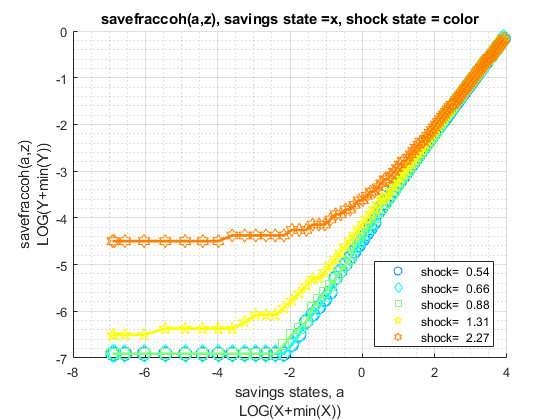
\includegraphics[width=5.20833in,height=\textheight]{img/fx_vfi_az_loop_images/figure_3.png}

When risk aversion increases, at every state-space point, the household
wants to save more.

\begin{verbatim}
% Higher Risk Aversion
mp_params('fl_crra') = 5;
ff_vfi_az_loop(mp_params, mp_support);

Elapsed time is 2.680109 seconds.
----------------------------------------
xxxxxxxxxxxxxxxxxxxxxxxxxxxxxxxxxxxxxxxx
CONTAINER NAME: mp_ffcmd ND Array (Matrix etc)
xxxxxxxxxxxxxxxxxxxxxxxxxxxxxxxxxxxxxxxx
                   i    idx    ndim    numel    rowN    colN     sum       mean        std      coefvari    min      max  
                   _    ___    ____    _____    ____    ____    ______    _______    _______    ________    ___    _______

    savefraccoh    1     1      2       700     100      7      500.59    0.71513    0.25488    0.35641      0     0.94324

xxx TABLE:savefraccoh xxxxxxxxxxxxxxxxxx
              c1         c2          c3         c4         c5         c6         c7   
            _______    _______    ________    _______    _______    _______    _______

    r1            0          0    0.044811    0.15534    0.25694    0.40177    0.48276
    r2            0          0    0.044787    0.15528    0.25686    0.40168    0.48268
    r3            0          0    0.044678    0.15499     0.2565    0.40124    0.48228
    r4            0          0    0.044445    0.15437    0.25572    0.40032    0.48143
    r5            0          0    0.064784    0.15337    0.25445    0.39879    0.48003
    r96     0.92489    0.92134     0.94129    0.93513    0.92717    0.91691    0.92776
    r97     0.92544    0.92198      0.9418     0.9358    0.92802    0.91801    0.92895
    r98     0.92598     0.9226      0.9423    0.93644    0.92885    0.91908     0.9301
    r99      0.9265     0.9232     0.94278    0.93706    0.92965    0.92011    0.93121
    r100      0.927    0.92379     0.94324    0.93765    0.93042     0.9211    0.90914
\end{verbatim}

\includegraphics[width=5.20833in,height=\textheight]{img/fx_vfi_az_loop_images/figure_4.png}

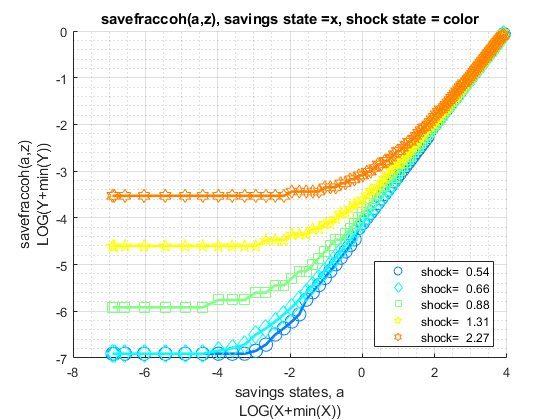
\includegraphics[width=5.20833in,height=\textheight]{img/fx_vfi_az_loop_images/figure_5.png}

\hypertarget{test-ff_vfi_az_loop-with-higher-uncertainty}{%
\subsection{Test FF\_VFI\_AZ\_LOOP with Higher Uncertainty}\label{test-ff_vfi_az_loop-with-higher-uncertainty}}

Increase the standard deviation of the Shock.

\begin{verbatim}
mp_support = containers.Map('KeyType','char', 'ValueType','any');
mp_support('bl_print_params') = false;
mp_support('bl_print_iterinfo') = false;
mp_support('ls_ffcmd') = {'savefraccoh'};
mp_support('ls_ffsna') = {};
mp_support('ls_ffgrh') = {};
mp_params = containers.Map('KeyType','char', 'ValueType','any');
mp_params('it_a_n') = 150;
mp_params('it_z_n') = 15;
mp_params('fl_a_max') = 50;
mp_params('st_grid_type') = 'grid_powerspace';
% graph color spectrum
mp_params('cl_colors') = 'copper';
\end{verbatim}

Lower standard deviation of shock:

\begin{verbatim}
% Lower Risk Aversion
mp_params('fl_shk_std') = 0.10;
ff_vfi_az_loop(mp_params, mp_support);

Elapsed time is 13.492999 seconds.
----------------------------------------
xxxxxxxxxxxxxxxxxxxxxxxxxxxxxxxxxxxxxxxx
CONTAINER NAME: mp_ffcmd ND Array (Matrix etc)
xxxxxxxxxxxxxxxxxxxxxxxxxxxxxxxxxxxxxxxx
                   i    idx    ndim    numel    rowN    colN     sum       mean        std      coefvari    min      max  
                   _    ___    ____    _____    ____    ____    ______    _______    _______    ________    ___    _______

    savefraccoh    1     1      2      2250     150      15     1506.3    0.66947    0.28673     0.4283      0     0.93222

xxx TABLE:savefraccoh xxxxxxxxxxxxxxxxxx
              c1         c2         c3         c4         c5         c11        c12        c13        c14        c15  
            _______    _______    _______    _______    _______    _______    _______    _______    _______    _______

    r1            0          0          0          0          0    0.14061     0.1891    0.24154     0.2699    0.32439
    r2            0          0          0          0          0     0.1406    0.18908    0.24152    0.26988    0.32437
    r3            0          0          0          0          0    0.14053      0.189    0.24142    0.26977    0.32426
    r4            0          0          0          0          0    0.14038    0.18881     0.2412    0.26956    0.32402
    r5            0          0          0          0          0    0.14013    0.18851    0.24085     0.2692    0.32362
    r146    0.93087    0.92957    0.92815    0.92661    0.92492    0.92712    0.92403    0.92069    0.91706    0.91312
    r147    0.93121    0.92994    0.92854    0.92702    0.92537    0.92768    0.92465    0.92135    0.91778    0.91391
    r148    0.93156     0.9303    0.92893    0.92743    0.92581    0.92823    0.92525    0.92201    0.91849    0.91467
    r149    0.93189    0.93065     0.9293    0.92783    0.92623    0.92878    0.92584    0.92264    0.91918    0.91542
    r150    0.93222      0.931    0.92967    0.92823    0.92665     0.9293    0.92641    0.92327    0.91986    0.91616
\end{verbatim}

Higher shock standard deviation: low shock high asset save more, high
shock more asset save less, high shock low asset save more:

\begin{verbatim}
% Higher Risk Aversion
mp_params('fl_shk_std') = 0.40;
ff_vfi_az_loop(mp_params, mp_support);

Elapsed time is 18.680264 seconds.
----------------------------------------
xxxxxxxxxxxxxxxxxxxxxxxxxxxxxxxxxxxxxxxx
CONTAINER NAME: mp_ffcmd ND Array (Matrix etc)
xxxxxxxxxxxxxxxxxxxxxxxxxxxxxxxxxxxxxxxx
                   i    idx    ndim    numel    rowN    colN     sum       mean        std      coefvari    min      max  
                   _    ___    ____    _____    ____    ____    ______    _______    _______    ________    ___    _______

    savefraccoh    1     1      2      2250     150      15     1678.8    0.74614    0.22779    0.30529      0     0.93141

xxx TABLE:savefraccoh xxxxxxxxxxxxxxxxxx
              c1         c2         c3         c4         c5         c11        c12        c13        c14        c15  
            _______    _______    _______    _______    _______    _______    _______    _______    _______    _______

    r1            0          0          0          0          0    0.53612    0.59853    0.67884    0.73891    0.77675
    r2            0          0          0          0          0    0.53609     0.5985    0.67882    0.73889    0.77674
    r3            0          0          0          0          0    0.53594    0.59839    0.67873    0.73883    0.77669
    r4            0          0          0          0          0    0.53563    0.59814    0.67853    0.73868    0.77658
    r5            0          0          0          0          0    0.53511    0.59774    0.67821    0.73843     0.7764
    r146    0.92696     0.9262    0.92513    0.92359    0.92142    0.91653     0.9078    0.88992    0.86057    0.80415
    r147    0.92721    0.92647    0.92541     0.9239    0.92176    0.91741    0.90895    0.89144    0.84828    0.79341
    r148    0.92746    0.92673    0.92569    0.92421     0.9221    0.91827    0.91007    0.87813    0.83621    0.78284
    r149     0.9277    0.92698    0.92596     0.9245    0.92243     0.9191    0.89605    0.86507    0.82436    0.77245
    r150    0.92794    0.92724    0.92623     0.9248    0.92276    0.90467    0.88233    0.85227    0.81273    0.76223
\end{verbatim}

\hypertarget{ff_vfi_az_vec-savings-vectorized-grid-examples}{%
\section{FF\_VFI\_AZ\_VEC Savings Vectorized Grid Examples}\label{ff_vfi_az_vec-savings-vectorized-grid-examples}}

\begin{quote}
Go back to \href{http://fanwangecon.github.io/}{fan}'s \href{https://fanwangecon.github.io/MEconTools/}{MEconTools} Toolbox (\href{https://fanwangecon.github.io/MEconTools/bookdown}{bookdown}), \href{https://fanwangecon.github.io/M4Econ/}{Matlab Code Examples} Repository (\href{https://fanwangecon.github.io/M4Econ/bookdown}{bookdown}), or \href{https://fanwangecon.github.io/Math4Econ/}{Math for Econ with Matlab} Repository (\href{https://fanwangecon.github.io/Math4Econ/bookdown}{bookdown}).
\end{quote}

This is the example vignette for function:
\href{https://github.com/FanWangEcon/MEconTools/blob/master/MEconTools/vfi/ff_vfi_az_vec.m}{\textbf{ff\_vfi\_az\_vec}}
from the \href{https://fanwangecon.github.io/MEconTools/}{\textbf{MEconTools
Package}}\textbf{.} This function
solves the dynamic programming problem for a (a,z) model. Households can
save a, and face AR(1) shock z. The problem is solved over the infinite
horizon.

This is the \textbf{vectorized} code, its speed is much faster than the
looped code. The function is designed to have small memory footprint and
requires low computing resources, yet is fast.

The code uses \textbf{common grid}, with the same state space and choice
space grids.
\href{https://github.com/FanWangEcon/MEconTools/blob/master/MEconTools/vfi/ff_vfi_az_bisec_vec.m}{\textbf{ff\_vfi\_az\_bisec\_vec}}
from the \href{https://fanwangecon.github.io/MEconTools/}{\textbf{MEconTools
Package}} solves the same
problem but using continuous exact percentage asset choices, which is
more precise than the solution here, and perhaps a little bit slower and
relies on First Order Conditions. The
\href{https://github.com/FanWangEcon/MEconTools/blob/master/MEconTools/vfi/ff_vfi_az_mzoom_vec.m}{\textbf{ff\_vfi\_az\_mzoom\_vec}}
also solves the same class of problems with continuous exact percentage
asset choices, and does not rely on First Order Conditions, but is
slower than
\href{https://github.com/FanWangEcon/MEconTools/blob/master/MEconTools/vfi/ff_vfi_az_bisec_vec.m}{\textbf{ff\_vfi\_az\_bisec\_vec}}\textbf{.}

\textbf{Links to Other Code:}

Core Savings/Borrowing Dynamic Programming Solution Functions that are
functions in the \href{https://fanwangecon.github.io/MEconTools/}{\textbf{MEconTools
Package}}\textbf{.} :

\begin{itemize}
\item
  Common Choice and States Grid :
  \href{https://github.com/FanWangEcon/MEconTools/blob/master/MEconTools/vfi/ff_vfi_az_loop.m}{\textbf{ff\_vfi\_az\_loop}}
\item
  Common Choice and States Grid :
  \href{https://github.com/FanWangEcon/MEconTools/blob/master/MEconTools/vfi/ff_vfi_az_vec.m}{\textbf{ff\_vfi\_az\_vec}}
\item
  States Grid + Continuous Exact Savings as Share of Cash-on-Hand,
  rely on FOC, :\href{https://github.com/FanWangEcon/MEconTools/blob/master/MEconTools/vfi/ff_vfi_az_bisec_loop.m}{\textbf{ff\_vfi\_az\_bisec\_loop}}
\item
  States Grid + Continuous Exact Savings as Share of Cash-on-Hand,
  rely on FOC :
  \href{https://github.com/FanWangEcon/MEconTools/blob/master/MEconTools/vfi/ff_vfi_az_bisec_vec.m}{\textbf{ff\_vfi\_az\_bisec\_vec}}
\item
  States Grid + Continuous Exact Savings as Share of Cash-on-Hand,
  VALUE comparison, :\href{https://github.com/FanWangEcon/MEconTools/blob/master/MEconTools/vfi/ff_vfi_az_mzoom_loop.m}{\textbf{ff\_vfi\_az\_mzoom\_loop}}
\item
  States Grid + Continuous Exact Savings as Share of Cash-on-Hand,
  VALUE comparison, :
  \href{https://github.com/FanWangEcon/MEconTools/blob/master/MEconTools/vfi/ff_vfi_az_mzoom_vec.m}{\textbf{ff\_vfi\_az\_mzoom\_vec}}
\end{itemize}

\hypertarget{test-ff_vfi_az_vec-defaults}{%
\subsection{Test FF\_VFI\_AZ\_VEC Defaults}\label{test-ff_vfi_az_vec-defaults}}

Call the function with defaults. By default, shows the asset policy
function summary. Model parameters can be changed by the mp\_params.

\begin{verbatim}
%mp_params
mp_params = containers.Map('KeyType','char', 'ValueType','any');
mp_params('fl_crra') = 1.5;
mp_params('fl_beta') = 0.94;
ff_vfi_az_vec(mp_params);

Elapsed time is 0.136223 seconds.
----------------------------------------
xxxxxxxxxxxxxxxxxxxxxxxxxxxxxxxxxxxxxxxx
CONTAINER NAME: mp_ffcmd ND Array (Matrix etc)
xxxxxxxxxxxxxxxxxxxxxxxxxxxxxxxxxxxxxxxx
          i    idx    ndim    numel    rowN    colN     sum       mean      std      coefvari    min    max
          _    ___    ____    _____    ____    ____    ______    ______    ______    ________    ___    ___

    ap    1     1      2       700     100      7      9855.1    14.079    14.408     1.0234      0     50 

xxx TABLE:ap xxxxxxxxxxxxxxxxxx
              c1        c2        c3         c4         c5         c6         c7  
            ______    ______    ______    ________    _______    _______    ______

    r1           0         0         0    0.045213    0.25576    0.61095    1.0362
    r2           0         0         0    0.045213    0.25576    0.61095    1.0362
    r3           0         0         0    0.045213    0.25576    0.61095    1.0362
    r4           0         0         0     0.06647    0.25576    0.61095    1.0362
    r5           0         0         0     0.06647    0.25576    0.61095     1.164
    r96     43.924    43.924    43.924      43.924     43.924     45.102    45.102
    r97     45.102    45.102    45.102      45.102     45.102     46.298    46.298
    r98     46.298    46.298    46.298      46.298     46.298     47.513    47.513
    r99     47.513    47.513    47.513      47.513     47.513     48.747    48.747
    r100    48.747    48.747    48.747      48.747     48.747         50        50
\end{verbatim}

\hypertarget{test-ff_vfi_az_bisec_vec-speed-tests-1}{%
\subsection{Test FF\_VFI\_AZ\_BISEC\_VEC Speed Tests}\label{test-ff_vfi_az_bisec_vec-speed-tests-1}}

Call the function with different a and z grid size, print out speed:

\begin{verbatim}
mp_support = containers.Map('KeyType','char', 'ValueType','any');
mp_support('bl_timer') = true;
mp_support('ls_ffcmd') = {};
% A grid 50, shock grid 5:
mp_params = containers.Map('KeyType','char', 'ValueType','any');
mp_params('it_a_n') = 50;
mp_params('it_z_n') = 5;
ff_vfi_az_vec(mp_params, mp_support);

Elapsed time is 0.025309 seconds.

% A grid 750, shock grid 15:
mp_params = containers.Map('KeyType','char', 'ValueType','any');
mp_params('it_a_n') = 750;
mp_params('it_z_n') = 15;
ff_vfi_az_vec(mp_params, mp_support);

Elapsed time is 4.855482 seconds.

% A grid 600, shock grid 45:
mp_params = containers.Map('KeyType','char', 'ValueType','any');
mp_params('it_a_n') = 600;
mp_params('it_z_n') = 45;
ff_vfi_az_vec(mp_params, mp_support);

Elapsed time is 12.201130 seconds.
\end{verbatim}

\hypertarget{test-ff_vfi_az_vec-control-outputs}{%
\subsection{Test FF\_VFI\_AZ\_VEC Control Outputs}\label{test-ff_vfi_az_vec-control-outputs}}

Run the function first without any outputs, but only the timer.

\begin{verbatim}
mp_params = containers.Map('KeyType','char', 'ValueType','any');
mp_params('it_a_n') = 50;
mp_params('it_z_n') = 5;
mp_support = containers.Map('KeyType','char', 'ValueType','any');
mp_support('bl_timer') = true;
mp_support('bl_print_params') = false;
mp_support('bl_print_iterinfo') = false;
mp_support('ls_ffcmd') = {};
ff_vfi_az_vec(mp_params, mp_support);

Elapsed time is 0.022504 seconds.
\end{verbatim}

Run the function and show policy function for savings choice. For
ls\_ffcmd, ls\_ffsna, ls\_ffgrh, can include these: `v', `ap', `c', `y',
`coh', `savefraccoh'. These are value, aprime savings choice,
consumption, income, cash on hand, and savings fraction as cash-on-hand.

\begin{verbatim}
mp_support = containers.Map('KeyType','char', 'ValueType','any');
mp_support('bl_print_params') = false;
mp_support('bl_print_iterinfo') = false;
% ls_ffcmd: summary print which outcomes
mp_support('ls_ffcmd') = {};
% ls_ffsna: detail print which outcomes
mp_support('ls_ffsna') = {'savefraccoh'};
% ls_ffgrh: graphical print which outcomes
mp_support('ls_ffgrh') = {'savefraccoh'};
ff_vfi_az_vec(mp_params, mp_support);

Elapsed time is 0.041571 seconds.
xxx  ff_vfi_az_vec, outcome=savefraccoh  xxxxxxxxxxxxxxxxxxxxxxxxxxx
    group       a        mean_z_0_4858    mean_z_0_67798    mean_z_0_9462    mean_z_1_3205    mean_z_1_8429
    _____    ________    _____________    ______________    _____________    _____________    _____________

      1             0              0                0         0.071865          0.20862          0.36462   
      2      0.002975              0                0         0.071698          0.20827          0.36418   
      3      0.016829              0                0         0.070928          0.20666          0.36216   
      4      0.046375              0        0.0029827         0.069341          0.20331          0.35793   
      5      0.095198      0.0038183         0.044243          0.11681          0.27649          0.35114   
      6        0.1663       0.054362         0.084837          0.17517          0.26637          0.34171   
      7       0.26234       0.099899          0.13609          0.16422          0.25383          0.41847   
      8       0.38568        0.15381          0.19428          0.22348          0.32132          0.40047   
      9       0.53852        0.21153          0.25554          0.28573          0.39055          0.47258   
     10       0.72291        0.26934          0.31659          0.34814          0.36175          0.44538   
     11       0.94076         0.3247          0.37504          0.40848          0.42229          0.50941   
     12        1.1939        0.37617          0.42941          0.46521           0.4802          0.57087   
     13         1.484        0.53695          0.47898          0.51743           0.5344           0.5291   
     14        1.8128        0.57847          0.52356          0.56473          0.58429          0.58056   
     15        2.1817        0.61468          0.56329           0.6071          0.62958          0.62823   
     16        2.5924         0.6462           0.5985          0.64475          0.67028          0.67186   
     17        3.0463        0.67365          0.62963          0.67804          0.60721          0.71141   
     18        3.5449        0.69762          0.65713          0.70737           0.6404          0.65255   
     19        4.0894        0.71859          0.68142          0.73318          0.67021          0.68509   
     20        4.6813        0.73701          0.70293          0.75587           0.6969          0.71446   
     21        5.3218        0.75325            0.722          0.77584          0.72078          0.74089   
     22        6.0121        0.76763          0.73895          0.79344          0.74211          0.76461   
     23        6.7536         0.7804          0.75407          0.80897          0.76119          0.78587   
     24        7.5474         0.7918          0.76759           0.8227          0.77824          0.80491   
     25        8.3948        0.80201          0.77972          0.83486          0.79351          0.82194   
     26        9.2967        0.81119          0.79063          0.84567          0.80719          0.83719   
     27        10.254        0.81947          0.80049           0.8553          0.81948          0.85083   
     28        11.269        0.82697          0.80941          0.86389          0.83053          0.86306   
     29        12.342        0.83379          0.81752          0.87159          0.84048          0.87401   
     30        13.473        0.84001           0.8249          0.87849          0.84946          0.88384   
     31        14.665        0.84569          0.83165           0.8847          0.85759          0.82241   
     32        15.918         0.8509          0.83782           0.8903          0.86495          0.83188   
     33        17.233         0.8557           0.8435          0.89536          0.87163          0.84053   
     34        18.611        0.86012          0.84872          0.89995           0.8777          0.84844   
     35        20.053        0.86421          0.85354          0.90411          0.88324          0.85568   
     36         21.56        0.86799            0.858           0.9079           0.8883          0.86231   
     37        23.133        0.87151          0.86214          0.91136          0.89292          0.86841   
     38        24.773        0.87479          0.86598          0.91452          0.89716          0.87401   
     39        26.481        0.87784          0.86955          0.91741          0.90105          0.87917   
     40        28.258         0.8807          0.87289          0.92007          0.90463          0.88393   
     41        30.104        0.88337          0.87601          0.92251          0.90793          0.88833   
     42        32.021        0.88588          0.87893          0.92475          0.91097           0.8924   
     43         34.01        0.88824          0.88166          0.92683          0.91378          0.89617   
     44         36.07        0.89046          0.88423          0.92874          0.91638          0.89966   
     45        38.204        0.89256          0.88665          0.93052          0.91879          0.90291   
     46        40.412        0.89453           0.9403          0.93216          0.92102          0.90592   
     47        42.695         0.8964          0.94141          0.93368           0.9231          0.90873   
     48        45.053        0.89817          0.94245           0.9351          0.92504          0.91135   
     49        47.488        0.89985          0.94341          0.93642          0.92684           0.9138   
     50            50        0.90144           0.9443          0.93765          0.92853          0.91608   
\end{verbatim}

\includegraphics[width=5.20833in,height=\textheight]{img/fx_vfi_az_vec_images/figure_0.png}

\includegraphics[width=5.20833in,height=\textheight]{img/fx_vfi_az_vec_images/figure_1.png}

Run the function and show summaries for savings and fraction of coh
saved:

\begin{verbatim}
mp_params('it_a_n') = 100;
mp_params('it_z_n') = 9;
mp_support('ls_ffcmd') = {'ap', 'savefraccoh'};
mp_support('ls_ffsna') = {};
mp_support('ls_ffgrh') = {};
mp_support('bl_vfi_store_all') = true; % store c(a,z), y(a,z)
ff_vfi_az_vec(mp_params, mp_support);

Elapsed time is 0.230510 seconds.
----------------------------------------
xxxxxxxxxxxxxxxxxxxxxxxxxxxxxxxxxxxxxxxx
CONTAINER NAME: mp_ffcmd ND Array (Matrix etc)
xxxxxxxxxxxxxxxxxxxxxxxxxxxxxxxxxxxxxxxx
                   i    idx    ndim    numel    rowN    colN     sum       mean        std      coefvari    min      max  
                   _    ___    ____    _____    ____    ____    ______    _______    _______    ________    ___    _______

    ap             1     1      2       900     100      9       12904     14.338     14.524      1.013      0          50
    savefraccoh    2     2      2       900     100      9      619.51    0.68834    0.26953    0.39157      0     0.93151

xxx TABLE:ap xxxxxxxxxxxxxxxxxx
              c1        c2        c3          c4           c5         c6         c7         c8        c9  
            ______    ______    ______    __________    ________    _______    _______    ______    ______

    r1           0         0         0             0    0.092813    0.25576    0.61095    1.0362    1.6023
    r2           0         0         0             0    0.092813    0.25576    0.61095    1.0362    1.6023
    r3           0         0         0             0    0.092813    0.25576    0.61095    1.0362    1.6023
    r4           0         0         0    0.00051272    0.092813    0.25576    0.61095    1.0362    1.6023
    r5           0         0         0     0.0029004    0.092813    0.25576    0.61095    1.0362    1.6023
    r96     43.924    43.924    43.924        43.924      43.924     45.102     45.102    45.102    46.298
    r97     45.102    45.102    45.102        45.102      45.102     46.298     46.298    46.298    47.513
    r98     46.298    46.298    46.298        46.298      46.298     47.513     47.513    47.513    48.747
    r99     47.513    47.513    47.513        47.513      47.513     48.747     48.747    48.747        50
    r100    48.747    48.747    48.747        48.747      48.747         50         50        50        50

xxx TABLE:savefraccoh xxxxxxxxxxxxxxxxxx
              c1         c2         c3           c4           c5         c6         c7         c8         c9   
            _______    _______    _______    __________    ________    _______    _______    _______    _______

    r1            0          0          0             0    0.070073    0.15255    0.28789    0.38573    0.47121
    r2            0          0          0             0    0.070045     0.1525    0.28781    0.38565    0.47114
    r3            0          0          0             0    0.069914    0.15228    0.28748     0.3853     0.4708
    r4            0          0          0    0.00048613    0.069636     0.1518    0.28676    0.38454    0.47007
    r5            0          0          0     0.0027273    0.069182    0.15101    0.28559    0.38329    0.46886
    r96     0.92625    0.92358    0.92022         0.916     0.91072    0.92836    0.91992    0.90945    0.92033
    r97     0.92676    0.92416    0.92088       0.91677     0.91162    0.92918    0.92095    0.91073    0.92169
    r98     0.92727    0.92473    0.92153       0.91752     0.91249    0.92998    0.92194    0.91196      0.923
    r99     0.92776    0.92528    0.92216       0.91824     0.91333    0.93076    0.92291    0.91315    0.92426
    r100    0.92823    0.92581    0.92277       0.91895     0.91416    0.93151    0.92384    0.91431    0.90252
\end{verbatim}

\hypertarget{test-ff_vfi_az_vec-change-interest-rate-and-discount}{%
\subsection{Test FF\_VFI\_AZ\_VEC Change Interest Rate and Discount}\label{test-ff_vfi_az_vec-change-interest-rate-and-discount}}

Show only save fraction of cash on hand:

\begin{verbatim}
mp_support = containers.Map('KeyType','char', 'ValueType','any');
mp_support('bl_print_params') = false;
mp_support('bl_print_iterinfo') = false;
mp_support('ls_ffcmd') = {'savefraccoh'};
mp_support('ls_ffsna') = {};
mp_support('ls_ffgrh') = {};
mp_params = containers.Map('KeyType','char', 'ValueType','any');
mp_params('it_a_n') = 100;
mp_params('it_z_n') = 7;
mp_params('fl_a_max') = 50;
mp_params('st_grid_type') = 'grid_powerspace';
\end{verbatim}

Solve the model with several different interest rates and discount
factor:

\begin{verbatim}
% Lower Savings Incentives
mp_params('fl_beta') = 0.80;
mp_params('fl_r') = 0.01;
ff_vfi_az_vec(mp_params, mp_support);

Elapsed time is 0.058079 seconds.
----------------------------------------
xxxxxxxxxxxxxxxxxxxxxxxxxxxxxxxxxxxxxxxx
CONTAINER NAME: mp_ffcmd ND Array (Matrix etc)
xxxxxxxxxxxxxxxxxxxxxxxxxxxxxxxxxxxxxxxx
                   i    idx    ndim    numel    rowN    colN     sum       mean      std      coefvari    min      max  
                   _    ___    ____    _____    ____    ____    ______    ______    ______    ________    ___    _______

    savefraccoh    1     1      2       700     100      7      357.49    0.5107    0.2755    0.53945      0     0.80531

xxx TABLE:savefraccoh xxxxxxxxxxxxxxxxxx
              c1         c2         c3         c4         c5           c6           c7   
            _______    _______    _______    _______    _______    __________    ________

    r1            0          0          0          0          0     0.0002246    0.041573
    r2            0          0          0          0          0    0.00022455    0.041566
    r3            0          0          0          0          0     0.0012689    0.041533
    r4            0          0          0          0          0      0.001266    0.041462
    r5            0          0          0          0          0     0.0034759    0.041345
    r96     0.78455    0.78145    0.79995    0.79456     0.7876       0.77865     0.76719
    r97     0.78669    0.78366    0.77972    0.79679    0.78998       0.78122     0.77001
    r98     0.78878    0.78582    0.78197    0.79897    0.79231       0.78374     0.77276
    r99     0.79084    0.78794    0.78417    0.77927    0.79459        0.7862     0.77545
    r100    0.79285    0.79001    0.78633    0.78154    0.79682        0.7886     0.77808

% Higher Savings Incentives
mp_params('fl_beta') = 0.95;
mp_params('fl_r') = 0.04;
ff_vfi_az_vec(mp_params, mp_support);

Elapsed time is 0.177867 seconds.
----------------------------------------
xxxxxxxxxxxxxxxxxxxxxxxxxxxxxxxxxxxxxxxx
CONTAINER NAME: mp_ffcmd ND Array (Matrix etc)
xxxxxxxxxxxxxxxxxxxxxxxxxxxxxxxxxxxxxxxx
                   i    idx    ndim    numel    rowN    colN     sum       mean        std      coefvari    min      max  
                   _    ___    ____    _____    ____    ____    ______    _______    _______    ________    ___    _______

    savefraccoh    1     1      2       700     100      7      479.94    0.68563    0.27152    0.39602      0     0.93121

xxx TABLE:savefraccoh xxxxxxxxxxxxxxxxxx
              c1         c2           c3           c4         c5         c6         c7   
            _______    _______    __________    ________    _______    _______    _______

    r1            0          0             0     0.07007    0.17967    0.30874    0.43404
    r2            0          0             0    0.070042    0.17961    0.30866    0.43396
    r3            0          0             0    0.069911    0.17935    0.30833     0.4336
    r4            0          0             0    0.069633    0.17881    0.30762    0.43284
    r5            0          0    0.00049972    0.069179    0.17792    0.30645    0.43158
    r96     0.92489    0.92134       0.91672     0.91072    0.92717    0.91691    0.92776
    r97     0.92544    0.92198       0.91747     0.91162    0.92802    0.91801    0.92895
    r98     0.92598     0.9226        0.9182     0.91249    0.92885    0.91908     0.9301
    r99      0.9265     0.9232       0.91891     0.91333    0.92965    0.92011    0.93121
    r100      0.927    0.92379        0.9196     0.91416    0.93042     0.9211    0.90914
\end{verbatim}

\hypertarget{test-ff_vfi_az_vec-changing-risk-aversion}{%
\subsection{Test FF\_VFI\_AZ\_VEC Changing Risk Aversion}\label{test-ff_vfi_az_vec-changing-risk-aversion}}

Here, again, show fraction of coh saved in summary tabular form, but
also show it graphically.

\begin{verbatim}
mp_support = containers.Map('KeyType','char', 'ValueType','any');
mp_support('bl_print_params') = false;
mp_support('bl_print_iterinfo') = false;
mp_support('ls_ffcmd') = {'savefraccoh'};
mp_support('ls_ffsna') = {};
mp_support('ls_ffgrh') = {'savefraccoh'};
mp_params = containers.Map('KeyType','char', 'ValueType','any');
mp_params('it_a_n') = 100;
mp_params('it_z_n') = 7;
mp_params('fl_a_max') = 50;
mp_params('st_grid_type') = 'grid_powerspace';
\end{verbatim}

Solve the model with different risk aversion levels, higher preferences
for risk:

\begin{verbatim}
% Lower Risk Aversion
mp_params('fl_crra') = 0.5;
ff_vfi_az_vec(mp_params, mp_support);

Elapsed time is 0.181638 seconds.
----------------------------------------
xxxxxxxxxxxxxxxxxxxxxxxxxxxxxxxxxxxxxxxx
CONTAINER NAME: mp_ffcmd ND Array (Matrix etc)
xxxxxxxxxxxxxxxxxxxxxxxxxxxxxxxxxxxxxxxx
                   i    idx    ndim    numel    rowN    colN     sum       mean       std      coefvari    min      max  
                   _    ___    ____    _____    ____    ____    ______    _______    ______    ________    ___    _______

    savefraccoh    1     1      2       700     100      7      450.35    0.64336    0.2803    0.43568      0     0.90711

xxx TABLE:savefraccoh xxxxxxxxxxxxxxxxxx
              c1         c2         c3          c4           c5         c6         c7   
            _______    _______    _______    _________    ________    _______    _______

    r1            0          0          0    0.0060341    0.093241    0.19572    0.30604
    r2            0          0          0    0.0060316    0.093213    0.19567    0.30599
    r3            0          0          0    0.0060204     0.09308    0.19546    0.30574
    r4            0          0          0    0.0059964    0.092798    0.19501     0.3052
    r5            0          0          0     0.012229    0.092335    0.19427    0.30431
    r96     0.90049    0.89703    0.89253      0.88669     0.90296    0.89297    0.90379
    r97     0.90128    0.89791    0.89351      0.88781     0.90404    0.89429    0.88181
    r98     0.90205    0.89876    0.89447      0.88891      0.9051    0.89557    0.88337
    r99      0.9028    0.89959    0.89541      0.88998     0.90612    0.89681    0.88489
    r100    0.90354     0.9004    0.89632      0.89101     0.90711    0.89802    0.88636
\end{verbatim}

\includegraphics[width=5.20833in,height=\textheight]{img/fx_vfi_az_vec_images/figure_2.png}

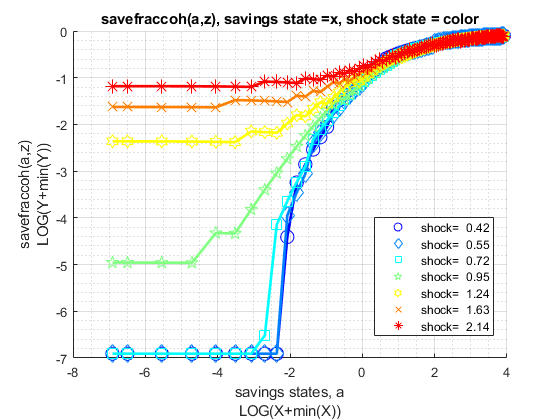
\includegraphics[width=5.20833in,height=\textheight]{img/fx_vfi_az_vec_images/figure_3.png}

When risk aversion increases, at every state-space point, the household
wants to save more.

\begin{verbatim}
% Higher Risk Aversion
mp_params('fl_crra') = 5;
ff_vfi_az_vec(mp_params, mp_support);

Elapsed time is 0.152901 seconds.
----------------------------------------
xxxxxxxxxxxxxxxxxxxxxxxxxxxxxxxxxxxxxxxx
CONTAINER NAME: mp_ffcmd ND Array (Matrix etc)
xxxxxxxxxxxxxxxxxxxxxxxxxxxxxxxxxxxxxxxx
                   i    idx    ndim    numel    rowN    colN     sum       mean        std      coefvari    min      max  
                   _    ___    ____    _____    ____    ____    ______    _______    _______    ________    ___    _______

    savefraccoh    1     1      2       700     100      7      500.59    0.71513    0.25488    0.35641      0     0.94324

xxx TABLE:savefraccoh xxxxxxxxxxxxxxxxxx
              c1         c2          c3         c4         c5         c6         c7   
            _______    _______    ________    _______    _______    _______    _______

    r1            0          0    0.044811    0.15534    0.25694    0.40177    0.48276
    r2            0          0    0.044787    0.15528    0.25686    0.40168    0.48268
    r3            0          0    0.044678    0.15499     0.2565    0.40124    0.48228
    r4            0          0    0.044445    0.15437    0.25572    0.40032    0.48143
    r5            0          0    0.064784    0.15337    0.25445    0.39879    0.48003
    r96     0.92489    0.92134     0.94129    0.93513    0.92717    0.91691    0.92776
    r97     0.92544    0.92198      0.9418     0.9358    0.92802    0.91801    0.92895
    r98     0.92598     0.9226      0.9423    0.93644    0.92885    0.91908     0.9301
    r99      0.9265     0.9232     0.94278    0.93706    0.92965    0.92011    0.93121
    r100      0.927    0.92379     0.94324    0.93765    0.93042     0.9211    0.90914
\end{verbatim}

\includegraphics[width=5.20833in,height=\textheight]{img/fx_vfi_az_vec_images/figure_4.png}

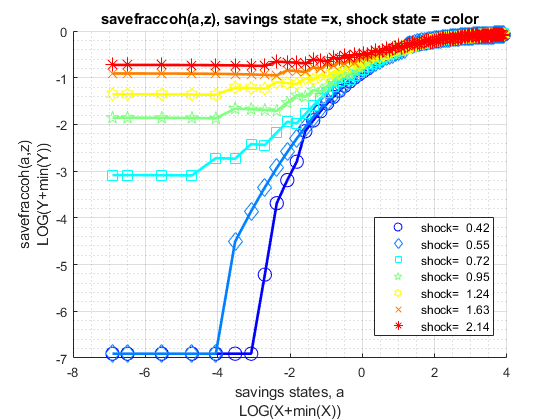
\includegraphics[width=5.20833in,height=\textheight]{img/fx_vfi_az_vec_images/figure_5.png}

\hypertarget{test-ff_vfi_az_vec-with-higher-uncertainty}{%
\subsection{Test FF\_VFI\_AZ\_VEC with Higher Uncertainty}\label{test-ff_vfi_az_vec-with-higher-uncertainty}}

Increase the standard deviation of the Shock.

\begin{verbatim}
mp_support = containers.Map('KeyType','char', 'ValueType','any');
mp_support('bl_print_params') = false;
mp_support('bl_print_iterinfo') = false;
mp_support('ls_ffcmd') = {'savefraccoh'};
mp_support('ls_ffsna') = {};
mp_support('ls_ffgrh') = {};
mp_params = containers.Map('KeyType','char', 'ValueType','any');
mp_params('it_a_n') = 150;
mp_params('it_z_n') = 15;
mp_params('fl_a_max') = 50;
mp_params('st_grid_type') = 'grid_powerspace';
% graph color spectrum
mp_params('cl_colors') = 'copper';
\end{verbatim}

Lower standard deviation of shock:

\begin{verbatim}
% Lower Risk Aversion
mp_params('fl_shk_std') = 0.10;
ff_vfi_az_vec(mp_params, mp_support);

Elapsed time is 0.544499 seconds.
----------------------------------------
xxxxxxxxxxxxxxxxxxxxxxxxxxxxxxxxxxxxxxxx
CONTAINER NAME: mp_ffcmd ND Array (Matrix etc)
xxxxxxxxxxxxxxxxxxxxxxxxxxxxxxxxxxxxxxxx
                   i    idx    ndim    numel    rowN    colN     sum       mean        std      coefvari    min      max  
                   _    ___    ____    _____    ____    ____    ______    _______    _______    ________    ___    _______

    savefraccoh    1     1      2      2250     150      15     1506.3    0.66947    0.28673     0.4283      0     0.93222

xxx TABLE:savefraccoh xxxxxxxxxxxxxxxxxx
              c1         c2         c3         c4         c5         c11        c12        c13        c14        c15  
            _______    _______    _______    _______    _______    _______    _______    _______    _______    _______

    r1            0          0          0          0          0    0.14061     0.1891    0.24154     0.2699    0.32439
    r2            0          0          0          0          0     0.1406    0.18908    0.24152    0.26988    0.32437
    r3            0          0          0          0          0    0.14053      0.189    0.24142    0.26977    0.32426
    r4            0          0          0          0          0    0.14038    0.18881     0.2412    0.26956    0.32402
    r5            0          0          0          0          0    0.14013    0.18851    0.24085     0.2692    0.32362
    r146    0.93087    0.92957    0.92815    0.92661    0.92492    0.92712    0.92403    0.92069    0.91706    0.91312
    r147    0.93121    0.92994    0.92854    0.92702    0.92537    0.92768    0.92465    0.92135    0.91778    0.91391
    r148    0.93156     0.9303    0.92893    0.92743    0.92581    0.92823    0.92525    0.92201    0.91849    0.91467
    r149    0.93189    0.93065     0.9293    0.92783    0.92623    0.92878    0.92584    0.92264    0.91918    0.91542
    r150    0.93222      0.931    0.92967    0.92823    0.92665     0.9293    0.92641    0.92327    0.91986    0.91616
\end{verbatim}

Higher shock standard deviation: low shock high asset save more, high
shock more asset save less, high shock low asset save more:

\begin{verbatim}
% Higher Risk Aversion
mp_params('fl_shk_std') = 0.40;
ff_vfi_az_vec(mp_params, mp_support);

Elapsed time is 0.515060 seconds.
----------------------------------------
xxxxxxxxxxxxxxxxxxxxxxxxxxxxxxxxxxxxxxxx
CONTAINER NAME: mp_ffcmd ND Array (Matrix etc)
xxxxxxxxxxxxxxxxxxxxxxxxxxxxxxxxxxxxxxxx
                   i    idx    ndim    numel    rowN    colN     sum       mean        std      coefvari    min      max  
                   _    ___    ____    _____    ____    ____    ______    _______    _______    ________    ___    _______

    savefraccoh    1     1      2      2250     150      15     1678.8    0.74614    0.22779    0.30529      0     0.93141

xxx TABLE:savefraccoh xxxxxxxxxxxxxxxxxx
              c1         c2         c3         c4         c5         c11        c12        c13        c14        c15  
            _______    _______    _______    _______    _______    _______    _______    _______    _______    _______

    r1            0          0          0          0          0    0.53612    0.59853    0.67884    0.73891    0.77675
    r2            0          0          0          0          0    0.53609     0.5985    0.67882    0.73889    0.77674
    r3            0          0          0          0          0    0.53594    0.59839    0.67873    0.73883    0.77669
    r4            0          0          0          0          0    0.53563    0.59814    0.67853    0.73868    0.77658
    r5            0          0          0          0          0    0.53511    0.59774    0.67821    0.73843     0.7764
    r146    0.92696     0.9262    0.92513    0.92359    0.92142    0.91653     0.9078    0.88992    0.86057    0.80415
    r147    0.92721    0.92647    0.92541     0.9239    0.92176    0.91741    0.90895    0.89144    0.84828    0.79341
    r148    0.92746    0.92673    0.92569    0.92421     0.9221    0.91827    0.91007    0.87813    0.83621    0.78284
    r149     0.9277    0.92698    0.92596     0.9245    0.92243     0.9191    0.89605    0.86507    0.82436    0.77245
    r150    0.92794    0.92724    0.92623     0.9248    0.92276    0.90467    0.88233    0.85227    0.81273    0.76223
\end{verbatim}

\hypertarget{ff_vfi_az_bisec_loop-savings-loop-exact-foc-examples}{%
\section{FF\_VFI\_AZ\_BISEC\_LOOP Savings Loop Exact (FOC) Examples}\label{ff_vfi_az_bisec_loop-savings-loop-exact-foc-examples}}

\begin{quote}
Go back to \href{http://fanwangecon.github.io/}{fan}'s \href{https://fanwangecon.github.io/MEconTools/}{MEconTools} Toolbox (\href{https://fanwangecon.github.io/MEconTools/bookdown}{bookdown}), \href{https://fanwangecon.github.io/M4Econ/}{Matlab Code Examples} Repository (\href{https://fanwangecon.github.io/M4Econ/bookdown}{bookdown}), or \href{https://fanwangecon.github.io/Math4Econ/}{Math for Econ with Matlab} Repository (\href{https://fanwangecon.github.io/Math4Econ/bookdown}{bookdown}).
\end{quote}

This is the example vignette for function:\href{https://github.com/FanWangEcon/MEconTools/blob/master/MEconTools/vfi/ff_vfi_az_bisec_loop.m}{\textbf{ff\_vfi\_az\_bisec\_loop}}from
the \href{https://fanwangecon.github.io/MEconTools/}{\textbf{MEconTools
Package}}\textbf{.} This function
solves the dynamic programming problem for a (a,z) model. Households can
save a, and face AR(1) shock z. The problem is solved over the infinite
horizon.

This is the \textbf{looped} code, it is slow for larger state-space problems.

The code uses \textbf{continuous} choices, solved with bisection. The
state-space is on a grid, but choice grids are in terms of \textbf{percentage
of resources} to save and solved exactly.

\textbf{Links to Other Code:}

Core Savings/Borrowing Dynamic Programming Solution Functions that are
functions in the \href{https://fanwangecon.github.io/MEconTools/}{\textbf{MEconTools
Package}}\textbf{.} :

\begin{itemize}
\item
  Common Choice and States Grid :
  \href{https://github.com/FanWangEcon/MEconTools/blob/master/MEconTools/vfi/ff_vfi_az_loop.m}{\textbf{ff\_vfi\_az\_loop}}
\item
  Common Choice and States Grid :
  \href{https://github.com/FanWangEcon/MEconTools/blob/master/MEconTools/vfi/ff_vfi_az_vec.m}{\textbf{ff\_vfi\_az\_vec}}
\item
  States Grid + Continuous Exact Savings as Share of Cash-on-Hand,
  rely on FOC, :\href{https://github.com/FanWangEcon/MEconTools/blob/master/MEconTools/vfi/ff_vfi_az_bisec_loop.m}{\textbf{ff\_vfi\_az\_bisec\_loop}}
\item
  States Grid + Continuous Exact Savings as Share of Cash-on-Hand,
  rely on FOC :
  \href{https://github.com/FanWangEcon/MEconTools/blob/master/MEconTools/vfi/ff_vfi_az_bisec_vec.m}{\textbf{ff\_vfi\_az\_bisec\_vec}}
\item
  States Grid + Continuous Exact Savings as Share of Cash-on-Hand,
  VALUE comparison, :\href{https://github.com/FanWangEcon/MEconTools/blob/master/MEconTools/vfi/ff_vfi_az_mzoom_loop.m}{\textbf{ff\_vfi\_az\_mzoom\_loop}}
\item
  States Grid + Continuous Exact Savings as Share of Cash-on-Hand,
  VALUE comparison, :
  \href{https://github.com/FanWangEcon/MEconTools/blob/master/MEconTools/vfi/ff_vfi_az_mzoom_vec.m}{\textbf{ff\_vfi\_az\_mzoom\_vec}}
\end{itemize}

\hypertarget{test-ff_vfi_az_bisec_loop-defaults}{%
\subsection{Test FF\_VFI\_AZ\_BISEC\_LOOP Defaults}\label{test-ff_vfi_az_bisec_loop-defaults}}

Call the function with defaults. By default, shows the asset policy
function summary. Model parameters can be changed by the mp\_params.

\begin{verbatim}
%mp_params
mp_params = containers.Map('KeyType','char', 'ValueType','any');
mp_params('fl_crra') = 1.5;
mp_params('fl_beta') = 0.94;
% call function
ff_vfi_az_bisec_loop(mp_params);

Elapsed time is 33.158577 seconds.
----------------------------------------
xxxxxxxxxxxxxxxxxxxxxxxxxxxxxxxxxxxxxxxx
CONTAINER NAME: mp_ffcmd ND Array (Matrix etc)
xxxxxxxxxxxxxxxxxxxxxxxxxxxxxxxxxxxxxxxx
          i    idx    ndim    numel    rowN    colN     sum       mean      std      coefvari    min     max  
          _    ___    ____    _____    ____    ____    ______    ______    ______    ________    ___    ______

    ap    1     1      2       700     100      7      9863.4    14.091    14.388     1.0211      0     50.117

xxx TABLE:ap xxxxxxxxxxxxxxxxxx
              c1        c2        c3         c4         c5         c6         c7  
            ______    ______    ______    ________    _______    _______    ______

    r1           0         0         0    0.053491    0.25574    0.60604    1.1157
    r2           0         0         0    0.053998    0.25571     0.6066    1.1163
    r3           0         0         0    0.056449    0.25576    0.60907    1.1187
    r4           0         0         0    0.061799    0.26016     0.6109    1.1239
    r5           0         0         0    0.066463    0.26897    0.61141    1.1327
    r96     43.388     43.52    43.701      43.925     44.222      44.68    45.228
    r97     44.566    44.695    44.878      45.103     45.398     45.856    46.403
    r98     45.761    45.892    46.072      46.298     46.592      47.05    47.597
    r99     46.973    47.107    47.286      47.514     47.806     48.263    48.815
    r100    48.206    48.338    48.519      48.746     49.037     49.497    50.117
\end{verbatim}

\hypertarget{test-ff_vfi_az_bisec_loop-speed-tests}{%
\subsection{Test FF\_VFI\_AZ\_BISEC\_LOOP Speed Tests}\label{test-ff_vfi_az_bisec_loop-speed-tests}}

Call the function with defaults. By default, shows the asset policy
function summary. Model parameters can be changed by the mp\_params.

\begin{verbatim}
mp_support = containers.Map('KeyType','char', 'ValueType','any');
mp_support('bl_timer') = true;
mp_support('ls_ffcmd') = {};
% A grid 50, shock grid 5:
mp_params = containers.Map('KeyType','char', 'ValueType','any');
mp_params('it_a_n') = 50;
mp_params('it_z_n') = 5;
ff_vfi_az_bisec_loop(mp_params, mp_support);

Elapsed time is 14.819629 seconds.

% A grid 750, shock grid 15:
mp_params = containers.Map('KeyType','char', 'ValueType','any');
mp_params('it_a_n') = 750;
mp_params('it_z_n') = 15;
ff_vfi_az_bisec_loop(mp_params, mp_support);

Elapsed time is 783.169420 seconds.

%A grid 600, shock grid 45:
mp_params = containers.Map('KeyType','char', 'ValueType','any');
mp_params('it_a_n') = 600;
mp_params('it_z_n') = 45;
ff_vfi_az_bisec_loop(mp_params, mp_support);

Elapsed time is 1955.142516 seconds.
\end{verbatim}

\hypertarget{test-ff_vfi_az_bisec_loop-control-outputs}{%
\subsection{Test FF\_VFI\_AZ\_BISEC\_LOOP Control Outputs}\label{test-ff_vfi_az_bisec_loop-control-outputs}}

Run the function first without any outputs;

\begin{verbatim}
mp_params = containers.Map('KeyType','char', 'ValueType','any');
mp_params('it_a_n') = 50;
mp_params('it_z_n') = 5;
mp_support = containers.Map('KeyType','char', 'ValueType','any');
mp_support('bl_timer') = true;
mp_support('bl_print_params') = false;
mp_support('bl_print_iterinfo') = false;
mp_support('ls_ffcmd') = {};
ff_vfi_az_vec(mp_params, mp_support);

Elapsed time is 0.122166 seconds.
\end{verbatim}

Run the function and show policy function for savings choice. For
ls\_ffcmd, ls\_ffsna, ls\_ffgrh, can include these: `v', `ap', `c', `y',
`coh', `savefraccoh'. These are value, aprime savings choice,
consumption, income, cash on hand, and savings fraction as cash-on-hand.

\begin{verbatim}
mp_support = containers.Map('KeyType','char', 'ValueType','any');
mp_support('bl_print_params') = false;
mp_support('bl_print_iterinfo') = false;
% ls_ffcmd: summary print which outcomes
mp_support('ls_ffcmd') = {};
% ls_ffsna: detail print which outcomes
mp_support('ls_ffsna') = {'savefraccoh'};
% ls_ffgrh: graphical print which outcomes
mp_support('ls_ffgrh') = {'savefraccoh'};
ff_vfi_az_bisec_loop(mp_params, mp_support);

Elapsed time is 20.812511 seconds.
xxx  ff_vfi_az_vec, outcome=savefraccoh  xxxxxxxxxxxxxxxxxxxxxxxxxxx
    group       a        mean_z_0_4858    mean_z_0_67798    mean_z_0_9462    mean_z_1_3205    mean_z_1_8429
    _____    ________    _____________    ______________    _____________    _____________    _____________

      1             0              0                0         0.067239          0.20859          0.35953   
      2      0.002975              0                0         0.069375          0.20829          0.36032   
      3      0.016829              0                0         0.070901           0.2139          0.36215   
      4      0.046375              0        0.0061439         0.087319           0.2266          0.36264   
      5      0.095198      0.0087684         0.034403           0.1168           0.2468          0.37473   
      6        0.1663       0.054361         0.077248           0.1522          0.26639          0.39151   
      7       0.26234       0.099892          0.13132          0.19388          0.29929          0.41281   
      8       0.38568        0.15958          0.19309          0.24112          0.33017          0.43088   
      9       0.53852        0.23417          0.25553          0.29215          0.37436          0.45969   
     10       0.72291         0.3071          0.31656          0.34812          0.41153          0.48386   
     11       0.94076        0.37595          0.37503          0.40842          0.44925          0.50992   
     12        1.1939        0.43881          0.42941          0.45755          0.48697          0.54367   
     13         1.484        0.49509          0.48129          0.50381          0.53262          0.56979   
     14        1.8128        0.54489          0.53018          0.54642          0.56778          0.59634   
     15        2.1817        0.58871          0.57382          0.58548          0.60055           0.6282   
     16        2.5924        0.62716          0.61258          0.62076          0.63101          0.65249   
     17        3.0463        0.66079          0.64682          0.65243          0.65884           0.6752   
     18        3.5449        0.69027          0.67709          0.68069          0.68423          0.69638   
     19        4.0894        0.71621          0.70376          0.70596          0.70724          0.71591   
     20        4.6813        0.73703          0.72732          0.72848          0.72799          0.73385   
     21        5.3218        0.75326          0.74813           0.7485          0.74673          0.75021   
     22        6.0121        0.76913          0.76657          0.76632          0.76364          0.76535   
     23        6.7536        0.78536          0.78286          0.78231          0.77889           0.7842   
     24        7.5474        0.79983          0.79745          0.79653          0.79269          0.79678   
     25        8.3948        0.81271          0.81039          0.80929          0.80514          0.80831   
     26        9.2967        0.82418          0.82198          0.82076          0.81637          0.81875   
     27        10.254         0.8345          0.83242          0.83114          0.82656          0.82833   
     28        11.269        0.84377          0.84176          0.84042          0.83584          0.83706   
     29        12.342        0.85214          0.85024          0.84884           0.8442          0.84499   
     30        13.473        0.85964          0.85781          0.85647          0.85183          0.85232   
     31        14.665        0.86648          0.86471          0.86337          0.85879          0.85897   
     32        15.918        0.87264          0.87099          0.86965          0.86507          0.86507   
     33        17.233        0.87826          0.87667          0.87533          0.87161          0.87063   
     34        18.611        0.88338          0.88186          0.88052          0.87771          0.87582   
     35        20.053        0.88802          0.88656          0.88528          0.88326          0.88052   
     36         21.56         0.8923          0.89089          0.88967          0.88833          0.88485   
     37        23.133        0.89614          0.89486          0.89364           0.8926          0.88888   
     38        24.773        0.89974          0.89852           0.8973          0.89626           0.8926   
     39        26.481        0.90304          0.90182          0.90072          0.89968          0.89608   
     40        28.258        0.90603          0.90493          0.90383          0.90279          0.89925   
     41        30.104        0.90884          0.90774           0.9067          0.90572          0.90218   
     42        32.021         0.9114          0.91036          0.90932          0.90841          0.90493   
     43         34.01        0.91378           0.9128          0.91183          0.91091          0.90749   
     44         36.07        0.91598          0.91506          0.91408          0.91317          0.90987   
     45        38.204        0.91805          0.91714          0.91622          0.91537          0.91207   
     46        40.412        0.91994          0.91909          0.91817          0.91732          0.91415   
     47        42.695        0.92171          0.92086          0.92001          0.91921           0.9161   
     48        45.053        0.92336          0.92257          0.92171          0.92092          0.91799   
     49        47.488        0.92489          0.92409          0.92336          0.92257          0.92025   
     50            50        0.92629          0.92562          0.92489          0.92428          0.92403   
\end{verbatim}

\includegraphics[width=5.20833in,height=\textheight]{img/fx_vfi_az_bisec_loop_images/figure_0.png}

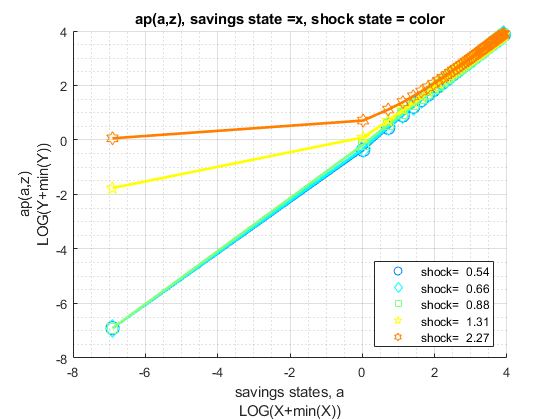
\includegraphics[width=5.20833in,height=\textheight]{img/fx_vfi_az_bisec_loop_images/figure_1.png}

Run the function and show summaries for savings and fraction of coh
saved:

\begin{verbatim}
mp_params('it_a_n') = 100;
mp_params('it_z_n') = 9;
mp_support('ls_ffcmd') = {'ap', 'savefraccoh'};
mp_support('ls_ffsna') = {};
mp_support('ls_ffgrh') = {};
mp_support('bl_vfi_store_all') = true; % store c(a,z), y(a,z)
ff_vfi_az_bisec_loop(mp_params, mp_support);

Elapsed time is 57.010652 seconds.
----------------------------------------
xxxxxxxxxxxxxxxxxxxxxxxxxxxxxxxxxxxxxxxx
CONTAINER NAME: mp_ffcmd ND Array (Matrix etc)
xxxxxxxxxxxxxxxxxxxxxxxxxxxxxxxxxxxxxxxx
                   i    idx    ndim    numel    rowN    colN     sum       mean        std      coefvari    min      max  
                   _    ___    ____    _____    ____    ____    ______    _______    _______    ________    ___    _______

    ap             1     1      2       900     100      9       12926     14.362     14.544     1.0127      0      51.171
    savefraccoh    2     2      2       900     100      9      621.24    0.69027    0.26896    0.38965      0     0.92739

xxx TABLE:ap xxxxxxxxxxxxxxxxxx
              c1        c2        c3          c4           c5         c6         c7         c8        c9  
            ______    ______    ______    __________    ________    _______    _______    ______    ______

    r1           0         0         0             0    0.087442    0.27778    0.58243    1.0038    1.5724
    r2           0         0         0             0    0.087962    0.27828    0.58297    1.0044    1.5731
    r3           0         0         0             0    0.090477    0.28074    0.58547    1.0069    1.5755
    r4           0         0         0    0.00055771     0.09279    0.28605     0.5907    1.0122    1.5808
    r5           0         0         0     0.0059496     0.09602    0.29477    0.59952    1.0209    1.5895
    r96     43.845    43.923    44.022        44.198      44.428     44.722     45.103    45.546    46.186
    r97     45.031    45.101    45.208        45.384      45.613      45.91     46.293    46.735    47.382
    r98     46.237    46.297    46.411         46.59      46.818     47.115     47.501    47.948    48.605
    r99      47.46    47.512    47.635        47.812      48.041      48.34     48.726    49.191    49.869
    r100    48.703    48.746    48.878        49.055      49.283     49.586     49.978    50.495    51.171

xxx TABLE:savefraccoh xxxxxxxxxxxxxxxxxx
              c1         c2         c3           c4           c5         c6         c7         c8         c9   
            _______    _______    _______    __________    ________    _______    _______    _______    _______

    r1            0          0          0             0    0.066018    0.16569    0.27445    0.37369    0.46243
    r2            0          0          0             0    0.066384    0.16593    0.27463    0.37381    0.46256
    r3            0          0          0             0    0.068154    0.16715    0.27549    0.37442    0.46292
    r4            0          0          0    0.00052879    0.069619    0.16978    0.27726    0.37564    0.46378
    r5            0          0          0     0.0055946    0.071572    0.17405    0.28025    0.37766    0.46512
    r96     0.92458    0.92354    0.92226       0.92171     0.92116    0.92055    0.91994    0.91842    0.91811
    r97     0.92531    0.92416    0.92306       0.92251     0.92196    0.92141    0.92086    0.91933    0.91915
    r98     0.92605     0.9247    0.92379        0.9233     0.92275     0.9222    0.92171    0.92031    0.92031
    r99     0.92672    0.92525    0.92452       0.92403     0.92348      0.923    0.92251    0.92147    0.92184
    r100    0.92739     0.9258    0.92525       0.92477     0.92422    0.92379    0.92342    0.92336    0.92367
\end{verbatim}

\hypertarget{test-ff_vfi_az_bisec_loop-change-interest-rate-and-discount}{%
\subsection{Test FF\_VFI\_AZ\_BISEC\_LOOP Change Interest Rate and Discount}\label{test-ff_vfi_az_bisec_loop-change-interest-rate-and-discount}}

Show only save fraction of cash on hand:

\begin{verbatim}
mp_support = containers.Map('KeyType','char', 'ValueType','any');
mp_support('bl_print_params') = false;
mp_support('bl_print_iterinfo') = false;
mp_support('ls_ffcmd') = {'savefraccoh'};
mp_support('ls_ffsna') = {};
mp_support('ls_ffgrh') = {};
mp_params = containers.Map('KeyType','char', 'ValueType','any');
mp_params('it_a_n') = 100;
mp_params('it_z_n') = 7;
mp_params('fl_a_max') = 50;
mp_params('st_grid_type') = 'grid_powerspace';
\end{verbatim}

Solve the model with several different interest rates and discount
factor:

\begin{verbatim}
% Lower Savings Incentives
mp_params('fl_beta') = 0.80;
mp_params('fl_r') = 0.01;
ff_vfi_az_bisec_loop(mp_params, mp_support);

Elapsed time is 10.824225 seconds.
----------------------------------------
xxxxxxxxxxxxxxxxxxxxxxxxxxxxxxxxxxxxxxxx
CONTAINER NAME: mp_ffcmd ND Array (Matrix etc)
xxxxxxxxxxxxxxxxxxxxxxxxxxxxxxxxxxxxxxxx
                   i    idx    ndim    numel    rowN    colN     sum       mean        std      coefvari    min      max  
                   _    ___    ____    _____    ____    ____    ______    _______    _______    ________    ___    _______

    savefraccoh    1     1      2       700     100      7      357.85    0.51122    0.27528    0.53848      0     0.79965

xxx TABLE:savefraccoh xxxxxxxxxxxxxxxxxx
              c1         c2         c3         c4         c5           c6           c7   
            _______    _______    _______    _______    _______    __________    ________

    r1            0          0          0          0          0    0.00022362    0.041544
    r2            0          0          0          0          0    0.00022362    0.041544
    r3            0          0          0          0          0     0.0011391    0.041544
    r4            0          0          0          0          0     0.0016884    0.041483
    r5            0          0          0          0          0     0.0034584     0.04136
    r96     0.79586    0.79275    0.78945    0.78591    0.78225       0.77853     0.77059
    r97     0.79684    0.79379    0.79055    0.78713    0.78359       0.77993     0.77212
    r98     0.79782    0.79482    0.79171    0.78835    0.78488       0.78127     0.77365
    r99     0.79873    0.79586    0.79275    0.78951     0.7861       0.78262     0.77548
    r100    0.79965    0.79684    0.79385    0.79061    0.78732        0.7839      0.7781

% Higher Savings Incentives
mp_params('fl_beta') = 0.95;
mp_params('fl_r') = 0.04;
ff_vfi_az_bisec_loop(mp_params, mp_support);

Elapsed time is 53.369195 seconds.
----------------------------------------
xxxxxxxxxxxxxxxxxxxxxxxxxxxxxxxxxxxxxxxx
CONTAINER NAME: mp_ffcmd ND Array (Matrix etc)
xxxxxxxxxxxxxxxxxxxxxxxxxxxxxxxxxxxxxxxx
                   i    idx    ndim    numel    rowN    colN     sum       mean        std      coefvari    min      max  
                   _    ___    ____    _____    ____    ____    ______    _______    _______    ________    ___    _______

    savefraccoh    1     1      2       700     100      7      481.37    0.68768    0.27118    0.39435      0     0.92702

xxx TABLE:savefraccoh xxxxxxxxxxxxxxxxxx
              c1         c2         c3          c4         c5         c6         c7   
            _______    _______    _______    ________    _______    _______    _______

    r1            0          0          0    0.065774    0.18076    0.30655    0.41654
    r2            0          0          0    0.066201    0.18101    0.30674     0.4166
    r3            0          0          0     0.06791    0.18223    0.30747    0.41709
    r4            0          0          0    0.069619    0.18467    0.30759    0.41812
    r5            0          0          0    0.071694    0.18876    0.30838    0.41983
    r96     0.92428    0.92245    0.92178     0.92116    0.92049    0.91872    0.91824
    r97     0.92501    0.92324    0.92257     0.92196    0.92129    0.91958    0.91921
    r98     0.92574    0.92397    0.92336     0.92275    0.92208    0.92049    0.92025
    r99     0.92647     0.9247    0.92409     0.92348    0.92287    0.92147    0.92159
    r100    0.92702    0.92544    0.92483     0.92422    0.92373    0.92336    0.92348
\end{verbatim}

\hypertarget{test-ff_vfi_az_bisec_loop-changing-risk-aversion}{%
\subsection{Test FF\_VFI\_AZ\_BISEC\_LOOP Changing Risk Aversion}\label{test-ff_vfi_az_bisec_loop-changing-risk-aversion}}

Here, again, show fraction of coh saved in summary tabular form, but
also show it graphically.

\begin{verbatim}
mp_support = containers.Map('KeyType','char', 'ValueType','any');
mp_support('bl_print_params') = false;
mp_support('bl_print_iterinfo') = false;
mp_support('ls_ffcmd') = {'savefraccoh'};
mp_support('ls_ffsna') = {};
mp_support('ls_ffgrh') = {'savefraccoh'};
mp_params = containers.Map('KeyType','char', 'ValueType','any');
mp_params('it_a_n') = 100;
mp_params('it_z_n') = 7;
mp_params('fl_a_max') = 50;
mp_params('st_grid_type') = 'grid_powerspace';
\end{verbatim}

Solve the model with different risk aversion levels, higher preferences
for risk:

\begin{verbatim}
% Lower Risk Aversion
mp_params('fl_crra') = 0.5;
ff_vfi_az_bisec_loop(mp_params, mp_support);

Elapsed time is 47.635241 seconds.
----------------------------------------
xxxxxxxxxxxxxxxxxxxxxxxxxxxxxxxxxxxxxxxx
CONTAINER NAME: mp_ffcmd ND Array (Matrix etc)
xxxxxxxxxxxxxxxxxxxxxxxxxxxxxxxxxxxxxxxx
                   i    idx    ndim    numel    rowN    colN     sum       mean       std      coefvari    min      max  
                   _    ___    ____    _____    ____    ____    ______    ______    _______    ________    ___    _______

    savefraccoh    1     1      2       700     100      7      452.13    0.6459    0.28031    0.43398      0     0.90359

xxx TABLE:savefraccoh xxxxxxxxxxxxxxxxxx
              c1         c2         c3          c4           c5         c6         c7   
            _______    _______    _______    _________    ________    _______    _______

    r1            0          0          0    0.0047401    0.089089    0.19822    0.30783
    r2            0          0          0    0.0051674    0.089394     0.1984    0.30796
    r3            0          0          0    0.0060218    0.090676    0.19926    0.30851
    r4            0          0          0    0.0082801    0.092812    0.20115    0.30973
    r5            0          0          0     0.012247    0.092995     0.2042    0.31174
    r96     0.90047    0.89925    0.89828       0.8973     0.89632    0.89376    0.89297
    r97     0.90127    0.90017    0.89919      0.89828      0.8973     0.8948    0.89394
    r98     0.90206    0.90102    0.90011      0.89919     0.89828    0.89577    0.89498
    r99     0.90279    0.90188    0.90102      0.90011     0.89919    0.89681     0.8959
    r100    0.90359    0.90273    0.90188      0.90096     0.90011    0.89803    0.89687
\end{verbatim}

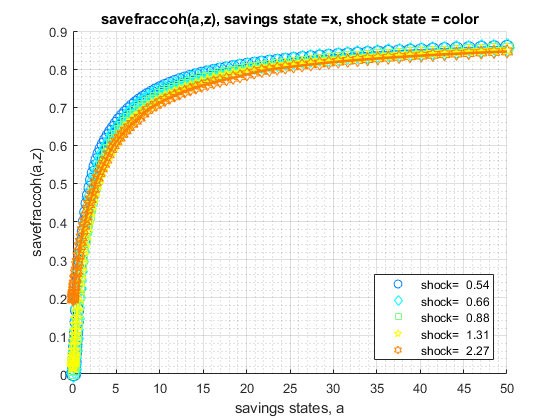
\includegraphics[width=5.20833in,height=\textheight]{img/fx_vfi_az_bisec_loop_images/figure_2.png}

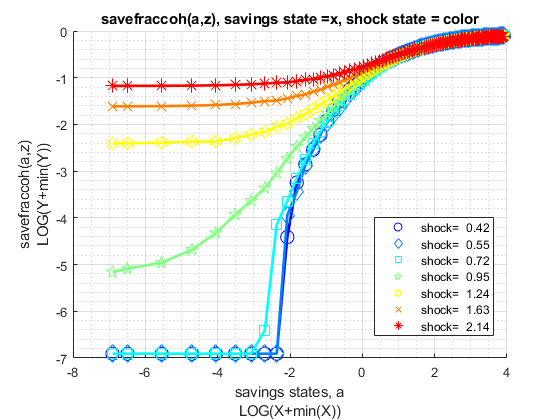
\includegraphics[width=5.20833in,height=\textheight]{img/fx_vfi_az_bisec_loop_images/figure_3.png}

When risk aversion increases, at every state-space point, the household
wants to save more.

\begin{verbatim}
% Higher Risk Aversion
mp_params('fl_crra') = 5;
ff_vfi_az_bisec_loop(mp_params, mp_support);

Elapsed time is 46.937845 seconds.
----------------------------------------
xxxxxxxxxxxxxxxxxxxxxxxxxxxxxxxxxxxxxxxx
CONTAINER NAME: mp_ffcmd ND Array (Matrix etc)
xxxxxxxxxxxxxxxxxxxxxxxxxxxxxxxxxxxxxxxx
                   i    idx    ndim    numel    rowN    colN     sum       mean        std      coefvari    min      max  
                   _    ___    ____    _____    ____    ____    ______    _______    _______    ________    ___    _______

    savefraccoh    1     1      2       700     100      7      502.71    0.71816    0.25437     0.3542      0     0.93587

xxx TABLE:savefraccoh xxxxxxxxxxxxxxxxxx
              c1         c2          c3         c4         c5         c6         c7   
            _______    _______    ________    _______    _______    _______    _______

    r1            0          0    0.047037    0.15537    0.27573     0.3909    0.48782
    r2            0          0    0.047525    0.15531    0.27591    0.39102    0.48795
    r3            0          0    0.049844     0.1569    0.27695     0.3917    0.48837
    r4            0          0    0.054788    0.16025    0.27915     0.3931    0.48929
    r5            0          0    0.062905    0.16569    0.28275    0.39542    0.49075
    r96     0.93307    0.93258     0.93203    0.93154     0.9302    0.92995    0.92971
    r97     0.93374    0.93325     0.93276    0.93227    0.93111    0.93105    0.93117
    r98     0.93441    0.93398     0.93349    0.93307    0.93209    0.93227     0.9327
    r99     0.93508    0.93465     0.93423    0.93392    0.93331    0.93368    0.93435
    r100    0.93575    0.93539     0.93508     0.9349    0.93496    0.93526    0.93587
\end{verbatim}

\includegraphics[width=5.20833in,height=\textheight]{img/fx_vfi_az_bisec_loop_images/figure_4.png}

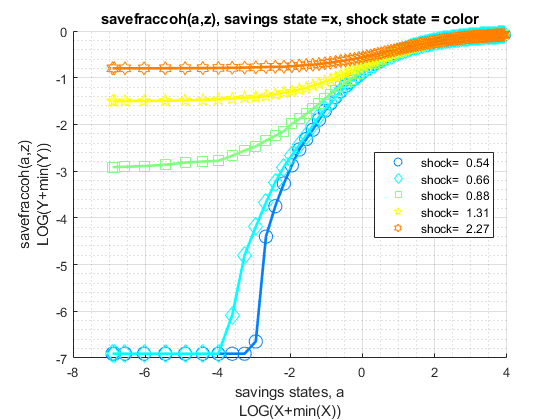
\includegraphics[width=5.20833in,height=\textheight]{img/fx_vfi_az_bisec_loop_images/figure_5.png}

\hypertarget{test-ff_vfi_az_bisec_loop-with-higher-uncertainty}{%
\subsection{Test FF\_VFI\_AZ\_BISEC\_LOOP with Higher Uncertainty}\label{test-ff_vfi_az_bisec_loop-with-higher-uncertainty}}

Increase the standard deviation of the Shock.

\begin{verbatim}
mp_support = containers.Map('KeyType','char', 'ValueType','any');
mp_support('bl_print_params') = false;
mp_support('bl_print_iterinfo') = false;
mp_support('ls_ffcmd') = {'savefraccoh'};
mp_support('ls_ffsna') = {};
mp_support('ls_ffgrh') = {};
mp_params = containers.Map('KeyType','char', 'ValueType','any');
mp_params('it_a_n') = 150;
mp_params('it_z_n') = 15;
mp_params('fl_a_max') = 50;
mp_params('st_grid_type') = 'grid_powerspace';
% graph color spectrum
mp_params('cl_colors') = 'copper';
\end{verbatim}

Lower standard deviation of shock:

\begin{verbatim}
% Lower Risk Aversion
mp_params('fl_shk_std') = 0.10;
ff_vfi_az_bisec_loop(mp_params, mp_support);

Elapsed time is 150.979328 seconds.
----------------------------------------
xxxxxxxxxxxxxxxxxxxxxxxxxxxxxxxxxxxxxxxx
CONTAINER NAME: mp_ffcmd ND Array (Matrix etc)
xxxxxxxxxxxxxxxxxxxxxxxxxxxxxxxxxxxxxxxx
                   i    idx    ndim    numel    rowN    colN     sum       mean        std      coefvari    min      max  
                   _    ___    ____    _____    ____    ____    ______    _______    _______    ________    ___    _______

    savefraccoh    1     1      2      2250     150      15     1507.5    0.67001    0.28668    0.42788      0     0.92568

xxx TABLE:savefraccoh xxxxxxxxxxxxxxxxxx
              c1         c2         c3         c4         c5         c11        c12        c13        c14        c15  
            _______    _______    _______    _______    _______    _______    _______    _______    _______    _______

    r1            0          0          0          0          0    0.13847    0.18485    0.23026    0.27378    0.31729
    r2            0          0          0          0          0    0.13853    0.18491    0.23032    0.27384    0.31736
    r3            0          0          0          0          0    0.13895    0.18528    0.23063    0.27408     0.3176
    r4            0          0          0          0          0    0.13987    0.18607     0.2313    0.27469    0.31809
    r5            0          0          0          0          0    0.14011    0.18735     0.2324    0.27567    0.31888
    r146    0.92373    0.92354     0.9233    0.92312    0.92287    0.92086    0.92068    0.92049    0.91952    0.91933
    r147    0.92422    0.92403    0.92385    0.92361    0.92342    0.92141    0.92123    0.92098    0.92007    0.91988
    r148     0.9247    0.92452    0.92434    0.92409    0.92391     0.9219    0.92171    0.92153    0.92062    0.92043
    r149    0.92519    0.92501    0.92483    0.92458     0.9244    0.92245    0.92226    0.92208    0.92116     0.9211
    r150    0.92568     0.9255    0.92531    0.92507    0.92489    0.92293    0.92275    0.92257    0.92245    0.92232
\end{verbatim}

Higher shock standard deviation: low shock high asset save more, high
shock more asset save less, high shock low asset save more:

\begin{verbatim}
% Higher Risk Aversion
mp_params('fl_shk_std') = 0.40;
ff_vfi_az_bisec_loop(mp_params, mp_support);

Elapsed time is 136.803951 seconds.
----------------------------------------
xxxxxxxxxxxxxxxxxxxxxxxxxxxxxxxxxxxxxxxx
CONTAINER NAME: mp_ffcmd ND Array (Matrix etc)
xxxxxxxxxxxxxxxxxxxxxxxxxxxxxxxxxxxxxxxx
                   i    idx    ndim    numel    rowN    colN     sum       mean        std      coefvari    min      max  
                   _    ___    ____    _____    ____    ____    ______    _______    _______    ________    ___    _______

    savefraccoh    1     1      2      2250     150      15     1685.6    0.74914    0.22909     0.3058      0     0.93679

xxx TABLE:savefraccoh xxxxxxxxxxxxxxxxxx
              c1         c2         c3         c4         c5         c11        c12        c13        c14        c15  
            _______    _______    _______    _______    _______    _______    _______    _______    _______    _______

    r1            0          0          0          0          0     0.5264    0.61264    0.68271    0.73922    0.78433
    r2            0          0          0          0          0    0.52646    0.61264    0.68271    0.73922    0.78433
    r3            0          0          0          0          0    0.52658     0.6127    0.68271    0.73922    0.78433
    r4            0          0          0          0          0    0.52682    0.61288    0.68283    0.73928    0.78439
    r5            0          0          0          0          0    0.52731    0.61313    0.68295    0.73934    0.78439
    r146    0.92983    0.92928    0.92873    0.92806    0.92739    0.92269    0.92354     0.9258    0.92904    0.93331
    r147     0.9302    0.92971     0.9291    0.92849    0.92788    0.92361    0.92477     0.9269    0.93001    0.93423
    r148    0.93056    0.93008    0.92953    0.92892    0.92831    0.92458    0.92593      0.928    0.93105    0.93508
    r149    0.93093    0.93044    0.92995    0.92934    0.92873     0.9258    0.92702     0.9291    0.93203      0.936
    r150     0.9313    0.93087    0.93032    0.92977    0.92916    0.92696    0.92818    0.93014    0.93294    0.93679
\end{verbatim}

\hypertarget{ff_vfi_az_bisec_vec-savings-vectorized-exact-foc-examples}{%
\section{FF\_VFI\_AZ\_BISEC\_VEC Savings Vectorized Exact (FOC) Examples}\label{ff_vfi_az_bisec_vec-savings-vectorized-exact-foc-examples}}

\begin{quote}
Go back to \href{http://fanwangecon.github.io/}{fan}'s \href{https://fanwangecon.github.io/MEconTools/}{MEconTools} Toolbox (\href{https://fanwangecon.github.io/MEconTools/bookdown}{bookdown}), \href{https://fanwangecon.github.io/M4Econ/}{Matlab Code Examples} Repository (\href{https://fanwangecon.github.io/M4Econ/bookdown}{bookdown}), or \href{https://fanwangecon.github.io/Math4Econ/}{Math for Econ with Matlab} Repository (\href{https://fanwangecon.github.io/Math4Econ/bookdown}{bookdown}).
\end{quote}

This is the example vignette for function:
\href{https://github.com/FanWangEcon/MEconTools/blob/master/MEconTools/vfi/ff_vfi_az_bisec_vec.m}{\textbf{ff\_vfi\_az\_bisec\_vec}}
from the \href{https://fanwangecon.github.io/MEconTools/}{\textbf{MEconTools
Package}}\textbf{.} This function
solves the dynamic programming problem for a (a,z) model. Households can
save a, and face AR(1) shock z. The problem is solved over the infinite
horizon.

This is the vectorized code, its speed is much faster than the looped
code. The function is designed to have small memory footprint and
requires low computing resources, yet is fast.

The code uses \textbf{continuous choices}, solved with bi(multi)section. The
state-space is on a grid, but choice grids are in terms of percentage of
resources available, which is individual specific, to save and solved
exactly up to ((1/(2)\^{}16)*100=0.001525878) percentage of cash on hand.
The
\href{https://github.com/FanWangEcon/MEconTools/blob/master/MEconTools/vfi/ff_vfi_az_vec.m}{\textbf{ff\_vfi\_az\_vec}}
from the \href{https://fanwangecon.github.io/MEconTools/}{\textbf{MEconTools
Package}} solves the same
problem using vectorized common grid code where the choice set and state
space share the same grid. The common grid function is faster, but less
precise for the same number of asset grid points.

\textbf{Links to Other Code:}

Core Savings/Borrowing Dynamic Programming Solution Functions that are
functions in the \href{https://fanwangecon.github.io/MEconTools/}{\textbf{MEconTools
Package}}\textbf{.} :

\begin{itemize}
\item
  Common Choice and States Grid :
  \href{https://github.com/FanWangEcon/MEconTools/blob/master/MEconTools/vfi/ff_vfi_az_loop.m}{\textbf{ff\_vfi\_az\_loop}}
\item
  Common Choice and States Grid :
  \href{https://github.com/FanWangEcon/MEconTools/blob/master/MEconTools/vfi/ff_vfi_az_vec.m}{\textbf{ff\_vfi\_az\_vec}}
\item
  States Grid + Continuous Exact Savings as Share of Cash-on-Hand,
  rely on FOC, :\href{https://github.com/FanWangEcon/MEconTools/blob/master/MEconTools/vfi/ff_vfi_az_bisec_loop.m}{\textbf{ff\_vfi\_az\_bisec\_loop}}
\item
  States Grid + Continuous Exact Savings as Share of Cash-on-Hand,
  rely on FOC :
  \href{https://github.com/FanWangEcon/MEconTools/blob/master/MEconTools/vfi/ff_vfi_az_bisec_vec.m}{\textbf{ff\_vfi\_az\_bisec\_vec}}
\item
  States Grid + Continuous Exact Savings as Share of Cash-on-Hand,
  VALUE comparison, :\href{https://github.com/FanWangEcon/MEconTools/blob/master/MEconTools/vfi/ff_vfi_az_mzoom_loop.m}{\textbf{ff\_vfi\_az\_mzoom\_loop}}
\item
  States Grid + Continuous Exact Savings as Share of Cash-on-Hand,
  VALUE comparison, :
  \href{https://github.com/FanWangEcon/MEconTools/blob/master/MEconTools/vfi/ff_vfi_az_mzoom_vec.m}{\textbf{ff\_vfi\_az\_mzoom\_vec}}
\end{itemize}

\hypertarget{test-ff_vfi_az_bisec_vec-defaults}{%
\subsection{Test FF\_VFI\_AZ\_BISEC\_VEC Defaults}\label{test-ff_vfi_az_bisec_vec-defaults}}

Call the function with defaults. By default, shows the asset policy
function summary. Model parameters can be changed by the mp\_params.

\begin{verbatim}
%mp_params
mp_params = containers.Map('KeyType','char', 'ValueType','any');
mp_params('fl_crra') = 1.5;
mp_params('fl_beta') = 0.94;
% call function
ff_vfi_az_bisec_vec(mp_params);

Elapsed time is 1.762201 seconds.
----------------------------------------
xxxxxxxxxxxxxxxxxxxxxxxxxxxxxxxxxxxxxxxx
CONTAINER NAME: mp_ffcmd ND Array (Matrix etc)
xxxxxxxxxxxxxxxxxxxxxxxxxxxxxxxxxxxxxxxx
          i    idx    ndim    numel    rowN    colN     sum       mean      std      coefvari    min     max  
          _    ___    ____    _____    ____    ____    ______    ______    ______    ________    ___    ______

    ap    1     1      2       700     100      7      9863.4    14.091    14.388     1.0211      0     50.117

xxx TABLE:ap xxxxxxxxxxxxxxxxxx
              c1        c2        c3         c4         c5         c6         c7  
            ______    ______    ______    ________    _______    _______    ______

    r1           0         0         0    0.053491    0.25574    0.60604    1.1157
    r2           0         0         0    0.053998    0.25571     0.6066    1.1163
    r3           0         0         0    0.056449    0.25576    0.60907    1.1187
    r4           0         0         0    0.061799    0.26016     0.6109    1.1239
    r5           0         0         0    0.066463    0.26897    0.61141    1.1327
    r96     43.388     43.52    43.701      43.925     44.222      44.68    45.228
    r97     44.566    44.695    44.878      45.103     45.398     45.856    46.403
    r98     45.761    45.892    46.072      46.298     46.592      47.05    47.597
    r99     46.973    47.107    47.286      47.514     47.806     48.263    48.815
    r100    48.206    48.338    48.519      48.746     49.037     49.497    50.117
\end{verbatim}

\hypertarget{test-ff_vfi_az_bisec_vec-speed-tests-2}{%
\subsection{Test FF\_VFI\_AZ\_BISEC\_VEC Speed Tests}\label{test-ff_vfi_az_bisec_vec-speed-tests-2}}

Call the function with defaults. By default, shows the asset policy
function summary. Model parameters can be changed by the mp\_params.

\begin{verbatim}
mp_support = containers.Map('KeyType','char', 'ValueType','any');
mp_support('bl_timer') = true;
mp_support('ls_ffcmd') = {};
% A grid 50, shock grid 5:
mp_params = containers.Map('KeyType','char', 'ValueType','any');
mp_params('it_a_n') = 50;
mp_params('it_z_n') = 5;
ff_vfi_az_bisec_vec(mp_params, mp_support);

Elapsed time is 0.792541 seconds.

% A grid 750, shock grid 15:
mp_params = containers.Map('KeyType','char', 'ValueType','any');
mp_params('it_a_n') = 750;
mp_params('it_z_n') = 15;
ff_vfi_az_bisec_vec(mp_params, mp_support);

Elapsed time is 43.095190 seconds.

% A grid 600, shock grid 45:
mp_params = containers.Map('KeyType','char', 'ValueType','any');
mp_params('it_a_n') = 600;
mp_params('it_z_n') = 45;
ff_vfi_az_bisec_vec(mp_params, mp_support);

Elapsed time is 80.139775 seconds.
\end{verbatim}

\hypertarget{test-ff_vfi_az_bisec_vec-control-outputs}{%
\subsection{Test FF\_VFI\_AZ\_BISEC\_VEC Control Outputs}\label{test-ff_vfi_az_bisec_vec-control-outputs}}

Run the function first without any outputs;

\begin{verbatim}
mp_params = containers.Map('KeyType','char', 'ValueType','any');
mp_params('it_a_n') = 50;
mp_params('it_z_n') = 5;
mp_support = containers.Map('KeyType','char', 'ValueType','any');
mp_support('bl_timer') = true;
mp_support('bl_print_params') = false;
mp_support('bl_print_iterinfo') = false;
mp_support('ls_ffcmd') = {};
ff_vfi_az_vec(mp_params, mp_support);

Elapsed time is 0.029901 seconds.
\end{verbatim}

Run the function and show policy function for savings choice. For
ls\_ffcmd, ls\_ffsna, ls\_ffgrh, can include these: `v', `ap', `c', `y',
`coh', `savefraccoh'. These are value, aprime savings choice,
consumption, income, cash on hand, and savings fraction as cash-on-hand.

\begin{verbatim}
mp_support = containers.Map('KeyType','char', 'ValueType','any');
mp_support('bl_print_params') = false;
mp_support('bl_print_iterinfo') = false;
% ls_ffcmd: summary print which outcomes
mp_support('ls_ffcmd') = {};
% ls_ffsna: detail print which outcomes
mp_support('ls_ffsna') = {'savefraccoh'};
% ls_ffgrh: graphical print which outcomes
mp_support('ls_ffgrh') = {'savefraccoh'};
ff_vfi_az_bisec_vec(mp_params, mp_support);

Elapsed time is 0.494900 seconds.
xxx  ff_vfi_az_vec, outcome=savefraccoh  xxxxxxxxxxxxxxxxxxxxxxxxxxx
    group       a        mean_z_0_4858    mean_z_0_67798    mean_z_0_9462    mean_z_1_3205    mean_z_1_8429
    _____    ________    _____________    ______________    _____________    _____________    _____________

      1             0              0                0         0.067239          0.20859          0.35953   
      2      0.002975              0                0         0.069375          0.20829          0.36032   
      3      0.016829              0                0         0.070901           0.2139          0.36215   
      4      0.046375              0        0.0061439         0.087319           0.2266          0.36264   
      5      0.095198      0.0087684         0.034403           0.1168           0.2468          0.37473   
      6        0.1663       0.054361         0.077248           0.1522          0.26639          0.39151   
      7       0.26234       0.099892          0.13132          0.19388          0.29929          0.41281   
      8       0.38568        0.15958          0.19309          0.24112          0.33017          0.43088   
      9       0.53852        0.23417          0.25553          0.29215          0.37436          0.45969   
     10       0.72291         0.3071          0.31656          0.34812          0.41153          0.48386   
     11       0.94076        0.37595          0.37503          0.40842          0.44925          0.50992   
     12        1.1939        0.43881          0.42941          0.45755          0.48697          0.54367   
     13         1.484        0.49509          0.48129          0.50381          0.53262          0.56979   
     14        1.8128        0.54489          0.53018          0.54642          0.56778          0.59634   
     15        2.1817        0.58871          0.57382          0.58548          0.60055           0.6282   
     16        2.5924        0.62716          0.61258          0.62076          0.63101          0.65249   
     17        3.0463        0.66079          0.64682          0.65243          0.65884           0.6752   
     18        3.5449        0.69027          0.67709          0.68069          0.68423          0.69638   
     19        4.0894        0.71621          0.70376          0.70596          0.70724          0.71591   
     20        4.6813        0.73703          0.72732          0.72848          0.72799          0.73385   
     21        5.3218        0.75326          0.74813           0.7485          0.74673          0.75021   
     22        6.0121        0.76913          0.76657          0.76632          0.76364          0.76535   
     23        6.7536        0.78536          0.78286          0.78231          0.77889           0.7842   
     24        7.5474        0.79983          0.79745          0.79653          0.79269          0.79678   
     25        8.3948        0.81271          0.81039          0.80929          0.80514          0.80831   
     26        9.2967        0.82418          0.82198          0.82076          0.81637          0.81875   
     27        10.254         0.8345          0.83242          0.83114          0.82656          0.82833   
     28        11.269        0.84377          0.84176          0.84042          0.83584          0.83706   
     29        12.342        0.85214          0.85024          0.84884           0.8442          0.84499   
     30        13.473        0.85964          0.85781          0.85647          0.85183          0.85232   
     31        14.665        0.86648          0.86471          0.86337          0.85879          0.85897   
     32        15.918        0.87264          0.87099          0.86965          0.86507          0.86507   
     33        17.233        0.87826          0.87667          0.87533          0.87161          0.87063   
     34        18.611        0.88338          0.88186          0.88052          0.87771          0.87582   
     35        20.053        0.88802          0.88656          0.88528          0.88326          0.88052   
     36         21.56         0.8923          0.89089          0.88967          0.88833          0.88485   
     37        23.133        0.89614          0.89486          0.89364           0.8926          0.88888   
     38        24.773        0.89974          0.89852           0.8973          0.89626           0.8926   
     39        26.481        0.90304          0.90182          0.90072          0.89968          0.89608   
     40        28.258        0.90603          0.90493          0.90383          0.90279          0.89925   
     41        30.104        0.90884          0.90774           0.9067          0.90572          0.90218   
     42        32.021         0.9114          0.91036          0.90932          0.90841          0.90493   
     43         34.01        0.91378           0.9128          0.91183          0.91091          0.90749   
     44         36.07        0.91598          0.91506          0.91408          0.91317          0.90987   
     45        38.204        0.91805          0.91714          0.91622          0.91537          0.91207   
     46        40.412        0.91994          0.91909          0.91817          0.91732          0.91415   
     47        42.695        0.92171          0.92086          0.92001          0.91921           0.9161   
     48        45.053        0.92336          0.92257          0.92171          0.92092          0.91799   
     49        47.488        0.92489          0.92409          0.92336          0.92257          0.92025   
     50            50        0.92629          0.92562          0.92489          0.92428          0.92403   
\end{verbatim}

\includegraphics[width=5.20833in,height=\textheight]{img/fx_vfi_az_bisec_vec_images/figure_0.png}

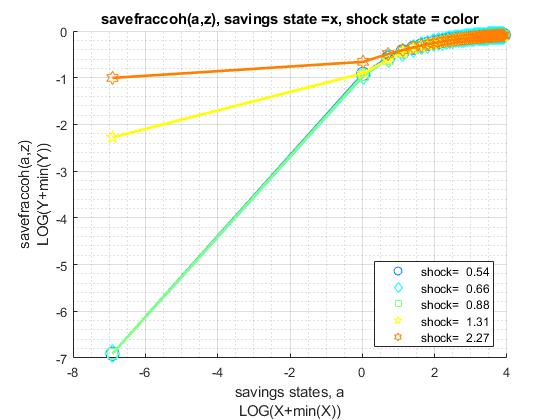
\includegraphics[width=5.20833in,height=\textheight]{img/fx_vfi_az_bisec_vec_images/figure_1.png}

Run the function and show summaries for savings and fraction of coh
saved:

\begin{verbatim}
mp_params('it_a_n') = 100;
mp_params('it_z_n') = 9;
mp_support('ls_ffcmd') = {'ap', 'savefraccoh'};
mp_support('ls_ffsna') = {};
mp_support('ls_ffgrh') = {};
mp_support('bl_vfi_store_all') = true; % store c(a,z), y(a,z)
ff_vfi_az_bisec_vec(mp_params, mp_support);

Elapsed time is 1.164186 seconds.
----------------------------------------
xxxxxxxxxxxxxxxxxxxxxxxxxxxxxxxxxxxxxxxx
CONTAINER NAME: mp_ffcmd ND Array (Matrix etc)
xxxxxxxxxxxxxxxxxxxxxxxxxxxxxxxxxxxxxxxx
                   i    idx    ndim    numel    rowN    colN     sum       mean        std      coefvari    min      max  
                   _    ___    ____    _____    ____    ____    ______    _______    _______    ________    ___    _______

    ap             1     1      2       900     100      9       12926     14.362     14.544     1.0127      0      51.171
    savefraccoh    2     2      2       900     100      9      621.24    0.69027    0.26896    0.38965      0     0.92739

xxx TABLE:ap xxxxxxxxxxxxxxxxxx
              c1        c2        c3          c4           c5         c6         c7         c8        c9  
            ______    ______    ______    __________    ________    _______    _______    ______    ______

    r1           0         0         0             0    0.087442    0.27778    0.58243    1.0038    1.5724
    r2           0         0         0             0    0.087962    0.27828    0.58297    1.0044    1.5731
    r3           0         0         0             0    0.090477    0.28074    0.58547    1.0069    1.5755
    r4           0         0         0    0.00055771     0.09279    0.28605     0.5907    1.0122    1.5808
    r5           0         0         0     0.0059496     0.09602    0.29477    0.59952    1.0209    1.5895
    r96     43.845    43.923    44.022        44.198      44.428     44.722     45.103    45.546    46.186
    r97     45.031    45.101    45.208        45.384      45.613      45.91     46.293    46.735    47.382
    r98     46.237    46.297    46.411         46.59      46.818     47.115     47.501    47.948    48.605
    r99      47.46    47.512    47.635        47.812      48.041      48.34     48.726    49.191    49.869
    r100    48.703    48.746    48.878        49.055      49.283     49.586     49.978    50.495    51.171

xxx TABLE:savefraccoh xxxxxxxxxxxxxxxxxx
              c1         c2         c3           c4           c5         c6         c7         c8         c9   
            _______    _______    _______    __________    ________    _______    _______    _______    _______

    r1            0          0          0             0    0.066018    0.16569    0.27445    0.37369    0.46243
    r2            0          0          0             0    0.066384    0.16593    0.27463    0.37381    0.46256
    r3            0          0          0             0    0.068154    0.16715    0.27549    0.37442    0.46292
    r4            0          0          0    0.00052879    0.069619    0.16978    0.27726    0.37564    0.46378
    r5            0          0          0     0.0055946    0.071572    0.17405    0.28025    0.37766    0.46512
    r96     0.92458    0.92354    0.92226       0.92171     0.92116    0.92055    0.91994    0.91842    0.91811
    r97     0.92531    0.92416    0.92306       0.92251     0.92196    0.92141    0.92086    0.91933    0.91915
    r98     0.92605     0.9247    0.92379        0.9233     0.92275     0.9222    0.92171    0.92031    0.92031
    r99     0.92672    0.92525    0.92452       0.92403     0.92348      0.923    0.92251    0.92147    0.92184
    r100    0.92739     0.9258    0.92525       0.92477     0.92422    0.92379    0.92342    0.92336    0.92367
\end{verbatim}

\hypertarget{test-ff_vfi_az_bisec_vec-change-interest-rate-and-discount}{%
\subsection{Test FF\_VFI\_AZ\_BISEC\_VEC Change Interest Rate and Discount}\label{test-ff_vfi_az_bisec_vec-change-interest-rate-and-discount}}

Show only save fraction of cash on hand:

\begin{verbatim}
mp_support = containers.Map('KeyType','char', 'ValueType','any');
mp_support('bl_print_params') = false;
mp_support('bl_print_iterinfo') = false;
mp_support('ls_ffcmd') = {'savefraccoh'};
mp_support('ls_ffsna') = {};
mp_support('ls_ffgrh') = {};
mp_params = containers.Map('KeyType','char', 'ValueType','any');
mp_params('it_a_n') = 100;
mp_params('it_z_n') = 7;
mp_params('fl_a_max') = 50;
mp_params('st_grid_type') = 'grid_powerspace';
\end{verbatim}

Solve the model with several different interest rates and discount
factor:

\begin{verbatim}
% Lower Savings Incentives
mp_params('fl_beta') = 0.80;
mp_params('fl_r') = 0.01;
ff_vfi_az_bisec_vec(mp_params, mp_support);

Elapsed time is 0.271658 seconds.
----------------------------------------
xxxxxxxxxxxxxxxxxxxxxxxxxxxxxxxxxxxxxxxx
CONTAINER NAME: mp_ffcmd ND Array (Matrix etc)
xxxxxxxxxxxxxxxxxxxxxxxxxxxxxxxxxxxxxxxx
                   i    idx    ndim    numel    rowN    colN     sum       mean        std      coefvari    min      max  
                   _    ___    ____    _____    ____    ____    ______    _______    _______    ________    ___    _______

    savefraccoh    1     1      2       700     100      7      357.85    0.51122    0.27528    0.53848      0     0.79965

xxx TABLE:savefraccoh xxxxxxxxxxxxxxxxxx
              c1         c2         c3         c4         c5           c6           c7   
            _______    _______    _______    _______    _______    __________    ________

    r1            0          0          0          0          0    0.00022362    0.041544
    r2            0          0          0          0          0    0.00022362    0.041544
    r3            0          0          0          0          0     0.0011391    0.041544
    r4            0          0          0          0          0     0.0016884    0.041483
    r5            0          0          0          0          0     0.0034584     0.04136
    r96     0.79586    0.79275    0.78945    0.78591    0.78225       0.77853     0.77059
    r97     0.79684    0.79379    0.79055    0.78713    0.78359       0.77993     0.77212
    r98     0.79782    0.79482    0.79171    0.78835    0.78488       0.78127     0.77365
    r99     0.79873    0.79586    0.79275    0.78951     0.7861       0.78262     0.77548
    r100    0.79965    0.79684    0.79385    0.79061    0.78732        0.7839      0.7781

% Higher Savings Incentives
mp_params('fl_beta') = 0.95;
mp_params('fl_r') = 0.04;
ff_vfi_az_bisec_vec(mp_params, mp_support);

Elapsed time is 0.971218 seconds.
----------------------------------------
xxxxxxxxxxxxxxxxxxxxxxxxxxxxxxxxxxxxxxxx
CONTAINER NAME: mp_ffcmd ND Array (Matrix etc)
xxxxxxxxxxxxxxxxxxxxxxxxxxxxxxxxxxxxxxxx
                   i    idx    ndim    numel    rowN    colN     sum       mean        std      coefvari    min      max  
                   _    ___    ____    _____    ____    ____    ______    _______    _______    ________    ___    _______

    savefraccoh    1     1      2       700     100      7      481.37    0.68768    0.27118    0.39435      0     0.92702

xxx TABLE:savefraccoh xxxxxxxxxxxxxxxxxx
              c1         c2         c3          c4         c5         c6         c7   
            _______    _______    _______    ________    _______    _______    _______

    r1            0          0          0    0.065774    0.18076    0.30655    0.41654
    r2            0          0          0    0.066201    0.18101    0.30674     0.4166
    r3            0          0          0     0.06791    0.18223    0.30747    0.41709
    r4            0          0          0    0.069619    0.18467    0.30759    0.41812
    r5            0          0          0    0.071694    0.18876    0.30838    0.41983
    r96     0.92428    0.92245    0.92178     0.92116    0.92049    0.91872    0.91824
    r97     0.92501    0.92324    0.92257     0.92196    0.92129    0.91958    0.91921
    r98     0.92574    0.92397    0.92336     0.92275    0.92208    0.92049    0.92025
    r99     0.92647     0.9247    0.92409     0.92348    0.92287    0.92147    0.92159
    r100    0.92702    0.92544    0.92483     0.92422    0.92373    0.92336    0.92348
\end{verbatim}

\hypertarget{test-ff_vfi_az_bisec_vec-changing-risk-aversion}{%
\subsection{Test FF\_VFI\_AZ\_BISEC\_VEC Changing Risk Aversion}\label{test-ff_vfi_az_bisec_vec-changing-risk-aversion}}

Here, again, show fraction of coh saved in summary tabular form, but
also show it graphically.

\begin{verbatim}
mp_support = containers.Map('KeyType','char', 'ValueType','any');
mp_support('bl_print_params') = false;
mp_support('bl_print_iterinfo') = false;
mp_support('ls_ffcmd') = {'savefraccoh'};
mp_support('ls_ffsna') = {};
mp_support('ls_ffgrh') = {'savefraccoh'};
mp_params = containers.Map('KeyType','char', 'ValueType','any');
mp_params('it_a_n') = 100;
mp_params('it_z_n') = 7;
mp_params('fl_a_max') = 50;
mp_params('st_grid_type') = 'grid_powerspace';
\end{verbatim}

Solve the model with different risk aversion levels, higher preferences
for risk:

\begin{verbatim}
% Lower Risk Aversion
mp_params('fl_crra') = 0.5;
ff_vfi_az_bisec_vec(mp_params, mp_support);

Elapsed time is 0.873752 seconds.
----------------------------------------
xxxxxxxxxxxxxxxxxxxxxxxxxxxxxxxxxxxxxxxx
CONTAINER NAME: mp_ffcmd ND Array (Matrix etc)
xxxxxxxxxxxxxxxxxxxxxxxxxxxxxxxxxxxxxxxx
                   i    idx    ndim    numel    rowN    colN     sum       mean       std      coefvari    min      max  
                   _    ___    ____    _____    ____    ____    ______    ______    _______    ________    ___    _______

    savefraccoh    1     1      2       700     100      7      452.13    0.6459    0.28031    0.43398      0     0.90359

xxx TABLE:savefraccoh xxxxxxxxxxxxxxxxxx
              c1         c2         c3          c4           c5         c6         c7   
            _______    _______    _______    _________    ________    _______    _______

    r1            0          0          0    0.0047401    0.089089    0.19822    0.30783
    r2            0          0          0    0.0051674    0.089394     0.1984    0.30796
    r3            0          0          0    0.0060218    0.090676    0.19926    0.30851
    r4            0          0          0    0.0082801    0.092812    0.20115    0.30973
    r5            0          0          0     0.012247    0.092995     0.2042    0.31174
    r96     0.90047    0.89925    0.89828       0.8973     0.89632    0.89376    0.89297
    r97     0.90127    0.90017    0.89919      0.89828      0.8973     0.8948    0.89394
    r98     0.90206    0.90102    0.90011      0.89919     0.89828    0.89577    0.89498
    r99     0.90279    0.90188    0.90102      0.90011     0.89919    0.89681     0.8959
    r100    0.90359    0.90273    0.90188      0.90096     0.90011    0.89803    0.89687
\end{verbatim}

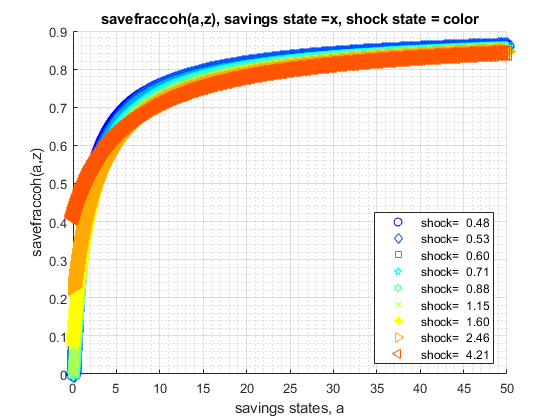
\includegraphics[width=5.20833in,height=\textheight]{img/fx_vfi_az_bisec_vec_images/figure_2.png}

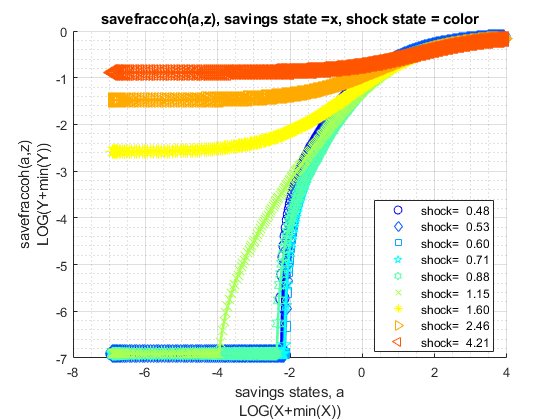
\includegraphics[width=5.20833in,height=\textheight]{img/fx_vfi_az_bisec_vec_images/figure_3.png}

When risk aversion increases, at every state-space point, the household
wants to save more.

\begin{verbatim}
% Higher Risk Aversion
mp_params('fl_crra') = 5;
ff_vfi_az_bisec_vec(mp_params, mp_support);

Elapsed time is 0.970314 seconds.
----------------------------------------
xxxxxxxxxxxxxxxxxxxxxxxxxxxxxxxxxxxxxxxx
CONTAINER NAME: mp_ffcmd ND Array (Matrix etc)
xxxxxxxxxxxxxxxxxxxxxxxxxxxxxxxxxxxxxxxx
                   i    idx    ndim    numel    rowN    colN     sum       mean        std      coefvari    min      max  
                   _    ___    ____    _____    ____    ____    ______    _______    _______    ________    ___    _______

    savefraccoh    1     1      2       700     100      7      502.71    0.71816    0.25437     0.3542      0     0.93587

xxx TABLE:savefraccoh xxxxxxxxxxxxxxxxxx
              c1         c2          c3         c4         c5         c6         c7   
            _______    _______    ________    _______    _______    _______    _______

    r1            0          0    0.047037    0.15537    0.27573     0.3909    0.48782
    r2            0          0    0.047525    0.15531    0.27591    0.39102    0.48795
    r3            0          0    0.049844     0.1569    0.27695     0.3917    0.48837
    r4            0          0    0.054788    0.16025    0.27915     0.3931    0.48929
    r5            0          0    0.062905    0.16569    0.28275    0.39542    0.49075
    r96     0.93307    0.93258     0.93203    0.93154     0.9302    0.92995    0.92971
    r97     0.93374    0.93325     0.93276    0.93227    0.93111    0.93105    0.93117
    r98     0.93441    0.93398     0.93349    0.93307    0.93209    0.93227     0.9327
    r99     0.93508    0.93465     0.93423    0.93392    0.93331    0.93368    0.93435
    r100    0.93575    0.93539     0.93508     0.9349    0.93496    0.93526    0.93587
\end{verbatim}

\includegraphics[width=5.20833in,height=\textheight]{img/fx_vfi_az_bisec_vec_images/figure_4.png}

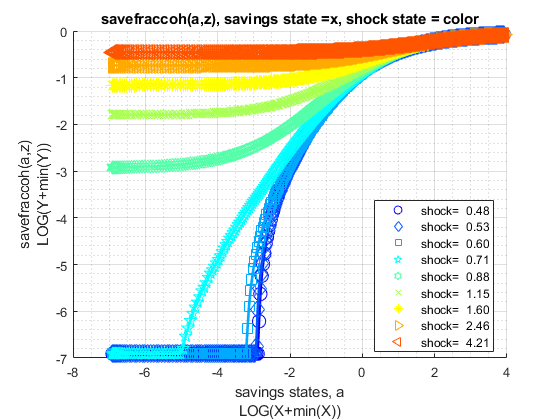
\includegraphics[width=5.20833in,height=\textheight]{img/fx_vfi_az_bisec_vec_images/figure_5.png}

\hypertarget{test-ff_vfi_az_bisec_vec-with-higher-uncertainty}{%
\subsection{Test FF\_VFI\_AZ\_BISEC\_VEC with Higher Uncertainty}\label{test-ff_vfi_az_bisec_vec-with-higher-uncertainty}}

Increase the standard deviation of the Shock.

\begin{verbatim}
mp_support = containers.Map('KeyType','char', 'ValueType','any');
mp_support('bl_print_params') = false;
mp_support('bl_print_iterinfo') = false;
mp_support('ls_ffcmd') = {'savefraccoh'};
mp_support('ls_ffsna') = {};
mp_support('ls_ffgrh') = {};
mp_params = containers.Map('KeyType','char', 'ValueType','any');
mp_params('it_a_n') = 150;
mp_params('it_z_n') = 15;
mp_params('fl_a_max') = 50;
mp_params('st_grid_type') = 'grid_powerspace';
% graph color spectrum
mp_params('cl_colors') = 'copper';
\end{verbatim}

Lower standard deviation of shock:

\begin{verbatim}
% Lower Risk Aversion
mp_params('fl_shk_std') = 0.10;
ff_vfi_az_bisec_vec(mp_params, mp_support);

Elapsed time is 2.595920 seconds.
----------------------------------------
xxxxxxxxxxxxxxxxxxxxxxxxxxxxxxxxxxxxxxxx
CONTAINER NAME: mp_ffcmd ND Array (Matrix etc)
xxxxxxxxxxxxxxxxxxxxxxxxxxxxxxxxxxxxxxxx
                   i    idx    ndim    numel    rowN    colN     sum       mean        std      coefvari    min      max  
                   _    ___    ____    _____    ____    ____    ______    _______    _______    ________    ___    _______

    savefraccoh    1     1      2      2250     150      15     1507.5    0.67001    0.28668    0.42788      0     0.92568

xxx TABLE:savefraccoh xxxxxxxxxxxxxxxxxx
              c1         c2         c3         c4         c5         c11        c12        c13        c14        c15  
            _______    _______    _______    _______    _______    _______    _______    _______    _______    _______

    r1            0          0          0          0          0    0.13847    0.18485    0.23026    0.27378    0.31729
    r2            0          0          0          0          0    0.13853    0.18491    0.23032    0.27384    0.31736
    r3            0          0          0          0          0    0.13895    0.18528    0.23063    0.27408     0.3176
    r4            0          0          0          0          0    0.13987    0.18607     0.2313    0.27469    0.31809
    r5            0          0          0          0          0    0.14011    0.18735     0.2324    0.27567    0.31888
    r146    0.92373    0.92354     0.9233    0.92312    0.92287    0.92086    0.92068    0.92049    0.91952    0.91933
    r147    0.92422    0.92403    0.92385    0.92361    0.92342    0.92141    0.92123    0.92098    0.92007    0.91988
    r148     0.9247    0.92452    0.92434    0.92409    0.92391     0.9219    0.92171    0.92153    0.92062    0.92043
    r149    0.92519    0.92501    0.92483    0.92458     0.9244    0.92245    0.92226    0.92208    0.92116     0.9211
    r150    0.92568     0.9255    0.92531    0.92507    0.92489    0.92293    0.92275    0.92257    0.92245    0.92232
\end{verbatim}

Higher shock standard deviation: low shock high asset save more, high
shock more asset save less, high shock low asset save more:

\begin{verbatim}
% Higher Risk Aversion
mp_params('fl_shk_std') = 0.40;
ff_vfi_az_bisec_vec(mp_params, mp_support);

Elapsed time is 2.805227 seconds.
----------------------------------------
xxxxxxxxxxxxxxxxxxxxxxxxxxxxxxxxxxxxxxxx
CONTAINER NAME: mp_ffcmd ND Array (Matrix etc)
xxxxxxxxxxxxxxxxxxxxxxxxxxxxxxxxxxxxxxxx
                   i    idx    ndim    numel    rowN    colN     sum       mean        std      coefvari    min      max  
                   _    ___    ____    _____    ____    ____    ______    _______    _______    ________    ___    _______

    savefraccoh    1     1      2      2250     150      15     1685.6    0.74914    0.22909     0.3058      0     0.93679

xxx TABLE:savefraccoh xxxxxxxxxxxxxxxxxx
              c1         c2         c3         c4         c5         c11        c12        c13        c14        c15  
            _______    _______    _______    _______    _______    _______    _______    _______    _______    _______

    r1            0          0          0          0          0     0.5264    0.61264    0.68271    0.73922    0.78433
    r2            0          0          0          0          0    0.52646    0.61264    0.68271    0.73922    0.78433
    r3            0          0          0          0          0    0.52658     0.6127    0.68271    0.73922    0.78433
    r4            0          0          0          0          0    0.52682    0.61288    0.68283    0.73928    0.78439
    r5            0          0          0          0          0    0.52731    0.61313    0.68295    0.73934    0.78439
    r146    0.92983    0.92928    0.92873    0.92806    0.92739    0.92269    0.92354     0.9258    0.92904    0.93331
    r147     0.9302    0.92971     0.9291    0.92849    0.92788    0.92361    0.92477     0.9269    0.93001    0.93423
    r148    0.93056    0.93008    0.92953    0.92892    0.92831    0.92458    0.92593      0.928    0.93105    0.93508
    r149    0.93093    0.93044    0.92995    0.92934    0.92873     0.9258    0.92702     0.9291    0.93203      0.936
    r150     0.9313    0.93087    0.93032    0.92977    0.92916    0.92696    0.92818    0.93014    0.93294    0.93679
\end{verbatim}

\hypertarget{ff_vfi_az_mzoom_loop-savings-loop-exact-value-examples}{%
\section{FF\_VFI\_AZ\_MZOOM\_LOOP Savings Loop Exact (VALUE) Examples}\label{ff_vfi_az_mzoom_loop-savings-loop-exact-value-examples}}

\begin{quote}
Go back to \href{http://fanwangecon.github.io/}{fan}'s \href{https://fanwangecon.github.io/MEconTools/}{MEconTools} Toolbox (\href{https://fanwangecon.github.io/MEconTools/bookdown}{bookdown}), \href{https://fanwangecon.github.io/M4Econ/}{Matlab Code Examples} Repository (\href{https://fanwangecon.github.io/M4Econ/bookdown}{bookdown}), or \href{https://fanwangecon.github.io/Math4Econ/}{Math for Econ with Matlab} Repository (\href{https://fanwangecon.github.io/Math4Econ/bookdown}{bookdown}).
\end{quote}

This is the example vignette for function:\href{https://github.com/FanWangEcon/MEconTools/blob/master/MEconTools/vfi/ff_vfi_az_mzoom_loop.m}{\textbf{ff\_vfi\_az\_mzoom\_loop}}
from the \href{https://fanwangecon.github.io/MEconTools/}{\textbf{MEconTools
Package}}\textbf{.} This function
solves the dynamic programming problem for a (a,z) model. The
state-space is on a grid, but choice grids are in terms of \textbf{percentage
of resources} to save and solved exactly.

This is a \textbf{looped} code for \textbf{continuous} choices, solved with the
\href{https://fanwangecon.github.io/MEconTools/MEconTools/doc/optim/htmlpdfm/fx_optim_mzoom_savezrone.html}{\textbf{mzoom}}
algorithm. In contrast to the
\href{https://fanwangecon.github.io/MEconTools/MEconTools/doc/optim/htmlpdfm/fx_optim_bisec_savezrone.html}{\textbf{bisection}}
based solution, this is slower, but this does not rely on first order
conditions.

\textbf{Links to Other Code:}

Core Savings/Borrowing Dynamic Programming Solution Functions that are
functions in the \href{https://fanwangecon.github.io/MEconTools/}{\textbf{MEconTools
Package}}\textbf{.} :

\begin{itemize}
\item
  Common Choice and States Grid :
  \href{https://github.com/FanWangEcon/MEconTools/blob/master/MEconTools/vfi/ff_vfi_az_loop.m}{\textbf{ff\_vfi\_az\_loop}}
\item
  Common Choice and States Grid :
  \href{https://github.com/FanWangEcon/MEconTools/blob/master/MEconTools/vfi/ff_vfi_az_vec.m}{\textbf{ff\_vfi\_az\_vec}}
\item
  States Grid + Continuous Exact Savings as Share of Cash-on-Hand,
  rely on FOC, :\href{https://github.com/FanWangEcon/MEconTools/blob/master/MEconTools/vfi/ff_vfi_az_bisec_loop.m}{\textbf{ff\_vfi\_az\_bisec\_loop}}
\item
  States Grid + Continuous Exact Savings as Share of Cash-on-Hand,
  rely on FOC :
  \href{https://github.com/FanWangEcon/MEconTools/blob/master/MEconTools/vfi/ff_vfi_az_bisec_vec.m}{\textbf{ff\_vfi\_az\_bisec\_vec}}
\item
  States Grid + Continuous Exact Savings as Share of Cash-on-Hand,
  VALUE comparison, :\href{https://github.com/FanWangEcon/MEconTools/blob/master/MEconTools/vfi/ff_vfi_az_mzoom_loop.m}{\textbf{ff\_vfi\_az\_mzoom\_loop}}
\item
  States Grid + Continuous Exact Savings as Share of Cash-on-Hand,
  VALUE comparison, :
  \href{https://github.com/FanWangEcon/MEconTools/blob/master/MEconTools/vfi/ff_vfi_az_mzoom_vec.m}{\textbf{ff\_vfi\_az\_mzoom\_vec}}
\end{itemize}

\hypertarget{test-ff_vfi_az_mzoom_loop-defaults}{%
\subsection{Test FF\_VFI\_AZ\_MZOOM\_LOOP Defaults}\label{test-ff_vfi_az_mzoom_loop-defaults}}

Call the function with defaults. By default, shows the asset policy
function summary. Model parameters can be changed by the mp\_params.

\begin{verbatim}
%mp_params
mp_params = containers.Map('KeyType','char', 'ValueType','any');
mp_params('fl_crra') = 1.5;
mp_params('fl_beta') = 0.94;
% call function
ff_vfi_az_mzoom_loop(mp_params);

Elapsed time is 83.956071 seconds.
----------------------------------------
xxxxxxxxxxxxxxxxxxxxxxxxxxxxxxxxxxxxxxxx
CONTAINER NAME: mp_ffcmd ND Array (Matrix etc)
xxxxxxxxxxxxxxxxxxxxxxxxxxxxxxxxxxxxxxxx
          i    idx    ndim    numel    rowN    colN     sum       mean      std      coefvari    min     max  
          _    ___    ____    _____    ____    ____    ______    ______    ______    ________    ___    ______

    ap    1     1      2       700     100      7      9861.5    14.088    14.386     1.0212      0     50.115

xxx TABLE:ap xxxxxxxxxxxxxxxxxx
              c1        c2        c3         c4         c5         c6         c7  
            ______    ______    ______    ________    _______    _______    ______

    r1           0         0         0     0.05343    0.25568    0.60598    1.1155
    r2           0         0         0    0.053451    0.25571    0.60652    1.1161
    r3           0         0         0    0.056468    0.25574    0.60897    1.1174
    r4           0         0         0    0.061232    0.25995    0.61042    1.1238
    r5           0         0         0    0.065929     0.2689    0.61091    1.1323
    r96     43.387    43.517      43.7      43.922     44.221     44.657    45.225
    r97     44.562    44.694    44.876      45.095     45.392     45.847    46.394
    r98     45.758     45.89    46.071      46.287     46.583     47.037    47.596
    r99     46.972    47.103    47.285        47.5     47.794     48.247    48.812
    r100    48.183    48.337    48.518      48.732     49.025     49.478    50.115
\end{verbatim}

\hypertarget{test-ff_vfi_az_mzoom_loop-speed-tests}{%
\subsection{Test FF\_VFI\_AZ\_MZOOM\_LOOP Speed Tests}\label{test-ff_vfi_az_mzoom_loop-speed-tests}}

Call the function with defaults. By default, shows the asset policy
function summary. Model parameters can be changed by the mp\_params.

\begin{verbatim}
mp_support = containers.Map('KeyType','char', 'ValueType','any');
mp_support('bl_timer') = true;
mp_support('ls_ffcmd') = {};
\end{verbatim}

A grid 50, shock grid 5:

\begin{verbatim}
mp_params = containers.Map('KeyType','char', 'ValueType','any');
mp_params('it_a_n') = 50;
mp_params('it_z_n') = 5;
ff_vfi_az_mzoom_loop(mp_params, mp_support);

Elapsed time is 26.554641 seconds.
\end{verbatim}

A grid 750, shock grid 15:

\begin{verbatim}
mp_params = containers.Map('KeyType','char', 'ValueType','any');
mp_params('it_a_n') = 750;
mp_params('it_z_n') = 15;
ff_vfi_az_mzoom_loop(mp_params, mp_support);

Elapsed time is 2148.508425 seconds.
\end{verbatim}

A grid 600, shock grid 45:

\begin{verbatim}
mp_params = containers.Map('KeyType','char', 'ValueType','any');
mp_params('it_a_n') = 600;
mp_params('it_z_n') = 45;
ff_vfi_az_mzoom_loop(mp_params, mp_support);

Elapsed time is 8507.097739 seconds.
\end{verbatim}

\hypertarget{test-ff_vfi_az_mzoom_loop-control-outputs}{%
\subsection{Test FF\_VFI\_AZ\_MZOOM\_LOOP Control Outputs}\label{test-ff_vfi_az_mzoom_loop-control-outputs}}

Run the function first without any outputs, but only the timer.

\begin{verbatim}
mp_params = containers.Map('KeyType','char', 'ValueType','any');
mp_params('it_a_n') = 50;
mp_params('it_z_n') = 5;
mp_support = containers.Map('KeyType','char', 'ValueType','any');
mp_support('bl_timer') = true;
mp_support('bl_print_params') = false;
mp_support('bl_print_iterinfo') = false;
mp_support('ls_ffcmd') = {};
ff_vfi_az_mzoom_loop(mp_params, mp_support);

Elapsed time is 24.011245 seconds.
\end{verbatim}

Run the function and show policy function for savings choice. For
ls\_ffcmd, ls\_ffsna, ls\_ffgrh, can include these: `v', `ap', `c', `y',
`coh', `savefraccoh'. These are value, aprime savings choice,
consumption, income, cash on hand, and savings fraction as cash-on-hand.

\begin{verbatim}
mp_support = containers.Map('KeyType','char', 'ValueType','any');
mp_support('bl_print_params') = false;
mp_support('bl_print_iterinfo') = false;
% ls_ffcmd: summary print which outcomes
mp_support('ls_ffcmd') = {};
% ls_ffsna: detail print which outcomes
mp_support('ls_ffsna') = {'savefraccoh'};
% ls_ffgrh: graphical print which outcomes
mp_support('ls_ffgrh') = {'savefraccoh'};
ff_vfi_az_mzoom_loop(mp_params, mp_support);

Elapsed time is 23.773078 seconds.
xxx  ff_vfi_az_vec, outcome=savefraccoh  xxxxxxxxxxxxxxxxxxxxxxxxxxx
    group       a        mean_z_0_4858    mean_z_0_67798    mean_z_0_9462    mean_z_1_3205    mean_z_1_8429
    _____    ________    _____________    ______________    _____________    _____________    _____________

      1             0             0                 0         0.067148           0.2084          0.35952   
      2      0.002975             0                 0         0.069345          0.20826          0.36029   
      3      0.016829             0                 0         0.070749           0.2136          0.36206   
      4      0.046375             0         0.0059631          0.08732          0.22641          0.36263   
      5      0.095198      0.008725          0.033935          0.11637          0.24674           0.3747   
      6        0.1663      0.054327          0.077152          0.15198          0.26635          0.39127   
      7       0.26234      0.099882           0.13131           0.1936          0.29922          0.41248   
      8       0.38568       0.15954            0.1928          0.24107          0.33005          0.43049   
      9       0.53852       0.23411           0.25482          0.29164          0.37407           0.4593   
     10       0.72291       0.30704           0.31604          0.34806          0.41148          0.48371   
     11       0.94076       0.37567           0.37487          0.40768          0.44925          0.50972   
     12        1.1939       0.43849           0.42939           0.4573          0.48691          0.54333   
     13         1.484       0.49491           0.48129          0.50332          0.53253          0.56934   
     14        1.8128       0.54486           0.53013          0.54642          0.56773          0.59615   
     15        2.1817       0.58868           0.57335          0.58545          0.60016          0.62817   
     16        2.5924        0.6271           0.61254          0.62056          0.63057          0.65247   
     17        3.0463       0.66058            0.6468          0.65237          0.65884          0.67518   
     18        3.5449       0.69019           0.67699          0.68069          0.68379          0.69636   
     19        4.0894       0.71615           0.70375           0.7058          0.70719           0.7159   
     20        4.6813       0.73661           0.72701          0.72843          0.72781          0.73341   
     21        5.3218       0.75302            0.7481          0.74821          0.74661          0.74981   
     22        6.0121       0.76912           0.76622          0.76622          0.76342          0.76534   
     23        6.7536       0.78503           0.78285          0.78223          0.77885          0.78383   
     24        7.5474       0.79943           0.79703          0.79623          0.79223          0.79677   
     25        8.3948       0.81264           0.81024           0.8093          0.80504          0.80784   
     26        9.2967       0.82384           0.82198          0.82064          0.81634          0.81874   
     27        10.254       0.83447           0.83225          0.83065          0.82653          0.82824   
     28        11.269       0.84345           0.84174          0.84025          0.83545          0.83703   
     29        12.342       0.85185           0.85017          0.84865          0.84417          0.84497   
     30        13.473       0.85962           0.85746          0.85642          0.85178          0.85185   
     31        14.665       0.86626           0.86466          0.86306          0.85873          0.85895   
     32        15.918       0.87226           0.87066          0.86959          0.86504          0.86466   
     33        17.233       0.87786           0.87626          0.87529          0.87146          0.87061   
     34        18.611       0.88332           0.88182          0.88026          0.87766          0.87546   
     35        20.053         0.888           0.88656          0.88507          0.88267          0.88026   
     36         21.56       0.89187           0.89087          0.88947          0.88825          0.88483   
     37        23.133       0.89587           0.89484          0.89347          0.89256          0.88867   
     38        24.773        0.8997           0.89827          0.89727          0.89587          0.89259   
     39        26.481         0.903           0.90147          0.90066          0.89964          0.89587   
     40        28.258       0.90601           0.90467          0.90376          0.90278          0.89907   
     41        30.104       0.90881            0.9077          0.90628          0.90547          0.90216   
     42        32.021       0.91137           0.91035          0.90908          0.90838          0.90467   
     43         34.01       0.91377           0.91275          0.91148          0.91068          0.90708   
     44         36.07       0.91595           0.91468          0.91388          0.91308          0.90983   
     45        38.204       0.91788           0.91708          0.91617          0.91531          0.91204   
     46        40.412       0.91948           0.91868          0.91788          0.91708          0.91388   
     47        42.695       0.92168           0.92085          0.91998          0.91915          0.91604   
     48        45.053       0.92331           0.92251          0.92171          0.92091          0.91788   
     49        47.488       0.92485           0.92408          0.92331          0.92254           0.9202   
     50            50       0.92588           0.92555          0.92485          0.92423          0.92402   
\end{verbatim}

\includegraphics[width=5.20833in,height=\textheight]{img/fx_vfi_az_mzoom_loop_images/figure_0.png}

\includegraphics[width=5.20833in,height=\textheight]{img/fx_vfi_az_mzoom_loop_images/figure_1.png}

Run the function and show summaries for savings and fraction of coh
saved:

\begin{verbatim}
%mp_params
mp_params = containers.Map('KeyType','char', 'ValueType','any');
% mp_params('fl_crra') = 1.5;
% mp_params('fl_beta') = 0.94;
mp_params('it_a_n') = 100;
mp_params('it_z_n') = 9;
mp_support = containers.Map('KeyType','char', 'ValueType','any');
mp_support('bl_print_params') = false;
mp_support('bl_print_iterinfo') = false;
% ls_ffcmd: summary print which outcomes
mp_support('ls_ffcmd') = {};
% ls_ffsna: detail print which outcomes
mp_support('ls_ffsna') = {'savefraccoh'};
% ls_ffgrh: graphical print which outcomes
mp_support('ls_ffgrh') = {'savefraccoh'};
% call function
ff_vfi_az_mzoom_loop(mp_params, mp_support);

Elapsed time is 111.419370 seconds.
xxx  ff_vfi_az_vec, outcome=savefraccoh  xxxxxxxxxxxxxxxxxxxxxxxxxxx
    group        a         mean_z_0_36853    mean_z_0_46648    mean_z_0_59047    mean_z_0_74742    mean_z_0_94608    mean_z_1_1975    mean_z_1_5159    mean_z_1_9188    mean_z_2_4288
    _____    __________    ______________    ______________    ______________    ______________    ______________    _____________    _____________    _____________    _____________

       1              0               0                0                 0                  0         0.065547          0.16519          0.27438          0.37327          0.46242   
       2     0.00051272               0                0                 0                  0         0.066347          0.16588          0.27443           0.3738           0.4625   
       3      0.0029004               0                0                 0                  0         0.067948          0.16679          0.27523          0.37407           0.4625   
       4      0.0079925               0                0                 0         0.00050216         0.069549          0.16975          0.27721          0.37559           0.4633   
       5       0.016407               0                0                 0           0.005563         0.071534          0.17359           0.2802          0.37727           0.4649   
       6       0.028662               0                0                 0           0.011926         0.080274          0.17999          0.28363          0.38054           0.4665   
       7       0.045213               0                0                 0           0.022095         0.090757          0.18443          0.28523          0.38087           0.4665   
       8        0.06647               0                0         0.0043625           0.033935          0.10076          0.19478          0.29244          0.38621           0.4697   
       9       0.092813      0.00076108        0.0091251          0.017748           0.047979          0.11397           0.2068          0.30084          0.39207          0.47371   
      10        0.12459         0.02539         0.027791          0.036336           0.066347          0.13237          0.21681          0.31124          0.39938          0.47898   
      11        0.16214        0.049062         0.054743          0.057497           0.087289          0.14878          0.23341          0.31965           0.4076          0.48451   
      12        0.20576        0.080353         0.076351          0.084213            0.11115          0.16729          0.24668          0.33295          0.41295          0.48895   
      13        0.25576         0.11036          0.10076           0.11357            0.13677           0.1944          0.26643          0.34326          0.42327          0.49539   
      14        0.31242         0.14798          0.12866           0.14076            0.16483          0.21731          0.28363          0.35886          0.43195          0.50332   
      15        0.37601         0.17839          0.16439           0.16895              0.194          0.24107          0.30164          0.37165          0.44362          0.51204   
      16         0.4468          0.2098          0.20032            0.1988            0.22401          0.26563          0.32575          0.38953           0.4565          0.51772   
      17        0.52503         0.24246          0.23721           0.23371            0.25482          0.29153          0.34564          0.40412          0.46694          0.52773   
      18        0.61095         0.28123          0.27422           0.26803            0.28577          0.31725          0.36526          0.42169          0.48129           0.5355   
      19         0.7048         0.31861          0.30964           0.30224            0.31644          0.34326          0.38636          0.43889          0.49228          0.54649   
      20         0.8068         0.35352          0.34406           0.33561            0.34646          0.37247          0.41168           0.4555          0.50395          0.55454   
      21        0.91719         0.38727          0.37774           0.36766            0.37639          0.40048          0.43289          0.47181          0.51932          0.56671   
      22         1.0362         0.42001          0.40688           0.39888            0.40495          0.42569           0.4541          0.49222          0.53173          0.57495   
      23          1.164          0.4501          0.43289           0.42881            0.43266           0.4501          0.47451          0.50812          0.54573          0.58735   
      24         1.3008         0.47851          0.45746           0.45719            0.45922          0.47371           0.4948          0.52453           0.5608          0.59678   
      25         1.4468         0.50572          0.48514           0.48371            0.48451          0.49652          0.51432          0.54067          0.57335          0.60616   
      26         1.6023         0.53093          0.51118           0.50952            0.50892          0.51852          0.53322          0.56014          0.58575          0.61895   
      27         1.7673         0.55214          0.53571           0.53333            0.53173          0.53973          0.55258          0.57573          0.60152          0.62867   
      28         1.9422         0.57052          0.55854           0.55614            0.55374          0.55981          0.57335          0.59055          0.61336          0.63834   
      29          2.127         0.58782          0.58031           0.57735            0.57415          0.57893          0.59055          0.60534          0.62569          0.65071   
      30         2.3221         0.60768          0.60016           0.59758            0.59375          0.59695          0.60696           0.6194           0.6375          0.65978   
      31         2.5275         0.62577          0.61947           0.61496            0.61226          0.61416          0.62256          0.63297          0.65018          0.66898   
      32         2.7434         0.64351          0.63697           0.63101            0.62956          0.63057           0.6376          0.64617          0.66298          0.68097   
      33           2.97         0.65976          0.65338           0.64537            0.64591          0.64617          0.65178          0.66218          0.67378          0.68986   
      34         3.2075         0.67458          0.66898           0.66058            0.66124          0.66058          0.66498          0.67432          0.68445          0.69819   
      35          3.456         0.68919          0.68379           0.67538            0.67538          0.67458          0.67829          0.68592          0.69419          0.70716   
      36         3.7158          0.7022          0.69739           0.68939            0.68928          0.68779          0.69019          0.69659           0.7042           0.7154   
      37         3.9869          0.7146           0.7098            0.7022            0.70205          0.70039           0.7022           0.7074          0.71372          0.72609   
      38         4.2696         0.72668           0.7218            0.7146             0.7138          0.71209            0.713          0.71779           0.7254          0.73341   
      39          4.564         0.73741          0.73341            0.7262             0.7254          0.72317           0.7234          0.72748          0.73419          0.74121   
      40         4.8702         0.74798          0.74381           0.73711            0.73581          0.73341          0.73341          0.73661          0.74221          0.74821   
      41         5.1884         0.75768          0.75382           0.74727            0.74581          0.74348          0.74301          0.74551          0.75041          0.75542   
      42         5.5188         0.76679           0.7618           0.75684            0.75542          0.75281          0.75217          0.75382          0.75782          0.76232   
      43         5.8615         0.77502          0.76862           0.76542            0.76422          0.76165          0.76022          0.76182          0.76502          0.77102   
      44         6.2166         0.78303          0.77658           0.77422            0.77262          0.76996          0.76862          0.76941          0.77229          0.77742   
      45         6.5844         0.79063          0.78452           0.78223            0.78063          0.77742          0.77633          0.77661          0.77895           0.7835   
      46         6.9649         0.79783          0.79196           0.78983            0.78823          0.78529          0.78356          0.78543          0.78503          0.78903   
      47         7.3583         0.80499          0.79863           0.79695            0.79543          0.79223          0.79043          0.79223          0.79143          0.79463   
      48         7.7647         0.81024          0.80566           0.80343            0.80231          0.79863          0.79699          0.79863          0.79943          0.80023   
      49         8.1844         0.81504          0.81184           0.81003            0.80862          0.80504          0.80329          0.80471          0.80504          0.80547   
      50         8.6173         0.81984          0.81744           0.81584            0.81424          0.81104          0.80997          0.81024          0.81024          0.81024   
      51         9.0637         0.82544          0.82351           0.82144            0.82031          0.81664          0.81584          0.81573          0.81579          0.81733   
      52         9.5237         0.83065          0.82881           0.82664            0.82544          0.82224          0.82224          0.82064          0.82064          0.82191   
      53         9.9975         0.83545          0.83385           0.83217            0.83065          0.82744          0.82704          0.82544          0.82537          0.82624   
      54         10.485         0.84025          0.83863           0.83697            0.83545          0.83225           0.8321          0.83044          0.82985          0.83054   
      55         10.987         0.84494          0.84315           0.84155            0.84023          0.83703          0.83625          0.83465          0.83385          0.83457   
      56         11.502         0.84919          0.84705           0.84585            0.84425          0.84105            0.841          0.83915          0.83785          0.83844   
      57         12.032         0.85319          0.85156           0.85002            0.84785          0.84562          0.84505          0.84322          0.84185          0.84185   
      58         12.577         0.85666          0.85506           0.85396            0.85174          0.84945          0.84865          0.84665          0.84585          0.84574   
      59         13.136         0.86064          0.85906           0.85746            0.85506          0.85338          0.85265          0.85079          0.84945          0.84919   
      60         13.709         0.86386          0.86226           0.86122            0.85826          0.85666          0.85639          0.85425          0.85265          0.85245   
      61         14.298         0.86706          0.86596           0.86461            0.86138          0.86042          0.85978          0.85746          0.85586          0.85562   
      62         14.901         0.87052          0.86906           0.86746            0.86464          0.86372          0.86304          0.86066          0.85906          0.85826   
      63         15.519         0.87306          0.87215           0.87066            0.86746          0.86682          0.86615          0.86386          0.86226          0.86146   
      64         16.152         0.87626          0.87466           0.87378            0.87066          0.86981          0.86906          0.86698          0.86535          0.86464   
      65         16.801         0.87866          0.87779           0.87626             0.8736          0.87226          0.87196          0.86981          0.86812           0.8687   
      66         17.465         0.88163          0.88026           0.87923            0.87626          0.87538          0.87466          0.87226          0.87066          0.87126   
      67         18.144         0.88409          0.88267           0.88179            0.87866          0.87786          0.87706          0.87466          0.87386          0.87375   
      68         18.839         0.88646          0.88507           0.88422            0.88107          0.88026          0.87946           0.8776          0.87706          0.87612   
      69          19.55         0.88867          0.88747           0.88653            0.88347          0.88267          0.88187          0.87997          0.87946          0.87843   
      70         20.277         0.89087          0.88947           0.88867            0.88587          0.88507          0.88427          0.88187          0.88187          0.88026   
      71          21.02         0.89267          0.89187           0.89087            0.88787          0.88736          0.88659          0.88427          0.88419          0.88267   
      72         21.778         0.89493          0.89347           0.89267            0.89027          0.88945          0.88867          0.88656          0.88587          0.88477   
      73         22.553         0.89667          0.89582           0.89487            0.89187          0.89107          0.89027          0.88859          0.88825          0.88667   
      74         23.345         0.89827          0.89747           0.89667            0.89422          0.89336          0.89262          0.89027          0.89016          0.88862   
      75         24.152         0.90034          0.89907           0.89827            0.89587          0.89507          0.89427          0.89237          0.89187          0.89027   
      76         24.977         0.90204          0.90111           0.89987            0.89747          0.89667          0.89587          0.89416          0.89347          0.89187   
      77         25.818         0.90361          0.90274           0.90147            0.89907          0.89827          0.89797          0.89587          0.89507          0.89347   
      78         26.675         0.90515          0.90387           0.90307            0.90067          0.89987          0.89961          0.89747          0.89711          0.89551   
      79          27.55         0.90628          0.90547           0.90467            0.90227          0.90147          0.90117          0.89907          0.89827          0.89667   
      80         28.441         0.90788          0.90708           0.90547            0.90387          0.90307          0.90227          0.90066          0.89987          0.89827   
      81          29.35         0.90908           0.9086           0.90708            0.90547          0.90467          0.90387          0.90213          0.90147          0.89987   
      82         30.276         0.91068          0.90988           0.90825            0.90697          0.90623          0.90547          0.90354          0.90307          0.90146   
      83         31.219         0.91195          0.91121           0.90908            0.90828          0.90758           0.9069          0.90467          0.90444          0.90281   
      84         32.179         0.91308          0.91228           0.91035            0.90958          0.90887          0.90788          0.90623          0.90547          0.90387   
      85         33.157         0.91388          0.91361           0.91148            0.91068          0.90988          0.90908          0.90708          0.90703           0.9054   
      86         34.153         0.91543          0.91468           0.91228            0.91198           0.9113          0.91063          0.90872          0.90788          0.90628   
      87         35.166         0.91628          0.91548            0.9138            0.91308          0.91228          0.91148          0.90988          0.90908           0.9078   
      88         36.198         0.91708          0.91688           0.91468            0.91388          0.91355          0.91291          0.91068          0.91057          0.90893   
      89         37.247         0.91851          0.91786           0.91548            0.91527          0.91463          0.91388          0.91214          0.91148          0.90988   
      90         38.314         0.91946          0.91868           0.91691            0.91628          0.91548          0.91468          0.91308          0.91228          0.91108   
      91         39.399         0.92028          0.91948           0.91788            0.91708          0.91628          0.91604          0.91422          0.91374          0.91228   
      92         40.503         0.92108          0.92028           0.91868            0.91788          0.91761            0.917           0.9154          0.91468          0.91388   
      93         41.625         0.92188          0.92108           0.91948            0.91868          0.91851          0.91788          0.91628          0.91548          0.91527   
      94         42.765         0.92268          0.92188           0.92028            0.92001           0.9194          0.91868          0.91771          0.91628           0.9162   
      95         43.924         0.92348          0.92268           0.92108            0.92085          0.92026          0.91948          0.91868          0.91708          0.91708   
      96         45.102         0.92428          0.92348           0.92188            0.92168          0.92108          0.92028          0.91948          0.91838          0.91788   
      97         46.298         0.92508          0.92414           0.92268            0.92248          0.92188          0.92108          0.92028          0.91931          0.91868   
      98         47.513         0.92588          0.92469           0.92348            0.92325          0.92268          0.92188          0.92168          0.92026          0.92028   
      99         48.747         0.92668          0.92508           0.92428            0.92398          0.92347          0.92268          0.92248          0.92108           0.9218   
     100             50         0.92737           0.9258           0.92508            0.92428           0.9242          0.92348          0.92337          0.92334          0.92348   
\end{verbatim}

\includegraphics[width=5.20833in,height=\textheight]{img/fx_vfi_az_mzoom_loop_images/figure_2.png}

\includegraphics[width=5.20833in,height=\textheight]{img/fx_vfi_az_mzoom_loop_images/figure_3.png}

\hypertarget{test-ff_vfi_az_mzoom_loop-change-interest-rate-and-discount}{%
\subsection{Test FF\_VFI\_AZ\_MZOOM\_LOOP Change Interest Rate and Discount}\label{test-ff_vfi_az_mzoom_loop-change-interest-rate-and-discount}}

Show only save fraction of cash on hand:

\begin{verbatim}
mp_support = containers.Map('KeyType','char', 'ValueType','any');
mp_support('bl_print_params') = false;
mp_support('bl_print_iterinfo') = false;
mp_support('ls_ffcmd') = {'savefraccoh'};
mp_support('ls_ffsna') = {};
mp_support('ls_ffgrh') = {};
mp_params = containers.Map('KeyType','char', 'ValueType','any');
mp_params('it_a_n') = 750;
mp_params('it_z_n') = 9;
mp_params('fl_a_max') = 50;
mp_params('st_grid_type') = 'grid_powerspace';
\end{verbatim}

Solve the model with several different interest rates and discount
factor:

\begin{verbatim}
% Lower Savings Incentives
mp_params('fl_beta') = 0.80;
mp_params('fl_r') = 0.01;
ff_vfi_az_mzoom_loop(mp_params, mp_support);

Elapsed time is 294.329574 seconds.
----------------------------------------
xxxxxxxxxxxxxxxxxxxxxxxxxxxxxxxxxxxxxxxx
CONTAINER NAME: mp_ffcmd ND Array (Matrix etc)
xxxxxxxxxxxxxxxxxxxxxxxxxxxxxxxxxxxxxxxx
                   i    idx    ndim    numel    rowN    colN     sum       mean       std      coefvari    min      max  
                   _    ___    ____    _____    ____    ____    ______    ______    _______    ________    ___    _______

    savefraccoh    1     1      2      6750     750      9      3468.2    0.5138    0.27192    0.52924      0     0.80103

xxx TABLE:savefraccoh xxxxxxxxxxxxxxxxxx
              c1         c2         c3         c4         c5         c6         c7         c8          c9   
            _______    _______    _______    _______    _______    _______    _______    _______    ________

    r1            0          0          0          0          0          0          0    0.02073    0.065955
    r2            0          0          0          0          0          0          0    0.02073    0.065955
    r3            0          0          0          0          0          0          0    0.02073    0.065955
    r4            0          0          0          0          0          0          0    0.02073    0.065955
    r5            0          0          0          0          0          0          0    0.02073    0.065987
    r746     0.8008    0.79843     0.7959    0.79303    0.78983    0.78663    0.78303    0.77903     0.77502
    r747    0.80092    0.79855    0.79603    0.79303    0.79058    0.78713    0.78362    0.77953     0.77553
    r748    0.80102    0.79863    0.79615     0.7935    0.79063    0.78729    0.78378    0.77972     0.77568
    r749    0.80103    0.79863    0.79623    0.79369    0.79063    0.78743    0.78383    0.77983     0.77582
    r750    0.80103    0.79904    0.79623    0.79378    0.79063    0.78743    0.78383    0.77983     0.77582

% Higher Savings Incentives
mp_params('fl_beta') = 0.95;
mp_params('fl_r') = 0.04;
ff_vfi_az_mzoom_loop(mp_params, mp_support);

Elapsed time is 1309.412430 seconds.
----------------------------------------
xxxxxxxxxxxxxxxxxxxxxxxxxxxxxxxxxxxxxxxx
CONTAINER NAME: mp_ffcmd ND Array (Matrix etc)
xxxxxxxxxxxxxxxxxxxxxxxxxxxxxxxxxxxxxxxx
                   i    idx    ndim    numel    rowN    colN     sum       mean       std      coefvari    min      max  
                   _    ___    ____    _____    ____    ____    ______    ______    _______    ________    ___    _______

    savefraccoh    1     1      2      6750     750      9      4667.7    0.6915    0.26685     0.3859      0     0.92668

xxx TABLE:savefraccoh xxxxxxxxxxxxxxxxxx
              c1         c2         c3         c4          c5         c6         c7         c8         c9   
            _______    _______    _______    _______    ________    _______    _______    _______    _______

    r1            0          0          0          0      0.0647    0.16668    0.27352    0.37327     0.4617
    r2            0          0          0          0      0.0647    0.16668    0.27352    0.37327     0.4617
    r3            0          0          0          0    0.064731    0.16668    0.27352    0.37327     0.4617
    r4            0          0          0          0    0.064731    0.16668    0.27355    0.37327     0.4617
    r5            0          0          0          0    0.064747    0.16671    0.27355    0.37327     0.4617
    r746    0.92657    0.92588    0.92508    0.92428     0.92348    0.92268    0.92235    0.92188    0.92188
    r747    0.92664    0.92588    0.92508    0.92428     0.92402    0.92318    0.92248    0.92188    0.92235
    r748    0.92668    0.92588    0.92508    0.92478     0.92411    0.92328     0.9226    0.92188     0.9226
    r749    0.92668    0.92588    0.92555    0.92488      0.9242     0.9234    0.92268    0.92254    0.92268
    r750    0.92668    0.92588    0.92565    0.92497     0.92427    0.92348    0.92268    0.92268    0.92268
\end{verbatim}

\hypertarget{test-ff_vfi_az_mzoom_loop-changing-risk-aversion}{%
\subsection{Test FF\_VFI\_AZ\_MZOOM\_LOOP Changing Risk Aversion}\label{test-ff_vfi_az_mzoom_loop-changing-risk-aversion}}

Here, again, show fraction of coh saved in summary tabular form, but
also show it graphically.

\begin{verbatim}
mp_support = containers.Map('KeyType','char', 'ValueType','any');
mp_support('bl_print_params') = false;
mp_support('bl_print_iterinfo') = false;
mp_support('ls_ffcmd') = {'savefraccoh'};
mp_support('ls_ffsna') = {};
mp_support('ls_ffgrh') = {'savefraccoh'};
mp_params = containers.Map('KeyType','char', 'ValueType','any');
mp_params('it_a_n') = 100;
mp_params('it_z_n') = 7;
mp_params('fl_a_max') = 50;
mp_params('st_grid_type') = 'grid_powerspace';
\end{verbatim}

Solve the model with different risk aversion levels, higher preferences
for risk:

\begin{verbatim}
% Lower Risk Aversion
mp_params('fl_crra') = 0.5;
ff_vfi_az_mzoom_loop(mp_params, mp_support);

Elapsed time is 84.461743 seconds.
----------------------------------------
xxxxxxxxxxxxxxxxxxxxxxxxxxxxxxxxxxxxxxxx
CONTAINER NAME: mp_ffcmd ND Array (Matrix etc)
xxxxxxxxxxxxxxxxxxxxxxxxxxxxxxxxxxxxxxxx
                   i    idx    ndim    numel    rowN    colN     sum       mean        std      coefvari    min      max  
                   _    ___    ____    _____    ____    ____    ______    _______    _______    ________    ___    _______

    savefraccoh    1     1      2       700     100      7      452.03    0.64575    0.28029    0.43406      0     0.90354

xxx TABLE:savefraccoh xxxxxxxxxxxxxxxxxx
              c1         c2         c3          c4           c5         c6         c7   
            _______    _______    _______    _________    ________    _______    _______

    r1            0          0          0    0.0047077    0.089109      0.198    0.30781
    r2            0          0          0    0.0051079    0.089156      0.198    0.30793
    r3            0          0          0    0.0059631    0.090679     0.1988    0.30848
    r4            0          0          0    0.0079639    0.092358    0.20109    0.30964
    r5            0          0          0     0.011926    0.092758    0.20413    0.31171
    r96     0.90047    0.89907    0.89826      0.89727     0.89587    0.89347    0.89267
    r97     0.90127    0.89987    0.89907      0.89822     0.89727    0.89477    0.89394
    r98     0.90204    0.90067    0.89987      0.89907     0.89822    0.89573    0.89493
    r99     0.90278    0.90147    0.90067      0.89987     0.89907    0.89667    0.89587
    r100    0.90354    0.90227    0.90147      0.90067     0.89987    0.89801    0.89667
\end{verbatim}

\includegraphics[width=5.20833in,height=\textheight]{img/fx_vfi_az_mzoom_loop_images/figure_4.png}

\includegraphics[width=5.20833in,height=\textheight]{img/fx_vfi_az_mzoom_loop_images/figure_5.png}

When risk aversion increases, at every state-space point, the household
wants to save more.

\begin{verbatim}
% Higher Risk Aversion
mp_params('fl_crra') = 5;
ff_vfi_az_mzoom_loop(mp_params, mp_support);

Elapsed time is 88.697274 seconds.
----------------------------------------
xxxxxxxxxxxxxxxxxxxxxxxxxxxxxxxxxxxxxxxx
CONTAINER NAME: mp_ffcmd ND Array (Matrix etc)
xxxxxxxxxxxxxxxxxxxxxxxxxxxxxxxxxxxxxxxx
                   i    idx    ndim    numel    rowN    colN     sum     mean       std      coefvari    min      max  
                   _    ___    ____    _____    ____    ____    _____    _____    _______    ________    ___    _______

    savefraccoh    1     1      2       700     100      7      502.6    0.718    0.25437    0.35427      0     0.93587

xxx TABLE:savefraccoh xxxxxxxxxxxxxxxxxx
              c1         c2          c3         c4         c5         c6         c7   
            _______    _______    ________    _______    _______    _______    _______

    r1            0          0     0.04674    0.15532    0.27563    0.39047    0.48771
    r2            0          0    0.047493    0.15525    0.27563    0.39101    0.48771
    r3            0          0    0.049541    0.15685    0.27693    0.39127    0.48834
    r4            0          0    0.054343    0.16018    0.27883    0.39287    0.48923
    r5            0          0    0.062848    0.16566    0.28272    0.39528    0.49071
    r96     0.93269    0.93251     0.93189    0.93108    0.93014    0.92988    0.92968
    r97     0.93349    0.93322     0.93269    0.93189    0.93107    0.93104    0.93108
    r98     0.93429    0.93349     0.93347    0.93269    0.93189    0.93189    0.93269
    r99     0.93507    0.93429     0.93424    0.93349    0.93331    0.93349    0.93429
    r100    0.93575    0.93509     0.93507    0.93488    0.93491    0.93509    0.93587
\end{verbatim}

\includegraphics[width=5.20833in,height=\textheight]{img/fx_vfi_az_mzoom_loop_images/figure_6.png}

\includegraphics[width=5.20833in,height=\textheight]{img/fx_vfi_az_mzoom_loop_images/figure_7.png}

\hypertarget{test-ff_vfi_az_mzoom_loop-with-higher-uncertainty}{%
\subsection{Test FF\_VFI\_AZ\_MZOOM\_LOOP with Higher Uncertainty}\label{test-ff_vfi_az_mzoom_loop-with-higher-uncertainty}}

Increase the standard deviation of the Shock.

\begin{verbatim}
mp_support = containers.Map('KeyType','char', 'ValueType','any');
mp_support('bl_print_params') = false;
mp_support('bl_print_iterinfo') = false;
mp_support('ls_ffcmd') = {'savefraccoh'};
mp_support('ls_ffsna') = {};
mp_support('ls_ffgrh') = {};
mp_params = containers.Map('KeyType','char', 'ValueType','any');
mp_params('it_a_n') = 150;
mp_params('it_z_n') = 15;
mp_params('fl_a_max') = 50;
mp_params('st_grid_type') = 'grid_powerspace';
\end{verbatim}

Lower standard deviation of shock:

\begin{verbatim}
% Lower Risk Aversion
mp_params('fl_shk_std') = 0.10;
ff_vfi_az_mzoom_loop(mp_params, mp_support);

Elapsed time is 304.022067 seconds.
----------------------------------------
xxxxxxxxxxxxxxxxxxxxxxxxxxxxxxxxxxxxxxxx
CONTAINER NAME: mp_ffcmd ND Array (Matrix etc)
xxxxxxxxxxxxxxxxxxxxxxxxxxxxxxxxxxxxxxxx
                   i    idx    ndim    numel    rowN    colN     sum       mean        std      coefvari    min      max  
                   _    ___    ____    _____    ____    ____    ______    _______    _______    ________    ___    _______

    savefraccoh    1     1      2      2250     150      15     1507.2    0.66985    0.28667    0.42796      0     0.92565

xxx TABLE:savefraccoh xxxxxxxxxxxxxxxxxx
              c1         c2         c3         c4         c5         c11        c12        c13        c14        c15  
            _______    _______    _______    _______    _______    _______    _______    _______    _______    _______

    r1            0          0          0          0          0    0.13838    0.18479    0.23021    0.27363    0.31725
    r2            0          0          0          0          0    0.13838    0.18479    0.23027    0.27363    0.31725
    r3            0          0          0          0          0    0.13894    0.18526    0.23041    0.27407    0.31725
    r4            0          0          0          0          0    0.13987    0.18606    0.23121    0.27443    0.31805
    r5            0          0          0          0          0    0.13998    0.18719    0.23201    0.27563    0.31885
    r146    0.92348    0.92348    0.92328    0.92268    0.92268    0.92085    0.92028    0.92028    0.91948    0.91931
    r147     0.9242    0.92398    0.92348    0.92348    0.92337    0.92108    0.92108    0.92097    0.92001    0.91948
    r148    0.92428    0.92428    0.92428    0.92408    0.92348    0.92188    0.92171    0.92108    0.92028    0.92028
    r149    0.92508    0.92497    0.92478    0.92428    0.92428    0.92241    0.92188    0.92188    0.92108    0.92107
    r150    0.92565    0.92508    0.92508    0.92507    0.92485    0.92268    0.92268    0.92254    0.92238    0.92188
\end{verbatim}

Higher shock standard deviation: low shock high asset save more, high
shock more asset save less, high shock low asset save more:

\begin{verbatim}
% Higher Risk Aversion
mp_params('fl_shk_std') = 0.40;
ff_vfi_az_mzoom_loop(mp_params, mp_support);

Elapsed time is 304.175092 seconds.
----------------------------------------
xxxxxxxxxxxxxxxxxxxxxxxxxxxxxxxxxxxxxxxx
CONTAINER NAME: mp_ffcmd ND Array (Matrix etc)
xxxxxxxxxxxxxxxxxxxxxxxxxxxxxxxxxxxxxxxx
                   i    idx    ndim    numel    rowN    colN     sum       mean        std      coefvari    min      max  
                   _    ___    ____    _____    ____    ____    ______    _______    _______    ________    ___    _______

    savefraccoh    1     1      2      2250     150      15     1685.2    0.74898    0.22908    0.30585      0     0.93669

xxx TABLE:savefraccoh xxxxxxxxxxxxxxxxxx
              c1         c2         c3         c4         c5         c11        c12        c13        c14        c15  
            _______    _______    _______    _______    _______    _______    _______    _______    _______    _______

    r1            0          0          0          0          0    0.52613    0.61256    0.68259    0.73901    0.78427
    r2            0          0          0          0          0    0.52613    0.61256    0.68259    0.73901     0.7843
    r3            0          0          0          0          0    0.52613    0.61256    0.68259    0.73901     0.7843
    r4            0          0          0          0          0    0.52682    0.61256    0.68259    0.73901    0.78433
    r5            0          0          0          0          0    0.52693    0.61309    0.68259    0.73901    0.78439
    r146    0.92948    0.92925    0.92828    0.92805    0.92737    0.92263    0.92348    0.92577    0.92901    0.93331
    r147    0.93017    0.92948    0.92868    0.92828    0.92748    0.92348    0.92428    0.92668    0.93002    0.93421
    r148    0.93028    0.93005    0.92948    0.92891    0.92827    0.92428    0.92587    0.92799    0.93101    0.93507
    r149    0.93091    0.93028    0.92948    0.92931    0.92828    0.92574    0.92668    0.92904    0.93189    0.93589
    r150    0.93108    0.93082    0.93027    0.92948    0.92868    0.92668    0.92814    0.93008    0.93269    0.93669
\end{verbatim}

\hypertarget{ff_vfi_az_mzoom_vec-savings-vectorized-exact-value-examples}{%
\section{FF\_VFI\_AZ\_MZOOM\_VEC Savings Vectorized Exact (VALUE) Examples}\label{ff_vfi_az_mzoom_vec-savings-vectorized-exact-value-examples}}

\begin{quote}
Go back to \href{http://fanwangecon.github.io/}{fan}'s \href{https://fanwangecon.github.io/MEconTools/}{MEconTools} Toolbox (\href{https://fanwangecon.github.io/MEconTools/bookdown}{bookdown}), \href{https://fanwangecon.github.io/M4Econ/}{Matlab Code Examples} Repository (\href{https://fanwangecon.github.io/M4Econ/bookdown}{bookdown}), or \href{https://fanwangecon.github.io/Math4Econ/}{Math for Econ with Matlab} Repository (\href{https://fanwangecon.github.io/Math4Econ/bookdown}{bookdown}).
\end{quote}

This is the example vignette for function:\href{https://github.com/FanWangEcon/MEconTools/blob/master/MEconTools/vfi/ff_vfi_az_mzoom_vec.m}{\textbf{ff\_vfi\_az\_mzoom\_vec}}
from the \href{https://fanwangecon.github.io/MEconTools/}{\textbf{MEconTools
Package}}\textbf{.} This function
solves the dynamic programming problem for a (a,z) model. The
state-space is on a grid, but choice grids are in terms of percentage of
resources to save and solved exactly.

This is a \textbf{vectorized} code for \textbf{continuous} choices, solved with
the
\href{https://fanwangecon.github.io/MEconTools/MEconTools/doc/optim/htmlpdfm/fx_optim_mzoom_savezrone.html}{\textbf{mzoom}}
algorithm. In contrast to the
\href{https://fanwangecon.github.io/MEconTools/MEconTools/doc/optim/htmlpdfm/fx_optim_bisec_savezrone.html}{\textbf{bisection}}
based solution, this is slower, but this does not rely on first order
conditions.

\textbf{Links to Other Code:}

Core Savings/Borrowing Dynamic Programming Solution Functions that are
functions in the \href{https://fanwangecon.github.io/MEconTools/}{\textbf{MEconTools
Package}}\textbf{.} :

\begin{itemize}
\item
  Common Choice and States Grid :
  \href{https://github.com/FanWangEcon/MEconTools/blob/master/MEconTools/vfi/ff_vfi_az_loop.m}{\textbf{ff\_vfi\_az\_loop}}
\item
  Common Choice and States Grid :
  \href{https://github.com/FanWangEcon/MEconTools/blob/master/MEconTools/vfi/ff_vfi_az_vec.m}{\textbf{ff\_vfi\_az\_vec}}
\item
  States Grid + Continuous Exact Savings as Share of Cash-on-Hand,
  rely on FOC, :\href{https://github.com/FanWangEcon/MEconTools/blob/master/MEconTools/vfi/ff_vfi_az_bisec_loop.m}{\textbf{ff\_vfi\_az\_bisec\_loop}}
\item
  States Grid + Continuous Exact Savings as Share of Cash-on-Hand,
  rely on FOC :
  \href{https://github.com/FanWangEcon/MEconTools/blob/master/MEconTools/vfi/ff_vfi_az_bisec_vec.m}{\textbf{ff\_vfi\_az\_bisec\_vec}}
\item
  States Grid + Continuous Exact Savings as Share of Cash-on-Hand,
  VALUE comparison, :\href{https://github.com/FanWangEcon/MEconTools/blob/master/MEconTools/vfi/ff_vfi_az_mzoom_loop.m}{\textbf{ff\_vfi\_az\_mzoom\_loop}}
\item
  States Grid + Continuous Exact Savings as Share of Cash-on-Hand,
  VALUE comparison, :
  \href{https://github.com/FanWangEcon/MEconTools/blob/master/MEconTools/vfi/ff_vfi_az_mzoom_vec.m}{\textbf{ff\_vfi\_az\_mzoom\_vec}}
\end{itemize}

\hypertarget{test-ff_vfi_az_mzoom_vec-defaults}{%
\subsection{Test FF\_VFI\_AZ\_MZOOM\_VEC Defaults}\label{test-ff_vfi_az_mzoom_vec-defaults}}

Call the function with defaults. By default, shows the asset policy
function summary. Model parameters can be changed by the mp\_params.

\begin{verbatim}
%mp_params
mp_params = containers.Map('KeyType','char', 'ValueType','any');
mp_params('fl_crra') = 1.5;
mp_params('fl_beta') = 0.94;
% call function
ff_vfi_az_mzoom_vec(mp_params);

Elapsed time is 6.126702 seconds.
----------------------------------------
xxxxxxxxxxxxxxxxxxxxxxxxxxxxxxxxxxxxxxxx
CONTAINER NAME: mp_ffcmd ND Array (Matrix etc)
xxxxxxxxxxxxxxxxxxxxxxxxxxxxxxxxxxxxxxxx
          i    idx    ndim    numel    rowN    colN     sum       mean      std      coefvari    min     max  
          _    ___    ____    _____    ____    ____    ______    ______    ______    ________    ___    ______

    ap    1     1      2       700     100      7      9861.5    14.088    14.386     1.0212      0     50.115

xxx TABLE:ap xxxxxxxxxxxxxxxxxx
              c1        c2        c3         c4         c5         c6         c7  
            ______    ______    ______    ________    _______    _______    ______

    r1           0         0         0     0.05343    0.25568    0.60598    1.1155
    r2           0         0         0    0.053451    0.25571    0.60652    1.1161
    r3           0         0         0    0.056468    0.25574    0.60897    1.1174
    r4           0         0         0    0.061232    0.25995    0.61042    1.1238
    r5           0         0         0    0.065929     0.2689    0.61091    1.1323
    r96     43.387    43.517      43.7      43.922     44.221     44.657    45.225
    r97     44.562    44.694    44.876      45.095     45.392     45.847    46.394
    r98     45.758     45.89    46.071      46.287     46.583     47.037    47.596
    r99     46.972    47.103    47.285        47.5     47.794     48.247    48.812
    r100    48.183    48.337    48.518      48.732     49.025     49.478    50.115
\end{verbatim}

\hypertarget{test-ff_vfi_az_mzoom_vec-speed-tests}{%
\subsection{Test FF\_VFI\_AZ\_MZOOM\_VEC Speed Tests}\label{test-ff_vfi_az_mzoom_vec-speed-tests}}

Call the function with defaults. By default, shows the asset policy
function summary. Model parameters can be changed by the mp\_params.

\begin{verbatim}
mp_support = containers.Map('KeyType','char', 'ValueType','any');
mp_support('bl_timer') = true;
mp_support('ls_ffcmd') = {};
% A grid 50, shock grid 5:
mp_params = containers.Map('KeyType','char', 'ValueType','any');
mp_params('it_a_n') = 50;
mp_params('it_z_n') = 5;
ff_vfi_az_mzoom_vec(mp_params, mp_support);

Elapsed time is 1.996365 seconds.

% A grid 750, shock grid 15:
mp_params = containers.Map('KeyType','char', 'ValueType','any');
mp_params('it_a_n') = 750;
mp_params('it_z_n') = 15;
ff_vfi_az_mzoom_vec(mp_params, mp_support);

Elapsed time is 337.171768 seconds.

% A grid 600, shock grid 45:
mp_params = containers.Map('KeyType','char', 'ValueType','any');
mp_params('it_a_n') = 600;
mp_params('it_z_n') = 45;
ff_vfi_az_mzoom_vec(mp_params, mp_support);

Elapsed time is 1758.273287 seconds.
\end{verbatim}

\hypertarget{test-ff_vfi_az_mzoom_vec-control-outputs}{%
\subsection{Test FF\_VFI\_AZ\_MZOOM\_VEC Control Outputs}\label{test-ff_vfi_az_mzoom_vec-control-outputs}}

Run the function first without any outputs, but only the timer.

\begin{verbatim}
mp_params = containers.Map('KeyType','char', 'ValueType','any');
mp_params('it_a_n') = 50;
mp_params('it_z_n') = 5;
mp_support = containers.Map('KeyType','char', 'ValueType','any');
mp_support('bl_timer') = true;
mp_support('bl_print_params') = false;
mp_support('bl_print_iterinfo') = false;
mp_support('ls_ffcmd') = {};
ff_vfi_az_mzoom_vec(mp_params, mp_support);

Elapsed time is 1.091918 seconds.
\end{verbatim}

Run the function and show policy function for savings choice. For
ls\_ffcmd, ls\_ffsna, ls\_ffgrh, can include these: `v', `ap', `c', `y',
`coh', `savefraccoh'. These are value, aprime savings choice,
consumption, income, cash on hand, and savings fraction as cash-on-hand.

\begin{verbatim}
mp_support = containers.Map('KeyType','char', 'ValueType','any');
mp_support('bl_print_params') = false;
mp_support('bl_print_iterinfo') = false;
% ls_ffcmd: summary print which outcomes
mp_support('ls_ffcmd') = {};
% ls_ffsna: detail print which outcomes
mp_support('ls_ffsna') = {'savefraccoh'};
% ls_ffgrh: graphical print which outcomes
mp_support('ls_ffgrh') = {'savefraccoh'};
ff_vfi_az_mzoom_vec(mp_params, mp_support);

Elapsed time is 1.090424 seconds.
xxx  ff_vfi_az_vec, outcome=savefraccoh  xxxxxxxxxxxxxxxxxxxxxxxxxxx
    group       a        mean_z_0_4858    mean_z_0_67798    mean_z_0_9462    mean_z_1_3205    mean_z_1_8429
    _____    ________    _____________    ______________    _____________    _____________    _____________

      1             0             0                 0         0.067148           0.2084          0.35952   
      2      0.002975             0                 0         0.069345          0.20826          0.36029   
      3      0.016829             0                 0         0.070749           0.2136          0.36206   
      4      0.046375             0         0.0059631          0.08732          0.22641          0.36263   
      5      0.095198      0.008725          0.033935          0.11637          0.24674           0.3747   
      6        0.1663      0.054327          0.077152          0.15198          0.26635          0.39127   
      7       0.26234      0.099882           0.13131           0.1936          0.29922          0.41248   
      8       0.38568       0.15954            0.1928          0.24107          0.33005          0.43049   
      9       0.53852       0.23411           0.25482          0.29164          0.37407           0.4593   
     10       0.72291       0.30704           0.31604          0.34806          0.41148          0.48371   
     11       0.94076       0.37567           0.37487          0.40768          0.44925          0.50972   
     12        1.1939       0.43849           0.42939           0.4573          0.48691          0.54333   
     13         1.484       0.49491           0.48129          0.50332          0.53253          0.56934   
     14        1.8128       0.54486           0.53013          0.54642          0.56773          0.59615   
     15        2.1817       0.58868           0.57335          0.58545          0.60016          0.62817   
     16        2.5924        0.6271           0.61254          0.62056          0.63057          0.65247   
     17        3.0463       0.66058            0.6468          0.65237          0.65884          0.67518   
     18        3.5449       0.69019           0.67699          0.68069          0.68379          0.69636   
     19        4.0894       0.71615           0.70375           0.7058          0.70719           0.7159   
     20        4.6813       0.73661           0.72701          0.72843          0.72781          0.73341   
     21        5.3218       0.75302            0.7481          0.74821          0.74661          0.74981   
     22        6.0121       0.76912           0.76622          0.76622          0.76342          0.76534   
     23        6.7536       0.78503           0.78285          0.78223          0.77885          0.78383   
     24        7.5474       0.79943           0.79703          0.79623          0.79223          0.79677   
     25        8.3948       0.81264           0.81024           0.8093          0.80504          0.80784   
     26        9.2967       0.82384           0.82198          0.82064          0.81634          0.81874   
     27        10.254       0.83447           0.83225          0.83065          0.82653          0.82824   
     28        11.269       0.84345           0.84174          0.84025          0.83545          0.83703   
     29        12.342       0.85185           0.85017          0.84865          0.84417          0.84497   
     30        13.473       0.85962           0.85746          0.85642          0.85178          0.85185   
     31        14.665       0.86626           0.86466          0.86306          0.85873          0.85895   
     32        15.918       0.87226           0.87066          0.86959          0.86504          0.86466   
     33        17.233       0.87786           0.87626          0.87529          0.87146          0.87061   
     34        18.611       0.88332           0.88182          0.88026          0.87766          0.87546   
     35        20.053         0.888           0.88656          0.88507          0.88267          0.88026   
     36         21.56       0.89187           0.89087          0.88947          0.88825          0.88483   
     37        23.133       0.89587           0.89484          0.89347          0.89256          0.88867   
     38        24.773        0.8997           0.89827          0.89727          0.89587          0.89259   
     39        26.481         0.903           0.90147          0.90066          0.89964          0.89587   
     40        28.258       0.90601           0.90467          0.90376          0.90278          0.89907   
     41        30.104       0.90881            0.9077          0.90628          0.90547          0.90216   
     42        32.021       0.91137           0.91035          0.90908          0.90838          0.90467   
     43         34.01       0.91377           0.91275          0.91148          0.91068          0.90708   
     44         36.07       0.91595           0.91468          0.91388          0.91308          0.90983   
     45        38.204       0.91788           0.91708          0.91617          0.91531          0.91204   
     46        40.412       0.91948           0.91868          0.91788          0.91708          0.91388   
     47        42.695       0.92168           0.92085          0.91998          0.91915          0.91604   
     48        45.053       0.92331           0.92251          0.92171          0.92091          0.91788   
     49        47.488       0.92485           0.92408          0.92331          0.92254           0.9202   
     50            50       0.92588           0.92555          0.92485          0.92423          0.92402   
\end{verbatim}

\includegraphics[width=5.20833in,height=\textheight]{img/fx_vfi_az_mzoom_vec_images/figure_0.png}

\includegraphics[width=5.20833in,height=\textheight]{img/fx_vfi_az_mzoom_vec_images/figure_1.png}

Run the function and show summaries for savings and fraction of coh
saved:

\begin{verbatim}
%mp_params
mp_params = containers.Map('KeyType','char', 'ValueType','any');
% mp_params('fl_crra') = 1.5;
% mp_params('fl_beta') = 0.94;
mp_params('it_a_n') = 100;
mp_params('it_z_n') = 9;
mp_support = containers.Map('KeyType','char', 'ValueType','any');
mp_support('bl_print_params') = false;
mp_support('bl_print_iterinfo') = false;
% ls_ffcmd: summary print which outcomes
mp_support('ls_ffcmd') = {};
% ls_ffsna: detail print which outcomes
mp_support('ls_ffsna') = {'savefraccoh'};
% ls_ffgrh: graphical print which outcomes
mp_support('ls_ffgrh') = {'savefraccoh'};
% call function
ff_vfi_az_mzoom_vec(mp_params, mp_support);

Elapsed time is 5.173849 seconds.
xxx  ff_vfi_az_vec, outcome=savefraccoh  xxxxxxxxxxxxxxxxxxxxxxxxxxx
    group        a         mean_z_0_36853    mean_z_0_46648    mean_z_0_59047    mean_z_0_74742    mean_z_0_94608    mean_z_1_1975    mean_z_1_5159    mean_z_1_9188    mean_z_2_4288
    _____    __________    ______________    ______________    ______________    ______________    ______________    _____________    _____________    _____________    _____________

       1              0               0                0                 0                  0         0.065547          0.16519          0.27438          0.37327          0.46242   
       2     0.00051272               0                0                 0                  0         0.066347          0.16588          0.27443           0.3738           0.4625   
       3      0.0029004               0                0                 0                  0         0.067948          0.16679          0.27523          0.37407           0.4625   
       4      0.0079925               0                0                 0         0.00050216         0.069549          0.16975          0.27721          0.37559           0.4633   
       5       0.016407               0                0                 0           0.005563         0.071534          0.17359           0.2802          0.37727           0.4649   
       6       0.028662               0                0                 0           0.011926         0.080274          0.17999          0.28363          0.38054           0.4665   
       7       0.045213               0                0                 0           0.022095         0.090757          0.18443          0.28523          0.38087           0.4665   
       8        0.06647               0                0         0.0043625           0.033935          0.10076          0.19478          0.29244          0.38621           0.4697   
       9       0.092813      0.00076108        0.0091251          0.017748           0.047979          0.11397           0.2068          0.30084          0.39207          0.47371   
      10        0.12459         0.02539         0.027791          0.036336           0.066347          0.13237          0.21681          0.31124          0.39938          0.47898   
      11        0.16214        0.049062         0.054743          0.057497           0.087289          0.14878          0.23341          0.31965           0.4076          0.48451   
      12        0.20576        0.080353         0.076351          0.084213            0.11115          0.16729          0.24668          0.33295          0.41295          0.48895   
      13        0.25576         0.11036          0.10076           0.11357            0.13677           0.1944          0.26643          0.34326          0.42327          0.49539   
      14        0.31242         0.14798          0.12866           0.14076            0.16483          0.21731          0.28363          0.35886          0.43195          0.50332   
      15        0.37601         0.17839          0.16439           0.16895              0.194          0.24107          0.30164          0.37165          0.44362          0.51204   
      16         0.4468          0.2098          0.20032            0.1988            0.22401          0.26563          0.32575          0.38953           0.4565          0.51772   
      17        0.52503         0.24246          0.23721           0.23371            0.25482          0.29153          0.34564          0.40412          0.46694          0.52773   
      18        0.61095         0.28123          0.27422           0.26803            0.28577          0.31725          0.36526          0.42169          0.48129           0.5355   
      19         0.7048         0.31861          0.30964           0.30224            0.31644          0.34326          0.38636          0.43889          0.49228          0.54649   
      20         0.8068         0.35352          0.34406           0.33561            0.34646          0.37247          0.41168           0.4555          0.50395          0.55454   
      21        0.91719         0.38727          0.37774           0.36766            0.37639          0.40048          0.43289          0.47181          0.51932          0.56671   
      22         1.0362         0.42001          0.40688           0.39888            0.40495          0.42569           0.4541          0.49222          0.53173          0.57495   
      23          1.164          0.4501          0.43289           0.42881            0.43266           0.4501          0.47451          0.50812          0.54573          0.58735   
      24         1.3008         0.47851          0.45746           0.45719            0.45922          0.47371           0.4948          0.52453           0.5608          0.59678   
      25         1.4468         0.50572          0.48514           0.48371            0.48451          0.49652          0.51432          0.54067          0.57335          0.60616   
      26         1.6023         0.53093          0.51118           0.50952            0.50892          0.51852          0.53322          0.56014          0.58575          0.61895   
      27         1.7673         0.55214          0.53571           0.53333            0.53173          0.53973          0.55258          0.57573          0.60152          0.62867   
      28         1.9422         0.57052          0.55854           0.55614            0.55374          0.55981          0.57335          0.59055          0.61336          0.63834   
      29          2.127         0.58782          0.58031           0.57735            0.57415          0.57893          0.59055          0.60534          0.62569          0.65071   
      30         2.3221         0.60768          0.60016           0.59758            0.59375          0.59695          0.60696           0.6194           0.6375          0.65978   
      31         2.5275         0.62577          0.61947           0.61496            0.61226          0.61416          0.62256          0.63297          0.65018          0.66898   
      32         2.7434         0.64351          0.63697           0.63101            0.62956          0.63057           0.6376          0.64617          0.66298          0.68097   
      33           2.97         0.65976          0.65338           0.64537            0.64591          0.64617          0.65178          0.66218          0.67378          0.68986   
      34         3.2075         0.67458          0.66898           0.66058            0.66124          0.66058          0.66498          0.67432          0.68445          0.69819   
      35          3.456         0.68919          0.68379           0.67538            0.67538          0.67458          0.67829          0.68592          0.69419          0.70716   
      36         3.7158          0.7022          0.69739           0.68939            0.68928          0.68779          0.69019          0.69659           0.7042           0.7154   
      37         3.9869          0.7146           0.7098            0.7022            0.70205          0.70039           0.7022           0.7074          0.71372          0.72609   
      38         4.2696         0.72668           0.7218            0.7146             0.7138          0.71209            0.713          0.71779           0.7254          0.73341   
      39          4.564         0.73741          0.73341            0.7262             0.7254          0.72317           0.7234          0.72748          0.73419          0.74121   
      40         4.8702         0.74798          0.74381           0.73711            0.73581          0.73341          0.73341          0.73661          0.74221          0.74821   
      41         5.1884         0.75768          0.75382           0.74727            0.74581          0.74348          0.74301          0.74551          0.75041          0.75542   
      42         5.5188         0.76679           0.7618           0.75684            0.75542          0.75281          0.75217          0.75382          0.75782          0.76232   
      43         5.8615         0.77502          0.76862           0.76542            0.76422          0.76165          0.76022          0.76182          0.76502          0.77102   
      44         6.2166         0.78303          0.77658           0.77422            0.77262          0.76996          0.76862          0.76941          0.77229          0.77742   
      45         6.5844         0.79063          0.78452           0.78223            0.78063          0.77742          0.77633          0.77661          0.77895           0.7835   
      46         6.9649         0.79783          0.79196           0.78983            0.78823          0.78529          0.78356          0.78543          0.78503          0.78903   
      47         7.3583         0.80499          0.79863           0.79695            0.79543          0.79223          0.79043          0.79223          0.79143          0.79463   
      48         7.7647         0.81024          0.80566           0.80343            0.80231          0.79863          0.79699          0.79863          0.79943          0.80023   
      49         8.1844         0.81504          0.81184           0.81003            0.80862          0.80504          0.80329          0.80471          0.80504          0.80547   
      50         8.6173         0.81984          0.81744           0.81584            0.81424          0.81104          0.80997          0.81024          0.81024          0.81024   
      51         9.0637         0.82544          0.82351           0.82144            0.82031          0.81664          0.81584          0.81573          0.81579          0.81733   
      52         9.5237         0.83065          0.82881           0.82664            0.82544          0.82224          0.82224          0.82064          0.82064          0.82191   
      53         9.9975         0.83545          0.83385           0.83217            0.83065          0.82744          0.82704          0.82544          0.82537          0.82624   
      54         10.485         0.84025          0.83863           0.83697            0.83545          0.83225           0.8321          0.83044          0.82985          0.83054   
      55         10.987         0.84494          0.84315           0.84155            0.84023          0.83703          0.83625          0.83465          0.83385          0.83457   
      56         11.502         0.84919          0.84705           0.84585            0.84425          0.84105            0.841          0.83915          0.83785          0.83844   
      57         12.032         0.85319          0.85156           0.85002            0.84785          0.84562          0.84505          0.84322          0.84185          0.84185   
      58         12.577         0.85666          0.85506           0.85396            0.85174          0.84945          0.84865          0.84665          0.84585          0.84574   
      59         13.136         0.86064          0.85906           0.85746            0.85506          0.85338          0.85265          0.85079          0.84945          0.84919   
      60         13.709         0.86386          0.86226           0.86122            0.85826          0.85666          0.85639          0.85425          0.85265          0.85245   
      61         14.298         0.86706          0.86596           0.86461            0.86138          0.86042          0.85978          0.85746          0.85586          0.85562   
      62         14.901         0.87052          0.86906           0.86746            0.86464          0.86372          0.86304          0.86066          0.85906          0.85826   
      63         15.519         0.87306          0.87215           0.87066            0.86746          0.86682          0.86615          0.86386          0.86226          0.86146   
      64         16.152         0.87626          0.87466           0.87378            0.87066          0.86981          0.86906          0.86698          0.86535          0.86464   
      65         16.801         0.87866          0.87779           0.87626             0.8736          0.87226          0.87196          0.86981          0.86812           0.8687   
      66         17.465         0.88163          0.88026           0.87923            0.87626          0.87538          0.87466          0.87226          0.87066          0.87126   
      67         18.144         0.88409          0.88267           0.88179            0.87866          0.87786          0.87706          0.87466          0.87386          0.87375   
      68         18.839         0.88646          0.88507           0.88422            0.88107          0.88026          0.87946           0.8776          0.87706          0.87612   
      69          19.55         0.88867          0.88747           0.88653            0.88347          0.88267          0.88187          0.87997          0.87946          0.87843   
      70         20.277         0.89087          0.88947           0.88867            0.88587          0.88507          0.88427          0.88187          0.88187          0.88026   
      71          21.02         0.89267          0.89187           0.89087            0.88787          0.88736          0.88659          0.88427          0.88419          0.88267   
      72         21.778         0.89493          0.89347           0.89267            0.89027          0.88945          0.88867          0.88656          0.88587          0.88477   
      73         22.553         0.89667          0.89582           0.89487            0.89187          0.89107          0.89027          0.88859          0.88825          0.88667   
      74         23.345         0.89827          0.89747           0.89667            0.89422          0.89336          0.89262          0.89027          0.89016          0.88862   
      75         24.152         0.90034          0.89907           0.89827            0.89587          0.89507          0.89427          0.89237          0.89187          0.89027   
      76         24.977         0.90204          0.90111           0.89987            0.89747          0.89667          0.89587          0.89416          0.89347          0.89187   
      77         25.818         0.90361          0.90274           0.90147            0.89907          0.89827          0.89797          0.89587          0.89507          0.89347   
      78         26.675         0.90515          0.90387           0.90307            0.90067          0.89987          0.89961          0.89747          0.89711          0.89551   
      79          27.55         0.90628          0.90547           0.90467            0.90227          0.90147          0.90117          0.89907          0.89827          0.89667   
      80         28.441         0.90788          0.90708           0.90547            0.90387          0.90307          0.90227          0.90066          0.89987          0.89827   
      81          29.35         0.90908           0.9086           0.90708            0.90547          0.90467          0.90387          0.90213          0.90147          0.89987   
      82         30.276         0.91068          0.90988           0.90825            0.90697          0.90623          0.90547          0.90354          0.90307          0.90146   
      83         31.219         0.91195          0.91121           0.90908            0.90828          0.90758           0.9069          0.90467          0.90444          0.90281   
      84         32.179         0.91308          0.91228           0.91035            0.90958          0.90887          0.90788          0.90623          0.90547          0.90387   
      85         33.157         0.91388          0.91361           0.91148            0.91068          0.90988          0.90908          0.90708          0.90703           0.9054   
      86         34.153         0.91543          0.91468           0.91228            0.91198           0.9113          0.91063          0.90872          0.90788          0.90628   
      87         35.166         0.91628          0.91548            0.9138            0.91308          0.91228          0.91148          0.90988          0.90908           0.9078   
      88         36.198         0.91708          0.91688           0.91468            0.91388          0.91355          0.91291          0.91068          0.91057          0.90893   
      89         37.247         0.91851          0.91786           0.91548            0.91527          0.91463          0.91388          0.91214          0.91148          0.90988   
      90         38.314         0.91946          0.91868           0.91691            0.91628          0.91548          0.91468          0.91308          0.91228          0.91108   
      91         39.399         0.92028          0.91948           0.91788            0.91708          0.91628          0.91604          0.91422          0.91374          0.91228   
      92         40.503         0.92108          0.92028           0.91868            0.91788          0.91761            0.917           0.9154          0.91468          0.91388   
      93         41.625         0.92188          0.92108           0.91948            0.91868          0.91851          0.91788          0.91628          0.91548          0.91527   
      94         42.765         0.92268          0.92188           0.92028            0.92001           0.9194          0.91868          0.91771          0.91628           0.9162   
      95         43.924         0.92348          0.92268           0.92108            0.92085          0.92026          0.91948          0.91868          0.91708          0.91708   
      96         45.102         0.92428          0.92348           0.92188            0.92168          0.92108          0.92028          0.91948          0.91838          0.91788   
      97         46.298         0.92508          0.92414           0.92268            0.92248          0.92188          0.92108          0.92028          0.91931          0.91868   
      98         47.513         0.92588          0.92469           0.92348            0.92325          0.92268          0.92188          0.92168          0.92026          0.92028   
      99         48.747         0.92668          0.92508           0.92428            0.92398          0.92347          0.92268          0.92248          0.92108           0.9218   
     100             50         0.92737           0.9258           0.92508            0.92428           0.9242          0.92348          0.92337          0.92334          0.92348   
\end{verbatim}

\includegraphics[width=5.20833in,height=\textheight]{img/fx_vfi_az_mzoom_vec_images/figure_2.png}

\includegraphics[width=5.20833in,height=\textheight]{img/fx_vfi_az_mzoom_vec_images/figure_3.png}

\hypertarget{test-ff_vfi_az_mzoom_vec-change-interest-rate-and-discount}{%
\subsection{Test FF\_VFI\_AZ\_MZOOM\_VEC Change Interest Rate and Discount}\label{test-ff_vfi_az_mzoom_vec-change-interest-rate-and-discount}}

Show only save fraction of cash on hand:

\begin{verbatim}
mp_support = containers.Map('KeyType','char', 'ValueType','any');
mp_support('bl_print_params') = false;
mp_support('bl_print_iterinfo') = false;
mp_support('ls_ffcmd') = {'savefraccoh'};
mp_support('ls_ffsna') = {};
mp_support('ls_ffgrh') = {};
mp_params = containers.Map('KeyType','char', 'ValueType','any');
mp_params('it_a_n') = 750;
mp_params('it_z_n') = 9;
mp_params('fl_a_max') = 50;
mp_params('st_grid_type') = 'grid_powerspace';
\end{verbatim}

Solve the model with several different interest rates and discount
factor:

\begin{verbatim}
% Lower Savings Incentives
mp_params('fl_beta') = 0.80;
mp_params('fl_r') = 0.01;
ff_vfi_az_mzoom_vec(mp_params, mp_support);

Elapsed time is 37.005214 seconds.
----------------------------------------
xxxxxxxxxxxxxxxxxxxxxxxxxxxxxxxxxxxxxxxx
CONTAINER NAME: mp_ffcmd ND Array (Matrix etc)
xxxxxxxxxxxxxxxxxxxxxxxxxxxxxxxxxxxxxxxx
                   i    idx    ndim    numel    rowN    colN     sum       mean       std      coefvari    min      max  
                   _    ___    ____    _____    ____    ____    ______    ______    _______    ________    ___    _______

    savefraccoh    1     1      2      6750     750      9      3468.2    0.5138    0.27192    0.52924      0     0.80103

xxx TABLE:savefraccoh xxxxxxxxxxxxxxxxxx
              c1         c2         c3         c4         c5         c6         c7         c8          c9   
            _______    _______    _______    _______    _______    _______    _______    _______    ________

    r1            0          0          0          0          0          0          0    0.02073    0.065955
    r2            0          0          0          0          0          0          0    0.02073    0.065955
    r3            0          0          0          0          0          0          0    0.02073    0.065955
    r4            0          0          0          0          0          0          0    0.02073    0.065955
    r5            0          0          0          0          0          0          0    0.02073    0.065987
    r746     0.8008    0.79843     0.7959    0.79303    0.78983    0.78663    0.78303    0.77903     0.77502
    r747    0.80092    0.79855    0.79603    0.79303    0.79058    0.78713    0.78362    0.77953     0.77553
    r748    0.80102    0.79863    0.79615     0.7935    0.79063    0.78729    0.78378    0.77972     0.77568
    r749    0.80103    0.79863    0.79623    0.79369    0.79063    0.78743    0.78383    0.77983     0.77582
    r750    0.80103    0.79904    0.79623    0.79378    0.79063    0.78743    0.78383    0.77983     0.77582

% Higher Savings Incentives
mp_params('fl_beta') = 0.95;
mp_params('fl_r') = 0.04;
ff_vfi_az_mzoom_vec(mp_params, mp_support);

Elapsed time is 159.606266 seconds.
----------------------------------------
xxxxxxxxxxxxxxxxxxxxxxxxxxxxxxxxxxxxxxxx
CONTAINER NAME: mp_ffcmd ND Array (Matrix etc)
xxxxxxxxxxxxxxxxxxxxxxxxxxxxxxxxxxxxxxxx
                   i    idx    ndim    numel    rowN    colN     sum       mean       std      coefvari    min      max  
                   _    ___    ____    _____    ____    ____    ______    ______    _______    ________    ___    _______

    savefraccoh    1     1      2      6750     750      9      4667.7    0.6915    0.26685     0.3859      0     0.92668

xxx TABLE:savefraccoh xxxxxxxxxxxxxxxxxx
              c1         c2         c3         c4          c5         c6         c7         c8         c9   
            _______    _______    _______    _______    ________    _______    _______    _______    _______

    r1            0          0          0          0      0.0647    0.16668    0.27352    0.37327     0.4617
    r2            0          0          0          0      0.0647    0.16668    0.27352    0.37327     0.4617
    r3            0          0          0          0    0.064731    0.16668    0.27352    0.37327     0.4617
    r4            0          0          0          0    0.064731    0.16668    0.27355    0.37327     0.4617
    r5            0          0          0          0    0.064747    0.16671    0.27355    0.37327     0.4617
    r746    0.92657    0.92588    0.92508    0.92428     0.92348    0.92268    0.92235    0.92188    0.92188
    r747    0.92664    0.92588    0.92508    0.92428     0.92402    0.92318    0.92248    0.92188    0.92235
    r748    0.92668    0.92588    0.92508    0.92478     0.92411    0.92328     0.9226    0.92188     0.9226
    r749    0.92668    0.92588    0.92555    0.92488      0.9242     0.9234    0.92268    0.92254    0.92268
    r750    0.92668    0.92588    0.92565    0.92497     0.92427    0.92348    0.92268    0.92268    0.92268
\end{verbatim}

\hypertarget{test-ff_vfi_az_mzoom_vec-changing-risk-aversion}{%
\subsection{Test FF\_VFI\_AZ\_MZOOM\_VEC Changing Risk Aversion}\label{test-ff_vfi_az_mzoom_vec-changing-risk-aversion}}

Here, again, show fraction of coh saved in summary tabular form, but
also show it graphically.

\begin{verbatim}
mp_support = containers.Map('KeyType','char', 'ValueType','any');
mp_support('bl_print_params') = false;
mp_support('bl_print_iterinfo') = false;
mp_support('ls_ffcmd') = {'savefraccoh'};
mp_support('ls_ffsna') = {};
mp_support('ls_ffgrh') = {'savefraccoh'};
mp_params = containers.Map('KeyType','char', 'ValueType','any');
mp_params('it_a_n') = 100;
mp_params('it_z_n') = 7;
mp_params('fl_a_max') = 50;
mp_params('st_grid_type') = 'grid_powerspace';
\end{verbatim}

Solve the model with different risk aversion levels, higher preferences
for risk:

\begin{verbatim}
% Lower Risk Aversion
mp_params('fl_crra') = 0.5;
ff_vfi_az_mzoom_vec(mp_params, mp_support);

Elapsed time is 3.409484 seconds.
----------------------------------------
xxxxxxxxxxxxxxxxxxxxxxxxxxxxxxxxxxxxxxxx
CONTAINER NAME: mp_ffcmd ND Array (Matrix etc)
xxxxxxxxxxxxxxxxxxxxxxxxxxxxxxxxxxxxxxxx
                   i    idx    ndim    numel    rowN    colN     sum       mean        std      coefvari    min      max  
                   _    ___    ____    _____    ____    ____    ______    _______    _______    ________    ___    _______

    savefraccoh    1     1      2       700     100      7      452.03    0.64575    0.28029    0.43406      0     0.90354

xxx TABLE:savefraccoh xxxxxxxxxxxxxxxxxx
              c1         c2         c3          c4           c5         c6         c7   
            _______    _______    _______    _________    ________    _______    _______

    r1            0          0          0    0.0047077    0.089109      0.198    0.30781
    r2            0          0          0    0.0051079    0.089156      0.198    0.30793
    r3            0          0          0    0.0059631    0.090679     0.1988    0.30848
    r4            0          0          0    0.0079639    0.092358    0.20109    0.30964
    r5            0          0          0     0.011926    0.092758    0.20413    0.31171
    r96     0.90047    0.89907    0.89826      0.89727     0.89587    0.89347    0.89267
    r97     0.90127    0.89987    0.89907      0.89822     0.89727    0.89477    0.89394
    r98     0.90204    0.90067    0.89987      0.89907     0.89822    0.89573    0.89493
    r99     0.90278    0.90147    0.90067      0.89987     0.89907    0.89667    0.89587
    r100    0.90354    0.90227    0.90147      0.90067     0.89987    0.89801    0.89667
\end{verbatim}

\includegraphics[width=5.20833in,height=\textheight]{img/fx_vfi_az_mzoom_vec_images/figure_4.png}

\includegraphics[width=5.20833in,height=\textheight]{img/fx_vfi_az_mzoom_vec_images/figure_5.png}

When risk aversion increases, at every state-space point, the household
wants to save more.

\begin{verbatim}
% Higher Risk Aversion
mp_params('fl_crra') = 5;
ff_vfi_az_mzoom_vec(mp_params, mp_support);

Elapsed time is 4.012888 seconds.
----------------------------------------
xxxxxxxxxxxxxxxxxxxxxxxxxxxxxxxxxxxxxxxx
CONTAINER NAME: mp_ffcmd ND Array (Matrix etc)
xxxxxxxxxxxxxxxxxxxxxxxxxxxxxxxxxxxxxxxx
                   i    idx    ndim    numel    rowN    colN     sum     mean       std      coefvari    min      max  
                   _    ___    ____    _____    ____    ____    _____    _____    _______    ________    ___    _______

    savefraccoh    1     1      2       700     100      7      502.6    0.718    0.25437    0.35427      0     0.93587

xxx TABLE:savefraccoh xxxxxxxxxxxxxxxxxx
              c1         c2          c3         c4         c5         c6         c7   
            _______    _______    ________    _______    _______    _______    _______

    r1            0          0     0.04674    0.15532    0.27563    0.39047    0.48771
    r2            0          0    0.047493    0.15525    0.27563    0.39101    0.48771
    r3            0          0    0.049541    0.15685    0.27693    0.39127    0.48834
    r4            0          0    0.054343    0.16018    0.27883    0.39287    0.48923
    r5            0          0    0.062848    0.16566    0.28272    0.39528    0.49071
    r96     0.93269    0.93251     0.93189    0.93108    0.93014    0.92988    0.92968
    r97     0.93349    0.93322     0.93269    0.93189    0.93107    0.93104    0.93108
    r98     0.93429    0.93349     0.93347    0.93269    0.93189    0.93189    0.93269
    r99     0.93507    0.93429     0.93424    0.93349    0.93331    0.93349    0.93429
    r100    0.93575    0.93509     0.93507    0.93488    0.93491    0.93509    0.93587
\end{verbatim}

\includegraphics[width=5.20833in,height=\textheight]{img/fx_vfi_az_mzoom_vec_images/figure_6.png}

\includegraphics[width=5.20833in,height=\textheight]{img/fx_vfi_az_mzoom_vec_images/figure_7.png}

\hypertarget{test-ff_vfi_az_mzoom_vec-with-higher-uncertainty}{%
\subsection{Test FF\_VFI\_AZ\_MZOOM\_VEC with Higher Uncertainty}\label{test-ff_vfi_az_mzoom_vec-with-higher-uncertainty}}

Increase the standard deviation of the Shock.

\begin{verbatim}
mp_support = containers.Map('KeyType','char', 'ValueType','any');
mp_support('bl_print_params') = false;
mp_support('bl_print_iterinfo') = false;
mp_support('ls_ffcmd') = {'savefraccoh'};
mp_support('ls_ffsna') = {};
mp_support('ls_ffgrh') = {};
mp_params = containers.Map('KeyType','char', 'ValueType','any');
mp_params('it_a_n') = 150;
mp_params('it_z_n') = 15;
mp_params('fl_a_max') = 50;
mp_params('st_grid_type') = 'grid_powerspace';
\end{verbatim}

Lower standard deviation of shock:

\begin{verbatim}
% Lower Risk Aversion
mp_params('fl_shk_std') = 0.10;
ff_vfi_az_mzoom_vec(mp_params, mp_support);

Elapsed time is 16.599473 seconds.
----------------------------------------
xxxxxxxxxxxxxxxxxxxxxxxxxxxxxxxxxxxxxxxx
CONTAINER NAME: mp_ffcmd ND Array (Matrix etc)
xxxxxxxxxxxxxxxxxxxxxxxxxxxxxxxxxxxxxxxx
                   i    idx    ndim    numel    rowN    colN     sum       mean        std      coefvari    min      max  
                   _    ___    ____    _____    ____    ____    ______    _______    _______    ________    ___    _______

    savefraccoh    1     1      2      2250     150      15     1507.2    0.66985    0.28667    0.42796      0     0.92565

xxx TABLE:savefraccoh xxxxxxxxxxxxxxxxxx
              c1         c2         c3         c4         c5         c11        c12        c13        c14        c15  
            _______    _______    _______    _______    _______    _______    _______    _______    _______    _______

    r1            0          0          0          0          0    0.13838    0.18479    0.23021    0.27363    0.31725
    r2            0          0          0          0          0    0.13838    0.18479    0.23027    0.27363    0.31725
    r3            0          0          0          0          0    0.13894    0.18526    0.23041    0.27407    0.31725
    r4            0          0          0          0          0    0.13987    0.18606    0.23121    0.27443    0.31805
    r5            0          0          0          0          0    0.13998    0.18719    0.23201    0.27563    0.31885
    r146    0.92348    0.92348    0.92328    0.92268    0.92268    0.92085    0.92028    0.92028    0.91948    0.91931
    r147     0.9242    0.92398    0.92348    0.92348    0.92337    0.92108    0.92108    0.92097    0.92001    0.91948
    r148    0.92428    0.92428    0.92428    0.92408    0.92348    0.92188    0.92171    0.92108    0.92028    0.92028
    r149    0.92508    0.92497    0.92478    0.92428    0.92428    0.92241    0.92188    0.92188    0.92108    0.92107
    r150    0.92565    0.92508    0.92508    0.92507    0.92485    0.92268    0.92268    0.92254    0.92238    0.92188
\end{verbatim}

Higher shock standard deviation: low shock high asset save more, high
shock more asset save less, high shock low asset save more:

\begin{verbatim}
% Higher Risk Aversion
mp_params('fl_shk_std') = 0.40;
ff_vfi_az_mzoom_vec(mp_params, mp_support);

Elapsed time is 16.323916 seconds.
----------------------------------------
xxxxxxxxxxxxxxxxxxxxxxxxxxxxxxxxxxxxxxxx
CONTAINER NAME: mp_ffcmd ND Array (Matrix etc)
xxxxxxxxxxxxxxxxxxxxxxxxxxxxxxxxxxxxxxxx
                   i    idx    ndim    numel    rowN    colN     sum       mean        std      coefvari    min      max  
                   _    ___    ____    _____    ____    ____    ______    _______    _______    ________    ___    _______

    savefraccoh    1     1      2      2250     150      15     1685.2    0.74898    0.22908    0.30585      0     0.93669

xxx TABLE:savefraccoh xxxxxxxxxxxxxxxxxx
              c1         c2         c3         c4         c5         c11        c12        c13        c14        c15  
            _______    _______    _______    _______    _______    _______    _______    _______    _______    _______

    r1            0          0          0          0          0    0.52613    0.61256    0.68259    0.73901    0.78427
    r2            0          0          0          0          0    0.52613    0.61256    0.68259    0.73901     0.7843
    r3            0          0          0          0          0    0.52613    0.61256    0.68259    0.73901     0.7843
    r4            0          0          0          0          0    0.52682    0.61256    0.68259    0.73901    0.78433
    r5            0          0          0          0          0    0.52693    0.61309    0.68259    0.73901    0.78439
    r146    0.92948    0.92925    0.92828    0.92805    0.92737    0.92263    0.92348    0.92577    0.92901    0.93331
    r147    0.93017    0.92948    0.92868    0.92828    0.92748    0.92348    0.92428    0.92668    0.93002    0.93421
    r148    0.93028    0.93005    0.92948    0.92891    0.92827    0.92428    0.92587    0.92799    0.93101    0.93507
    r149    0.93091    0.93028    0.92948    0.92931    0.92828    0.92574    0.92668    0.92904    0.93189    0.93589
    r150    0.93108    0.93082    0.93027    0.92948    0.92868    0.92668    0.92814    0.93008    0.93269    0.93669
\end{verbatim}

\hypertarget{stationary-distribution}{%
\chapter{Stationary Distribution}\label{stationary-distribution}}

\hypertarget{ff_ds_az_loop-dynamic-savings-loop-discrete-distribution}{%
\section{FF\_DS\_AZ\_LOOP Dynamic Savings Loop Discrete Distribution}\label{ff_ds_az_loop-dynamic-savings-loop-discrete-distribution}}

\begin{quote}
Go back to \href{http://fanwangecon.github.io/}{fan}'s \href{https://fanwangecon.github.io/MEconTools/}{MEconTools} Toolbox (\href{https://fanwangecon.github.io/MEconTools/bookdown}{bookdown}), \href{https://fanwangecon.github.io/M4Econ/}{Matlab Code Examples} Repository (\href{https://fanwangecon.github.io/M4Econ/bookdown}{bookdown}), or \href{https://fanwangecon.github.io/Math4Econ/}{Math for Econ with Matlab} Repository (\href{https://fanwangecon.github.io/Math4Econ/bookdown}{bookdown}).
\end{quote}

This is the example vignette for function:
\href{https://github.com/FanWangEcon/MEconTools/blob/master/MEconTools/vfi/ff_ds_az_loop.m}{\textbf{ff\_ds\_az\_loop}}
from the \href{https://fanwangecon.github.io/MEconTools/}{\textbf{MEconTools
Package}}\textbf{.} F(a,z)
discrete probability mass function given policy function solution with
discretized savings choices.

\begin{itemize}
\item
  Distribution for Common Choice and States Grid :
  \href{https://github.com/FanWangEcon/MEconTools/blob/master/MEconTools/vfi/ff_ds_az_loop.m}{\textbf{ff\_ds\_az\_loop}}
\item
  Distribution for States Grid + Continuous Exact Savings as Share of
  Cash-on-Hand :
  \href{https://github.com/FanWangEcon/MEconTools/blob/master/MEconTools/vfi/ff_ds_az_cts_loop.m}{\textbf{ff\_ds\_az\_cts\_loop}}
\end{itemize}

\hypertarget{test-ff_ds_az_loop-defaults}{%
\subsection{Test FF\_DS\_AZ\_LOOP Defaults}\label{test-ff_ds_az_loop-defaults}}

Call the function with defaults. By default, shows the asset policy
function summary. Model parameters can be changed by the mp\_params.

\begin{verbatim}
%mp_params
mp_params = containers.Map('KeyType','char', 'ValueType','any');
mp_params('fl_crra') = 1.5;
mp_params('fl_beta') = 0.94;
% call function
ff_ds_az_loop(mp_params);

Elapsed time is 0.159342 seconds.
----------------------------------------
xxxxxxxxxxxxxxxxxxxxxxxxxxxxxxxxxxxxxxxx
CONTAINER NAME: mp_ffcmd ND Array (Matrix etc)
xxxxxxxxxxxxxxxxxxxxxxxxxxxxxxxxxxxxxxxx
          i    idx    ndim    numel    rowN    colN     sum       mean      std      coefvari    min    max
          _    ___    ____    _____    ____    ____    ______    ______    ______    ________    ___    ___

    ap    1     1      2       700     100      7      9855.1    14.079    14.408     1.0234      0     50 

xxx TABLE:ap xxxxxxxxxxxxxxxxxx
              c1        c2        c3         c4         c5         c6         c7  
            ______    ______    ______    ________    _______    _______    ______

    r1           0         0         0    0.045213    0.25576    0.61095    1.0362
    r2           0         0         0    0.045213    0.25576    0.61095    1.0362
    r3           0         0         0    0.045213    0.25576    0.61095    1.0362
    r4           0         0         0     0.06647    0.25576    0.61095    1.0362
    r5           0         0         0     0.06647    0.25576    0.61095     1.164
    r96     43.924    43.924    43.924      43.924     43.924     45.102    45.102
    r97     45.102    45.102    45.102      45.102     45.102     46.298    46.298
    r98     46.298    46.298    46.298      46.298     46.298     47.513    47.513
    r99     47.513    47.513    47.513      47.513     47.513     48.747    48.747
    r100    48.747    48.747    48.747      48.747     48.747         50        50

FF_DS_AZ_LOOP finished. Distribution took = 0.13388
----------------------------------------
xxxxxxxxxxxxxxxxxxxxxxxxxxxxxxxxxxxxxxxx
CONTAINER NAME: mp_ddcmd ND Array (Matrix etc)
xxxxxxxxxxxxxxxxxxxxxxxxxxxxxxxxxxxxxxxx
           i    idx    ndim    numel    rowN    colN    sum      mean          std       coefvari      min         max   
           _    ___    ____    _____    ____    ____    ___    _________    _________    ________    ________    ________

    fa     1     1      2       100     100      1       1          0.01     0.016114     1.6114            0       0.121
    faz    2     2      2       700     100      7       1     0.0014286    0.0035847     2.5093            0    0.052693
    fz     3     3      2         7       7      1       1       0.14286      0.11742    0.82196     0.015625      0.3125

xxx TABLE:fa xxxxxxxxxxxxxxxxxx
                c1    
            __________

    r1           0.121
    r2      0.00034068
    r3               0
    r4        0.010458
    r5       0.0048751
    r96     1.1148e-21
    r97      3.227e-22
    r98     7.9165e-23
    r99     1.4982e-23
    r100    1.7037e-24

xxx TABLE:faz xxxxxxxxxxxxxxxxxx
                c1            c2            c3            c4            c5            c6            c7    
            __________    __________    __________    __________    __________    __________    __________

    r1       0.0084023       0.03778      0.052693      0.018985     0.0029243    0.00020787    5.6301e-06
    r2      0.00018105     0.0001207    3.3528e-05    4.9671e-06    4.1392e-07    1.8397e-08    3.4068e-10
    r3               0             0             0             0             0             0             0
    r4      0.00016518      0.002081      0.005593     0.0022334    0.00035834    2.6032e-05     7.146e-07
    r5      0.00021881    0.00067299     0.0026761     0.0011123    0.00018127    1.3278e-05    3.6641e-07
    r96     1.7183e-25    2.8942e-24    2.2565e-23    1.0675e-22    3.1764e-22    4.9586e-22    1.6895e-22
    r97     3.2228e-26     6.111e-25    5.3384e-24    2.7969e-23    9.0055e-23    1.4769e-22    5.1004e-23
    r98     4.5065e-27    1.0023e-25    1.0174e-24    6.0677e-24      2.15e-23    3.7371e-23    1.3103e-23
    r99     3.8775e-28    1.0954e-26      1.38e-25    9.8022e-25    3.9213e-24    7.3193e-24    2.6118e-24
    r100    1.1692e-29    5.3148e-28    9.7109e-27    8.9563e-26    4.2252e-25    8.6574e-25    3.1562e-25

xxx TABLE:fz xxxxxxxxxxxxxxxxxx
             c1   
          ________

    r1    0.015625
    r2     0.09375
    r3     0.23438
    r4      0.3125
    r5     0.23438
    r6     0.09375
    r7    0.015625
\end{verbatim}

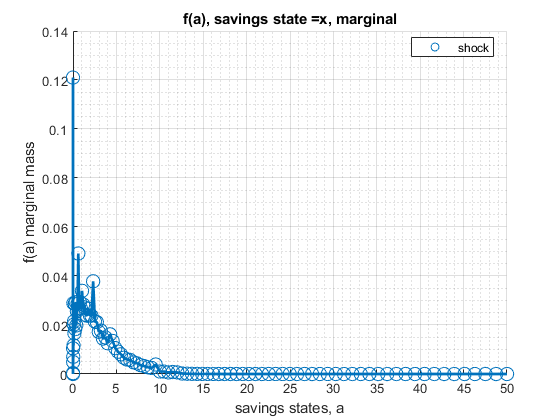
\includegraphics[width=5.20833in,height=\textheight]{img/fx_ds_az_loop_images/figure_0.png}

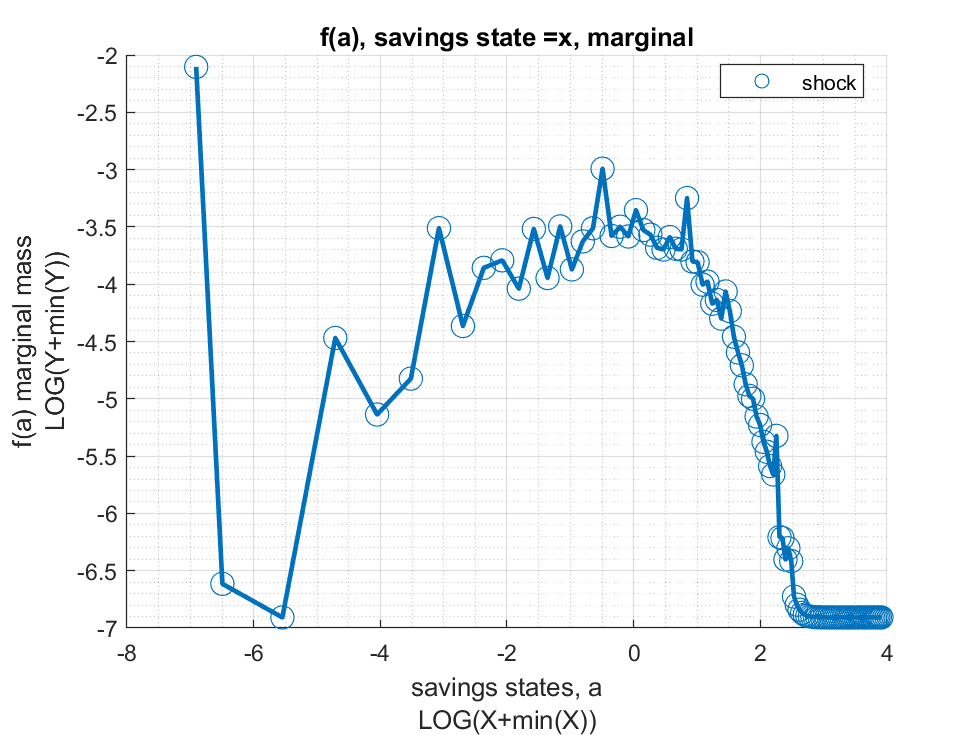
\includegraphics[width=5.20833in,height=\textheight]{img/fx_ds_az_loop_images/figure_1.png}

\hypertarget{test-ff_ds_az_loop-speed-tests}{%
\subsection{Test FF\_DS\_AZ\_LOOP Speed Tests}\label{test-ff_ds_az_loop-speed-tests}}

Call the function with different a and z grid size, print out speed:

\begin{verbatim}
mp_support = containers.Map('KeyType','char', 'ValueType','any');
mp_support('bl_timer') = true;
mp_support('ls_ffcmd') = {};
mp_support('ls_ddcmd') = {};
mp_support('ls_ddgrh') = {};
mp_support('bl_show_stats_table') = false;
% A grid 50, shock grid 5:
mp_params = containers.Map('KeyType','char', 'ValueType','any');
mp_params('it_a_n') = 50;
mp_params('it_z_n') = 5;
ff_ds_az_loop(mp_params, mp_support);

Elapsed time is 0.025627 seconds.
FF_DS_AZ_LOOP finished. Distribution took = 0.066138

% A grid 100, shock grid 7:
mp_params = containers.Map('KeyType','char', 'ValueType','any');
mp_params('it_a_n') = 100;
mp_params('it_z_n') = 7;
ff_ds_az_loop(mp_params, mp_support);

Elapsed time is 0.155714 seconds.
FF_DS_AZ_LOOP finished. Distribution took = 0.11763

% A grid 200, shock grid 9:
mp_params = containers.Map('KeyType','char', 'ValueType','any');
mp_params('it_a_n') = 200;
mp_params('it_z_n') = 9;
ff_ds_az_loop(mp_params, mp_support);

Elapsed time is 0.332056 seconds.
FF_DS_AZ_LOOP finished. Distribution took = 0.32648
\end{verbatim}

\hypertarget{test-ff_ds_az_loop-a-grid-100-shock-grid-7}{%
\subsection{Test FF\_DS\_AZ\_LOOP A grid 100 Shock grid 7}\label{test-ff_ds_az_loop-a-grid-100-shock-grid-7}}

Call the function with different a and z grid size, print out speed:

\begin{verbatim}
mp_support = containers.Map('KeyType','char', 'ValueType','any');
mp_support('bl_timer') = true;
mp_support('ls_ffcmd') = {};
mp_support('ls_ddcmd') = {};
mp_support('ls_ddgrh') = {'faz','fa'};
mp_support('bl_show_stats_table') = true;
mp_params = containers.Map('KeyType','char', 'ValueType','any');
mp_params('it_a_n') = 100;
mp_params('it_z_n') = 7;
ff_ds_az_loop(mp_params, mp_support);

Elapsed time is 0.144655 seconds.
FF_DS_AZ_LOOP finished. Distribution took = 0.13625
\end{verbatim}

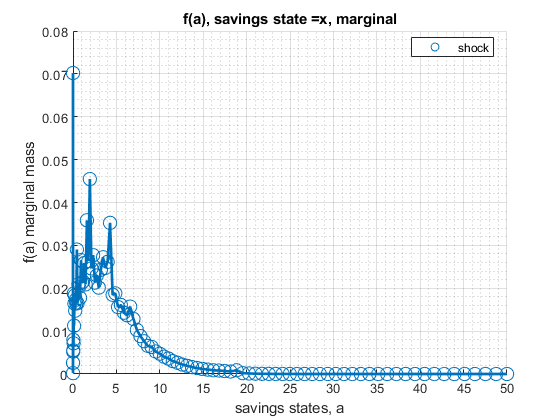
\includegraphics[width=5.20833in,height=\textheight]{img/fx_ds_az_loop_images/figure_2.png}

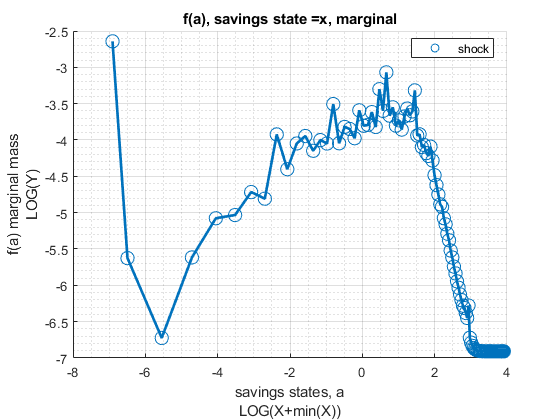
\includegraphics[width=5.20833in,height=\textheight]{img/fx_ds_az_loop_images/figure_3.png}

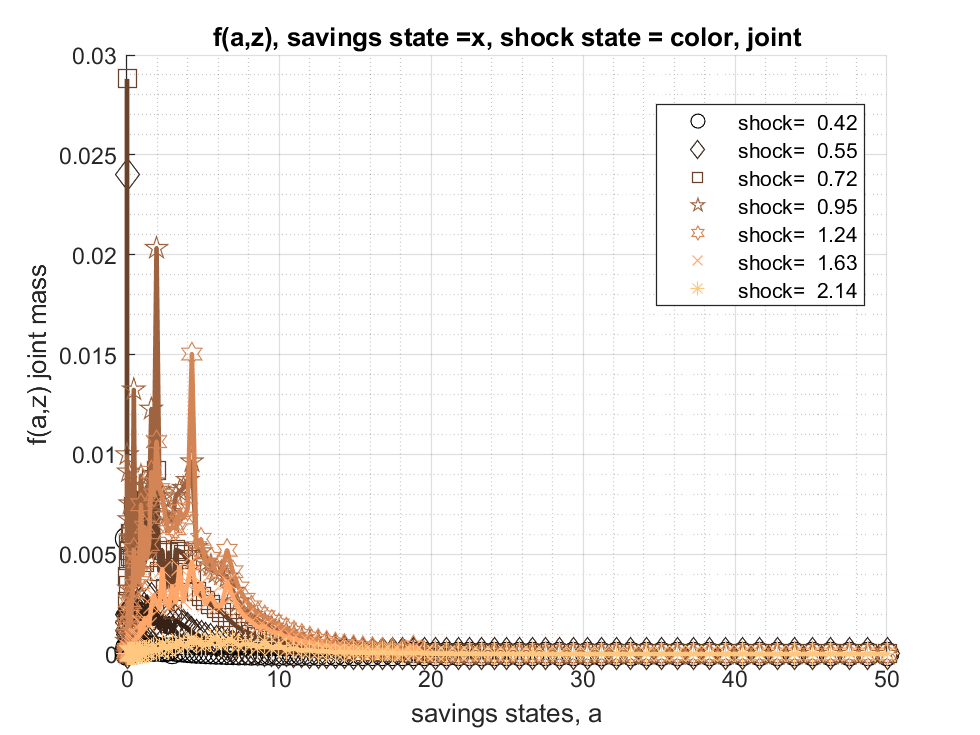
\includegraphics[width=5.20833in,height=\textheight]{img/fx_ds_az_loop_images/figure_4.png}

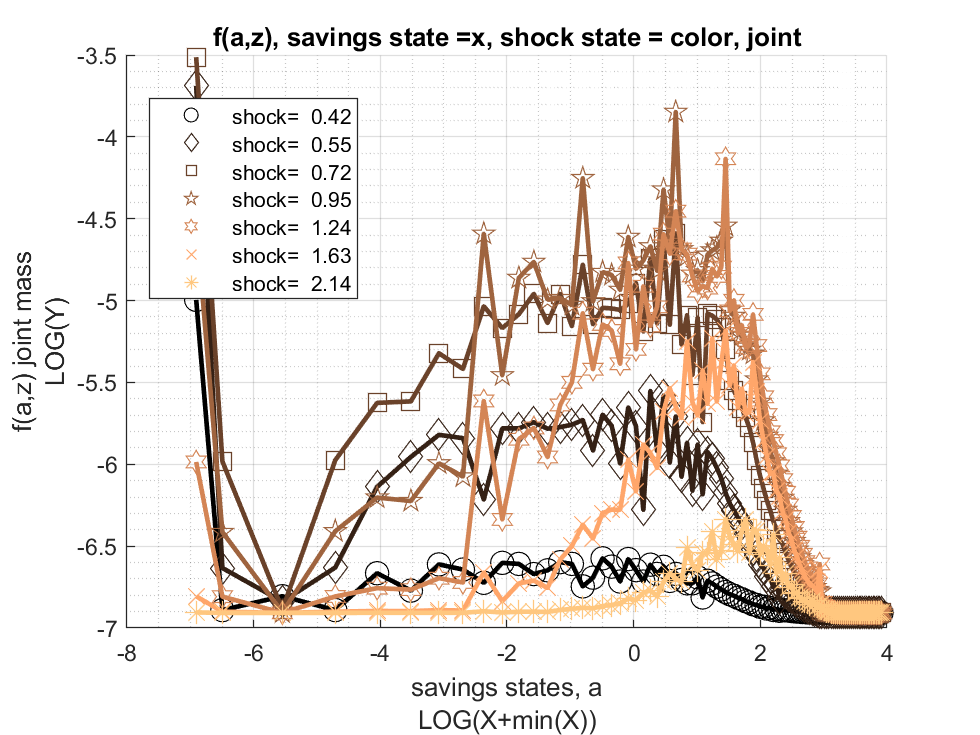
\includegraphics[width=5.20833in,height=\textheight]{img/fx_ds_az_loop_images/figure_5.png}

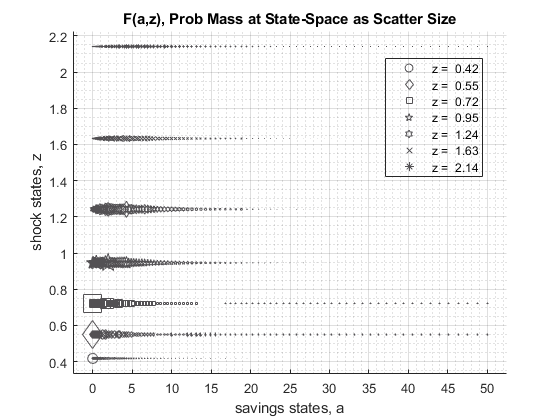
\includegraphics[width=5.20833in,height=\textheight]{img/fx_ds_az_loop_images/figure_6.png}

\begin{verbatim}
xxx tb_outcomes: all stats xxx
    OriginalVariableNames         ap            v             c             y            coh        savefraccoh
    ______________________    __________    __________    __________    __________    __________    ___________

    {'mean'              }        2.7094        6.6576        1.5089        1.5084        4.2183       0.48487 
    {'sd'                }        2.8976        2.0599       0.35843       0.52611        3.2096       0.25477 
    {'coefofvar'         }        1.0694        0.3094       0.23755       0.34879       0.76088       0.52544 
    {'min'               }             0        1.6927       0.58543       0.58543       0.58543             0 
    {'max'               }            50        19.139        4.9969        4.9969        54.997       0.93121 
    {'pYis0'             }      0.070216             0             0             0             0      0.070216 
    {'pYls0'             }             0             0             0             0             0             0 
    {'pYgr0'             }       0.92978             1             1             1             1       0.92978 
    {'pYisMINY'          }      0.070216     0.0057675     0.0057675     0.0057675     0.0057675      0.070216 
    {'pYisMAXY'          }    2.1143e-10    3.7149e-11    3.7149e-11    3.7149e-11    3.7149e-11     2.065e-11 
    {'p0_01'             }             0        1.6927       0.58543       0.58543       0.58543             0 
    {'p0_1'              }             0        1.6927       0.58543       0.58543       0.58543             0 
    {'p1'                }             0        2.7674       0.76855       0.61362       0.76855             0 
    {'p5'                }             0         3.273       0.91608       0.77504         1.009             0 
    {'p10'               }       0.06647        4.0961        1.0308       0.92803        1.1055      0.067651 
    {'p20'               }       0.37601        4.8781        1.2371        1.0319         1.555       0.22796 
    {'p25'               }       0.52503        5.2636        1.2781        1.0731        1.8354       0.28067 
    {'p30'               }        0.7048        5.4822        1.3424        1.1472        2.0866       0.35907 
    {'p40'               }        1.3008        6.0574        1.3953        1.3424        2.6774       0.48584 
    {'p50'               }        1.9422         6.542        1.4931        1.4023        3.3444       0.54915 
    {'p60'               }        2.5275        7.1265        1.6174        1.4954        4.1208       0.60499 
    {'p70'               }         3.456         7.657        1.6502        1.7803        5.1554       0.67918 
    {'p75'               }        3.9869        8.0469         1.733         1.824        5.7555       0.69673 
    {'p80'               }         4.564        8.4125        1.8179        1.8875        6.1793       0.72076 
    {'p90'               }        6.5844        9.3821        1.9734        2.3349         8.568       0.76882 
    {'p95'               }        8.1844        10.225        2.1388        2.4776        10.358       0.80411 
    {'p99'               }        13.136        11.834        2.3359        3.1677        15.511       0.85404 
    {'p99_9'             }        18.839        13.486        2.7733        3.4782        21.332       0.88316 
    {'p99_99'            }        21.778        14.354        3.0939        3.7505         24.78       0.89063 
    {'fl_cov_ap'         }         8.396        5.2587       0.88866       0.93721        9.2847       0.58458 
    {'fl_cor_ap'         }             1       0.88106       0.85565       0.61478       0.99833        0.7919 
    {'fl_cov_v'          }        5.2587         4.243       0.71989       0.93806        5.9786         0.453 
    {'fl_cor_v'          }       0.88106             1       0.97505       0.86559       0.90428       0.86321 
    {'fl_cov_c'          }       0.88866       0.71989       0.12847       0.15253        1.0171      0.079518 
    {'fl_cor_c'          }       0.85565       0.97505             1       0.80886       0.88413        0.8708 
    {'fl_cov_y'          }       0.93721       0.93806       0.15253        0.2768        1.0897      0.080824 
    {'fl_cor_y'          }       0.61478       0.86559       0.80886             1       0.64534         0.603 
    {'fl_cov_coh'        }        9.2847        5.9786        1.0171        1.0897        10.302        0.6641 
    {'fl_cor_coh'        }       0.99833       0.90428       0.88413       0.64534             1       0.81215 
    {'fl_cov_savefraccoh'}       0.58458         0.453      0.079518      0.080824        0.6641      0.064906 
    {'fl_cor_savefraccoh'}        0.7919       0.86321        0.8708         0.603       0.81215             1 
    {'fracByP0_01'       }             0     0.0014664     0.0022377     0.0022385    0.00080043             0 
    {'fracByP0_1'        }             0     0.0014664     0.0022377     0.0022385    0.00080043             0 
    {'fracByP1'          }             0     0.0029302       0.01567       0.00403     0.0055106             0 
    {'fracByP5'          }             0      0.021763      0.026172       0.02466      0.015702             0 
    {'fracByP10'         }     0.0004071      0.050764      0.058937       0.05144      0.022123     0.0021411 
    {'fracByP20'         }     0.0096198        0.1171       0.13549       0.11855       0.05416      0.033082 
    {'fracByP25'         }      0.017608       0.15851       0.17677       0.15694      0.074837      0.057303 
    {'fracByP30'         }       0.02761       0.19906       0.21973       0.19018       0.09783      0.092029 
    {'fracByP40'         }      0.071719       0.28454        0.3135       0.28477       0.15542       0.18016 
    {'fracByP50'         }       0.15388       0.38017       0.40577       0.38385       0.23227       0.28549 
    {'fracByP60'         }       0.21684       0.48325       0.51534       0.46249       0.31381        0.4039 
    {'fracByP70'         }       0.32573       0.59393       0.62048       0.57438       0.42716       0.54543 
    {'fracByP75'         }       0.39815       0.65416       0.68002       0.63899        0.4882       0.60905 
    {'fracByP80'         }       0.48482       0.72413         0.732       0.69931       0.55881        0.6822 
    {'fracByP90'         }        0.6819       0.84902       0.85906        0.8281       0.73338       0.83355 
    {'fracByP95'         }       0.79123       0.91664       0.92592       0.90812       0.83969       0.91574 
    {'fracByP99'         }        0.9433       0.98136       0.98418       0.97889       0.95655       0.98225 
    {'fracByP99_9'       }       0.99595       0.99805       0.99819       0.99776       0.99501       0.99858 
    {'fracByP99_99'      }       0.99934       0.99982       0.99985        0.9998       0.99938       0.99984 
\end{verbatim}

\hypertarget{test-ff_ds_az_loop-a-grid-300-shock-grid-25}{%
\subsection{Test FF\_DS\_AZ\_LOOP A grid 300 Shock Grid 25}\label{test-ff_ds_az_loop-a-grid-300-shock-grid-25}}

\begin{verbatim}
mp_support = containers.Map('KeyType','char', 'ValueType','any');
mp_support('bl_timer') = true;
mp_support('ls_ffcmd') = {};
mp_support('ls_ddcmd') = {};
mp_support('ls_ddgrh') = {'faz','fa'};
mp_support('bl_show_stats_table') = true;
mp_params = containers.Map('KeyType','char', 'ValueType','any');
mp_params('it_a_n') = 300;
mp_params('it_z_n') = 25;
ff_ds_az_loop(mp_params, mp_support);

Elapsed time is 1.664355 seconds.
FF_DS_AZ_LOOP finished. Distribution took = 1.3793
\end{verbatim}

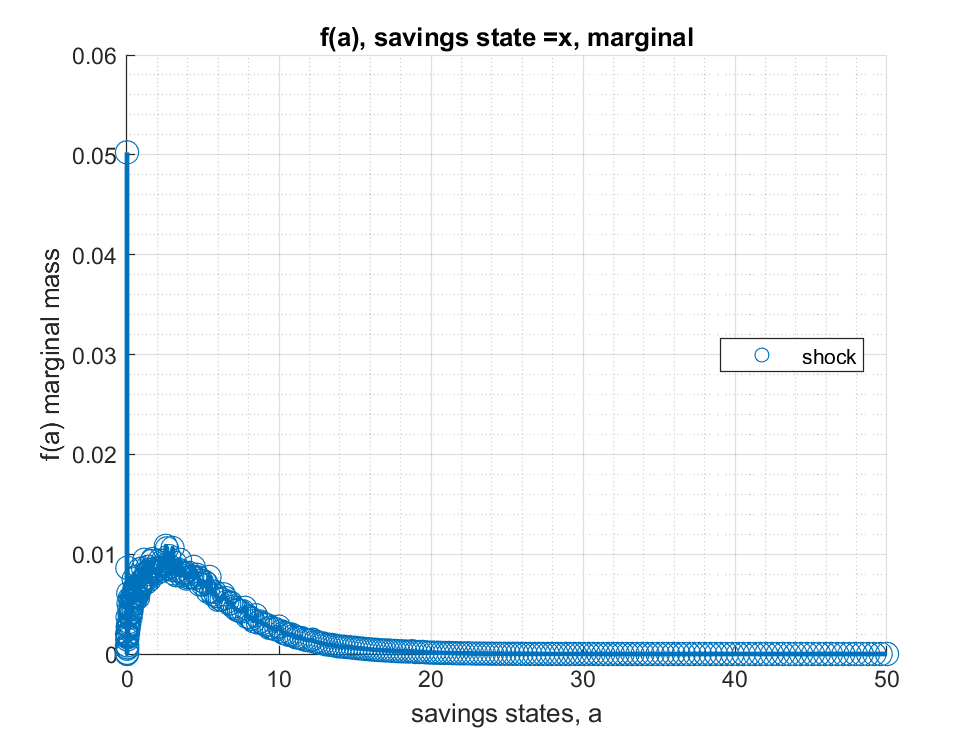
\includegraphics[width=5.20833in,height=\textheight]{img/fx_ds_az_loop_images/figure_7.png}

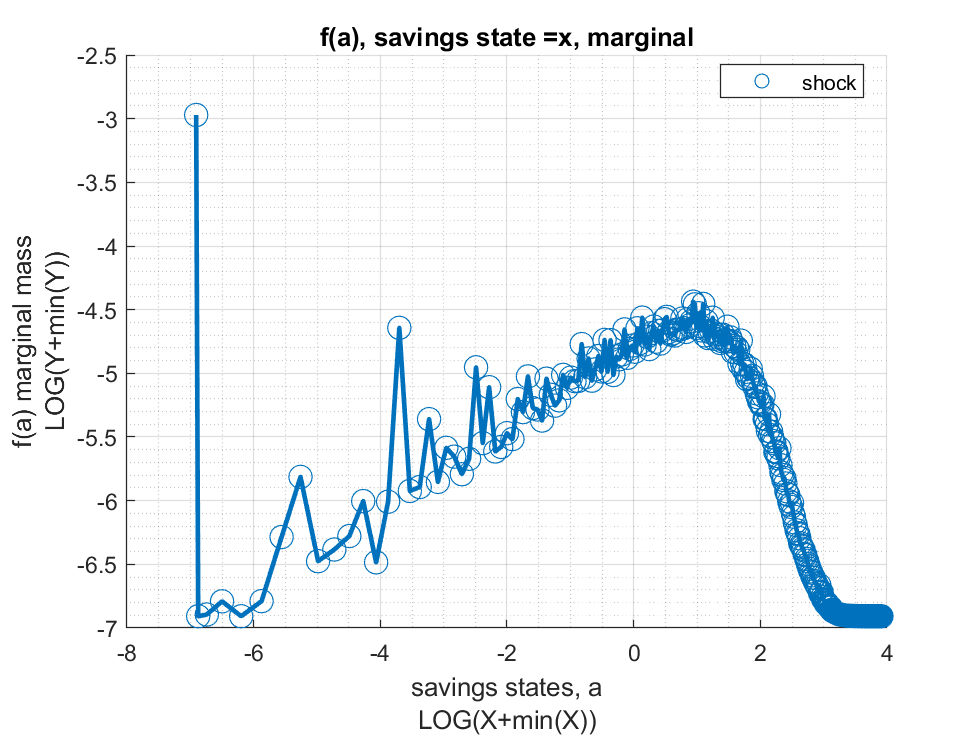
\includegraphics[width=5.20833in,height=\textheight]{img/fx_ds_az_loop_images/figure_8.png}

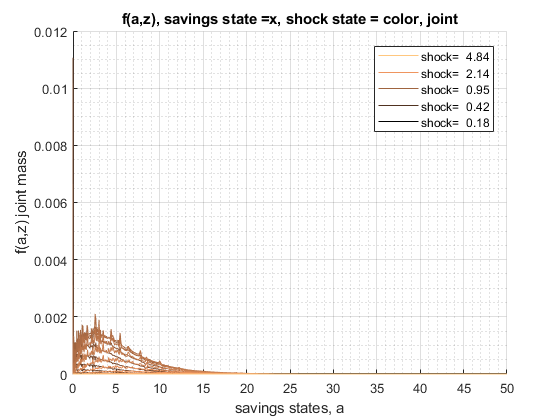
\includegraphics[width=5.20833in,height=\textheight]{img/fx_ds_az_loop_images/figure_9.png}

\includegraphics[width=5.20833in,height=\textheight]{img/fx_ds_az_loop_images/figure_10.png}

\includegraphics[width=5.20833in,height=\textheight]{img/fx_ds_az_loop_images/figure_11.png}

\begin{verbatim}
xxx tb_outcomes: all stats xxx
    OriginalVariableNames         ap            v             c             y            coh        savefraccoh
    ______________________    __________    __________    __________    __________    __________    ___________

    {'mean'              }        3.1835        6.9106        1.5286        1.5274        4.7121       0.52236 
    {'sd'                }        3.2831         2.152       0.35175       0.53521        3.5973       0.25161 
    {'coefofvar'         }        1.0313       0.31141        0.2301       0.35041       0.76341       0.48168 
    {'min'               }             0       -2.7621       0.25871       0.25871       0.25871             0 
    {'max'               }            50        20.027        8.7798        8.7798         58.78       0.93152 
    {'pYis0'             }      0.050267             0             0             0             0      0.050267 
    {'pYls0'             }             0    7.4299e-05             0             0             0             0 
    {'pYgr0'             }       0.94973       0.99993             1             1             1       0.94973 
    {'pYisMINY'          }      0.050267    3.1587e-08    3.1587e-08    3.1587e-08    3.1587e-08      0.050267 
    {'pYisMAXY'          }    2.3964e-09    9.6288e-14    9.6288e-14    9.6288e-14    9.6288e-14    2.6173e-22 
    {'p0_01'             }             0       0.33524       0.44588       0.42089       0.44588             0 
    {'p0_1'              }             0        1.0281       0.51088       0.51088       0.51088             0 
    {'p1'                }             0        2.3294       0.67069       0.67069       0.67069             0 
    {'p5'                }             0         3.531        0.9348       0.80006        1.0088             0 
    {'p10'               }       0.10107        4.1808        1.0877       0.90775        1.2209      0.086874 
    {'p20'               }       0.48982        5.0629         1.248        1.0638        1.7564       0.28154 
    {'p25'               }        0.7256        5.3749        1.3048         1.157        2.0452       0.35473 
    {'p30'               }       0.97897        5.7085        1.3561         1.192        2.3425        0.4186 
    {'p40'               }        1.5756        6.2702        1.4389        1.3331        2.9951       0.51678 
    {'p50'               }        2.2184        6.8025        1.5235        1.4352        3.7422       0.59639 
    {'p60'               }        2.9972        7.3608        1.6237        1.5724        4.6044       0.65168 
    {'p70'               }         4.012         7.977        1.7017        1.7487        5.6899        0.7051 
    {'p75'               }        4.5871        8.3254        1.7349        1.8191        6.3522       0.72563 
    {'p80'               }        5.3173        8.7116        1.8227        1.9222        7.1504       0.74857 
    {'p90'               }        7.5009        9.7584        1.9829        2.2334         9.526       0.79537 
    {'p95'               }        9.6743        10.633        2.1133        2.5088        11.809       0.82382 
    {'p99'               }        14.854        12.286        2.3901        3.1545        17.176       0.86207 
    {'p99_9'             }        21.166        14.023        2.7913        3.9726        23.779       0.88709 
    {'p99_99'            }        26.803        15.357        3.0931        4.7968        29.914       0.89989 
    {'fl_cov_ap'         }        10.779        6.2944         1.019        1.0643        11.798       0.64446 
    {'fl_cor_ap'         }             1       0.89089       0.88234       0.60566       0.99894       0.78015 
    {'fl_cov_v'          }        6.2944        4.6311        0.7528       0.97564        7.0472       0.46366 
    {'fl_cor_v'          }       0.89089             1        0.9945       0.84708       0.91033       0.85631 
    {'fl_cov_c'          }         1.019        0.7528       0.12373       0.15568        1.1427      0.077608 
    {'fl_cor_c'          }       0.88234        0.9945             1       0.82696       0.90306        0.8769 
    {'fl_cov_y'          }        1.0643       0.97564       0.15568       0.28645        1.2199      0.077311 
    {'fl_cor_y'          }       0.60566       0.84708       0.82696             1       0.63363       0.57411 
    {'fl_cov_coh'        }        11.798        7.0472        1.1427        1.2199        12.941       0.72207 
    {'fl_cor_coh'        }       0.99894       0.91033       0.90306       0.63363             1       0.79776 
    {'fl_cov_savefraccoh'}       0.64446       0.46366      0.077608      0.077311       0.72207      0.063308 
    {'fl_cor_savefraccoh'}       0.78015       0.85631        0.8769       0.57411       0.79776             1 
    {'fracByP0_01'       }             0     7.366e-06    9.1288e-05    2.5324e-05    2.9613e-05             0 
    {'fracByP0_1'        }             0    0.00015226    0.00040756    0.00048297    0.00013202             0 
    {'fracByP1'          }             0     0.0031657     0.0040997     0.0058265     0.0013172             0 
    {'fracByP5'          }             0      0.020854      0.026015      0.023308      0.010613             0 
    {'fracByP10'         }     0.0007829      0.049187      0.059665      0.051833      0.020313     0.0040897 
    {'fracByP20'         }      0.010458        0.1169       0.13673       0.11782      0.052147       0.04121 
    {'fracByP25'         }      0.020375       0.15489       0.17838       0.15407      0.072616      0.071271 
    {'fracByP30'         }      0.033945       0.19501       0.22212        0.1924       0.09561       0.10878 
    {'fracByP40'         }      0.076084       0.28102        0.3131        0.2752       0.15182       0.19951 
    {'fracByP50'         }       0.13323        0.3766       0.41016       0.36618       0.22332       0.30599 
    {'fracByP60'         }       0.21876        0.4783       0.51311       0.46472       0.31143       0.42495 
    {'fracByP70'         }       0.32789       0.58936       0.62182       0.57246        0.4201       0.55532 
    {'fracByP75'         }       0.39329       0.64823       0.67676       0.63063       0.48449       0.62358 
    {'fracByP80'         }       0.47094       0.70976       0.73532       0.69204       0.55555         0.694 
    {'fracByP90'         }       0.66575       0.84269       0.85851       0.82742       0.72907       0.84261 
    {'fracByP95'         }        0.8001       0.91584       0.92543       0.90488       0.84038       0.91895 
    {'fracByP99'         }       0.94734       0.98115       0.98337       0.97713       0.95746       0.98325 
    {'fracByP99_9'       }       0.99324       0.99789       0.99809       0.99717       0.99445        0.9983 
    {'fracByP99_99'      }       0.99909       0.99977       0.99979       0.99967       0.99931       0.99983 
\end{verbatim}

\hypertarget{test-ff_ds_az_loop-a-grid-300-shock-grid-50}{%
\subsection{Test FF\_DS\_AZ\_LOOP A grid 300 Shock Grid 50}\label{test-ff_ds_az_loop-a-grid-300-shock-grid-50}}

\begin{verbatim}
mp_support = containers.Map('KeyType','char', 'ValueType','any');
mp_support('bl_timer') = true;
mp_support('ls_ffcmd') = {};
mp_support('ls_ddcmd') = {};
mp_support('ls_ddgrh') = {'faz','fa'};
mp_support('bl_show_stats_table') = true;
mp_params = containers.Map('KeyType','char', 'ValueType','any');
mp_params('it_a_n') = 300;
mp_params('it_z_n') = 50;
ff_ds_az_loop(mp_params, mp_support);

Elapsed time is 4.319877 seconds.
FF_DS_AZ_LOOP finished. Distribution took = 3.0884
\end{verbatim}

\includegraphics[width=5.20833in,height=\textheight]{img/fx_ds_az_loop_images/figure_12.png}

\includegraphics[width=5.20833in,height=\textheight]{img/fx_ds_az_loop_images/figure_13.png}

\includegraphics[width=5.20833in,height=\textheight]{img/fx_ds_az_loop_images/figure_14.png}

\includegraphics[width=5.20833in,height=\textheight]{img/fx_ds_az_loop_images/figure_15.png}

\includegraphics[width=5.20833in,height=\textheight]{img/fx_ds_az_loop_images/figure_16.png}

\begin{verbatim}
xxx tb_outcomes: all stats xxx
    OriginalVariableNames         ap            v             c             y            coh        savefraccoh
    ______________________    __________    __________    __________    __________    __________    ___________

    {'mean'              }          3.26        6.9484        1.5319        1.5305        4.7919       0.52772 
    {'sd'                }        3.3166        2.1606       0.35167        0.5364        3.6315       0.25217 
    {'coefofvar'         }        1.0174       0.31094       0.22956       0.35048       0.75783       0.47785 
    {'min'               }             0       -7.6871       0.12843       0.12843       0.12843             0 
    {'max'               }            50        20.751        15.657        15.657        65.657       0.93164 
    {'pYis0'             }      0.049546             0             0             0             0      0.049546 
    {'pYls0'             }             0    0.00011924             0             0             0             0 
    {'pYgr0'             }       0.95045       0.99988             1             1             1       0.95045 
    {'pYisMINY'          }      0.049546    1.1021e-15    1.1021e-15    1.1021e-15    1.1021e-15      0.049546 
    {'pYisMAXY'          }    5.1436e-09    3.0978e-19    3.0978e-19    3.0978e-19    3.0978e-19    7.4151e-23 
    {'p0_01'             }             0      -0.20486       0.40271       0.40271       0.40271             0 
    {'p0_1'              }             0        1.2135       0.53589         0.488       0.53589             0 
    {'p1'                }             0        2.3687       0.71312       0.64833       0.71312             0 
    {'p5'                }    0.00050419        3.5428       0.94895        0.8071       0.96945    0.00055062 
    {'p10'               }       0.11149        4.2401        1.0944       0.93681        1.2484      0.095151 
    {'p20'               }       0.51629        5.0791         1.255         1.072        1.7729       0.28687 
    {'p25'               }       0.75904        5.4237        1.3033        1.1504         2.067       0.36257 
    {'p30'               }        1.0189        5.7339        1.3518        1.2006        2.3841       0.42942 
    {'p40'               }        1.6286        6.2919         1.446        1.3198        3.0593       0.53021 
    {'p50'               }        2.2834        6.8389        1.5355        1.4423        3.8053       0.59978 
    {'p60'               }        3.0751        7.4137         1.613        1.5765        4.7113       0.65858 
    {'p70'               }        4.1046        8.0318        1.7011        1.7318        5.8286       0.70939 
    {'p75'               }        4.7891        8.3723        1.7435        1.8266        6.5055       0.73443 
    {'p80'               }        5.5379         8.765        1.8035        1.9295        7.3201       0.75699 
    {'p90'               }        7.6355        9.7879        1.9921        2.2457        9.6214       0.79808 
    {'p95'               }        9.8311         10.68        2.1096        2.5308        11.976       0.82663 
    {'p99'               }        14.653        12.305         2.407        3.1554        17.087       0.86199 
    {'p99_9'             }        21.166        14.067        2.7771        4.0255        23.953       0.88705 
    {'p99_99'            }        27.382        15.467        3.1325         4.887        30.554       0.90105 
    {'fl_cov_ap'         }            11        6.3988         1.032        1.0771        12.032       0.65387 
    {'fl_cor_ap'         }             1       0.89298       0.88481       0.60546       0.99898       0.78182 
    {'fl_cov_v'          }        6.3988         4.668       0.75538       0.97839        7.1542       0.46619 
    {'fl_cor_v'          }       0.89298             1       0.99418       0.84423       0.91183       0.85567 
    {'fl_cov_c'          }         1.032       0.75538       0.12367       0.15613        1.1557      0.077331 
    {'fl_cor_c'          }       0.88481       0.99418             1       0.82768       0.90493       0.87203 
    {'fl_cov_y'          }        1.0771       0.97839       0.15613       0.28772        1.2333      0.076912 
    {'fl_cor_y'          }       0.60546       0.84423       0.82768             1       0.63312       0.56861 
    {'fl_cov_coh'        }        12.032        7.1542        1.1557        1.2333        13.188        0.7312 
    {'fl_cor_coh'        }       0.99898       0.91183       0.90493       0.63312             1       0.79848 
    {'fl_cov_savefraccoh'}       0.65387       0.46619      0.077331      0.076912        0.7312      0.063589 
    {'fl_cor_savefraccoh'}       0.78182       0.85567       0.87203       0.56861       0.79848             1 
    {'fracByP0_01'       }             0    -7.082e-06    2.6291e-05    3.0744e-05    8.4044e-06             0 
    {'fracByP0_1'        }             0    8.1705e-05    0.00058298    0.00029929    0.00018591             0 
    {'fracByP1'          }             0     0.0025872     0.0055744     0.0043199     0.0017463             0 
    {'fracByP5'          }    5.9482e-08       0.02063      0.028475      0.023256     0.0085179    3.9707e-07 
    {'fracByP10'         }    0.00083251      0.049013      0.059787      0.051875      0.020182      0.004399 
    {'fracByP20'         }       0.01069       0.11692       0.13707       0.11785      0.051473      0.041367 
    {'fracByP25'         }      0.021006       0.15459       0.17869       0.15432      0.071586      0.072106 
    {'fracByP30'         }      0.034297       0.19493       0.22235       0.19226      0.095063       0.10998 
    {'fracByP40'         }      0.076942        0.2811       0.31433       0.27537       0.15173       0.20135 
    {'fracByP50'         }       0.13547       0.37553       0.41049       0.36597       0.22294       0.30799 
    {'fracByP60'         }       0.21688       0.47822       0.51321       0.46464       0.31179       0.42743 
    {'fracByP70'         }       0.32617       0.58918        0.6213       0.57279       0.42106       0.55684 
    {'fracByP75'         }       0.40001       0.64825       0.67795        0.6311       0.48455       0.62544 
    {'fracByP80'         }       0.47816       0.71036       0.73507       0.69272       0.55654       0.69664 
    {'fracByP90'         }       0.67319       0.84299       0.85862       0.82739       0.73089       0.84294 
    {'fracByP95'         }       0.80347       0.91616       0.92515       0.90483       0.84244       0.91987 
    {'fracByP99'         }       0.94675       0.98117       0.98325       0.97691       0.95831       0.98345 
    {'fracByP99_9'       }       0.99284       0.99789        0.9981       0.99713       0.99445       0.99831 
    {'fracByP99_99'      }       0.99909       0.99977       0.99979       0.99966        0.9993       0.99983
\end{verbatim}

\hypertarget{ff_ds_az_cts_loop-dynamic-savings-loop-continuous-distribution}{%
\section{FF\_DS\_AZ\_CTS\_LOOP Dynamic Savings Loop Continuous Distribution}\label{ff_ds_az_cts_loop-dynamic-savings-loop-continuous-distribution}}

\begin{quote}
Go back to \href{http://fanwangecon.github.io/}{fan}'s \href{https://fanwangecon.github.io/MEconTools/}{MEconTools} Toolbox (\href{https://fanwangecon.github.io/MEconTools/bookdown}{bookdown}), \href{https://fanwangecon.github.io/M4Econ/}{Matlab Code Examples} Repository (\href{https://fanwangecon.github.io/M4Econ/bookdown}{bookdown}), or \href{https://fanwangecon.github.io/Math4Econ/}{Math for Econ with Matlab} Repository (\href{https://fanwangecon.github.io/Math4Econ/bookdown}{bookdown}).
\end{quote}

This is the example vignette for function:
\href{https://github.com/FanWangEcon/MEconTools/blob/master/MEconTools/vfi/ff_ds_az_cts_loop.m}{\textbf{ff\_ds\_az\_cts\_loop}}
from the \href{https://fanwangecon.github.io/MEconTools/}{\textbf{MEconTools
Package}}\textbf{.} F(a,z)
discrete probability mass function given policy function solution with
continuous savings choices.

\begin{itemize}
\item
  Distribution for Common Choice and States Grid :
  ff\_ds\_az\_cts\_loop
\item
  Distribution for States Grid + Continuous Exact Savings as Share of
  Cash-on-Hand :
  \href{https://github.com/FanWangEcon/MEconTools/blob/master/MEconTools/vfi/ff_ds_az_cts_loop.m}{\textbf{ff\_ds\_az\_cts\_loop}}
\end{itemize}

\hypertarget{test-ff_ds_az_cts_loop-defaults}{%
\subsection{Test FF\_DS\_AZ\_CTS\_LOOP Defaults}\label{test-ff_ds_az_cts_loop-defaults}}

Call the function with defaults. By default, shows the asset policy
function summary. Model parameters can be changed by the mp\_params.

\begin{verbatim}
%mp_params
mp_params = containers.Map('KeyType','char', 'ValueType','any');
mp_params('fl_crra') = 1.5;
mp_params('fl_beta') = 0.94;
% call function
ff_ds_az_cts_loop(mp_params);

Elapsed time is 1.029654 seconds.
----------------------------------------
xxxxxxxxxxxxxxxxxxxxxxxxxxxxxxxxxxxxxxxx
CONTAINER NAME: mp_ffcmd ND Array (Matrix etc)
xxxxxxxxxxxxxxxxxxxxxxxxxxxxxxxxxxxxxxxx
          i    idx    ndim    numel    rowN    colN     sum       mean      std      coefvari    min     max  
          _    ___    ____    _____    ____    ____    ______    ______    ______    ________    ___    ______

    ap    1     1      2       700     100      7      9863.4    14.091    14.388     1.0211      0     50.117

xxx TABLE:ap xxxxxxxxxxxxxxxxxx
              c1        c2        c3         c4         c5         c6         c7  
            ______    ______    ______    ________    _______    _______    ______

    r1           0         0         0    0.053491    0.25574    0.60604    1.1157
    r2           0         0         0    0.053998    0.25571     0.6066    1.1163
    r3           0         0         0    0.056449    0.25576    0.60907    1.1187
    r4           0         0         0    0.061799    0.26016     0.6109    1.1239
    r5           0         0         0    0.066463    0.26897    0.61141    1.1327
    r96     43.388     43.52    43.701      43.925     44.222      44.68    45.228
    r97     44.566    44.695    44.878      45.103     45.398     45.856    46.403
    r98     45.761    45.892    46.072      46.298     46.592      47.05    47.597
    r99     46.973    47.107    47.286      47.514     47.806     48.263    48.815
    r100    48.206    48.338    48.519      48.746     49.037     49.497    50.117

FF_DS_AZ_CTS_LOOP finished. Distribution took = 0.25795
----------------------------------------
xxxxxxxxxxxxxxxxxxxxxxxxxxxxxxxxxxxxxxxx
CONTAINER NAME: mp_ddcmd ND Array (Matrix etc)
xxxxxxxxxxxxxxxxxxxxxxxxxxxxxxxxxxxxxxxx
           i    idx    ndim    numel    rowN    colN    sum      mean         std       coefvari       min          max  
           _    ___    ____    _____    ____    ____    ___    _________    ________    ________    __________    _______

    fa     1     1      2       100     100      1       1          0.01      0.0155       1.55     2.6966e-22    0.11839
    faz    2     2      2       700     100      7       1     0.0014286    0.003424     2.3968     1.9078e-27    0.05152
    fz     3     3      2         7       7      1       1       0.14286     0.11742    0.82196       0.015625     0.3125

xxx TABLE:fa xxxxxxxxxxxxxxxxxx
                c1    
            __________

    r1         0.11839
    r2      0.00028039
    r3      2.8585e-05
    r4       0.0082178
    r5       0.0062146
    r96     1.3607e-18
    r97     2.0727e-19
    r98     2.7005e-20
    r99     2.9248e-21
    r100    2.6966e-22

xxx TABLE:faz xxxxxxxxxxxxxxxxxx
                c1            c2            c3            c4            c5            c6            c7    
            __________    __________    __________    __________    __________    __________    __________

    r1       0.0082492      0.036999       0.05152      0.018557     0.0028578    0.00020313    5.5014e-06
    r2      0.00014901     9.934e-05    2.7594e-05     4.088e-06    3.4067e-07    1.5141e-08    2.8039e-10
    r3      1.0791e-06    3.8554e-06     1.588e-05    6.6114e-06    1.0779e-06    7.8977e-08    2.1795e-09
    r4      0.00016483     0.0019292      0.004208     0.0016366    0.00025991    1.8779e-05    5.1379e-07
    r5      0.00019509    0.00082304     0.0034877     0.0014538    0.00023711    1.7374e-05     4.795e-07
    r96     4.1576e-23    1.0459e-21    1.1798e-20    7.4995e-20    2.7503e-19    5.3901e-19    4.5877e-19
    r97     5.3415e-24    1.4108e-22    1.6619e-21    1.0943e-20    4.1203e-20    8.2324e-20    7.0996e-20
    r98      5.734e-25    1.6065e-23    1.9875e-22    1.3596e-21    5.2668e-21     1.075e-20     9.414e-21
    r99     4.7136e-26    1.4644e-24    1.9531e-23    1.4042e-22    5.6108e-22    1.1675e-21    1.0348e-21
    r100    1.9078e-27    7.8348e-26    1.2906e-24    1.0816e-23    4.8188e-23    1.0831e-22    1.0098e-22

xxx TABLE:fz xxxxxxxxxxxxxxxxxx
             c1   
          ________

    r1    0.015625
    r2     0.09375
    r3     0.23438
    r4      0.3125
    r5     0.23438
    r6     0.09375
    r7    0.015625
\end{verbatim}

\includegraphics[width=5.20833in,height=\textheight]{img/fx_ds_az_cts_loop_images/figure_0.png}

\includegraphics[width=5.20833in,height=\textheight]{img/fx_ds_az_cts_loop_images/figure_1.png}

\begin{verbatim}
xxx tb_outcomes: all stats xxx
    OriginalVariableNames         ap            v             c             y            coh        savefraccoh
    ______________________    __________    __________    __________    __________    __________    ___________

    {'mean'              }        1.6576        5.0855        1.4665        1.4663        3.1241       0.37319 
    {'sd'                }        1.9603        1.7128         0.362       0.51116        2.2726       0.24899 
    {'coefofvar'         }        1.1826       0.33679       0.24684        0.3486       0.72744       0.66717 
    {'min'               }             0       0.87463       0.58543       0.58543       0.58543             0 
    {'max'               }        50.117        16.344        4.8795        4.9969        54.997       0.91671 
    {'pYis0'             }        0.1184             0             0             0             0        0.1184 
    {'pYls0'             }             0             0             0             0             0             0 
    {'pYgr0'             }        0.8816             1             1             1             1        0.8816 
    {'pYisMINY'          }        0.1184     0.0082492     0.0082492     0.0082492     0.0082492        0.1184 
    {'pYisMAXY'          }    1.0098e-22    1.0098e-22    1.0098e-22    1.0098e-22    1.0098e-22    1.9078e-27 
    {'p0_01'             }             0       0.87463       0.58543       0.58543       0.58543             0 
    {'p0_1'              }             0       0.87463       0.58543       0.58543       0.58543             0 
    {'p1'                }             0        1.1243       0.69861       0.59041         0.715             0 
    {'p5'                }             0        2.0791       0.77687       0.76855       0.78562             0 
    {'p10'               }             0        3.1895         1.009       0.85364         1.009             0 
    {'p20'               }        0.1057        3.4752          1.14        1.0154        1.3246      0.087685 
    {'p25'               }        0.1939        3.8676        1.2593        1.0372        1.4541       0.14292 
    {'p30'               }       0.31246        4.2445         1.288        1.0797        1.5906       0.19132 
    {'p40'               }       0.60724        4.5309        1.3707        1.3296        1.9628       0.29984 
    {'p50'               }       0.95427         5.055        1.4829        1.3613        2.4022       0.39725 
    {'p60'               }        1.4469        5.5086        1.5637        1.4343        2.9909       0.48624 
    {'p70'               }        2.0596        5.9381        1.6462        1.7599        3.7395       0.55313 
    {'p75'               }        2.4165        6.2179        1.7114        1.7855        4.1539       0.58951 
    {'p80'               }        2.8138        6.5733        1.7777         1.824        4.6604       0.62436 
    {'p90'               }        4.2696        7.3417        1.9216         2.311        6.1793       0.69436 
    {'p95'               }        5.8173        8.0019        2.0504        2.4211        7.7898       0.74197 
    {'p99'               }        8.6172        9.1635        2.3145        3.1157        10.795       0.79263 
    {'p99_9'             }        12.332         10.32        2.5888        3.3595        14.819        0.8312 
    {'p99_99'            }        15.614        11.187        2.8357        3.5223        18.494        0.8503 
    {'fl_cov_ap'         }        3.8427        2.8209       0.59546       0.62646        4.4381       0.41171 
    {'fl_cor_ap'         }             1       0.84018       0.83914        0.6252       0.99624       0.84353 
    {'fl_cov_v'          }        2.8209        2.9336       0.61788       0.78698        3.4388       0.36784 
    {'fl_cor_v'          }       0.84018             1       0.99656        0.8989       0.88346       0.86257 
    {'fl_cov_c'          }       0.59546       0.61788       0.13104       0.16288        0.7265      0.079955 
    {'fl_cor_c'          }       0.83914       0.99656             1       0.88023       0.88311       0.88709 
    {'fl_cov_y'          }       0.62646       0.78698       0.16288       0.26129       0.78934      0.080066 
    {'fl_cor_y'          }        0.6252        0.8989       0.88023             1       0.67949       0.62909 
    {'fl_cov_coh'        }        4.4381        3.4388        0.7265       0.78934        5.1646       0.49166 
    {'fl_cor_coh'        }       0.99624       0.88346       0.88311       0.67949             1       0.86891 
    {'fl_cov_savefraccoh'}       0.41171       0.36784      0.079955      0.080066       0.49166      0.061994 
    {'fl_cor_savefraccoh'}       0.84353       0.86257       0.88709       0.62909       0.86891             1 
    {'fracByP0_01'       }             0     0.0014187      0.003293     0.0032935     0.0015458             0 
    {'fracByP0_1'        }             0     0.0014187      0.003293     0.0032935     0.0015458             0 
    {'fracByP1'          }             0        0.0018     0.0041476     0.0040773     0.0019486             0 
    {'fracByP5'          }             0      0.017798      0.025084      0.025722      0.011837             0 
    {'fracByP10'         }             0      0.069566      0.076643      0.051708      0.032927             0 
    {'fracByP20'         }     0.0028528        0.1122       0.13024        0.1217      0.065169      0.011916 
    {'fracByP25'         }     0.0077609       0.14388       0.17442       0.15825      0.090199      0.025805 
    {'fracByP30'         }      0.016336        0.1847       0.21519        0.1908       0.11027      0.047181 
    {'fracByP40'         }      0.044743       0.27669       0.31043       0.27733       0.16769       0.11744 
    {'fracByP50'         }      0.091661       0.37143       0.40445       0.37462        0.2384       0.21415 
    {'fracByP60'         }        0.1676       0.47128       0.50501       0.46524       0.33103       0.33325 
    {'fracByP70'         }       0.27323       0.58248        0.6172       0.57522       0.43968       0.47636 
    {'fracByP75'         }       0.33601       0.64052       0.67429       0.63346       0.50276       0.54669 
    {'fracByP80'         }       0.41177       0.70413       0.73317       0.69614       0.57118       0.62562 
    {'fracByP90'         }       0.62757       0.84178       0.85697       0.82738       0.73915       0.80081 
    {'fracByP95'         }       0.77414        0.9151       0.92509       0.91117       0.84868       0.89896 
    {'fracByP99'         }        0.9381       0.98132       0.98368       0.97823        0.9596       0.97843 
    {'fracByP99_9'       }       0.99212       0.99801       0.99826       0.99811       0.99474       0.99783 
    {'fracByP99_99'      }       0.99909        0.9998       0.99982       0.99981       0.99944       0.99978 
\end{verbatim}

\hypertarget{test-ff_ds_az_cts_loop-speed-tests}{%
\subsection{Test FF\_DS\_AZ\_CTS\_LOOP Speed Tests}\label{test-ff_ds_az_cts_loop-speed-tests}}

Call the function with different a and z grid size, print out speed:

\begin{verbatim}
mp_support = containers.Map('KeyType','char', 'ValueType','any');
mp_support('bl_timer') = true;
mp_support('ls_ffcmd') = {};
mp_support('ls_ddcmd') = {};
mp_support('ls_ddgrh') = {};
mp_support('bl_show_stats_table') = false;
% A grid 50, shock grid 5:
mp_params = containers.Map('KeyType','char', 'ValueType','any');
mp_params('it_a_n') = 50;
mp_params('it_z_n') = 5;
ff_ds_az_cts_loop(mp_params, mp_support);

Elapsed time is 0.610510 seconds.
FF_DS_AZ_CTS_LOOP finished. Distribution took = 0.081975

% A grid 100, shock grid 7:
mp_params = containers.Map('KeyType','char', 'ValueType','any');
mp_params('it_a_n') = 100;
mp_params('it_z_n') = 7;
ff_ds_az_cts_loop(mp_params, mp_support);

Elapsed time is 1.114978 seconds.
FF_DS_AZ_CTS_LOOP finished. Distribution took = 0.18449

% A grid 200, shock grid 9:
mp_params = containers.Map('KeyType','char', 'ValueType','any');
mp_params('it_a_n') = 200;
mp_params('it_z_n') = 9;
ff_ds_az_cts_loop(mp_params, mp_support);

Elapsed time is 2.014970 seconds.
FF_DS_AZ_CTS_LOOP finished. Distribution took = 0.62806
\end{verbatim}

\hypertarget{test-ff_ds_az_cts_loop-a-grid-100-shock-grid-7}{%
\subsection{Test FF\_DS\_AZ\_CTS\_LOOP A grid 100 Shock grid 7}\label{test-ff_ds_az_cts_loop-a-grid-100-shock-grid-7}}

Call the function with different a and z grid size, print out speed:

\begin{verbatim}
mp_support = containers.Map('KeyType','char', 'ValueType','any');
mp_support('bl_timer') = true;
mp_support('ls_ffcmd') = {};
mp_support('ls_ddcmd') = {};
mp_support('ls_ddgrh') = {'faz','fa'};
mp_support('bl_show_stats_table') = true;
mp_params = containers.Map('KeyType','char', 'ValueType','any');
mp_params('it_a_n') = 100;
mp_params('it_z_n') = 7;
ff_ds_az_cts_loop(mp_params, mp_support);

Elapsed time is 0.953345 seconds.
FF_DS_AZ_CTS_LOOP finished. Distribution took = 0.23426
\end{verbatim}

\includegraphics[width=5.20833in,height=\textheight]{img/fx_ds_az_cts_loop_images/figure_2.png}

\includegraphics[width=5.20833in,height=\textheight]{img/fx_ds_az_cts_loop_images/figure_3.png}

\includegraphics[width=5.20833in,height=\textheight]{img/fx_ds_az_cts_loop_images/figure_4.png}

\includegraphics[width=5.20833in,height=\textheight]{img/fx_ds_az_cts_loop_images/figure_5.png}

\includegraphics[width=5.20833in,height=\textheight]{img/fx_ds_az_cts_loop_images/figure_6.png}

\begin{verbatim}
xxx tb_outcomes: all stats xxx
    OriginalVariableNames         ap            v             c             y            coh        savefraccoh
    ______________________    __________    __________    __________    __________    __________    ___________

    {'mean'              }        3.2216        6.9329        1.5295        1.5289        4.7511       0.52357 
    {'sd'                }        3.2562        2.1508       0.34914        0.5307        3.5687       0.25504 
    {'coefofvar'         }        1.0107       0.31024       0.22827       0.34711       0.75113       0.48712 
    {'min'               }             0        1.7008       0.58543       0.58543       0.58543             0 
    {'max'               }        50.789        19.213          4.21        4.9969        54.997       0.92702 
    {'pYis0'             }      0.062608             0             0             0             0      0.062608 
    {'pYls0'             }             0             0             0             0             0             0 
    {'pYgr0'             }       0.93739             1             1             1             1       0.93739 
    {'pYisMINY'          }      0.062608     0.0049772     0.0049772     0.0049772     0.0049772      0.062608 
    {'pYisMAXY'          }    2.9501e-11    2.9501e-11    3.1223e-11    2.9501e-11    2.9501e-11     1.494e-14 
    {'p0_01'             }             0        1.7008       0.58543       0.58543       0.58543             0 
    {'p0_1'              }             0        1.7008       0.58543       0.58543       0.58543             0 
    {'p1'                }             0        2.9492       0.76855       0.62688       0.76855             0 
    {'p5'                }             0        3.4945       0.97884       0.78105         1.009             0 
    {'p10'               }      0.092835        4.1716        1.0603       0.97609         1.223      0.078835 
    {'p20'               }       0.47609        5.1938        1.2588        1.0456        1.7419       0.27652 
    {'p25'               }        0.7311        5.3812        1.3008         1.094        2.0576       0.35312 
    {'p30'               }       0.97803        5.6276         1.351         1.188        2.3618       0.42581 
    {'p40'               }        1.5512        6.3139        1.4528         1.349        3.0158       0.51932 
    {'p50'               }         2.233        6.8328        1.5245        1.4175        3.7588       0.59714 
    {'p60'               }        3.0801         7.416        1.6192        1.5453        4.6604       0.66085 
    {'p70'               }         4.105        8.0461        1.7025        1.7909        5.7649       0.70987 
    {'p75'               }        4.6992        8.4292        1.7544          1.84        6.4292       0.73355 
    {'p80'               }        5.4329        8.7432        1.8159        1.9097        7.3478       0.75277 
    {'p90'               }        7.7004        9.7559        1.9663        2.3407        9.5263       0.79745 
    {'p95'               }        9.7011        10.662        2.1066        2.5036        11.722       0.82522 
    {'p99'               }        14.279        12.148        2.3613        3.1795        16.608       0.85983 
    {'p99_9'             }        19.899        13.734        2.6792        3.5223        22.615        0.8829 
    {'p99_99'            }        25.265        14.885        2.9563        3.7789        28.175        0.8962 
    {'fl_cov_ap'         }        10.603        6.2617        1.0053        1.0453        11.608       0.65544 
    {'fl_cor_ap'         }             1       0.89408        0.8843       0.60489       0.99896       0.78925 
    {'fl_cov_v'          }        6.2617         4.626       0.74802       0.96794        7.0097       0.47179 
    {'fl_cor_v'          }       0.89408             1       0.99613         0.848       0.91325       0.86007 
    {'fl_cov_c'          }        1.0053       0.74802        0.1219       0.15425        1.1272      0.078595 
    {'fl_cor_c'          }        0.8843       0.99613             1       0.83252        0.9047       0.88265 
    {'fl_cov_y'          }        1.0453       0.96794       0.15425       0.28164        1.1995      0.078136 
    {'fl_cor_y'          }       0.60489         0.848       0.83252             1       0.63337       0.57729 
    {'fl_cov_coh'        }        11.608        7.0097        1.1272        1.1995        12.735       0.73404 
    {'fl_cor_coh'        }       0.99896       0.91325        0.9047       0.63337             1        0.8065 
    {'fl_cov_savefraccoh'}       0.65544       0.47179      0.078595      0.078136       0.73404      0.065046 
    {'fl_cor_savefraccoh'}       0.78925       0.86007       0.88265       0.57729        0.8065             1 
    {'fracByP0_01'       }             0      0.001221     0.0019051     0.0019058    0.00061329             0 
    {'fracByP0_1'        }             0      0.001221     0.0019051     0.0019058    0.00061329             0 
    {'fracByP1'          }             0      0.011511      0.013437     0.0039104     0.0042425             0 
    {'fracByP5'          }             0      0.021279      0.026546      0.024488      0.012268             0 
    {'fracByP10'         }     0.0006892       0.05109      0.059758      0.051739      0.020676     0.0036864 
    {'fracByP20'         }     0.0099846       0.12278        0.1366       0.12131      0.052438      0.038521 
    {'fracByP25'         }      0.019425       0.15429       0.17945       0.15485      0.072434      0.070039 
    {'fracByP30'         }      0.032212       0.19399       0.22206       0.19029      0.094665       0.10974 
    {'fracByP40'         }        0.0737       0.28144       0.31482       0.27941       0.15063       0.20042 
    {'fracByP50'         }        0.1321        0.3768       0.41124       0.37234       0.22365       0.30981 
    {'fracByP60'         }       0.21336       0.48025       0.51513        0.4642       0.31463       0.42631 
    {'fracByP70'         }        0.3254       0.59015       0.62157       0.57794       0.42288       0.55601 
    {'fracByP75'         }       0.39769       0.65462       0.67967        0.6363       0.48537       0.62983 
    {'fracByP80'         }       0.47503       0.71232       0.73844       0.70062       0.56134       0.69967 
    {'fracByP90'         }       0.67403       0.84445       0.86104       0.82867       0.73331       0.84375 
    {'fracByP95'         }       0.80886       0.92029       0.92647       0.90776       0.84668       0.92112 
    {'fracByP99'         }       0.95057       0.98162       0.98401       0.97831       0.96163       0.98352 
    {'fracByP99_9'       }       0.99336       0.99797       0.99826       0.99778       0.99494       0.99833 
    {'fracByP99_99'      }       0.99924       0.99979       0.99981       0.99977        0.9994       0.99984 
\end{verbatim}

\hypertarget{test-ff_ds_az_cts_loop-a-grid-300-shock-grid-25}{%
\subsection{Test FF\_DS\_AZ\_CTS\_LOOP A grid 300 Shock grid 25}\label{test-ff_ds_az_cts_loop-a-grid-300-shock-grid-25}}

\begin{verbatim}
mp_support = containers.Map('KeyType','char', 'ValueType','any');
mp_support('bl_timer') = true;
mp_support('ls_ffcmd') = {};
mp_support('ls_ddcmd') = {};
mp_support('ls_ddgrh') = {'faz','fa'};
mp_support('bl_show_stats_table') = true;
mp_params = containers.Map('KeyType','char', 'ValueType','any');
mp_params('it_a_n') = 300;
mp_params('it_z_n') = 25;
ff_ds_az_cts_loop(mp_params, mp_support);

Elapsed time is 11.056197 seconds.
FF_DS_AZ_CTS_LOOP finished. Distribution took = 2.3435
\end{verbatim}

\includegraphics[width=5.20833in,height=\textheight]{img/fx_ds_az_cts_loop_images/figure_7.png}

\includegraphics[width=5.20833in,height=\textheight]{img/fx_ds_az_cts_loop_images/figure_8.png}

\includegraphics[width=5.20833in,height=\textheight]{img/fx_ds_az_cts_loop_images/figure_9.png}

\includegraphics[width=5.20833in,height=\textheight]{img/fx_ds_az_cts_loop_images/figure_10.png}

\includegraphics[width=5.20833in,height=\textheight]{img/fx_ds_az_cts_loop_images/figure_11.png}

\begin{verbatim}
xxx tb_outcomes: all stats xxx
    OriginalVariableNames         ap            v             c             y            coh        savefraccoh
    ______________________    __________    __________    __________    __________    __________    ___________

    {'mean'              }        3.2612        6.9497        1.5318        1.5305         4.793       0.52715 
    {'sd'                }        3.3352        2.1663       0.35078        0.5359        3.6495       0.25199 
    {'coefofvar'         }        1.0227       0.31171         0.229       0.35014       0.76143       0.47803 
    {'min'               }             0       -2.7616       0.25871       0.25871       0.25871             0 
    {'max'               }        54.451        20.418        4.3301        8.7798         58.78       0.92837 
    {'pYis0'             }       0.04941             0             0             0             0       0.04941 
    {'pYls0'             }             0    7.3281e-05             0             0             0             0 
    {'pYgr0'             }       0.95059       0.99993             1             1             1       0.95059 
    {'pYisMINY'          }       0.04941    3.1163e-08    3.1163e-08    3.1163e-08    3.1163e-08       0.04941 
    {'pYisMAXY'          }    2.8477e-13    2.8477e-13     1.121e-13    2.8477e-13    2.8477e-13    3.6157e-25 
    {'p0_01'             }             0       0.33584       0.44588       0.42374       0.44588             0 
    {'p0_1'              }             0        1.0287       0.51088       0.51088       0.51088             0 
    {'p1'                }             0          2.33       0.67226       0.67069       0.67505             0 
    {'p5'                }     0.0027154        3.5353       0.94151        0.8016        1.0088      0.002787 
    {'p10'               }       0.11496        4.1978        1.0921        0.9095        1.2356      0.093483 
    {'p20'               }       0.51133         5.096        1.2504        1.0657         1.779       0.28788 
    {'p25'               }       0.75298        5.4004        1.3077        1.1577        2.0685       0.36173 
    {'p30'               }         1.004        5.7312        1.3565        1.1951        2.3792       0.42532 
    {'p40'               }        1.5834         6.298        1.4458        1.3352        3.0372       0.52408 
    {'p50'               }        2.2686        6.8433        1.5287         1.441        3.7996       0.59884 
    {'p60'               }        3.0898        7.4098        1.6132        1.5764        4.6904       0.65811 
    {'p70'               }        4.0971        8.0297        1.7037        1.7526        5.7899       0.70877 
    {'p75'               }        4.7228        8.3787        1.7552        1.8223         6.462       0.73135 
    {'p80'               }        5.4827        8.7742        1.8144        1.9267        7.2769       0.75357 
    {'p90'               }        7.7718        9.8224        1.9746        2.2406        9.6945       0.79922 
    {'p95'               }        9.9683        10.704        2.1148        2.5163        12.048       0.82675 
    {'p99'               }        14.759        12.325        2.3956         3.157        17.176       0.86245 
    {'p99_9'             }        21.215        14.066        2.7525        3.9803        23.946       0.88686 
    {'p99_99'            }        27.205        15.415        3.0759        4.7968        30.277       0.90047 
    {'fl_cov_ap'         }        11.123        6.4528        1.0361        1.0808         12.16       0.65691 
    {'fl_cor_ap'         }             1       0.89313       0.88563       0.60472         0.999       0.78162 
    {'fl_cov_v'          }        6.4528        4.6928       0.75717       0.98035          7.21       0.46786 
    {'fl_cor_v'          }       0.89313             1       0.99643       0.84447       0.91198       0.85705 
    {'fl_cov_c'          }        1.0361       0.75717       0.12304       0.15594        1.1592       0.07767 
    {'fl_cor_c'          }       0.88563       0.99643             1       0.82954       0.90548       0.87868 
    {'fl_cov_y'          }        1.0808       0.98035       0.15594       0.28718        1.2368      0.077234 
    {'fl_cor_y'          }       0.60472       0.84447       0.82954             1       0.63237       0.57192 
    {'fl_cov_coh'        }         12.16          7.21        1.1592        1.2368        13.319       0.73458 
    {'fl_cor_coh'        }         0.999       0.91198       0.90548       0.63237             1       0.79876 
    {'fl_cov_savefraccoh'}       0.65691       0.46786       0.07767      0.077234       0.73458      0.063501 
    {'fl_cor_savefraccoh'}       0.78162       0.85705       0.87868       0.57192       0.79876             1 
    {'fracByP0_01'       }             0    7.2341e-06    8.9677e-05    2.5415e-05    2.8657e-05             0 
    {'fracByP0_1'        }             0    0.00014925    0.00040034    0.00047536    0.00012777             0 
    {'fracByP1'          }             0     0.0031002      0.004056     0.0057421     0.0012982             0 
    {'fracByP5'          }    4.4271e-07      0.020663      0.026101      0.023318      0.010275    3.7554e-06 
    {'fracByP10'         }    0.00081444      0.049128      0.059669      0.051817      0.020124     0.0043579 
    {'fracByP20'         }      0.010142       0.11647       0.13733        0.1174      0.051401      0.041452 
    {'fracByP25'         }        0.0197       0.15487       0.17845       0.15395       0.07176       0.07241 
    {'fracByP30'         }      0.033115       0.19474       0.22243       0.19298      0.095014       0.11033 
    {'fracByP40'         }       0.07268       0.28138       0.31442       0.27544       0.15079       0.20152 
    {'fracByP50'         }       0.13241        0.3756       0.41097       0.36527       0.22198       0.30736 
    {'fracByP60'         }       0.21444       0.47892       0.51282       0.46572       0.31091       0.42746 
    {'fracByP70'         }         0.323       0.58868       0.62139       0.57261       0.41949       0.55675 
    {'fracByP75'         }       0.39061        0.6478       0.67743       0.63129       0.48319       0.62572 
    {'fracByP80'         }       0.46952       0.70943       0.73587        0.6919       0.55532       0.69697 
    {'fracByP90'         }       0.66831       0.84297       0.85906       0.82754       0.72955       0.84259 
    {'fracByP95'         }       0.80219       0.91616       0.92541       0.90507       0.84194       0.91979 
    {'fracByP99'         }       0.94613       0.98125       0.98339       0.97711       0.95822       0.98365 
    {'fracByP99_9'       }        0.9927        0.9979       0.99812       0.99719       0.99443       0.99831 
    {'fracByP99_99'      }       0.99909       0.99977       0.99979       0.99967       0.99932       0.99983 
\end{verbatim}

\hypertarget{test-ff_ds_az_cts_loop-a-grid-300-shock-grid-50}{%
\subsection{Test FF\_DS\_AZ\_CTS\_LOOP A grid 300 Shock grid 50}\label{test-ff_ds_az_cts_loop-a-grid-300-shock-grid-50}}

\begin{verbatim}
mp_support = containers.Map('KeyType','char', 'ValueType','any');
mp_support('bl_timer') = true;
mp_support('ls_ffcmd') = {};
mp_support('ls_ddcmd') = {};
mp_support('ls_ddgrh') = {'faz','fa'};
mp_support('bl_show_stats_table') = true;
mp_params = containers.Map('KeyType','char', 'ValueType','any');
mp_params('it_a_n') = 300;
mp_params('it_z_n') = 50;
ff_ds_az_cts_loop(mp_params, mp_support);

Elapsed time is 20.983438 seconds.
FF_DS_AZ_CTS_LOOP finished. Distribution took = 5.2169
\end{verbatim}

\includegraphics[width=5.20833in,height=\textheight]{img/fx_ds_az_cts_loop_images/figure_12.png}

\includegraphics[width=5.20833in,height=\textheight]{img/fx_ds_az_cts_loop_images/figure_13.png}

\includegraphics[width=5.20833in,height=\textheight]{img/fx_ds_az_cts_loop_images/figure_14.png}

\includegraphics[width=5.20833in,height=\textheight]{img/fx_ds_az_cts_loop_images/figure_15.png}

\includegraphics[width=5.20833in,height=\textheight]{img/fx_ds_az_cts_loop_images/figure_16.png}

\begin{verbatim}
xxx tb_outcomes: all stats xxx
    OriginalVariableNames         ap             v             c             y            coh        savefraccoh
    ______________________    __________    ___________    __________    __________    __________    ___________

    {'mean'              }        3.2794          6.957        1.5328        1.5312        4.8122       0.52801 
    {'sd'                }        3.3623         2.1722       0.35142       0.53693        3.6772       0.25195 
    {'coefofvar'         }        1.0253        0.31224       0.22927       0.35065       0.76415       0.47717 
    {'min'               }             0        -7.6866       0.12843       0.12843       0.12843             0 
    {'max'               }        61.275         22.164        4.3849        15.657        65.657       0.93325 
    {'pYis0'             }      0.049376              0             0             0             0      0.049376 
    {'pYls0'             }             0     0.00011917             0             0             0             0 
    {'pYgr0'             }       0.95062        0.99988             1             1             1       0.95062 
    {'pYisMINY'          }      0.049376     1.1048e-15    1.1048e-15    1.1048e-15    1.1048e-15      0.049376 
    {'pYisMAXY'          }     1.584e-18      1.584e-18    5.0847e-19     1.584e-18     1.584e-18     1.584e-18 
    {'p0_01'             }             0       -0.20427       0.40271       0.40271       0.40271             0 
    {'p0_1'              }             0         1.2141       0.53589       0.48816       0.53589             0 
    {'p1'                }             0         2.3693       0.71312       0.64833       0.71312             0 
    {'p5'                }      0.001023         3.5435       0.94895       0.80724       0.96945     0.0010781 
    {'p10'               }       0.11645         4.2417        1.0917       0.93681        1.2501      0.095192 
    {'p20'               }       0.50875           5.08        1.2515         1.072        1.7735        0.2902 
    {'p25'               }       0.75899         5.4247        1.3061        1.1504        2.0649       0.36356 
    {'p30'               }        1.0156         5.7325        1.3564        1.2011        2.3741       0.42667 
    {'p40'               }        1.6036         6.2932        1.4459        1.3198        3.0387       0.52518 
    {'p50'               }        2.2768         6.8406        1.5297        1.4423        3.8053       0.59933 
    {'p60'               }        3.0945         7.4051        1.6122        1.5771        4.7002        0.6586 
    {'p70'               }         4.113         8.0338        1.7042        1.7334        5.8225       0.70999 
    {'p75'               }        4.7604         8.3794        1.7554        1.8278        6.4985       0.73226 
    {'p80'               }        5.5142         8.7771        1.8143        1.9295        7.3239       0.75424 
    {'p90'               }        7.8048         9.8378        1.9756        2.2476        9.7629       0.80013 
    {'p95'               }        10.007         10.714        2.1161        2.5336        12.107       0.82766 
    {'p99'               }          14.9         12.348         2.407        3.1578        17.285       0.86312 
    {'p99_9'             }        21.501          14.13        2.7694        4.0322        24.216       0.88766 
    {'p99_99'            }        27.735         15.514        3.1037        4.8946        30.851       0.90127 
    {'fl_cov_ap'         }        11.305         6.5234        1.0466        1.0907        12.352       0.66084 
    {'fl_cor_ap'         }             1        0.89316       0.88579       0.60415       0.99902       0.78009 
    {'fl_cov_v'          }        6.5234         4.7186       0.76066       0.98362        7.2841       0.46879 
    {'fl_cor_v'          }       0.89316              1       0.99645       0.84334        0.9119       0.85658 
    {'fl_cov_c'          }        1.0466        0.76066        0.1235       0.15645        1.1701      0.077707 
    {'fl_cor_c'          }       0.88579        0.99645             1       0.82914        0.9055       0.87766 
    {'fl_cov_y'          }        1.0907        0.98362       0.15645        0.2883        1.2471        0.0772 
    {'fl_cor_y'          }       0.60415        0.84334       0.82914             1       0.63165       0.57067 
    {'fl_cov_coh'        }        12.352         7.2841        1.1701        1.2471        13.522       0.73855 
    {'fl_cor_coh'        }       0.99902         0.9119        0.9055       0.63165             1       0.79716 
    {'fl_cov_savefraccoh'}       0.66084        0.46879      0.077707        0.0772       0.73855      0.063478 
    {'fl_cor_savefraccoh'}       0.78009        0.85658       0.87766       0.57067       0.79716             1 
    {'fracByP0_01'       }             0    -7.0657e-06    2.6272e-05    3.0716e-05    8.3673e-06             0 
    {'fracByP0_1'        }             0     8.1733e-05    0.00058172        0.0003    0.00018482             0 
    {'fracByP1'          }             0      0.0025825     0.0055755     0.0043105     0.0017358             0 
    {'fracByP5'          }    1.3446e-07       0.020553      0.028388      0.023343     0.0084443     1.165e-06 
    {'fracByP10'         }    0.00082822       0.048923      0.059616      0.051792      0.020041     0.0045383 
    {'fracByP20'         }      0.010119        0.11678        0.1368        0.1176      0.051426      0.041679 
    {'fracByP25'         }      0.019764        0.15445       0.17846       0.15402      0.071298       0.07291 
    {'fracByP30'         }      0.033198        0.19437       0.22195       0.19279      0.094487       0.11072 
    {'fracByP40'         }      0.072799        0.28088       0.31405       0.27516       0.15079       0.20093 
    {'fracByP50'         }       0.13186        0.37535       0.41129       0.36559       0.22202       0.30846 
    {'fracByP60'         }       0.21318        0.47748       0.51316       0.46495       0.30966       0.42828 
    {'fracByP70'         }       0.32222        0.58845       0.62103       0.57307       0.41837       0.55682 
    {'fracByP75'         }       0.39045        0.64744       0.67785       0.63075       0.48233       0.62537 
    {'fracByP80'         }       0.46786         0.7092       0.73555       0.69205       0.55399       0.69588 
    {'fracByP90'         }       0.66756        0.84275        0.8587       0.82726       0.72947       0.84385 
    {'fracByP95'         }       0.80166        0.91607       0.92521       0.90478       0.84112       0.91991 
    {'fracByP99'         }       0.94602        0.98111       0.98335       0.97699       0.95791       0.98349 
    {'fracByP99_9'       }       0.99264        0.99789        0.9981       0.99714       0.99438       0.99831 
    {'fracByP99_99'      }       0.99908        0.99977       0.99979       0.99966        0.9993       0.99983
\end{verbatim}

\hypertarget{summarize-policy-and-value}{%
\chapter{Summarize Policy and Value}\label{summarize-policy-and-value}}

\hypertarget{ff_summ_nd_array-examples}{%
\section{FF\_SUMM\_ND\_ARRAY Examples}\label{ff_summ_nd_array-examples}}

\begin{quote}
Go back to \href{http://fanwangecon.github.io/}{fan}'s \href{https://fanwangecon.github.io/MEconTools/}{MEconTools} Toolbox (\href{https://fanwangecon.github.io/MEconTools/bookdown}{bookdown}), \href{https://fanwangecon.github.io/M4Econ/}{Matlab Code Examples} Repository (\href{https://fanwangecon.github.io/M4Econ/bookdown}{bookdown}), or \href{https://fanwangecon.github.io/Math4Econ/}{Math for Econ with Matlab} Repository (\href{https://fanwangecon.github.io/Math4Econ/bookdown}{bookdown}).
\end{quote}

This is the example vignette for function:
\href{https://github.com/FanWangEcon/MEconTools/blob/master/MEconTools/summ/ff_summ_nd_array.m}{\textbf{ff\_summ\_nd\_array}}
from the \href{https://fanwangecon.github.io/MEconTools/}{\textbf{MEconTools
Package}}\textbf{.} This function
summarizes policy and value functions over states.

\hypertarget{test-ff_summ_nd_array-defaults}{%
\subsection{Test FF\_SUMM\_ND\_ARRAY Defaults}\label{test-ff_summ_nd_array-defaults}}

Call the function with defaults.

\begin{verbatim}
ff_summ_nd_array();

xxx  Summ over (a,z), condi age as cols, kids/marriage as rows  xxxxxxxxxxxxxxxxxxxxxxxxxxx
    group    marry    kids    mean_age_18    mean_age_19    mean_age_20    mean_age_21
    _____    _____    ____    ___________    ___________    ___________    ___________

      1        0       1        0.53448        0.44448         0.5053        0.52914  
      2        1       1         0.4564        0.44512        0.44998        0.51775  
      3        0       2        0.52415        0.49903        0.48403        0.44429  
      4        1       2        0.49235        0.43684        0.44717        0.45226  
      5        0       3         0.4668        0.52676        0.49386        0.51855  
      6        1       3        0.47097        0.60345        0.58319        0.46238  
      7        0       4        0.55484        0.53601        0.53069        0.49323  
      8        1       4         0.5283        0.44091        0.53317        0.51062  
\end{verbatim}

\hypertarget{test-ff_summ_nd_array-with-random-2-dimensional-matrix}{%
\subsection{Test FF\_SUMM\_ND\_ARRAY with Random 2 Dimensional Matrix}\label{test-ff_summ_nd_array-with-random-2-dimensional-matrix}}

Summarize over 6 dimensional array, iteratively change how many
dimensions to group over.

First, generate matrix:

\begin{verbatim}
st_title = "Random 2D dimensional Array Testing Summarizing";
rng(123)
mn_polval = rand(5,4);
bl_print_table = true;
ar_st_stats = ["mean"];
cl_mp_datasetdesc = {};
cl_mp_datasetdesc{1} = containers.Map({'name', 'labval'}, ...
    {'a', linspace(0,1,size(mn_polval,1))});
cl_mp_datasetdesc{2} = containers.Map({'name', 'labval'}, ...
    {'z', linspace(-1,1,size(mn_polval,2))});
disp(mn_polval);

    0.6965    0.4231    0.3432    0.7380
    0.2861    0.9808    0.7290    0.1825
    0.2269    0.6848    0.4386    0.1755
    0.5513    0.4809    0.0597    0.5316
    0.7195    0.3921    0.3980    0.5318
\end{verbatim}

Second, show the entire matrix (no labels):

\begin{verbatim}
it_aggd = 0; 
bl_row = 1; 
ff_summ_nd_array(st_title, mn_polval, bl_print_table, ar_st_stats, it_aggd, bl_row);

xxx  Random 2D dimensional Array Testing Summarizing  xxxxxxxxxxxxxxxxxxxxxxxxxxx
    group    vardim2    mean_vardim1_1    mean_vardim1_2    mean_vardim1_3    mean_vardim1_4    mean_vardim1_5
    _____    _______    ______________    ______________    ______________    ______________    ______________

      1         1          0.69647           0.28614           0.22685            0.55131          0.71947    
      2         2          0.42311           0.98076           0.68483            0.48093          0.39212    
      3         3          0.34318           0.72905           0.43857           0.059678          0.39804    
      4         4            0.738           0.18249           0.17545            0.53155          0.53183    
\end{verbatim}

Third, rotate row and column, and now with labels:

\begin{verbatim}
it_aggd = 0; 
bl_row = 1; 
ar_permute = [2,1];
ff_summ_nd_array(st_title, mn_polval, bl_print_table, ar_st_stats, it_aggd, bl_row, ...
    cl_mp_datasetdesc, ar_permute);

xxx  Random 2D dimensional Array Testing Summarizing  xxxxxxxxxxxxxxxxxxxxxxxxxxx
    group     a      mean_z__1    mean_z__0_33333    mean_z_0_33333    mean_z_1
    _____    ____    _________    _______________    ______________    ________

      1         0     0.69647         0.42311            0.34318         0.738 
      2      0.25     0.28614         0.98076            0.72905       0.18249 
      3       0.5     0.22685         0.68483            0.43857       0.17545 
      4      0.75     0.55131         0.48093           0.059678       0.53155 
      5         1     0.71947         0.39212            0.39804       0.53183 
\end{verbatim}

Fourth, dimension one as columns, average over dim 2:

\begin{verbatim}
it_aggd = 1; 
bl_row = 1; 
ff_summ_nd_array(st_title, mn_polval, bl_print_table, ar_st_stats, it_aggd, bl_row, ...
    cl_mp_datasetdesc);

xxx  Random 2D dimensional Array Testing Summarizing  xxxxxxxxxxxxxxxxxxxxxxxxxxx
    group    x    mean_z__1    mean_z__0_33333    mean_z_0_33333    mean_z_1
    _____    _    _________    _______________    ______________    ________

      1      1     0.49605         0.59235            0.3937        0.43186 
\end{verbatim}

Fifth, dimension one as rows, average over dim 2:

\begin{verbatim}
it_aggd = 1; 
bl_row = 0; 
ff_summ_nd_array(st_title, mn_polval, bl_print_table, ar_st_stats, it_aggd, bl_row, ...
    cl_mp_datasetdesc);

xxx  Random 2D dimensional Array Testing Summarizing  xxxxxxxxxxxxxxxxxxxxxxxxxxx
    group       z         sum       mean        std      coefvari      min         max  
    _____    ________    ______    _______    _______    ________    ________    _______

      1            -1    2.4802    0.49605    0.22895     2.1666      0.22685    0.71947
      2      -0.33333    2.9617    0.59235    0.24524     2.4154      0.39212    0.98076
      3       0.33333    1.9685     0.3937    0.23907     1.6468     0.059678    0.72905
      4             1    2.1593    0.43186    0.24575     1.7573      0.17545      0.738
\end{verbatim}

Sixth, dimension two as rows, average over dim 1:

\begin{verbatim}
ar_permute = [2,1];
it_aggd = 1; 
bl_row = 0; 
ff_summ_nd_array(st_title, mn_polval, bl_print_table, ar_st_stats, it_aggd, bl_row, ...
    cl_mp_datasetdesc, ar_permute);

xxx  Random 2D dimensional Array Testing Summarizing  xxxxxxxxxxxxxxxxxxxxxxxxxxx
    group     a       sum       mean        std      coefvari      min         max  
    _____    ____    ______    _______    _______    ________    ________    _______

      1         0    2.2007    0.55019    0.19636     2.8019      0.34318      0.738
      2      0.25    2.1784    0.54461    0.37514     1.4518      0.18249    0.98076
      3       0.5    1.5257    0.38143    0.23212     1.6432      0.17545    0.68483
      4      0.75    1.6235    0.40587    0.23269     1.7443     0.059678    0.55131
      5         1    2.0415    0.51036    0.15361     3.3226      0.39212    0.71947
\end{verbatim}

\hypertarget{test-ff_summ_nd_array-with-random-6-dimensional-matrix}{%
\subsection{Test FF\_SUMM\_ND\_ARRAY with Random 6 Dimensional Matrix}\label{test-ff_summ_nd_array-with-random-6-dimensional-matrix}}

Summarize over 6 dimensional array, iteratively change how many
dimensions to group over.

First, generate matrix:

\begin{verbatim}
st_title = "Random ND dimensional Array Testing Summarizing";
rng(123)
mn_polval = rand(8,7,6,5,4,3);
bl_print_table = true;
ar_st_stats = ["mean"];
\end{verbatim}

Second, summarize over the first four dimensions, row group others:

\begin{verbatim}
it_aggd = 4; 
bl_row = 0; 
ff_summ_nd_array(st_title, mn_polval, bl_print_table, ar_st_stats, it_aggd, bl_row);

xxx  Random ND dimensional Array Testing Summarizing  xxxxxxxxxxxxxxxxxxxxxxxxxxx
    group    vardim5    vardim6     sum       mean        std      coefvari       min          max  
    _____    _______    _______    ______    _______    _______    ________    __________    _______

      1         1          1       836.78    0.49808    0.29255     1.7026     8.1888e-05    0.99964
      2         2          1       842.15    0.50128    0.28968     1.7305     6.7838e-05    0.99936
      3         3          1       831.45    0.49491    0.28851     1.7154     0.00091373    0.99989
      4         4          1        843.9    0.50232    0.28154     1.7842     0.00012471    0.99731
      5         1          2       838.99     0.4994     0.2911     1.7156     0.00029749    0.99938
      6         2          2       830.81    0.49453    0.28634     1.7271     0.00027113     0.9992
      7         3          2       832.59    0.49559    0.28682     1.7279     0.00035994    0.99936
      8         4          2       820.42    0.48835    0.29032     1.6821     0.00096259    0.99896
      9         1          3       870.56    0.51819    0.29111     1.7801      0.0010616    0.99951
     10         2          3       854.68    0.50874    0.28458     1.7877       0.001884    0.99965
     11         3          3       838.29    0.49898     0.2891      1.726      0.0019192    0.99945
     12         4          3       842.83    0.50169     0.2877     1.7438     0.00016871    0.99963
\end{verbatim}

Third, summarize over the first four dimensions, column group 5th, and
row group others:

\begin{verbatim}
it_aggd = 4; 
bl_row = 1; 
ff_summ_nd_array(st_title, mn_polval, bl_print_table, ["sum"], it_aggd, bl_row);

xxx  Random ND dimensional Array Testing Summarizing  xxxxxxxxxxxxxxxxxxxxxxxxxxx
    group    vardim6    sum_vardim5_1    sum_vardim5_2    sum_vardim5_3    sum_vardim5_4
    _____    _______    _____________    _____________    _____________    _____________

      1         1          836.78           842.15           831.45            843.9    
      2         2          838.99           830.81           832.59           820.42    
      3         3          870.56           854.68           838.29           842.83    
\end{verbatim}

Fourth, summarize over the first five dimensions, column group 6th, no
row groups:

\begin{verbatim}
it_aggd = 5;
bl_row = 1; 
ff_summ_nd_array(st_title, mn_polval, bl_print_table, ["mean", "std"], it_aggd, bl_row);

xxx  Random ND dimensional Array Testing Summarizing  xxxxxxxxxxxxxxxxxxxxxxxxxxx
    group    x    mean_vardim6_1    mean_vardim6_2    mean_vardim6_3    std_vardim6_1    std_vardim6_2    std_vardim6_3
    _____    _    ______________    ______________    ______________    _____________    _____________    _____________

      1      1       0.49915           0.49447            0.5069           0.28805          0.28862          0.28816   
\end{verbatim}

Fifth, summarize over all six dimensions, summary statistics over the
entire dataframe:

\begin{verbatim}
it_aggd = 6;
bl_row = 0; 
ff_summ_nd_array(st_title, mn_polval, bl_print_table, ar_st_stats, it_aggd, bl_row);

xxx  Random ND dimensional Array Testing Summarizing  xxxxxxxxxxxxxxxxxxxxxxxxxxx
    group    x     sum      mean        std      coefvari       min          max  
    _____    _    _____    _______    _______    ________    __________    _______

      1      1    10083    0.50017    0.28831     1.7349     6.7838e-05    0.99989
\end{verbatim}

\hypertarget{test-ff_summ_nd_array-with-random-7-dimensional-matrix-with-all-parameters}{%
\subsection{Test FF\_SUMM\_ND\_ARRAY with Random 7 Dimensional Matrix with All Parameters}\label{test-ff_summ_nd_array-with-random-7-dimensional-matrix-with-all-parameters}}

Given a random seven dimensional matrix, average over the 2nd, 4th and
5th dimensionals. Show as row groups the 3, 6 and 7th dimensions, and
row groups the 1st dimension. Show Coefficient of Variation only.

\begin{verbatim}
st_title = "avg VALUE 2+4+5th dims. groups 3+6+7th dims, and row groups the 1st dim.";
rng(123)
mn_polval = rand(3,10,2,10,10,2,3);
ar_permute = [2,4,5,1,3,6,7];
bl_print_table = true;
ar_st_stats = ["coefvari"];
it_aggd = 3; % mean over 3 dims
bl_row = 1; % one var for row group
cl_mp_datasetdesc = {};
cl_mp_datasetdesc{1} = containers.Map({'name', 'labval'}, ...
    {'age', [18, 19, 20]});
cl_mp_datasetdesc{2} = containers.Map({'name', 'labval'}, ...
    {'savings', linspace(0,1,10)});
cl_mp_datasetdesc{3} = containers.Map({'name', 'labval'}, ...
    {'borrsave', [-1,+1]});
cl_mp_datasetdesc{4} = containers.Map({'name', 'labval'}, ...
    {'shocka', linspace(-5,5,10)});
cl_mp_datasetdesc{5} = containers.Map({'name', 'labval'}, ...
    {'shockb', linspace(-5,5,10)});
cl_mp_datasetdesc{6} = containers.Map({'name', 'labval'}, ...
    {'marry', [0,1]});
cl_mp_datasetdesc{7} = containers.Map({'name', 'labval'}, ...
    {'region', [1,2,3]});
% call function
ff_summ_nd_array(st_title, mn_polval, bl_print_table, ar_st_stats, it_aggd, bl_row, cl_mp_datasetdesc, ar_permute);

xxx  avg VALUE 2+4+5th dims. groups 3+6+7th dims, and row groups the 1st dim.  xxxxxxxxxxxxxxxxxxxxxxxxxxx
    group    borrsave    marry    region    cv_age_18    cv_age_19    cv_age_20
    _____    ________    _____    ______    _________    _________    _________

      1         -1         0        1        1.7607       1.7534       1.7065  
      2          1         0        1        1.6566       1.7501       1.7042  
      3         -1         1        1        1.6608       1.7658       1.7291  
      4          1         1        1         1.756       1.7479       1.7606  
      5         -1         0        2        1.7314       1.7506        1.786  
      6          1         0        2        1.7347        1.728        1.738  
      7         -1         1        2        1.7811        1.755       1.7568  
      8          1         1        2        1.7445       1.7398       1.7746  
      9         -1         0        3        1.7025       1.7286         1.69  
     10          1         0        3          1.74       1.7549       1.7356  
     11         -1         1        3        1.7147       1.7287       1.7341  
     12          1         1        3        1.7919       1.7313       1.7452  
\end{verbatim}

\vspace{1em}

\hypertarget{distributional-analysis}{%
\chapter{Distributional Analysis}\label{distributional-analysis}}

\hypertarget{ff_simu_stats-examples}{%
\section{FF\_SIMU\_STATS Examples}\label{ff_simu_stats-examples}}

\begin{quote}
Go back to \href{http://fanwangecon.github.io/}{fan}'s \href{https://fanwangecon.github.io/MEconTools/}{MEconTools} Toolbox (\href{https://fanwangecon.github.io/MEconTools/bookdown}{bookdown}), \href{https://fanwangecon.github.io/M4Econ/}{Matlab Code Examples} Repository (\href{https://fanwangecon.github.io/M4Econ/bookdown}{bookdown}), or \href{https://fanwangecon.github.io/Math4Econ/}{Math for Econ with Matlab} Repository (\href{https://fanwangecon.github.io/Math4Econ/bookdown}{bookdown}).
\end{quote}

This is the example vignette for function:
\href{https://github.com/FanWangEcon/MEconTools/blob/master/MEconTools/stats/ff_simu_stats.m}{\textbf{ff\_simu\_stats}}
from the \href{https://fanwangecon.github.io/MEconTools/}{\textbf{MEconTools
Package}}\textbf{.} This is a
gate-way function that computes mean, percentiles, covariance etc
between several variables.

\hypertarget{test-ff_simu_stats-defaults}{%
\subsection{Test FF\_SIMU\_STATS Defaults}\label{test-ff_simu_stats-defaults}}

Call the function with defaults.

\begin{verbatim}
ff_simu_stats();

xxx tb_outcomes: all stats xxx
    OriginalVariableNames     cl_mt_pol_a    cl_mt_pol_c
    ______________________    ___________    ___________

    {'mean'              }     -0.11081          8.8423 
    {'sd'                }       4.1239          6.5845 
    {'coefofvar'         }      -37.215         0.74466 
    {'min'               }           -7         -6.3772 
    {'max'               }            9          21.786 
    {'pYis0'             }     0.064259               0 
    {'pYls0'             }      0.54867        0.027329 
    {'pYgr0'             }      0.38707         0.97267 
    {'pYisMINY'          }     0.051764        0.015232 
    {'pYisMAXY'          }     0.027329        0.046484 
    {'p1'                }           -7         -6.3772 
    {'p10'               }           -6         0.27238 
    {'p25'               }           -3          5.2138 
    {'p50'               }           -1          6.5321 
    {'p75'               }            3          13.799 
    {'p90'               }            5          16.887 
    {'p99'               }            9          21.786 
    {'fl_cov_cl_mt_pol_a'}       17.007         -22.084 
    {'fl_cor_cl_mt_pol_a'}            1        -0.81327 
    {'fl_cov_cl_mt_pol_c'}      -22.084          43.356 
    {'fl_cor_cl_mt_pol_c'}     -0.81327               1 
    {'fracByP1'          }       3.2699       -0.010985 
    {'fracByP10'         }       5.9889       -0.013362 
    {'fracByP25'         }       14.165        0.041007 
    {'fracByP50'         }       16.208          0.1893 
    {'fracByP75'         }       12.702         0.59539 
    {'fracByP90'         }       6.6611          0.8307 
    {'fracByP99'         }            1               1 
\end{verbatim}

\hypertarget{test-ff_simu_stats-four-states-points-matrix}{%
\subsection{Test FF\_SIMU\_STATS Four States-Points Matrix}\label{test-ff_simu_stats-four-states-points-matrix}}

Over some (a,z) states that is 3 by 3, c matrix, generate all stats

\begin{verbatim}
% Set Parameters
mt_x_of_s = [1, 2,  3.0;...
             3, 1,  1.5;...
             4, 3,  2.0];
mt_y_of_s = [2, -10, 9.0;...
             5, 1.1,3.0;...
             1, 3,  -1.5];
mt_z_of_s = [1.1, 2,3.3;...
             2.3, 1,1.5;...
             4, 2.5,2.0];
mp_cl_mt_xyz_of_s = containers.Map('KeyType','char', 'ValueType','any');
mp_cl_mt_xyz_of_s('cl_mt_x_of_s') = {mt_x_of_s, zeros(1)};
mp_cl_mt_xyz_of_s('cl_mt_y_of_s') = {mt_y_of_s, zeros(1)};
mp_cl_mt_xyz_of_s('cl_mt_z_of_s') = {mt_z_of_s, zeros(1)};
mp_cl_mt_xyz_of_s('ar_st_y_name') = ["cl_mt_x_of_s", "cl_mt_y_of_s", "cl_mt_z_of_s"];
% Mass
rng(123);
mt_f_of_s = rand(size(mt_x_of_s));
mt_f_of_s = mt_f_of_s/sum(mt_f_of_s, 'all');
% Call Function
mp_cl_mt_xyz_of_s_out = ff_simu_stats(mt_f_of_s, mp_cl_mt_xyz_of_s);

xxx tb_outcomes: all stats xxx
     OriginalVariableNames     cl_mt_x_of_s    cl_mt_y_of_s    cl_mt_z_of_s
    _______________________    ____________    ____________    ____________

    {'mean'               }        2.0763          1.9323          2.0668  
    {'sd'                 }        0.9071          5.2239          0.9042  
    {'coefofvar'          }       0.43688          2.7034         0.43749  
    {'min'                }             1             -10               1  
    {'max'                }             4               9               4  
    {'pYis0'              }             0               0               0  
    {'pYls0'              }             0         0.20441               0  
    {'pYgr0'              }             1         0.79559               1  
    {'pYisMINY'           }       0.28039         0.10917         0.14247  
    {'pYisMAXY'           }      0.044922         0.19422        0.044922  
    {'p1'                 }             1             -10               1  
    {'p10'                }             1             -10               1  
    {'p25'                }             1             1.1             1.1  
    {'p50'                }             2               2               2  
    {'p75'                }             3               5             2.5  
    {'p90'                }             3               9             3.3  
    {'p99'                }             4               9               4  
    {'fl_cov_cl_mt_x_of_s'}       0.82282           1.589         0.78646  
    {'fl_cor_cl_mt_x_of_s'}             1         0.33534         0.95887  
    {'fl_cov_cl_mt_y_of_s'}         1.589          27.289          1.8353  
    {'fl_cor_cl_mt_y_of_s'}       0.33534               1         0.38856  
    {'fl_cov_cl_mt_z_of_s'}       0.78646          1.8353         0.81758  
    {'fl_cor_cl_mt_z_of_s'}       0.95887         0.38856               1  
    {'fracByP1'           }       0.13504        -0.56498        0.068934  
    {'fracByP10'          }       0.13504        -0.56498        0.068934  
    {'fracByP25'          }       0.13504        -0.53456         0.14234  
    {'fracByP50'          }       0.42991        -0.39181         0.43856  
    {'fracByP75'          }       0.91346        0.095425         0.60296  
    {'fracByP90'          }       0.91346               1         0.91306  
    {'fracByP99'          }             1               1               1  
\end{verbatim}

\hypertarget{test-ff_simu_stats-four-states-points-matrix-single-column-inputs}{%
\subsection{Test FF\_SIMU\_STATS Four States-Points Matrix Single Column Inputs}\label{test-ff_simu_stats-four-states-points-matrix-single-column-inputs}}

Same as before, but now inputs are single column, should have identical
results:

\begin{verbatim}
% Array Inputs
mp_cl_ar_xyz_of_s = containers.Map('KeyType','char', 'ValueType','any');
mp_cl_mt_xyz_of_s('cl_mt_x_of_s') = {mt_x_of_s(:), zeros(1)};
mp_cl_mt_xyz_of_s('cl_mt_y_of_s') = {mt_y_of_s(:), zeros(1)};
mp_cl_mt_xyz_of_s('cl_mt_z_of_s') = {mt_z_of_s(:), zeros(1)};
mp_cl_mt_xyz_of_s('ar_st_y_name') = ["cl_mt_x_of_s", "cl_mt_y_of_s", "cl_mt_z_of_s"];
% Call Function
mp_cl_mt_xyz_of_s_out = ff_simu_stats(mt_f_of_s(:), mp_cl_mt_xyz_of_s);

xxx tb_outcomes: all stats xxx
     OriginalVariableNames     cl_mt_x_of_s    cl_mt_y_of_s    cl_mt_z_of_s
    _______________________    ____________    ____________    ____________

    {'mean'               }        2.0763          1.9323          2.0668  
    {'sd'                 }        0.9071          5.2239          0.9042  
    {'coefofvar'          }       0.43688          2.7034         0.43749  
    {'min'                }             1             -10               1  
    {'max'                }             4               9               4  
    {'pYis0'              }             0               0               0  
    {'pYls0'              }             0         0.20441               0  
    {'pYgr0'              }             1         0.79559               1  
    {'pYisMINY'           }       0.28039         0.10917         0.14247  
    {'pYisMAXY'           }      0.044922         0.19422        0.044922  
    {'p1'                 }             1             -10               1  
    {'p10'                }             1             -10               1  
    {'p25'                }             1             1.1             1.1  
    {'p50'                }             2               2               2  
    {'p75'                }             3               5             2.5  
    {'p90'                }             3               9             3.3  
    {'p99'                }             4               9               4  
    {'fl_cov_cl_mt_x_of_s'}       0.82282           1.589         0.78646  
    {'fl_cor_cl_mt_x_of_s'}             1         0.33534         0.95887  
    {'fl_cov_cl_mt_y_of_s'}         1.589          27.289          1.8353  
    {'fl_cor_cl_mt_y_of_s'}       0.33534               1         0.38856  
    {'fl_cov_cl_mt_z_of_s'}       0.78646          1.8353         0.81758  
    {'fl_cor_cl_mt_z_of_s'}       0.95887         0.38856               1  
    {'fracByP1'           }       0.13504        -0.56498        0.068934  
    {'fracByP10'          }       0.13504        -0.56498        0.068934  
    {'fracByP25'          }       0.13504        -0.53456         0.14234  
    {'fracByP50'          }       0.42991        -0.39181         0.43856  
    {'fracByP75'          }       0.91346        0.095425         0.60296  
    {'fracByP90'          }       0.91346               1         0.91306  
    {'fracByP99'          }             1               1               1  
\end{verbatim}

\hypertarget{test-ff_simu_stats-print-many-details}{%
\subsection{Test FF\_SIMU\_STATS Print Many Details}\label{test-ff_simu_stats-print-many-details}}

The Same As before, but now control which percentiles and other details
to display.

\begin{verbatim}
% Array Inputs
mp_cl_ar_xyz_of_s = containers.Map('KeyType','char', 'ValueType','any');
mp_cl_ar_xyz_of_s('cl_ar_x_of_s') = {mt_x_of_s(:), zeros(1)};
mp_cl_ar_xyz_of_s('cl_ar_z_of_s') = {mt_z_of_s(:), zeros(1)};
mp_cl_ar_xyz_of_s('ar_st_y_name') = ["cl_ar_x_of_s", "cl_ar_z_of_s"];

% controls
mp_support = containers.Map('KeyType','char', 'ValueType','any');
mp_support('bl_display_detail') = false;
mp_support('bl_display_final') = true;
mp_support('bl_display_drvm2outcomes') = false;
mp_support('ar_fl_percentiles') = [25 50 75];
mp_support('bl_display_drvstats') = true;
mp_support('bl_display_drvm2covcor') = false;

% Call Function
mp_cl_mt_xyz_of_s_out = ff_simu_stats(mt_f_of_s(:), mp_cl_ar_xyz_of_s, mp_support);

----------------------------------------
xxxxxxxxxxxxxxxxxxxxxxxxxxxxxxxxxxxxxxxx
Summary Statistics for: cl_ar_x_of_s
xxxxxxxxxxxxxxxxxxxxxxxxxxxxxxxxxxxxxxxx
----------------------------------------
fl_choice_mean
    2.0763

fl_choice_sd
    0.9071

fl_choice_coefofvar
    0.4369

fl_choice_prob_zero
     0

fl_choice_prob_below_zero
     0

fl_choice_prob_above_zero
     1

fl_choice_prob_max
    0.0449

tb_disc_cumu
    cl_ar_x_of_sDiscreteVal    cl_ar_x_of_sDiscreteValProbMass     CDF      cumsumFrac
    _______________________    _______________________________    ______    __________

                1                          0.28039                28.039     0.13504  
              1.5                          0.13561                  41.6     0.23301  
                2                          0.20441                62.041     0.42991  
                3                          0.33466                95.508     0.91346  
                4                         0.044922                   100           1  

    cl_ar_x_of_sDiscreteVal    cl_ar_x_of_sDiscreteValProbMass     CDF      cumsumFrac
    _______________________    _______________________________    ______    __________

                1                          0.28039                28.039     0.13504  
              1.5                          0.13561                  41.6     0.23301  
                2                          0.20441                62.041     0.42991  
                3                          0.33466                95.508     0.91346  
                4                         0.044922                   100           1  

tb_prob_drv
    percentiles    cl_ar_x_of_sDiscreteValPercentileValues    fracOfSumHeldBelowThisPercentile
    ___________    _______________________________________    ________________________________

        25                            1                                   0.13504             
        50                            2                                   0.42991             
        75                            3                                   0.91346             

----------------------------------------
xxxxxxxxxxxxxxxxxxxxxxxxxxxxxxxxxxxxxxxx
Summary Statistics for: cl_ar_z_of_s
xxxxxxxxxxxxxxxxxxxxxxxxxxxxxxxxxxxxxxxx
----------------------------------------
fl_choice_mean
    2.0668

fl_choice_sd
    0.9042

fl_choice_coefofvar
    0.4375

fl_choice_prob_zero
     0

fl_choice_prob_below_zero
     0

fl_choice_prob_above_zero
     1

fl_choice_prob_max
    0.0449

tb_disc_cumu
    cl_ar_z_of_sDiscreteVal    cl_ar_z_of_sDiscreteValProbMass     CDF      cumsumFrac
    _______________________    _______________________________    ______    __________

                1                          0.14247                14.247     0.068934 
              1.1                          0.13792                28.039      0.14234 
              1.5                          0.13561                  41.6      0.24076 
                2                          0.20441                62.041      0.43856 
              2.3                         0.056663                67.708      0.50162 
              2.5                         0.083786                76.086      0.60296 
              3.3                          0.19422                95.508      0.91306 
                4                         0.044922                   100            1 

    cl_ar_z_of_sDiscreteVal    cl_ar_z_of_sDiscreteValProbMass     CDF      cumsumFrac
    _______________________    _______________________________    ______    __________

                1                          0.14247                14.247     0.068934 
              1.1                          0.13792                28.039      0.14234 
              1.5                          0.13561                  41.6      0.24076 
                2                          0.20441                62.041      0.43856 
              2.3                         0.056663                67.708      0.50162 
              2.5                         0.083786                76.086      0.60296 
              3.3                          0.19422                95.508      0.91306 
                4                         0.044922                   100            1 

tb_prob_drv
    percentiles    cl_ar_z_of_sDiscreteValPercentileValues    fracOfSumHeldBelowThisPercentile
    ___________    _______________________________________    ________________________________

        25                           1.1                                  0.14234             
        50                             2                                  0.43856             
        75                           2.5                                  0.60296             

xxx tb_outcomes: all stats xxx
     OriginalVariableNames     cl_ar_x_of_s    cl_ar_z_of_s
    _______________________    ____________    ____________

    {'mean'               }        2.0763          2.0668  
    {'sd'                 }        0.9071          0.9042  
    {'coefofvar'          }       0.43688         0.43749  
    {'min'                }             1               1  
    {'max'                }             4               4  
    {'pYis0'              }             0               0  
    {'pYls0'              }             0               0  
    {'pYgr0'              }             1               1  
    {'pYisMINY'           }       0.28039         0.14247  
    {'pYisMAXY'           }      0.044922        0.044922  
    {'p25'                }             1             1.1  
    {'p50'                }             2               2  
    {'p75'                }             3             2.5  
    {'fl_cov_cl_ar_x_of_s'}       0.82282         0.78646  
    {'fl_cor_cl_ar_x_of_s'}             1         0.95887  
    {'fl_cov_cl_ar_z_of_s'}       0.78646         0.81758  
    {'fl_cor_cl_ar_z_of_s'}       0.95887               1  
    {'fracByP25'          }       0.13504         0.14234  
    {'fracByP50'          }       0.42991         0.43856  
    {'fracByP75'          }       0.91346         0.60296
\end{verbatim}

\hypertarget{ff_disc_rand_var_stats-examples}{%
\section{FF\_DISC\_RAND\_VAR\_STATS Examples}\label{ff_disc_rand_var_stats-examples}}

\begin{quote}
Go back to \href{http://fanwangecon.github.io/}{fan}'s \href{https://fanwangecon.github.io/MEconTools/}{MEconTools} Toolbox (\href{https://fanwangecon.github.io/MEconTools/bookdown}{bookdown}), \href{https://fanwangecon.github.io/M4Econ/}{Matlab Code Examples} Repository (\href{https://fanwangecon.github.io/M4Econ/bookdown}{bookdown}), or \href{https://fanwangecon.github.io/Math4Econ/}{Math for Econ with Matlab} Repository (\href{https://fanwangecon.github.io/Math4Econ/bookdown}{bookdown}).
\end{quote}

This is the example vignette for function:
\href{https://github.com/FanWangEcon/MEconTools/blob/master/MEconTools/stats/ff_disc_rand_var_stats.m}{\textbf{ff\_disc\_rand\_var\_stats}}
from the \href{https://fanwangecon.github.io/MEconTools/}{\textbf{MEconTools
Package}}\textbf{.} This function
summarizes statistics of matrixes stored in a container map, as well as
scalar, string, function and other values stored in container maps.

\hypertarget{test-ff_disc_rand_var_stats-defaults}{%
\subsection{Test FF\_DISC\_RAND\_VAR\_STATS Defaults}\label{test-ff_disc_rand_var_stats-defaults}}

Call the function with defaults.

\begin{verbatim}
ff_disc_rand_var_stats();

----------------------------------------
xxxxxxxxxxxxxxxxxxxxxxxxxxxxxxxxxxxxxxxx
Summary Statistics for: binom
xxxxxxxxxxxxxxxxxxxxxxxxxxxxxxxxxxxxxxxx
----------------------------------------
fl_choice_mean
   -1.0000

fl_choice_sd
    2.5100

fl_choice_coefofvar
   -2.5100

fl_choice_prob_zero
    0.1416

fl_choice_prob_below_zero
    0.5888

fl_choice_prob_above_zero
    0.2696

fl_choice_prob_max
   2.0589e-16

tb_disc_cumu
    binomDiscreteVal    binomDiscreteValProbMass       CDF       cumsumFrac
    ________________    ________________________    _________    __________

          -10                  2.2539e-05           0.0022539    0.00022539
           -9                  0.00028979            0.031233     0.0028335
           -8                   0.0018008             0.21132       0.01724
           -7                   0.0072034             0.93166      0.067664
           -6                    0.020838              3.0155       0.19269
           -5                     0.04644              7.6595       0.42489
           -4                    0.082928              15.952       0.75661
           -3                     0.12185              28.138        1.1222
           -2                     0.15014              43.152        1.4224
           -1                     0.15729              58.881        1.5797

    binomDiscreteVal    binomDiscreteValProbMass    CDF    cumsumFrac
    ________________    ________________________    ___    __________

           11                  6.0392e-06           100        1     
           12                  1.0588e-06           100        1     
           13                  1.5784e-07           100        1     
           14                   1.973e-08           100        1     
           15                  2.0293e-09           100        1     
           16                  1.6725e-10           100        1     
           17                  1.0619e-11           100        1     
           18                  4.8762e-13           100        1     
           19                  1.4412e-14           100        1     
           20                  2.0589e-16           100        1     

tb_prob_drv
    percentiles    binomDiscreteValPercentileValues    fracOfSumHeldBelowThisPercentile
    ___________    ________________________________    ________________________________

        0.1                       -8                               0.01724             
          1                       -6                               0.19269             
          5                       -5                               0.42489             
         10                       -4                               0.75661             
         15                       -4                               0.75661             
         20                       -3                                1.1222             
         25                       -3                                1.1222             
         35                       -2                                1.4224             
         50                       -1                                1.5797             
         65                        0                                1.5797             
         75                        1                                1.4694             
         80                        1                                1.4694             
         85                        2                                1.3197             
         90                        2                                1.3197             
         95                        3                                1.1865             
         99                        5                                1.0412             
       99.9                        7                                1.0052             
\end{verbatim}

\hypertarget{test-ff_disc_rand_var_stats-0-and-1-random-variable}{%
\subsection{Test FF\_DISC\_RAND\_VAR\_STATS 0 and 1 Random Variable}\label{test-ff_disc_rand_var_stats-0-and-1-random-variable}}

The simplest discrete random variable has two values, zero or one. The
probability of zero is 30 percent, and 70 percent is the probability of
one.

\begin{verbatim}
% Parameters
% 1. specify the random variable
st_var_name = 'bernoulli';
ar_choice_unique_sorted = [0, 1];
ar_choice_prob = [0.3, 0.7];
% 2. percentiles of interest
ar_fl_percentiles = [0.1 5 25 50 75 95 99.9];
% 3. print resutls
bl_display_drvstats = true;
% Call Function
[ds_stats_map] = ff_disc_rand_var_stats(st_var_name, ...
    ar_choice_unique_sorted, ar_choice_prob, ...
    ar_fl_percentiles, bl_display_drvstats);

----------------------------------------
xxxxxxxxxxxxxxxxxxxxxxxxxxxxxxxxxxxxxxxx
Summary Statistics for: bernoulli
xxxxxxxxxxxxxxxxxxxxxxxxxxxxxxxxxxxxxxxx
----------------------------------------
fl_choice_mean
    0.7000

fl_choice_sd
    0.4583

fl_choice_coefofvar
    0.6547

fl_choice_prob_zero
    0.3000

fl_choice_prob_below_zero
     0

fl_choice_prob_above_zero
    0.7000

fl_choice_prob_max
    0.7000

tb_disc_cumu
    bernoulliDiscreteVal    bernoulliDiscreteValProbMass    CDF    cumsumFrac
    ____________________    ____________________________    ___    __________

             0                          0.3                  30        0     
             1                          0.7                 100        1     

    bernoulliDiscreteVal    bernoulliDiscreteValProbMass    CDF    cumsumFrac
    ____________________    ____________________________    ___    __________

             0                          0.3                  30        0     
             1                          0.7                 100        1     

tb_prob_drv
    percentiles    bernoulliDiscreteValPercentileValues    fracOfSumHeldBelowThisPercentile
    ___________    ____________________________________    ________________________________

        0.1                         0                                     0                
          5                         0                                     0                
         25                         0                                     0                
         50                         1                                     1                
         75                         1                                     1                
         95                         1                                     1                
       99.9                         1                                     1                
\end{verbatim}

\hypertarget{test-ff_disc_rand_var_stats-with-poisson}{%
\subsection{Test FF\_DISC\_RAND\_VAR\_STATS with Poisson}\label{test-ff_disc_rand_var_stats-with-poisson}}

\href{https://fanwangecon.github.io/Stat4Econ/probability_discrete/htmlpdfr/poisson.html}{Poisson random
variable},
with mean equals to ten, summarize over umsymmetric percentiles. Note
that the poisson random variable has no upper bound.

\begin{verbatim}
% Parameters
% 1. specify the random variable
st_var_name = 'poisson';
mu = 10;
ar_choice_unique_sorted = 0:1:50;
ar_choice_prob = poisspdf(ar_choice_unique_sorted, mu);
% 2. percentiles of interest, unsymmetric
ar_fl_percentiles = [0.1 5 10 25 50 90 95 99 99.9 99.99 99.999 99.9999];
% 3. print resutls
bl_display_drvstats = true;
% Call Function
[ds_stats_map] = ff_disc_rand_var_stats(st_var_name, ...
    ar_choice_unique_sorted, ar_choice_prob, ...
    ar_fl_percentiles, bl_display_drvstats);

----------------------------------------
xxxxxxxxxxxxxxxxxxxxxxxxxxxxxxxxxxxxxxxx
Summary Statistics for: poisson
xxxxxxxxxxxxxxxxxxxxxxxxxxxxxxxxxxxxxxxx
----------------------------------------
fl_choice_mean
    10

fl_choice_sd
    3.1623

fl_choice_coefofvar
    0.3162

fl_choice_prob_zero
   4.5400e-05

fl_choice_prob_below_zero
     0

fl_choice_prob_above_zero
    1.0000

fl_choice_prob_max
   1.4927e-19

tb_disc_cumu
    poissonDiscreteVal    poissonDiscreteValProbMass      CDF      cumsumFrac
    __________________    __________________________    _______    __________

            0                      4.54e-05             0.00454            0 
            1                      0.000454             0.04994     4.54e-05 
            2                       0.00227             0.27694    0.0004994 
            3                     0.0075667              1.0336    0.0027694 
            4                      0.018917              2.9253     0.010336 
            5                      0.037833              6.7086     0.029253 
            6                      0.063055              13.014     0.067086 
            7                      0.090079              22.022      0.13014 
            8                        0.1126              33.282      0.22022 
            9                       0.12511              45.793      0.33282 

    poissonDiscreteVal    poissonDiscreteValProbMass    CDF    cumsumFrac
    __________________    __________________________    ___    __________

            41                    1.3571e-13            100        1     
            42                    3.2313e-14            100        1     
            43                    7.5146e-15            100        1     
            44                    1.7079e-15            100        1     
            45                    3.7953e-16            100        1     
            46                    8.2506e-17            100        1     
            47                    1.7554e-17            100        1     
            48                    3.6572e-18            100        1     
            49                    7.4636e-19            100        1     
            50                    1.4927e-19            100        1     

tb_prob_drv
    percentiles    poissonDiscreteValPercentileValues    fracOfSumHeldBelowThisPercentile
    ___________    __________________________________    ________________________________

         0.1                        2                               0.0004994            
           5                        5                                0.029253            
          10                        6                                0.067086            
          25                        8                                 0.22022            
          50                       10                                 0.45793            
          90                       14                                 0.86446            
          95                       15                                 0.91654            
          99                       18                                 0.98572            
        99.9                       21                                 0.99841            
       99.99                       24                                 0.99988            
      99.999                       26                                 0.99998            
         100                       28                                       1            

% Print out full Stored Matrix
% Note that the outputs are single row arrays.
ff_container_map_display(ds_stats_map, 100, 100)

----------------------------------------
xxxxxxxxxxxxxxxxxxxxxxxxxxxxxxxxxxxxxxxx
CONTAINER NAME: ds_stats_map ND Array (Matrix etc)
xxxxxxxxxxxxxxxxxxxxxxxxxxxxxxxxxxxxxxxx
                               i    idx    ndim    numel    rowN    colN     sum       mean       std      coefvari       min       max
                               _    ___    ____    _____    ____    ____    ______    _______    ______    ________    _________    ___

    ar_choice_perc_fracheld    1     1      2       12       1       12       7.54    0.62833     0.435    0.69231     0.0004994      1
    ar_choice_percentiles      2     2      2       12       1       12        177      14.75    8.7399    0.59254             2     28
    ar_fl_percentiles          3     3      2       12       1       12     773.99     64.499    42.887    0.66492           0.1    100

xxx TABLE:ar_choice_perc_fracheld xxxxxxxxxxxxxxxxxx
             c1           c2          c3         c4         c5         c6         c7         c8         c9         c10        c11      c12
          _________    ________    ________    _______    _______    _______    _______    _______    _______    _______    _______    ___

    r1    0.0004994    0.029253    0.067086    0.22022    0.45793    0.86446    0.91654    0.98572    0.99841    0.99988    0.99998     1 

xxx TABLE:ar_choice_percentiles xxxxxxxxxxxxxxxxxx
          c1    c2    c3    c4    c5    c6    c7    c8    c9    c10    c11    c12
          __    __    __    __    __    __    __    __    __    ___    ___    ___

    r1    2     5     6     8     10    14    15    18    21    24     26     28 

xxx TABLE:ar_fl_percentiles xxxxxxxxxxxxxxxxxx
          c1     c2    c3    c4    c5    c6    c7    c8     c9      c10      c11      c12
          ___    __    __    __    __    __    __    __    ____    _____    ______    ___

    r1    0.1    5     10    25    50    90    95    99    99.9    99.99    99.999    100

----------------------------------------
xxxxxxxxxxxxxxxxxxxxxxxxxxxxxxxxxxxxxxxx
CONTAINER NAME: ds_stats_map Scalars
xxxxxxxxxxxxxxxxxxxxxxxxxxxxxxxxxxxxxxxx
                                 i     idx      value   
                                 __    ___    __________

    fl_choice_coefofvar           1     4        0.31623
    fl_choice_max                 2     5             50
    fl_choice_mean                3     6             10
    fl_choice_min                 4     7              0
    fl_choice_prob_above_zero     5     8        0.99995
    fl_choice_prob_below_zero     6     9              0
    fl_choice_prob_max            7    10     1.4927e-19
    fl_choice_prob_min            8    11       4.54e-05
    fl_choice_prob_zero           9    12       4.54e-05
    fl_choice_sd                 10    13         3.1623
\end{verbatim}

\hypertarget{ff_disc_rand_var_mass2outcomes-examples}{%
\section{FF\_DISC\_RAND\_VAR\_MASS2OUTCOMES Examples}\label{ff_disc_rand_var_mass2outcomes-examples}}

\begin{quote}
Go back to \href{http://fanwangecon.github.io/}{fan}'s \href{https://fanwangecon.github.io/MEconTools/}{MEconTools} Toolbox (\href{https://fanwangecon.github.io/MEconTools/bookdown}{bookdown}), \href{https://fanwangecon.github.io/M4Econ/}{Matlab Code Examples} Repository (\href{https://fanwangecon.github.io/M4Econ/bookdown}{bookdown}), or \href{https://fanwangecon.github.io/Math4Econ/}{Math for Econ with Matlab} Repository (\href{https://fanwangecon.github.io/Math4Econ/bookdown}{bookdown}).
\end{quote}

This is the example vignette for function:
\href{https://github.com/FanWangEcon/MEconTools/blob/master/MEconTools/stats/ff_disc_rand_var_mass2outcomes.m}{\textbf{ff\_disc\_rand\_var\_mass2outcomes}}
from the \href{https://fanwangecon.github.io/MEconTools/}{\textbf{MEconTools
Package}}\textbf{.} This function
generates sorted discrete random variable from state-space joint
distribution.

\hypertarget{test-ff_disc_rand_var_mass2outcomes-defaults}{%
\subsection{Test FF\_DISC\_RAND\_VAR\_MASS2OUTCOMES Defaults}\label{test-ff_disc_rand_var_mass2outcomes-defaults}}

Call the function with defaults.

\begin{verbatim}
ff_disc_rand_var_mass2outcomes();

INPUT f(a,z): mt_dist_bystates
    0.0289    0.0465    0.0228    0.0036    0.0001
    0.0241    0.0930    0.0857    0.0241    0.0015
    0.0080    0.0744    0.1285    0.0643    0.0074
    0.0013    0.0297    0.0964    0.0857    0.0186
    0.0001    0.0059    0.0361    0.0571    0.0232
    0.0000    0.0005    0.0054    0.0152    0.0116

INPUT y(a,z): mt_choice_bystates
    -5    -4    -5    -4    -4
    -3    -2    -3    -2    -3
    -1    -1    -1     0     0
     1     1     2     3     1
     4     3     3     4     3
     5     6     5     6     6

OUTPUT f(y): ar_choice_prob_byY
    0.0518
    0.0502
    0.1113
    0.1171
    0.2109
    0.0717
    0.0497
    0.0964
    0.1510
    0.0572
    0.0054
    0.0273

OUTPUT f(y,z): mt_choice_prob_byYZ
    0.0289         0    0.0228         0         0
         0    0.0465         0    0.0036    0.0001
    0.0241         0    0.0857         0    0.0015
         0    0.0930         0    0.0241         0
    0.0080    0.0744    0.1285         0         0
         0         0         0    0.0643    0.0074
    0.0013    0.0297         0         0    0.0186
         0         0    0.0964         0         0
         0    0.0059    0.0361    0.0857    0.0232
    0.0001         0         0    0.0571         0
    0.0000         0    0.0054         0         0
         0    0.0005         0    0.0152    0.0116

OUTPUT f(y,a): mt_choice_prob_byYA
    0.0518         0         0         0         0         0
    0.0502         0         0         0         0         0
         0    0.1113         0         0         0         0
         0    0.1171         0         0         0         0
         0         0    0.2109         0         0         0
         0         0    0.0717         0         0         0
         0         0         0    0.0497         0         0
         0         0         0    0.0964         0         0
         0         0         0    0.0857    0.0653         0
         0         0         0         0    0.0572         0
         0         0         0         0         0    0.0054
         0         0         0         0         0    0.0273

OUTPUT f(y) and y in table: tb_choice_drv_cur_byY
    binomtestOutcomes    probMassFunction
    _________________    ________________

           -5                0.051764    
           -4                0.050217    
           -3                 0.11126    
           -2                 0.11706    
           -1                 0.21092    
            0                0.071696    
            1                0.049682    
            2                0.096388    
            3                 0.15102    
            4                0.057231    
            5               0.0054256    
            6                0.027329    
\end{verbatim}

\hypertarget{test-ff_disc_rand_var_mass2outcomes-four-states-points}{%
\subsection{Test FF\_DISC\_RAND\_VAR\_MASS2OUTCOMES Four States-Points}\label{test-ff_disc_rand_var_mass2outcomes-four-states-points}}

Over some (a,z) states that is 2 by 2, matrix or vectorized inputs
identical results.

\begin{verbatim}
% Set Parameters
st_y_name = 'consumption';
% consumption matrix: c(a,z)
mt_c_of_s = [1,2;3,1];
% stationary mass over assets adn shocks: f(a,z)
mt_f_of_s = rand(size(mt_c_of_s));
mt_f_of_s = mt_f_of_s/sum(mt_f_of_s, 'all');
% Call Function
[ar_f_of_y, ar_y_unique_sorted] = ...
    ff_disc_rand_var_mass2outcomes(st_y_name, mt_c_of_s, mt_f_of_s);
% print
disp([ar_f_of_y ar_y_unique_sorted]);

    0.4039    1.0000
    0.2971    2.0000
    0.2990    3.0000
\end{verbatim}

Same as before, but now inputs are single column:

\begin{verbatim}
% Call Function
[ar_f_of_y, ar_y_unique_sorted] = ...
    ff_disc_rand_var_mass2outcomes(st_y_name, mt_c_of_s(:), mt_f_of_s);
disp([ar_f_of_y ar_y_unique_sorted]);

    0.4039    1.0000
    0.2971    2.0000
    0.2990    3.0000
\end{verbatim}

\hypertarget{test-ff_disc_rand_var_mass2outcomes-conditional-mass-outputs}{%
\subsection{Test FF\_DISC\_RAND\_VAR\_MASS2OUTCOMES Conditional Mass Outputs}\label{test-ff_disc_rand_var_mass2outcomes-conditional-mass-outputs}}

Same inputs as before, but now, also output additional conditional
statistis, f(y, a), where a is the row state variable for f(a,z). For
conditional statistics, must provide matrix based inputs.

\begin{verbatim}
% Set Parameters
st_y_name = 'consumption';
% consumption matrix: c(a,z)
mt_c_of_s = [1,2,0.5;
             3,1,2.0];
% stationary mass over assets adn shocks: f(a,z)
mt_f_of_s = rand(size(mt_c_of_s));
mt_f_of_s = mt_f_of_s/sum(mt_f_of_s, 'all');
% Call Function
[ar_f_of_y, ar_y_unique_sorted, mt_f_of_y_srow, mt_f_of_y_scol] = ...
    ff_disc_rand_var_mass2outcomes(st_y_name, mt_c_of_s, mt_f_of_s);
% print
disp([ar_f_of_y ar_y_unique_sorted]);

    0.2695    0.5000
    0.3765    1.0000
    0.2649    2.0000
    0.0891    3.0000

disp(mt_f_of_y_srow);

    0.2695         0
    0.1215    0.2550
    0.1217    0.1432
         0    0.0891

disp(mt_f_of_y_scol);

         0         0    0.2695
    0.1215    0.2550         0
         0    0.1217    0.1432
    0.0891         0         0
\end{verbatim}

\hypertarget{ff_disc_rand_var_mass2covcor-examples}{%
\section{FF\_DISC\_RAND\_VAR\_MASS2COVCOR Examples}\label{ff_disc_rand_var_mass2covcor-examples}}

\begin{quote}
Go back to \href{http://fanwangecon.github.io/}{fan}'s \href{https://fanwangecon.github.io/MEconTools/}{MEconTools} Toolbox (\href{https://fanwangecon.github.io/MEconTools/bookdown}{bookdown}), \href{https://fanwangecon.github.io/M4Econ/}{Matlab Code Examples} Repository (\href{https://fanwangecon.github.io/M4Econ/bookdown}{bookdown}), or \href{https://fanwangecon.github.io/Math4Econ/}{Math for Econ with Matlab} Repository (\href{https://fanwangecon.github.io/Math4Econ/bookdown}{bookdown}).
\end{quote}

This is the example vignette for function:
\href{https://github.com/FanWangEcon/MEconTools/blob/master/MEconTools/stats/ff_disc_rand_var_mass2covcor.m}{\textbf{ff\_disc\_rand\_var\_mass2covcor}}
from the \href{https://fanwangecon.github.io/MEconTools/}{\textbf{MEconTools
Package}}\textbf{.} This function
calculates covariance and correlation based for two discrete random
variables.

\hypertarget{test-ff_disc_rand_var_mass2covcor-defaults}{%
\subsection{Test FF\_DISC\_RAND\_VAR\_MASS2COVCOR Defaults}\label{test-ff_disc_rand_var_mass2covcor-defaults}}

Call the function with defaults.

\begin{verbatim}
ff_disc_rand_var_mass2covcor();

----------------------------------------
xxxxxxxxxxxxxxxxxxxxxxxxxxxxxxxxxxxxxxxx
CONTAINER NAME: covvar_input_map ND Array (Matrix etc)
xxxxxxxxxxxxxxxxxxxxxxxxxxxxxxxxxxxxxxxx
                 i    idx    ndim    numel    rowN    colN     sum        mean        std       coefvari       min          max  
                 _    ___    ____    _____    ____    ____    ______    ________    ________    ________    __________    _______

    mt_f_of_s    1     5      2       30       6       5           1    0.033333    0.035743     1.0723     3.7187e-06    0.12852
    mt_x_of_s    2     6      2       30       6       5          25     0.83333      5.3051     6.3661             -7          9
    mt_y_of_s    3     7      2       30       6       5      249.78      8.3259      7.1913    0.86373        -6.3772     21.786

xxx TABLE:mt_f_of_s xxxxxxxxxxxxxxxxxx
              c1            c2           c3           c4           c5    
          __________    __________    _________    _________    _________

    r1      0.028917      0.046484     0.022848    0.0036146     0.000119
    r2      0.024097      0.092967     0.085679     0.024097    0.0014875
    r3     0.0080324      0.074374      0.12852     0.064259    0.0074374
    r4     0.0013387       0.02975     0.096388     0.085679     0.018593
    r5    0.00011156     0.0059499     0.036146     0.057119     0.023242
    r6    3.7187e-06    0.00047599    0.0054218     0.015232     0.011621

xxx TABLE:mt_x_of_s xxxxxxxxxxxxxxxxxx
          c1    c2    c3    c4    c5
          __    __    __    __    __

    r1    -7    -6    -7    -6    -6
    r2    -5    -3    -5    -3    -4
    r3    -2    -1    -1     0    -1
    r4     2     2     3     4     2
    r5     6     5     5     6     5
    r6     8     9     7     9     9

xxx TABLE:mt_y_of_s xxxxxxxxxxxxxxxxxx
            c1         c2         c3        c4         c5   
          ______    ________    ______    _______    _______

    r1    13.231      21.786    18.136      19.35     13.901
    r2     9.946      16.887    9.6914      15.71     8.6906
    r3    16.255      6.2166    13.799     5.2138     11.641
    r4    12.628      2.7525    6.5321    0.27238     13.357
    r5    5.8844      4.0352      6.05    0.14102    0.50318
    r6    3.5617    -0.72091    5.1855    -6.3772    -4.4805

----------------------------------------
xxxxxxxxxxxxxxxxxxxxxxxxxxxxxxxxxxxxxxxx
CONTAINER NAME: covvar_input_map Scalars
xxxxxxxxxxxxxxxxxxxxxxxxxxxxxxxxxxxxxxxx
                 i    idx     value  
                 _    ___    ________

    fl_x_mean    1     1     -0.11081
    fl_x_sd      2     2       4.1239
    fl_y_mean    3     3       8.8423
    fl_y_sd      4     4       6.5845

----------------------------------------
xxxxxxxxxxxxxxxxxxxxxxxxxxxxxxxxxxxxxxxx
CONTAINER NAME: covvar_output_map ND Array (Matrix etc)
xxxxxxxxxxxxxxxxxxxxxxxxxxxxxxxxxxxxxxxx
                                 i    idx    ndim    numel    rowN    colN      sum        mean       std      coefvari      min        max  
                                 _    ___    ____    _____    ____    ____    _______    ________    ______    ________    _______    _______

    mt_cov_component_weighted    1     1      2       30       6       5      -22.084    -0.73612    1.0404    -1.4134     -3.5432    0.17717
    mt_x_devi_from_mean          2     2      2       30       6       5       28.324     0.94415    5.3051     5.6189     -6.8892     9.1108
    mt_x_y_multiply              3     3      2       30       6       5      -939.63     -31.321    36.564    -1.1674     -138.66     9.5287
    mt_y_devi_from_mean          4     4      2       30       6       5      -15.493    -0.51644    7.1913    -13.925      -15.22     12.943

xxx TABLE:mt_cov_component_weighted xxxxxxxxxxxxxxxxxx
              c1            c2           c3          c4            c5    
          ___________    _________    ________    _________    __________

    r1       -0.87434      -3.5432     -1.4628     -0.22368    -0.0035451
    r2       -0.13003      -2.1607    -0.35565     -0.47814    0.00087767
    r3       -0.11248      0.17365    -0.56642    -0.025838     -0.018507
    r4       0.010697     -0.38241    -0.69273      -3.0184       0.17717
    r5     -0.0020165     -0.14618    -0.51584      -3.0371      -0.99056
    r6    -0.00015927    -0.041473    -0.14098      -2.1121       -1.4106

xxx TABLE:mt_x_devi_from_mean xxxxxxxxxxxxxxxxxx
            c1          c2          c3         c4          c5   
          _______    ________    ________    _______    ________

    r1    -6.8892     -5.8892     -6.8892    -5.8892     -5.8892
    r2    -4.8892     -2.8892     -4.8892    -2.8892     -3.8892
    r3    -1.8892    -0.88919    -0.88919    0.11081    -0.88919
    r4     2.1108      2.1108      3.1108     4.1108      2.1108
    r5     6.1108      5.1108      5.1108     6.1108      5.1108
    r6     8.1108      9.1108      7.1108     9.1108      9.1108

xxx TABLE:mt_x_y_multiply xxxxxxxxxxxxxxxxxx
            c1         c2         c3          c4         c5   
          _______    _______    _______    ________    _______

    r1    -30.237    -76.225    -64.023     -61.882    -29.792
    r2     -5.396    -23.242     -4.151     -19.842    0.59004
    r3    -14.003     2.3348    -4.4073    -0.40209    -2.4884
    r4     7.9905    -12.854    -7.1868      -35.23     9.5287
    r5    -18.075    -24.568    -14.271     -53.172     -42.62
    r6     -42.83    -87.129    -26.003     -138.66    -121.38

xxx TABLE:mt_y_devi_from_mean xxxxxxxxxxxxxxxxxx
            c1         c2         c3         c4          c5   
          _______    _______    _______    _______    ________

    r1      4.389     12.943     9.2933     10.508      5.0587
    r2     1.1037     8.0444    0.84902     6.8677    -0.15171
    r3     7.4123    -2.6258     4.9566    -3.6286      2.7985
    r4     3.7855    -6.0898    -2.3103      -8.57      4.5142
    r5    -2.9579    -4.8071    -2.7924    -8.7013     -8.3392
    r6    -5.2806    -9.5633    -3.6568     -15.22     -13.323

fl_cov
  -22.0835

fl_cor
   -0.8133
\end{verbatim}

\hypertarget{test-ff_disc_rand_var_mass2covcor-four-states-points}{%
\subsection{Test FF\_DISC\_RAND\_VAR\_MASS2COVCOR Four States-Points}\label{test-ff_disc_rand_var_mass2covcor-four-states-points}}

Over some (a,z) states that is 2 by 2, c matrix, and y matrix, find
correlation. Positively related.

\begin{verbatim}
% Set Parameters
mt_c_of_s = [1,2;3,1];
mt_y_of_s = [2,10;5,1.1];
rng(123);
mt_f_of_s = rand(size(mt_c_of_s));
mt_f_of_s = mt_f_of_s/sum(mt_f_of_s, 'all');
bl_display_drvm2covcor = false;
% Call Function
[fl_cov_xy, fl_cor_xy] = ff_disc_rand_var_mass2covcor(...
    mt_c_of_s, mt_y_of_s, mt_f_of_s, bl_display_drvm2covcor);
display(['cov=' num2str(fl_cov_xy) ',cor=', num2str(fl_cor_xy)]);

cov=1.4446,cor=0.65723
\end{verbatim}

Same as before, but now inputs are single column:

\begin{verbatim}
% Call Function
[fl_cov_xy, fl_cor_xy] = ff_disc_rand_var_mass2covcor(...
    mt_c_of_s(:), mt_y_of_s(:), mt_f_of_s(:), bl_display_drvm2covcor);
display(['cov=' num2str(fl_cov_xy) ',cor=', num2str(fl_cor_xy)]);

cov=1.4446,cor=0.65723
\end{verbatim}

\hypertarget{test-ff_disc_rand_var_mass2covcor-two-random-vectors}{%
\subsection{Test FF\_DISC\_RAND\_VAR\_MASS2COVCOR Two Random Vectors}\label{test-ff_disc_rand_var_mass2covcor-two-random-vectors}}

\href{https://fanwangecon.github.io/Stat4Econ/probability_discrete/htmlpdfr/poisson.html}{G}enerate
two random vectors, with random or even mass, correlation should be
zero:

\begin{verbatim}
% Set Parameters
rng(4567);
mt_c_of_s = rand([20,1])*100;
mt_y_of_s = rand([20,1])*100;
mt_f_of_s = rand(size(mt_c_of_s));
mt_f_of_s = mt_f_of_s/sum(mt_f_of_s, 'all');
bl_display_drvm2covcor = false;
% Call Function
[fl_cov_xy, fl_cor_xy] = ff_disc_rand_var_mass2covcor(...
    mt_c_of_s, mt_y_of_s, mt_f_of_s, bl_display_drvm2covcor);
display(['cov=' num2str(fl_cov_xy) ',cor=', num2str(fl_cor_xy)]);

cov=-57.6533,cor=-0.062023
\end{verbatim}

\hypertarget{test-ff_disc_rand_var_mass2covcor-provide-mean-and-sd}{%
\subsection{Test FF\_DISC\_RAND\_VAR\_MASS2COVCOR Provide Mean and SD}\label{test-ff_disc_rand_var_mass2covcor-provide-mean-and-sd}}

Same as above, but now provide means and sd for x andy directly. The
results are the same as when mean and sd are calculated inside the
function.

\begin{verbatim}
% Set Parameters
rng(4567);
mt_c_of_s = rand([20,1])*100;
mt_y_of_s = rand([20,1])*100;
mt_f_of_s = rand(size(mt_c_of_s));
mt_f_of_s = mt_f_of_s/sum(mt_f_of_s, 'all');
fl_c_mean = sum(mt_f_of_s.*mt_c_of_s);
fl_c_sd = sqrt(sum(mt_f_of_s.*(mt_c_of_s-fl_c_mean).^2));
fl_y_mean = sum(mt_f_of_s.*mt_y_of_s);
fl_y_sd = sqrt(sum(mt_f_of_s.*(mt_y_of_s-fl_y_mean).^2));
bl_display_drvm2covcor = false;
% Call Function
[fl_cov_xy, fl_cor_xy] = ff_disc_rand_var_mass2covcor(...
    mt_c_of_s, mt_y_of_s, mt_f_of_s, ...
    fl_c_mean, fl_c_sd, ...
    fl_y_mean, fl_y_sd, bl_display_drvm2covcor);
display(['cov=' num2str(fl_cov_xy) ',cor=', num2str(fl_cor_xy)]);

cov=-57.6533,cor=-0.062023
\end{verbatim}

\hypertarget{optimizers}{%
\chapter{Optimizers}\label{optimizers}}

\hypertarget{ff_optim_bisec_savezrone-derivative-bisection}{%
\section{FF\_OPTIM\_BISEC\_SAVEZRONE Derivative Bisection}\label{ff_optim_bisec_savezrone-derivative-bisection}}

\begin{quote}
Go back to \href{http://fanwangecon.github.io/}{fan}'s \href{https://fanwangecon.github.io/MEconTools/}{MEconTools} Toolbox (\href{https://fanwangecon.github.io/MEconTools/bookdown}{bookdown}), \href{https://fanwangecon.github.io/M4Econ/}{Matlab Code Examples} Repository (\href{https://fanwangecon.github.io/M4Econ/bookdown}{bookdown}), or \href{https://fanwangecon.github.io/Math4Econ/}{Math for Econ with Matlab} Repository (\href{https://fanwangecon.github.io/Math4Econ/bookdown}{bookdown}).
\end{quote}

This is the example vignette for function:
\href{https://github.com/FanWangEcon//MEconTools/blob/master/MEconTools/optim/ff_optim_bisec_savezrone.m}{\textbf{ff\_optim\_bisec\_savezrone}}
from the \href{https://fanwangecon.github.io/MEconTools/}{\textbf{MEconTools
Package}}\textbf{.} This
functions solves for optimal savings/borrowing level given an anonymous
function that provides the derivative of a intertemporal savings
problem. The function is solves over a grid of state-space elements that
are embeded in the anonymous function. By default, it iterates over 15
iterations with bisection.

The vectorized and looped bisection savings problem rely on this
function to solve for optimal savings choices:

\begin{itemize}
\item
  States Grid + Continuous Exact Savings as Share of Cash-on-Hand :\href{https://github.com/FanWangEcon/MEconTools/blob/master/MEconTools/vfi/ff_vfi_az_bisec_loop.m}{\textbf{ff\_vfi\_az\_bisec\_loop}},
  high precision even with small grid
\item
  States Grid + Continuous Exact Savings as Share of Cash-on-Hand :
  \href{https://github.com/FanWangEcon/MEconTools/blob/master/MEconTools/vfi/ff_vfi_az_bisec_vec.m}{\textbf{ff\_vfi\_az\_bisec\_vec}},
  precision and speed
\end{itemize}

\hypertarget{test-ff_optim_bisec_savezrone-defaults}{%
\subsection{Test FF\_OPTIM\_BISEC\_SAVEZRONE Defaults}\label{test-ff_optim_bisec_savezrone-defaults}}

Call the function with defaults, this solves concurrently for many
state-space points' optimization problems:

\begin{verbatim}
ff_optim_bisec_savezrone();

Elapsed time is 0.306506 seconds.
BISECT END: iteration=16, norm(ar_mid_fx)=0.00030653
                                 vartype    paramgroup2    paramgroup3    paramgroup4    paramgroup5    paramgroup6    paramgroup7    paramgroup8    paramgroup9
                                 _______    ___________    ___________    ___________    ___________    ___________    ___________    ___________    ___________

    a                            "init"           1e-05          1e-05          1e-05          1e-05          1e-05          1e-05          1e-05          1e-05
    b                            "init"         0.99999        0.99999        0.99999        0.99999        0.99999        0.99999        0.99999        0.99999
    f_a                          "init"           33802          40925          67047          15411          63263     1.9839e+05          25282          70686
    f_b                          "init"          -46789    -1.2672e+05    -1.8532e+05         -67518         -48900    -1.2164e+05         -23149         -49303
    it1_fp                       "fatx"        -0.25973        -1.7159        -2.3655        -1.0421        0.28726          1.535       0.042644        0.42766
    it1_p                        "x"                0.5            0.5            0.5            0.5            0.5            0.5            0.5            0.5
    it2_fp                       "fatx"         0.72822      -0.052631        0.21087       -0.28379        -1.1125        -2.2202       -0.58887        -1.0296
    it2_p                        "x"               0.25           0.25           0.25           0.25        0.74999        0.74999        0.74999        0.74999
    it3_fp                       "fatx"         0.15277         1.8256        -1.1773        0.46124       -0.29179      -0.069428       -0.21281       -0.18376
    it3_p                        "x"              0.375        0.12501          0.375        0.12501          0.625          0.625          0.625          0.625
    it4_fp                       "fatx"       -0.059183        0.62299       -0.55013     -0.0090579      0.0069602        0.74664      -0.079677        0.12972
    it4_p                        "x"             0.4375        0.18751         0.3125        0.18751         0.5625         0.5625         0.5625         0.5625
    it5_fp                       "fatx"        0.044028         0.2488       -0.19454         0.1861       -0.13821        0.34715      -0.017964      -0.023106
    it5_p                        "x"            0.40625        0.21876        0.28125        0.15626        0.59375        0.59375        0.53125        0.59375
    it6_fp                       "fatx"      -0.0080863       0.090981     0.00054305       0.081339      -0.064832        0.14171       0.012387       0.054017
    it6_p                        "x"            0.42188        0.23438        0.26563        0.17188        0.57812        0.60937        0.51562        0.57812
    it7_fp                       "fatx"        0.017822       0.017593      -0.098707       0.034591      -0.028768       0.036948     -0.0027658       0.015665
    it7_p                        "x"            0.41406        0.24219        0.27344        0.17969        0.57031        0.61719        0.52344        0.58594
    it8_fp                       "fatx"       0.0048335      -0.017893      -0.049532       0.012405      -0.010865      -0.016025      0.0048149      -0.003664
    it8_p                        "x"            0.41797         0.2461        0.26954         0.1836         0.5664        0.62109        0.51953        0.58984
    it9_fp                       "fatx"      -0.0016347    -0.00024633       -0.02461      0.0015865     -0.0019434       0.010514      0.0010259      0.0060142
    it9_p                        "x"            0.41992        0.24415        0.26758        0.18555        0.56445        0.61914        0.52148        0.58789
    it10_fp                      "fatx"       0.0015973      0.0086488      -0.012063     -0.0037571      0.0025106     -0.0027422    -0.00086962      0.0011786
    it10_p                       "x"            0.41895        0.24317        0.26661        0.18653        0.56348        0.62011        0.52246        0.58887
    it11_fp                      "fatx"     -1.9235e-05      0.0041952     -0.0057672     -0.0010907     0.00028416      0.0038891     7.8199e-05     -0.0012418
    it11_p                       "x"            0.41944        0.24366        0.26612        0.18604        0.56396        0.61963        0.52197        0.58935
    it12_fp                      "fatx"      0.00078889      0.0019729     -0.0026139     0.00024655     -0.0008295     0.00057428    -0.00039569    -3.1408e-05
    it12_p                       "x"            0.41919         0.2439        0.26587         0.1858        0.56421        0.61987        0.52222        0.58911
    it13_fp                      "fatx"      0.00038479     0.00086292     -0.0010359    -0.00042242    -0.00027263     -0.0010838    -0.00015874     0.00057363
    it13_p                       "x"            0.41931        0.24402        0.26575        0.18592        0.56409        0.61999        0.52209        0.58899
    it14_fp                      "fatx"      0.00018277      0.0003082    -0.00024654    -8.8022e-05     5.7721e-06    -0.00025469    -4.0269e-05     0.00027113
    it14_p                       "x"            0.41937        0.24408        0.26569        0.18586        0.56402        0.61993        0.52203        0.58905
    it15_fp                      "fatx"      8.1766e-05     3.0909e-05     0.00014822     7.9241e-05    -0.00013343     0.00015981     1.8966e-05     0.00011986
    it15_p                       "x"             0.4194        0.24412        0.26566        0.18583        0.56406         0.6199          0.522        0.58908
    it15_level                   "level"        0.56205      -0.070025       0.044431      -0.039424         1.0402        0.48151         2.1656         0.9076
    exactSoluSaveborrFrac        "exact"        0.41943        0.24412        0.26567        0.18584        0.56403        0.61991        0.52201         0.5891
    exactSoluSaveborrLevel       "exact"        0.56211      -0.070022       0.044438      -0.039403         1.0402        0.48152         2.1656        0.90765
    exactSoluSaveborrFracGap     "exact"     2.4705e-05      3.402e-06     1.1458e-05     1.4456e-05     2.9252e-05     1.1766e-05      9.771e-06     2.4181e-05
    exactSoluSaveborrLevelGap    "exact"       5.28e-05     2.6845e-06     6.1825e-06     2.1411e-05     5.9818e-05     9.6728e-06     4.2208e-05     4.9045e-05
\end{verbatim}

\includegraphics[width=5.20833in,height=\textheight]{img/fx_optim_bisec_savezrone_images/figure_0.png}

\begin{verbatim}
----------------------------------------
xxxxxxxxxxxxxxxxxxxxxxxxxxxxxxxxxxxxxxxx
CONTAINER NAME: mp_container_map ND Array (Matrix etc)
xxxxxxxxxxxxxxxxxxxxxxxxxxxxxxxxxxxxxxxx
                         i    idx    ndim    numel    rowN    colN       sum           mean          std        coefvari        min           max    
                         _    ___    ____    _____    ____    ____    __________    __________    __________    ________    ___________    __________

    ar_opti_foc_obj      1     1      2        8       1       8      0.00050535    6.3168e-05    9.4141e-05     1.4903     -0.00013343    0.00015981
    ar_opti_save_frac    2     2      2        8       1       8            3.41       0.42626       0.17279    0.40536         0.18583        0.6199

xxx TABLE:ar_opti_foc_obj xxxxxxxxxxxxxxxxxx
              c1            c2            c3            c4            c5             c6            c7            c8    
          __________    __________    __________    __________    ___________    __________    __________    __________

    r1    8.1766e-05    3.0909e-05    0.00014822    7.9241e-05    -0.00013343    0.00015981    1.8966e-05    0.00011986

xxx TABLE:ar_opti_save_frac xxxxxxxxxxxxxxxxxx
            c1        c2         c3         c4         c5         c6       c7        c8   
          ______    _______    _______    _______    _______    ______    _____    _______

    r1    0.4194    0.24412    0.26566    0.18583    0.56406    0.6199    0.522    0.58908
\end{verbatim}

\hypertarget{test-ff_optim_bisec_savezrone-one-individual}{%
\subsection{Test FF\_OPTIM\_BISEC\_SAVEZRONE One Individual}\label{test-ff_optim_bisec_savezrone-one-individual}}

Bisection for savings choice at one state:

\begin{verbatim}
% Generate the state-space and function
[fl_z1, fl_z2, fl_r, fl_beta] = deal(0.4730, 0.6252, 0.0839, 0.7365);
% ffi_intertemporal_max is a function in ff_optim_bisec_savezrone for testing
fc_deri_wth_uniroot = @(x) ffi_intertemporal_max(x, fl_z1, fl_z2, fl_r, fl_beta);
% Call Function
bl_verbose = true;
ff_optim_bisec_savezrone(fc_deri_wth_uniroot, bl_verbose);

BISECT END: iteration=16, norm(ar_mid_fx)=0.00016724
                  vartype    paramgroup2
                  _______    ___________

    a             "init"           1e-05
    b             "init"         0.99999
    f_a           "init"           70155
    f_b           "init"          -95255
    it1_fp        "fatx"          -0.502
    it1_p         "x"                0.5
    it2_fp        "fatx"          1.5361
    it2_p         "x"               0.25
    it3_fp        "fatx"         0.34671
    it3_p         "x"              0.375
    it4_fp        "fatx"       -0.089881
    it4_p         "x"             0.4375
    it5_fp        "fatx"         0.12259
    it5_p         "x"            0.40625
    it6_fp        "fatx"        0.015276
    it6_p         "x"            0.42188
    it7_fp        "fatx"       -0.037529
    it7_p         "x"            0.42969
    it8_fp        "fatx"       -0.011188
    it8_p         "x"            0.42578
    it9_fp        "fatx"       0.0020277
    it9_p         "x"            0.42383
    it10_fp       "fatx"      -0.0045843
    it10_p        "x"            0.42481
    it11_fp       "fatx"      -0.0012793
    it11_p        "x"            0.42432
    it12_fp       "fatx"      0.00037392
    it12_p        "x"            0.42407
    it13_fp       "fatx"     -0.00045276
    it13_p        "x"             0.4242
    it14_fp       "fatx"     -3.9436e-05
    it14_p        "x"            0.42413
    it15_fp       "fatx"      0.00016724
    it15_p        "x"             0.4241
    it15_level    "level"       -0.13158
\end{verbatim}

\includegraphics[width=5.20833in,height=\textheight]{img/fx_optim_bisec_savezrone_images/figure_1.png}

\begin{verbatim}
----------------------------------------
xxxxxxxxxxxxxxxxxxxxxxxxxxxxxxxxxxxxxxxx
CONTAINER NAME: mp_container_map Scalars
xxxxxxxxxxxxxxxxxxxxxxxxxxxxxxxxxxxxxxxx
                         i    idx      value   
                         _    ___    __________

    ar_opti_foc_obj      1     1     0.00016724
    ar_opti_save_frac    2     2         0.4241
\end{verbatim}

\hypertarget{test-ff_optim_bisec_savezrone-six-individual-states}{%
\subsection{Test FF\_OPTIM\_BISEC\_SAVEZRONE Six Individual States}\label{test-ff_optim_bisec_savezrone-six-individual-states}}

Solve the two period intertemporal optimization problem with only 6
individual states:

\begin{verbatim}
% Generate the state-space and function
ar_z1 = [1,2,3]';
ar_z2 = [3,2,1]';
ar_r = [1.05, 1.50, 1.30]';
ar_beta = [0.80, 0.95, 1.50]';
mt_fc_inputs = [ar_z1, ar_z2, ar_r, ar_beta];
% ffi_intertemporal_max is a function in ff_optim_bisec_savezrone for testing
fc_deri_wth_uniroot = @(x) ffi_intertemporal_max(x, ar_z1, ar_z2, ar_r, ar_beta);
% Call Function
bl_verbose = true;
ff_optim_bisec_savezrone(fc_deri_wth_uniroot, bl_verbose);

BISECT END: iteration=16, norm(ar_mid_fx)=8.9847e-05
                  vartype    paramgroup2    paramgroup3    paramgroup4
                  _______    ___________    ___________    ___________

    a             "init"           1e-05          1e-05          1e-05
    b             "init"         0.99999        0.99999        0.99999
    f_a           "init"           32475          33928          43671
    f_b           "init"          -40594         -35714         -29113
    it1_fp        "fatx"        -0.16238      -0.035714        0.29114
    it1_p         "x"                0.5            0.5            0.5
    it2_fp        "fatx"         0.75773        0.88092       -0.58225
    it2_p         "x"               0.25           0.25        0.74999
    it3_fp        "fatx"         0.21649        0.33333      -0.077629
    it3_p         "x"              0.375          0.375          0.625
    it4_fp        "fatx"        0.020615        0.14059        0.11091
    it4_p         "x"             0.4375         0.4375         0.5625
    it5_fp        "fatx"        -0.07132       0.051539       0.018865
    it5_p         "x"            0.46875        0.46875        0.59375
    it6_fp        "fatx"       -0.025599      0.0078193      -0.028659
    it6_p         "x"            0.45313        0.48438        0.60937
    it7_fp        "fatx"      -0.0025711      -0.013955     -0.0047386
    it7_p         "x"            0.44531        0.49219        0.60156
    it8_fp        "fatx"       0.0090001     -0.0030715      0.0071001
    it8_p         "x"            0.44141        0.48828        0.59765
    it9_fp        "fatx"       0.0032093      0.0023727      0.0011903
    it9_p         "x"            0.44336        0.48633        0.59961
    it10_fp       "fatx"      0.00031783    -0.00034971     -0.0017717
    it10_p        "x"            0.44434         0.4873        0.60058
    it11_fp       "fatx"      -0.0011269      0.0010114    -0.00029011
    it11_p        "x"            0.44483        0.48682         0.6001
    it12_fp       "fatx"     -0.00040464     0.00033083     0.00045024
    it12_p        "x"            0.44458        0.48706        0.59985
    it13_fp       "fatx"     -4.3425e-05    -9.4396e-06     8.0103e-05
    it13_p        "x"            0.44446        0.48718        0.59997
    it14_fp       "fatx"       0.0001372      0.0001607      -0.000105
    it14_p        "x"             0.4444        0.48712        0.60003
    it15_fp       "fatx"      4.6884e-05     7.5628e-05    -1.2444e-05
    it15_p        "x"            0.44443        0.48715            0.6
    it15_level    "level"        -0.3686        0.56403         1.6261
\end{verbatim}

\includegraphics[width=5.20833in,height=\textheight]{img/fx_optim_bisec_savezrone_images/figure_2.png}

\begin{verbatim}
----------------------------------------
xxxxxxxxxxxxxxxxxxxxxxxxxxxxxxxxxxxxxxxx
CONTAINER NAME: mp_container_map ND Array (Matrix etc)
xxxxxxxxxxxxxxxxxxxxxxxxxxxxxxxxxxxxxxxx
                         i    idx    ndim    numel    rowN    colN       sum           mean          std        coefvari        min           max    
                         _    ___    ____    _____    ____    ____    __________    __________    __________    ________    ___________    __________

    ar_opti_foc_obj      1     1      2        3       1       3      0.00011007    3.6689e-05    4.4913e-05     1.2241     -1.2444e-05    7.5628e-05
    ar_opti_save_frac    2     2      2        3       1       3          1.5316       0.51053      0.080379    0.15744         0.44443           0.6

xxx TABLE:ar_opti_foc_obj xxxxxxxxxxxxxxxxxx
              c1            c2            c3     
          __________    __________    ___________

    r1    4.6884e-05    7.5628e-05    -1.2444e-05

xxx TABLE:ar_opti_save_frac xxxxxxxxxxxxxxxxxx
            c1         c2       c3 
          _______    _______    ___

    r1    0.44443    0.48715    0.6
\end{verbatim}

\hypertarget{test-ff_optim_bisec_savezrone-speed}{%
\subsection{Test FF\_OPTIM\_BISEC\_SAVEZRONE Speed}\label{test-ff_optim_bisec_savezrone-speed}}

Test Speed doing 6.25 million bisections for a savings problem:

\begin{verbatim}
% Generate the state-space and function
rng(123);
it_draws = 6250000; % must be even number
ar_z1 = exp(rand([it_draws,1])*3-1.5);
ar_z2 = exp(rand([it_draws,1])*3-1.5);
ar_r = (rand(it_draws,1)*10.0);
ar_beta = [rand(round(it_draws/2),1)*0.9+0.1; rand(round(it_draws/2),1)*0.9+1]; 
% ffi_intertemporal_max is a function in ff_optim_bisec_savezrone for testing
fc_deri_wth_uniroot = @(x) ffi_intertemporal_max(x, ar_z1, ar_z2, ar_r, ar_beta);
% Call Function
bl_verbose = false;
bl_timer = true;
[ar_opti_save_frac, ar_opti_save_level] = ff_optim_bisec_savezrone(fc_deri_wth_uniroot, bl_verbose, bl_timer);

Elapsed time is 4.487754 seconds.

mp_container_map = containers.Map('KeyType','char', 'ValueType','any');
mp_container_map('ar_opti_save_frac') = ar_opti_save_frac;
mp_container_map('ar_opti_save_level') = ar_opti_save_level;
mp_container_map('ar_opti_save_frac_notnan') = ar_opti_save_frac(~isnan(ar_opti_save_frac));
ff_container_map_display(mp_container_map);

----------------------------------------
xxxxxxxxxxxxxxxxxxxxxxxxxxxxxxxxxxxxxxxx
CONTAINER NAME: mp_container_map ND Array (Matrix etc)
xxxxxxxxxxxxxxxxxxxxxxxxxxxxxxxxxxxxxxxx
                                i    idx    ndim     numel        rowN      colN       sum         mean        std      coefvari      min        max  
                                _    ___    ____    ________    ________    ____    __________    _______    _______    ________    _______    _______

    ar_opti_save_frac           1     1      2      6.25e+06    6.25e+06     1       2.884e+06    0.46144    0.15306    0.33171     0.09092    0.65518
    ar_opti_save_frac_notnan    2     2      2      6.25e+06    6.25e+06     1       2.884e+06    0.46144    0.15306    0.33171     0.09092    0.65518
    ar_opti_save_level          3     3      2      6.25e+06    6.25e+06     1      2.9482e+06    0.47172    0.66667     1.4133     -3.9805     2.9221

figure();
histogram(ar_opti_save_frac(~isnan(ar_opti_save_frac)),100);
title('Distribution of Optimal Savings Fractions');
xlabel('Savings Fractions');
grid on;
\end{verbatim}

\includegraphics[width=5.20833in,height=\textheight]{img/fx_optim_bisec_savezrone_images/figure_3.png}

\hypertarget{define-two-period-intertemporal-foc-log-utility-no-shock}{%
\subsection{Define Two Period Intertemporal FOC Log Utility No Shock}\label{define-two-period-intertemporal-foc-log-utility-no-shock}}

See \href{https://fanwangecon.github.io/Math4Econ/derivative_application/htmlpdfm/K_save_households.html}{Household's Utility Maximization Problem and Two-Period Borrowing
and Savings Problem given
Endowments}.

\begin{verbatim}
function [ar_deri_zero, ar_saveborr_level] = ffi_intertemporal_max(ar_saveborr_frac, z1, z2, r, beta)
    ar_saveborr_level = ar_saveborr_frac.*(z1+z2./(1+r)) - z2./(1+r);
    ar_deri_zero = 1./(ar_saveborr_level-z1) + (beta.*(r+1))./(z2 + ar_saveborr_level.*(r+1));
end
\end{verbatim}

\hypertarget{ff_optim_mlsec_savezrone-derivative-multisection}{%
\section{FF\_OPTIM\_MLSEC\_SAVEZRONE Derivative Multisection}\label{ff_optim_mlsec_savezrone-derivative-multisection}}

\begin{quote}
Go back to \href{http://fanwangecon.github.io/}{fan}'s \href{https://fanwangecon.github.io/MEconTools/}{MEconTools} Toolbox (\href{https://fanwangecon.github.io/MEconTools/bookdown}{bookdown}), \href{https://fanwangecon.github.io/M4Econ/}{Matlab Code Examples} Repository (\href{https://fanwangecon.github.io/M4Econ/bookdown}{bookdown}), or \href{https://fanwangecon.github.io/Math4Econ/}{Math for Econ with Matlab} Repository (\href{https://fanwangecon.github.io/Math4Econ/bookdown}{bookdown}).
\end{quote}

This is the example vignette for function:
\href{https://github.com/FanWangEcon//MEconTools/blob/master/MEconTools/optim/ff_optim_mlsec_savezrone.m}{\textbf{ff\_optim\_mlsec\_savezrone}}
from the \href{https://fanwangecon.github.io/MEconTools/}{\textbf{MEconTools
Package}}\textbf{.} This
functions solves for optimal savings/borrowing level given an anonymous
function that provides the derivative of a intertemporal savings
problem. This is a vectorized function solved with multi-section
(multiple points bisection concurrently).

The vectorized and looped bisection savings problem rely on this
function to solve for optimal savings choices:

\begin{itemize}
\item
  States Grid + Continuous Exact Savings as Share of Cash-on-Hand :\href{https://github.com/FanWangEcon/MEconTools/blob/master/MEconTools/vfi/ff_vfi_az_bisec_loop.m}{\textbf{ff\_vfi\_az\_bisec\_loop}},
  high precision even with small grid
\item
  States Grid + Continuous Exact Savings as Share of Cash-on-Hand :
  \href{https://github.com/FanWangEcon/MEconTools/blob/master/MEconTools/vfi/ff_vfi_az_bisec_vec.m}{\textbf{ff\_vfi\_az\_bisec\_vec}},
  precision and speed
\end{itemize}

\hypertarget{test-ff_optim_mlsec_savezrone-one-individual}{%
\subsection{Test FF\_OPTIM\_MLSEC\_SAVEZRONE One Individual}\label{test-ff_optim_mlsec_savezrone-one-individual}}

Bisection for savings choice at one state:

\begin{verbatim}
% Generate the state-space and function
[fl_z1, fl_z2, fl_r, fl_beta] = deal(0.4730, 0.6252, 0.0839, 0.7365);
% ffi_intertemporal_max is a function in ff_optim_mlsec_savezrone for testing
fc_deri_wth_uniroot = @(x) ffi_intertemporal_max(x, fl_z1, fl_z2, fl_r, fl_beta);
% Call Function
bl_verbose = false;
bl_timer = true;
% optimally borrowing given the parameters here
mp_mlsec_ctrlinfo = containers.Map('KeyType','char', 'ValueType','any');
mp_mlsec_ctrlinfo('it_mzoom_jnt_pnts') = 10;
mp_mlsec_ctrlinfo('it_mzoom_max_iter') = 4;
[fl_opti_save_frac, fl_opti_save_level] = ...
    ff_optim_mlsec_savezrone(fc_deri_wth_uniroot, bl_verbose, bl_timer, mp_mlsec_ctrlinfo)

Elapsed time is 0.011265 seconds.
fl_opti_save_frac = 0.4241
fl_opti_save_level = -0.1316
\end{verbatim}

\hypertarget{test-ff_optim_mlsec_savezrone-5-individuals-5-iterations-5-points-per-iteration}{%
\subsection{Test FF\_OPTIM\_MLSEC\_SAVEZRONE 5 Individuals 5 Iterations 5 Points Per Iteration}\label{test-ff_optim_mlsec_savezrone-5-individuals-5-iterations-5-points-per-iteration}}

5 grid points per iteration, and 5 iterations.

\begin{verbatim}
% Generate the state-space and function
rng(123);
it_draws = 6; % must be even number
ar_z1 = exp(rand([it_draws,1])*3-1.5);
ar_z2 = exp(rand([it_draws,1])*3-1.5);
ar_r = (rand(it_draws,1)*10.0);
ar_beta = [rand(round(it_draws/2),1)*0.9+0.1; rand(round(it_draws/2),1)*0.9+1]; 
fc_deri_wth_uniroot = @(x) ffi_intertemporal_max(x, ar_z1, ar_z2, ar_r, ar_beta);
% Call Function
bl_verbose = true;
bl_timer = true;
mp_mlsec_ctrlinfo = containers.Map('KeyType','char', 'ValueType','any');
mp_mlsec_ctrlinfo('it_mlsect_jnt_pnts') = 5;
mp_mlsec_ctrlinfo('it_mlsect_max_iter') = 5;
ff_optim_mlsec_savezrone(fc_deri_wth_uniroot, bl_verbose, bl_timer, mp_mlsec_ctrlinfo);

    iter    cl_row_names_a     Var1       Var2       Var3       Var4       Var5       Var6  
    ____    ______________    _______    _______    _______    _______    _______    _______

     0        "point=1"         1e-05      1e-05      1e-05      1e-05      1e-05      1e-05
     1        "point=1"         1e-05      1e-05      1e-05      1e-05      1e-05      1e-05
     1        "point=2"       0.25001    0.25001    0.25001    0.25001    0.25001    0.25001
     1        "point=3"           0.5        0.5        0.5        0.5        0.5        0.5
     1        "point=4"          0.75       0.75       0.75       0.75       0.75       0.75
     1        "point=5"       0.99999    0.99999    0.99999    0.99999    0.99999    0.99999
     2        "point=1"       0.29167    0.29167    0.29167    0.54167    0.54167    0.54167
     2        "point=2"       0.33334    0.33334    0.33334    0.58333    0.58333    0.58333
     2        "point=3"         0.375      0.375      0.375      0.625      0.625      0.625
     2        "point=4"       0.41667    0.41667    0.41667    0.66666    0.66666    0.66666
     2        "point=5"       0.45833    0.45833    0.45833    0.70833    0.70833    0.70833
     3        "point=1"       0.34028    0.34028    0.38195    0.63194    0.59028    0.59028
     3        "point=2"       0.34723    0.34723    0.38889    0.63889    0.59722    0.59722
     3        "point=3"       0.35417    0.35417    0.39584    0.64583    0.60416    0.60416
     3        "point=4"       0.36111    0.36111    0.40278    0.65277    0.61111    0.61111
     3        "point=5"       0.36806    0.36806    0.40972    0.65972    0.61805    0.61805
     4        "point=1"       0.36227    0.36227    0.39699     0.6331    0.61921    0.60532
     4        "point=2"       0.36343    0.36343    0.39815    0.63426    0.62037    0.60648
     4        "point=3"       0.36459    0.36459    0.39931    0.63541    0.62153    0.60764
     4        "point=4"       0.36574    0.36574    0.40046    0.63657    0.62268    0.60879
     4        "point=5"        0.3669     0.3669    0.40162    0.63773    0.62384    0.60995
     5        "point=1"       0.36594    0.36594    0.40066    0.63792    0.62288    0.60783
     5        "point=2"       0.36613    0.36613    0.40085    0.63811    0.62307    0.60802
     5        "point=3"       0.36632    0.36632    0.40104    0.63831    0.62326    0.60822
     5        "point=4"       0.36652    0.36652    0.40124     0.6385    0.62345    0.60841
     5        "point=5"       0.36671    0.36671    0.40143    0.63869    0.62365     0.6086
\end{verbatim}

\includegraphics[width=5.20833in,height=\textheight]{img/fx_optim_mlsec_savezrone_images/figure_0.png}

\begin{verbatim}
Elapsed time is 0.495996 seconds.
----------------------------------------
xxxxxxxxxxxxxxxxxxxxxxxxxxxxxxxxxxxxxxxx
CONTAINER NAME: mp_container_map ND Array (Matrix etc)
xxxxxxxxxxxxxxxxxxxxxxxxxxxxxxxxxxxxxxxx
                         i    idx    ndim    numel    rowN    colN        sum           mean           std        coefvari        min           max    
                         _    ___    ____    _____    ____    ____    ___________    ___________    __________    ________    ___________    __________

    ar_opti_foc_obj      1     1      2        6       6       1      -0.00037648    -6.2746e-05    0.00042601    -6.7894     -0.00067107    0.00055875
    ar_opti_save_frac    2     2      2        6       6       1           3.0037        0.50061       0.13506    0.26979         0.36642       0.63821

xxx TABLE:ar_opti_foc_obj xxxxxxxxxxxxxxxxxx
              c1     
          ___________

    r1     7.0837e-05
    r2     -0.0002782
    r3     0.00017713
    r4     0.00055875
    r5    -0.00023392
    r6    -0.00067107

xxx TABLE:ar_opti_save_frac xxxxxxxxxxxxxxxxxx
            c1   
          _______

    r1    0.36642
    r2    0.36661
    r3    0.40153
    r4    0.63821
    r5    0.62297
    r6    0.60793
\end{verbatim}

\hypertarget{test-ff_optim_mlsec_savezrone-8-individuals-3-iterations-10-points-per-iteration}{%
\subsection{Test FF\_OPTIM\_MLSEC\_SAVEZRONE 8 Individuals 3 Iterations 10 Points Per Iteration}\label{test-ff_optim_mlsec_savezrone-8-individuals-3-iterations-10-points-per-iteration}}

10 grid points per iteration, and 3 iterations.

\begin{verbatim}
% Generate the state-space and function
rng(123);
it_draws = 8; % must be even number
ar_z1 = exp(rand([it_draws,1])*3-1.5);
ar_z2 = exp(rand([it_draws,1])*3-1.5);
ar_r = (rand(it_draws,1)*10.0);
ar_beta = [rand(round(it_draws/2),1)*0.9+0.1; rand(round(it_draws/2),1)*0.9+1]; 
fc_deri_wth_uniroot = @(x) ffi_intertemporal_max(x, ar_z1, ar_z2, ar_r, ar_beta);
% Call Function
bl_verbose = true;
bl_timer = true;
mp_mlsec_ctrlinfo = containers.Map('KeyType','char', 'ValueType','any');
mp_mlsec_ctrlinfo('it_mlsect_jnt_pnts') = 10;
mp_mlsec_ctrlinfo('it_mlsect_max_iter') = 3;
ff_optim_mlsec_savezrone(fc_deri_wth_uniroot, bl_verbose, bl_timer, mp_mlsec_ctrlinfo);

    iter    cl_row_names_a     Var1       Var2       Var3       Var4       Var5       Var6       Var7       Var8  
    ____    ______________    _______    _______    _______    _______    _______    _______    _______    _______

     0        "point=1"         1e-05      1e-05      1e-05      1e-05      1e-05      1e-05      1e-05      1e-05
     1        "point=1"         1e-05      1e-05      1e-05      1e-05      1e-05      1e-05      1e-05      1e-05
     1        "point=2"       0.11112    0.11112    0.11112    0.11112    0.11112    0.11112    0.11112    0.11112
     1        "point=3"       0.22223    0.22223    0.22223    0.22223    0.22223    0.22223    0.22223    0.22223
     1        "point=4"       0.33334    0.33334    0.33334    0.33334    0.33334    0.33334    0.33334    0.33334
     1        "point=5"       0.44445    0.44445    0.44445    0.44445    0.44445    0.44445    0.44445    0.44445
     1        "point=6"       0.55555    0.55555    0.55555    0.55555    0.55555    0.55555    0.55555    0.55555
     1        "point=7"       0.66666    0.66666    0.66666    0.66666    0.66666    0.66666    0.66666    0.66666
     1        "point=8"       0.77777    0.77777    0.77777    0.77777    0.77777    0.77777    0.77777    0.77777
     1        "point=9"       0.88888    0.88888    0.88888    0.88888    0.88888    0.88888    0.88888    0.88888
     1        "point=10"      0.99999    0.99999    0.99999    0.99999    0.99999    0.99999    0.99999    0.99999
     2        "point=1"       0.34344    0.23233    0.23233    0.23233    0.56566    0.56566    0.45455    0.56566
     2        "point=2"       0.35354    0.24243    0.24243    0.24243    0.57576    0.57576    0.46465    0.57576
     2        "point=3"       0.36364    0.25253    0.25253    0.25253    0.58586    0.58586    0.47475    0.58586
     2        "point=4"       0.37374    0.26263    0.26263    0.26263    0.59596    0.59596    0.48485    0.59596
     2        "point=5"       0.38384    0.27273    0.27273    0.27273    0.60606    0.60606    0.49495    0.60606
     2        "point=6"       0.39394    0.28283    0.28283    0.28283    0.61616    0.61616    0.50505    0.61616
     2        "point=7"       0.40404    0.29293    0.29293    0.29293    0.62626    0.62626    0.51515    0.62626
     2        "point=8"       0.41414    0.30303    0.30303    0.30303    0.63636    0.63636    0.52525    0.63636
     2        "point=9"       0.42424    0.31314    0.31314    0.31314    0.64646    0.64646    0.53535    0.64646
     2        "point=10"      0.43434    0.32324    0.32324    0.32324    0.65656    0.65656    0.54545    0.65656
     3        "point=1"       0.42516    0.27365    0.29385    0.23325    0.55647    0.60698    0.51607    0.57667
     3        "point=2"       0.42608    0.27457    0.29477    0.23417    0.55739    0.60789    0.51699    0.57759
     3        "point=3"         0.427    0.27549    0.29569    0.23508    0.55831    0.60881    0.51791    0.57851
     3        "point=4"       0.42792     0.2764    0.29661      0.236    0.55923    0.60973    0.51882    0.57943
     3        "point=5"       0.42884    0.27732    0.29752    0.23692    0.56015    0.61065    0.51974    0.58035
     3        "point=6"       0.42975    0.27824    0.29844    0.23784    0.56106    0.61157    0.52066    0.58127
     3        "point=7"       0.43067    0.27916    0.29936    0.23876    0.56198    0.61249    0.52158    0.58218
     3        "point=8"       0.43159    0.28008    0.30028    0.23967     0.5629     0.6134     0.5225     0.5831
     3        "point=9"       0.43251      0.281     0.3012    0.24059    0.56382    0.61432    0.52342    0.58402
     3        "point=10"      0.43343    0.28191    0.30212    0.24151    0.56474    0.61524    0.52433    0.58494
\end{verbatim}

\includegraphics[width=5.20833in,height=\textheight]{img/fx_optim_mlsec_savezrone_images/figure_1.png}

\begin{verbatim}
Elapsed time is 0.486844 seconds.
----------------------------------------
xxxxxxxxxxxxxxxxxxxxxxxxxxxxxxxxxxxxxxxx
CONTAINER NAME: mp_container_map ND Array (Matrix etc)
xxxxxxxxxxxxxxxxxxxxxxxxxxxxxxxxxxxxxxxx
                         i    idx    ndim    numel    rowN    colN       sum          mean          std       coefvari       min           max   
                         _    ___    ____    _____    ____    ____    _________    __________    _________    ________    __________    _________

    ar_opti_foc_obj      1     1      2        8       8       1      0.0033175    0.00041468    0.0029592     7.1361     -0.0044871    0.0050249
    ar_opti_save_frac    2     2      2        8       8       1         3.5124       0.43905      0.15005    0.34177        0.23371      0.61019

xxx TABLE:ar_opti_foc_obj xxxxxxxxxxxxxxxxxx
              c1     
          ___________

    r1     0.00087102
    r2      0.0033354
    r3     -0.0044871
    r4       0.001317
    r5     -0.0017862
    r6      0.0050249
    r7    -0.00058496
    r8    -0.00037273

xxx TABLE:ar_opti_save_frac xxxxxxxxxxxxxxxxxx
            c1   
          _______

    r1    0.42838
    r2    0.28054
    r3     0.2989
    r4    0.23371
    r5    0.55877
    r6    0.61019
    r7     0.5202
    r8    0.58172
\end{verbatim}

\hypertarget{test-ff_optim_mlsec_savezrone-speed}{%
\subsection{Test FF\_OPTIM\_MLSEC\_SAVEZRONE Speed}\label{test-ff_optim_mlsec_savezrone-speed}}

Test Speed doing 6.25 million multisections for a savings problem:

\begin{verbatim}
% Generate the state-space and function
rng(123);
it_draws = 6250000; % must be even number
ar_z1 = exp(rand([it_draws,1])*3-1.5);
ar_z2 = exp(rand([it_draws,1])*3-1.5);
ar_r = (rand(it_draws,1)*10.0);
ar_beta = [rand(round(it_draws/2),1)*0.9+0.1; rand(round(it_draws/2),1)*0.9+1]; 
% ffi_intertemporal_max is a function in ff_optim_mlsec_savezrone for testing
fc_deri_wth_uniroot = @(x) ffi_intertemporal_max(x, ar_z1, ar_z2, ar_r, ar_beta);
% Call Function
bl_verbose = false;
bl_timer = true;
[ar_opti_save_frac, ar_opti_save_level] = ff_optim_mlsec_savezrone(fc_deri_wth_uniroot, bl_verbose, bl_timer);

Elapsed time is 16.390434 seconds.

mp_container_map = containers.Map('KeyType','char', 'ValueType','any');
mp_container_map('ar_opti_save_frac') = ar_opti_save_frac;
mp_container_map('ar_opti_save_level') = ar_opti_save_level;
mp_container_map('ar_opti_save_frac_notnan') = ar_opti_save_frac(~isnan(ar_opti_save_frac));
ff_container_map_display(mp_container_map);

----------------------------------------
xxxxxxxxxxxxxxxxxxxxxxxxxxxxxxxxxxxxxxxx
CONTAINER NAME: mp_container_map ND Array (Matrix etc)
xxxxxxxxxxxxxxxxxxxxxxxxxxxxxxxxxxxxxxxx
                                i    idx    ndim     numel        rowN      colN       sum         mean        std      coefvari      min         max  
                                _    ___    ____    ________    ________    ____    __________    _______    _______    ________    ________    _______

    ar_opti_save_frac           1     1      2      6.25e+06    6.25e+06     1       2.884e+06    0.46144    0.15306    0.33171     0.090876    0.65519
    ar_opti_save_frac_notnan    2     2      2      6.25e+06    6.25e+06     1       2.884e+06    0.46144    0.15306    0.33171     0.090876    0.65519
    ar_opti_save_level          3     3      2      6.25e+06    6.25e+06     1      2.9482e+06    0.47172    0.66667     1.4133      -3.9807      2.922

figure();
histogram(ar_opti_save_frac(~isnan(ar_opti_save_frac)),100);
title('Distribution of Optimal Savings Fractions');
xlabel('Savings Fractions');
grid on;
\end{verbatim}

\includegraphics[width=5.20833in,height=\textheight]{img/fx_optim_mlsec_savezrone_images/figure_2.png}

\hypertarget{define-two-period-intertemporal-foc-log-utility-no-shock-1}{%
\subsection{Define Two Period Intertemporal FOC Log Utility No Shock}\label{define-two-period-intertemporal-foc-log-utility-no-shock-1}}

See \href{https://fanwangecon.github.io/Math4Econ/derivative_application/htmlpdfm/K_save_households.html}{Household's Utility Maximization Problem and Two-Period Borrowing
and Savings Problem given
Endowments}.

\begin{verbatim}
function [ar_deri_zero, ar_saveborr_level] = ffi_intertemporal_max(ar_saveborr_frac, z1, z2, r, beta)
    ar_saveborr_level = ar_saveborr_frac.*(z1+z2./(1+r)) - z2./(1+r);
    ar_deri_zero = 1./(ar_saveborr_level-z1) + (beta.*(r+1))./(z2 + ar_saveborr_level.*(r+1));
end
\end{verbatim}

\hypertarget{ff_optim_mzoom_savezrone-derivative-multisection}{%
\section{FF\_OPTIM\_MZOOM\_SAVEZRONE Derivative Multisection}\label{ff_optim_mzoom_savezrone-derivative-multisection}}

\begin{quote}
Go back to \href{http://fanwangecon.github.io/}{fan}'s \href{https://fanwangecon.github.io/MEconTools/}{MEconTools} Toolbox (\href{https://fanwangecon.github.io/MEconTools/bookdown}{bookdown}), \href{https://fanwangecon.github.io/M4Econ/}{Matlab Code Examples} Repository (\href{https://fanwangecon.github.io/M4Econ/bookdown}{bookdown}), or \href{https://fanwangecon.github.io/Math4Econ/}{Math for Econ with Matlab} Repository (\href{https://fanwangecon.github.io/Math4Econ/bookdown}{bookdown}).
\end{quote}

This is the example vignette for function:
\href{https://github.com/FanWangEcon//MEconTools/blob/master/MEconTools/optim/ff_optim_mzoom_savezrone.m}{\textbf{ff\_optim\_mzoom\_savezrone}}
from the \href{https://fanwangecon.github.io/MEconTools/}{\textbf{MEconTools
Package}}\textbf{.} This
functions solves for optimal savings/borrowing level given an anonymous
function that provides the utility (not derivative) of a intertemporal
savings problem. This is a vectorized function solves for multiple
state-space elements at the same time. The function allows for controls
of iteration counts, the number of evaluations per iteration, and how
much to "zoom-in" for each iteration around the last iteration's
maximum/optimal choice.

Note that if first order conditions are available this method should not
be used, but
\href{https://github.com/FanWangEcon//MEconTools/blob/master/MEconTools/optim/ff_optim_mlsec_savezrone.m}{\textbf{ff\_optim\_mlsec\_savezrone}}
should be used.
\href{https://github.com/FanWangEcon//MEconTools/blob/master/MEconTools/optim/ff_optim_mlsec_savezrone.m}{\textbf{ff\_optim\_mlsec\_savezrone}}
relies on bisection. In the first example below more values are needed
to achieve the same precision than under
\href{https://github.com/FanWangEcon//MEconTools/blob/master/MEconTools/optim/ff_optim_mlsec_savezrone.m}{\textbf{ff\_optim\_mlsec\_savezrone}}\textbf{.}
However, increasing might not expensive given vectorization, should
increase time cost linearly in generally. MZOOM is much more robust than
bisection based methods. And by increasing the number of points
evaluated per iteration, in limited number of iterations, the
approximately exact optimal savings choice can be found.

The vectorized zooming savings problem rely on this function to solve
for optimal savings choices:

\begin{itemize}
\tightlist
\item
  States Grid + Approximate Continuous Exact Savings (zoom) as Share
  of Cash-on-Hand :
  \href{https://github.com/FanWangEcon/MEconTools/blob/master/MEconTools/vfi/ff_vfi_az_zoom_vec.m}{\textbf{ff\_vfi\_az\_zoom\_vec}},
  precision and speed
\end{itemize}

\hypertarget{test-ff_optim_mzoom_savezrone-one-individual}{%
\subsection{Test FF\_OPTIM\_MZOOM\_SAVEZRONE One Individual}\label{test-ff_optim_mzoom_savezrone-one-individual}}

Bisection for savings choice at one state:

\begin{verbatim}
% Generate the state-space and function
[fl_z1, fl_z2, fl_r, fl_beta] = deal(0.4730, 0.6252, 0.0839, 0.7365);
% ffi_intertemporal_max is a function in ff_optim_mlsec_savezrone for testing
fc_util = @(x) ffi_intertemporal_util(x, fl_z1, fl_z2, fl_r, fl_beta);
% Call Function
bl_verbose = false;
bl_timer = true;
% optimally borrowing given the parameters here
mp_mzoom_ctrlinfo = containers.Map('KeyType','char', 'ValueType','any');
mp_mzoom_ctrlinfo('it_mzoom_jnt_pnts') = 15;
mp_mzoom_ctrlinfo('it_mzoom_max_iter') = 10;
mp_mzoom_ctrlinfo('it_mzoom_zm_ratio') = 0.25;
[fl_opti_save_frac, fl_opti_save_level] = ...
    ff_optim_mzoom_savezrone(fc_util, bl_verbose, bl_timer, mp_mzoom_ctrlinfo)

Elapsed time is 0.011586 seconds.
fl_opti_save_frac = 0.4241
fl_opti_save_level = -0.1316
\end{verbatim}

\hypertarget{test-ff_optim_mzoom_savezrone-4-individuals-3-iterations-50-points-per-iteration}{%
\subsection{Test FF\_OPTIM\_MZOOM\_SAVEZRONE 4 Individuals 3 Iterations 50 Points Per Iteration}\label{test-ff_optim_mzoom_savezrone-4-individuals-3-iterations-50-points-per-iteration}}

5 grid points per iteration, and 5 iterations.

\begin{verbatim}
% Generate the state-space and function
rng(123);
it_draws = 4; % must be even number
ar_z1 = exp(rand([it_draws,1])*3-1.5);
ar_z2 = exp(rand([it_draws,1])*3-1.5);
ar_r = (rand(it_draws,1)*10.0);
ar_beta = [rand(round(it_draws/2),1)*0.9+0.1; rand(round(it_draws/2),1)*0.9+1]; 
fc_util = @(x) ffi_intertemporal_util(x, ar_z1, ar_z2, ar_r, ar_beta);
% Call Function
bl_verbose = true;
bl_timer = true;
mp_mzoom_ctrlinfo = containers.Map('KeyType','char', 'ValueType','any');
mp_mzoom_ctrlinfo('it_mzoom_jnt_pnts') = 50;
mp_mzoom_ctrlinfo('it_mzoom_max_iter') = 3;
mp_mzoom_ctrlinfo('it_mzoom_zm_ratio') = 0;
[fl_opti_save_frac, fl_opti_save_level] = ...
    ff_optim_mzoom_savezrone(fc_util, bl_verbose, bl_timer, mp_mzoom_ctrlinfo);

    iter    cl_row_names_a      Var1        Var2        Var3        Var4  
    ____    ______________    ________    ________    ________    ________

     1        "point=1"          1e-05       1e-05       1e-05       1e-05
     1        "point=2"       0.020418    0.020418    0.020418    0.020418
     1        "point=3"       0.040826    0.040826    0.040826    0.040826
     1        "point=4"       0.061233    0.061233    0.061233    0.061233
     1        "point=5"       0.081641    0.081641    0.081641    0.081641
     1        "point=6"        0.10205     0.10205     0.10205     0.10205
     1        "point=7"        0.12246     0.12246     0.12246     0.12246
     1        "point=8"        0.14286     0.14286     0.14286     0.14286
     1        "point=9"        0.16327     0.16327     0.16327     0.16327
     1        "point=10"       0.18368     0.18368     0.18368     0.18368
     1        "point=11"       0.20409     0.20409     0.20409     0.20409
     1        "point=12"        0.2245      0.2245      0.2245      0.2245
     1        "point=13"        0.2449      0.2449      0.2449      0.2449
     1        "point=14"       0.26531     0.26531     0.26531     0.26531
     1        "point=15"       0.28572     0.28572     0.28572     0.28572
     1        "point=16"       0.30613     0.30613     0.30613     0.30613
     1        "point=17"       0.32653     0.32653     0.32653     0.32653
     1        "point=18"       0.34694     0.34694     0.34694     0.34694
     1        "point=19"       0.36735     0.36735     0.36735     0.36735
     1        "point=20"       0.38776     0.38776     0.38776     0.38776
     1        "point=21"       0.40817     0.40817     0.40817     0.40817
     1        "point=22"       0.42857     0.42857     0.42857     0.42857
     1        "point=23"       0.44898     0.44898     0.44898     0.44898
     1        "point=24"       0.46939     0.46939     0.46939     0.46939
     1        "point=25"        0.4898      0.4898      0.4898      0.4898
     1        "point=26"        0.5102      0.5102      0.5102      0.5102
     1        "point=27"       0.53061     0.53061     0.53061     0.53061
     1        "point=28"       0.55102     0.55102     0.55102     0.55102
     1        "point=29"       0.57143     0.57143     0.57143     0.57143
     1        "point=30"       0.59183     0.59183     0.59183     0.59183
     1        "point=31"       0.61224     0.61224     0.61224     0.61224
     1        "point=32"       0.63265     0.63265     0.63265     0.63265
     1        "point=33"       0.65306     0.65306     0.65306     0.65306
     1        "point=34"       0.67347     0.67347     0.67347     0.67347
     1        "point=35"       0.69387     0.69387     0.69387     0.69387
     1        "point=36"       0.71428     0.71428     0.71428     0.71428
     1        "point=37"       0.73469     0.73469     0.73469     0.73469
     1        "point=38"        0.7551      0.7551      0.7551      0.7551
     1        "point=39"        0.7755      0.7755      0.7755      0.7755
     1        "point=40"       0.79591     0.79591     0.79591     0.79591
     1        "point=41"       0.81632     0.81632     0.81632     0.81632
     1        "point=42"       0.83673     0.83673     0.83673     0.83673
     1        "point=43"       0.85714     0.85714     0.85714     0.85714
     1        "point=44"       0.87754     0.87754     0.87754     0.87754
     1        "point=45"       0.89795     0.89795     0.89795     0.89795
     1        "point=46"       0.91836     0.91836     0.91836     0.91836
     1        "point=47"       0.93877     0.93877     0.93877     0.93877
     1        "point=48"       0.95917     0.95917     0.95917     0.95917
     1        "point=49"       0.97958     0.97958     0.97958     0.97958
     1        "point=50"       0.99999     0.99999     0.99999     0.99999
     2        "point=1"        0.30693     0.12326     0.55182     0.61304
     2        "point=2"        0.30773     0.12406     0.55262     0.61384
     2        "point=3"        0.30853     0.12486     0.55342     0.61464
     2        "point=4"        0.30933     0.12566     0.55422     0.61544
     2        "point=5"        0.31013     0.12646     0.55502     0.61624
     2        "point=6"        0.31093     0.12726     0.55582     0.61704
     2        "point=7"        0.31173     0.12806     0.55662     0.61784
     2        "point=8"        0.31253     0.12886     0.55742     0.61865
     2        "point=9"        0.31333     0.12966     0.55822     0.61945
     2        "point=10"       0.31413     0.13046     0.55902     0.62025
     2        "point=11"       0.31493     0.13126     0.55982     0.62105
     2        "point=12"       0.31573     0.13206     0.56062     0.62185
     2        "point=13"       0.31653     0.13286     0.56142     0.62265
     2        "point=14"       0.31733     0.13366     0.56222     0.62345
     2        "point=15"       0.31813     0.13446     0.56302     0.62425
     2        "point=16"       0.31893     0.13526     0.56382     0.62505
     2        "point=17"       0.31973     0.13606     0.56462     0.62585
     2        "point=18"       0.32053     0.13686     0.56542     0.62665
     2        "point=19"       0.32133     0.13766     0.56623     0.62745
     2        "point=20"       0.32213     0.13846     0.56703     0.62825
     2        "point=21"       0.32293     0.13926     0.56783     0.62905
     2        "point=22"       0.32373     0.14006     0.56863     0.62985
     2        "point=23"       0.32453     0.14086     0.56943     0.63065
     2        "point=24"       0.32533     0.14166     0.57023     0.63145
     2        "point=25"       0.32613     0.14246     0.57103     0.63225
     2        "point=26"       0.32693     0.14326     0.57183     0.63305
     2        "point=27"       0.32773     0.14406     0.57263     0.63385
     2        "point=28"       0.32853     0.14487     0.57343     0.63465
     2        "point=29"       0.32934     0.14567     0.57423     0.63545
     2        "point=30"       0.33014     0.14647     0.57503     0.63625
     2        "point=31"       0.33094     0.14727     0.57583     0.63705
     2        "point=32"       0.33174     0.14807     0.57663     0.63785
     2        "point=33"       0.33254     0.14887     0.57743     0.63865
     2        "point=34"       0.33334     0.14967     0.57823     0.63945
     2        "point=35"       0.33414     0.15047     0.57903     0.64025
     2        "point=36"       0.33494     0.15127     0.57983     0.64105
     2        "point=37"       0.33574     0.15207     0.58063     0.64185
     2        "point=38"       0.33654     0.15287     0.58143     0.64265
     2        "point=39"       0.33734     0.15367     0.58223     0.64345
     2        "point=40"       0.33814     0.15447     0.58303     0.64425
     2        "point=41"       0.33894     0.15527     0.58383     0.64506
     2        "point=42"       0.33974     0.15607     0.58463     0.64586
     2        "point=43"       0.34054     0.15687     0.58543     0.64666
     2        "point=44"       0.34134     0.15767     0.58623     0.64746
     2        "point=45"       0.34214     0.15847     0.58703     0.64826
     2        "point=46"       0.34294     0.15927     0.58783     0.64906
     2        "point=47"       0.34374     0.16007     0.58863     0.64986
     2        "point=48"       0.34454     0.16087     0.58943     0.65066
     2        "point=49"       0.34534     0.16167     0.59023     0.65146
     2        "point=50"       0.34614     0.16247     0.59103     0.65226
     3        "point=1"        0.32937     0.13129     0.57426     0.62348
     3        "point=2"         0.3294     0.13132     0.57429     0.62351
     3        "point=3"        0.32943     0.13135     0.57432     0.62354
     3        "point=4"        0.32946     0.13139     0.57435     0.62357
     3        "point=5"        0.32949     0.13142     0.57439      0.6236
     3        "point=6"        0.32952     0.13145     0.57442     0.62364
     3        "point=7"        0.32955     0.13148     0.57445     0.62367
     3        "point=8"        0.32959     0.13151     0.57448      0.6237
     3        "point=9"        0.32962     0.13154     0.57451     0.62373
     3        "point=10"       0.32965     0.13157     0.57454     0.62376
     3        "point=11"       0.32968     0.13161     0.57457     0.62379
     3        "point=12"       0.32971     0.13164      0.5746     0.62382
     3        "point=13"       0.32974     0.13167     0.57464     0.62385
     3        "point=14"       0.32977      0.1317     0.57467     0.62389
     3        "point=15"       0.32981     0.13173      0.5747     0.62392
     3        "point=16"       0.32984     0.13176     0.57473     0.62395
     3        "point=17"       0.32987     0.13179     0.57476     0.62398
     3        "point=18"        0.3299     0.13182     0.57479     0.62401
     3        "point=19"       0.32993     0.13186     0.57482     0.62404
     3        "point=20"       0.32996     0.13189     0.57486     0.62407
     3        "point=21"       0.32999     0.13192     0.57489     0.62411
     3        "point=22"       0.33003     0.13195     0.57492     0.62414
     3        "point=23"       0.33006     0.13198     0.57495     0.62417
     3        "point=24"       0.33009     0.13201     0.57498      0.6242
     3        "point=25"       0.33012     0.13204     0.57501     0.62423
     3        "point=26"       0.33015     0.13208     0.57504     0.62426
     3        "point=27"       0.33018     0.13211     0.57508     0.62429
     3        "point=28"       0.33021     0.13214     0.57511     0.62433
     3        "point=29"       0.33025     0.13217     0.57514     0.62436
     3        "point=30"       0.33028      0.1322     0.57517     0.62439
     3        "point=31"       0.33031     0.13223      0.5752     0.62442
     3        "point=32"       0.33034     0.13226     0.57523     0.62445
     3        "point=33"       0.33037      0.1323     0.57526     0.62448
     3        "point=34"        0.3304     0.13233      0.5753     0.62451
     3        "point=35"       0.33043     0.13236     0.57533     0.62455
     3        "point=36"       0.33046     0.13239     0.57536     0.62458
     3        "point=37"        0.3305     0.13242     0.57539     0.62461
     3        "point=38"       0.33053     0.13245     0.57542     0.62464
     3        "point=39"       0.33056     0.13248     0.57545     0.62467
     3        "point=40"       0.33059     0.13252     0.57548      0.6247
     3        "point=41"       0.33062     0.13255     0.57551     0.62473
     3        "point=42"       0.33065     0.13258     0.57555     0.62477
     3        "point=43"       0.33068     0.13261     0.57558      0.6248
     3        "point=44"       0.33072     0.13264     0.57561     0.62483
     3        "point=45"       0.33075     0.13267     0.57564     0.62486
     3        "point=46"       0.33078      0.1327     0.57567     0.62489
     3        "point=47"       0.33081     0.13273      0.5757     0.62492
     3        "point=48"       0.33084     0.13277     0.57573     0.62495
     3        "point=49"       0.33087      0.1328     0.57577     0.62498
     3        "point=50"        0.3309     0.13283      0.5758     0.62502
\end{verbatim}

\includegraphics[width=5.20833in,height=\textheight]{img/fx_optim_mzoom_savezrone_images/figure_0.png}

\begin{verbatim}
    iter    cl_row_names_a      Var1         Var2        Var3         Var4  
    ____    ______________    _________    ________    _________    ________

     1        "point=1"         -3.6912     -1.9565       -12.83     -14.789
     1        "point=2"        0.058694    -0.80561      -2.4984     -2.1254
     1        "point=3"         0.38043    -0.72015      -1.5784    -0.99337
     1        "point=4"         0.55947    -0.67935      -1.0493    -0.34024
     1        "point=5"         0.67979    -0.65711     -0.68055     0.11647
     1        "point=6"          0.7677    -0.64529     -0.39997     0.46531
     1        "point=7"          0.8349    -0.64026     -0.17534     0.74571
     1        "point=8"         0.88763     -0.6401     0.010483      0.9787
     1        "point=9"         0.92959    -0.64367      0.16774      1.1768
     1        "point=10"        0.96316    -0.65026      0.30302      1.3481
     1        "point=11"        0.98996    -0.65938       0.4208      1.4981
     1        "point=12"         1.0111    -0.67071      0.52427      1.6308
     1        "point=13"         1.0275      -0.684      0.61578      1.7489
     1        "point=14"         1.0397     -0.6991      0.69709      1.8547
     1        "point=15"         1.0482    -0.71588      0.76958      1.9499
     1        "point=16"         1.0533    -0.73426      0.83429      2.0357
     1        "point=17"         1.0554    -0.75419       0.8921      2.1132
     1        "point=18"         1.0546    -0.77564      0.94367      2.1833
     1        "point=19"         1.0512    -0.79861      0.98955      2.2467
     1        "point=20"         1.0451    -0.82309       1.0302      2.3039
     1        "point=21"         1.0366     -0.8491        1.066      2.3554
     1        "point=22"         1.0256    -0.87669       1.0971      2.4015
     1        "point=23"         1.0123    -0.90591        1.124      2.4425
     1        "point=24"        0.99654    -0.93682       1.1466      2.4788
     1        "point=25"        0.97838     -0.9695       1.1652      2.5104
     1        "point=26"        0.95775      -1.004       1.1798      2.5375
     1        "point=27"        0.93459     -1.0406       1.1905      2.5602
     1        "point=28"        0.90881     -1.0792       1.1973      2.5785
     1        "point=29"        0.88029     -1.1202       1.2002      2.5925
     1        "point=30"        0.84886     -1.1635       1.1991      2.6022
     1        "point=31"        0.81434     -1.2096       1.1938      2.6073
     1        "point=32"        0.77649     -1.2587       1.1843      2.6078
     1        "point=33"        0.73504     -1.3109       1.1703      2.6035
     1        "point=34"        0.68964     -1.3668       1.1514       2.594
     1        "point=35"        0.63987     -1.4268       1.1274      2.5792
     1        "point=36"        0.58522     -1.4913       1.0978      2.5584
     1        "point=37"        0.52505     -1.5611        1.062      2.5312
     1        "point=38"        0.45857     -1.6369       1.0192      2.4968
     1        "point=39"        0.38475     -1.7198      0.96837      2.4541
     1        "point=40"         0.3023     -1.8111      0.90834      2.4021
     1        "point=41"        0.20947     -1.9126      0.83737      2.3388
     1        "point=42"        0.10391     -2.0266      0.75313      2.2622
     1        "point=43"      -0.017693     -2.1564      0.65234      2.1687
     1        "point=44"       -0.16019     -2.3069      0.53016      2.0538
     1        "point=45"       -0.33112     -2.4857      0.37908      1.9097
     1        "point=46"       -0.54312     -2.7054      0.18649       1.724
     1        "point=47"       -0.81989     -2.9896    -0.071303      1.4729
     1        "point=48"        -1.2146     -3.3917     -0.44748      1.1033
     1        "point=49"        -1.8971     -4.0814      -1.1118     0.44547
     1        "point=50"        -9.5085       -11.7      -8.7054     -7.1418
     2        "point=1"          1.0535    -0.64017       1.1975      2.6074
     2        "point=2"          1.0536    -0.64009       1.1977      2.6075
     2        "point=3"          1.0537    -0.64001       1.1979      2.6076
     2        "point=4"          1.0539    -0.63995        1.198      2.6077
     2        "point=5"           1.054    -0.63989       1.1982      2.6077
     2        "point=6"          1.0541    -0.63983       1.1984      2.6078
     2        "point=7"          1.0542    -0.63979       1.1985      2.6079
     2        "point=8"          1.0543    -0.63975       1.1986      2.6079
     2        "point=9"          1.0544    -0.63971       1.1988       2.608
     2        "point=10"         1.0545    -0.63969       1.1989       2.608
     2        "point=11"         1.0546    -0.63967        1.199      2.6081
     2        "point=12"         1.0547    -0.63966       1.1992      2.6081
     2        "point=13"         1.0548    -0.63965       1.1993      2.6081
     2        "point=14"         1.0548    -0.63965       1.1994      2.6081
     2        "point=15"         1.0549    -0.63966       1.1995      2.6081
     2        "point=16"          1.055    -0.63967       1.1996      2.6081
     2        "point=17"         1.0551    -0.63969       1.1997      2.6081
     2        "point=18"         1.0551    -0.63971       1.1998      2.6081
     2        "point=19"         1.0552    -0.63975       1.1998      2.6081
     2        "point=20"         1.0552    -0.63978       1.1999      2.6081
     2        "point=21"         1.0553    -0.63983          1.2       2.608
     2        "point=22"         1.0553    -0.63988          1.2       2.608
     2        "point=23"         1.0553    -0.63993       1.2001      2.6079
     2        "point=24"         1.0554    -0.63999       1.2001      2.6079
     2        "point=25"         1.0554    -0.64006       1.2002      2.6078
     2        "point=26"         1.0554    -0.64013       1.2002      2.6077
     2        "point=27"         1.0555    -0.64021       1.2002      2.6077
     2        "point=28"         1.0555    -0.64029       1.2003      2.6076
     2        "point=29"         1.0555    -0.64038       1.2003      2.6075
     2        "point=30"         1.0555    -0.64048       1.2003      2.6074
     2        "point=31"         1.0555    -0.64058       1.2003      2.6073
     2        "point=32"         1.0555    -0.64069       1.2003      2.6071
     2        "point=33"         1.0555     -0.6408       1.2003       2.607
     2        "point=34"         1.0555    -0.64091       1.2003      2.6069
     2        "point=35"         1.0555    -0.64104       1.2002      2.6067
     2        "point=36"         1.0554    -0.64116       1.2002      2.6066
     2        "point=37"         1.0554    -0.64129       1.2002      2.6064
     2        "point=38"         1.0554    -0.64143       1.2001      2.6063
     2        "point=39"         1.0554    -0.64157       1.2001      2.6061
     2        "point=40"         1.0553    -0.64172       1.2001      2.6059
     2        "point=41"         1.0553    -0.64188          1.2      2.6057
     2        "point=42"         1.0552    -0.64203       1.1999      2.6056
     2        "point=43"         1.0552     -0.6422       1.1999      2.6053
     2        "point=44"         1.0551    -0.64236       1.1998      2.6051
     2        "point=45"         1.0551    -0.64254       1.1997      2.6049
     2        "point=46"          1.055    -0.64271       1.1996      2.6047
     2        "point=47"         1.0549    -0.64289       1.1995      2.6045
     2        "point=48"         1.0549    -0.64308       1.1994      2.6042
     2        "point=49"         1.0548    -0.64327       1.1993       2.604
     2        "point=50"         1.0547    -0.64347       1.1992      2.6037
     3        "point=1"          1.0555    -0.63967       1.2003      2.6081
     3        "point=2"          1.0555    -0.63967       1.2003      2.6081
     3        "point=3"          1.0555    -0.63967       1.2003      2.6081
     3        "point=4"          1.0555    -0.63967       1.2003      2.6081
     3        "point=5"          1.0555    -0.63967       1.2003      2.6081
     3        "point=6"          1.0555    -0.63967       1.2003      2.6081
     3        "point=7"          1.0555    -0.63967       1.2003      2.6081
     3        "point=8"          1.0555    -0.63966       1.2003      2.6081
     3        "point=9"          1.0555    -0.63966       1.2003      2.6081
     3        "point=10"         1.0555    -0.63966       1.2003      2.6081
     3        "point=11"         1.0555    -0.63966       1.2003      2.6081
     3        "point=12"         1.0555    -0.63966       1.2003      2.6081
     3        "point=13"         1.0555    -0.63966       1.2003      2.6081
     3        "point=14"         1.0555    -0.63966       1.2003      2.6081
     3        "point=15"         1.0555    -0.63966       1.2003      2.6081
     3        "point=16"         1.0555    -0.63966       1.2003      2.6081
     3        "point=17"         1.0555    -0.63966       1.2003      2.6081
     3        "point=18"         1.0555    -0.63966       1.2003      2.6081
     3        "point=19"         1.0555    -0.63966       1.2003      2.6081
     3        "point=20"         1.0555    -0.63966       1.2003      2.6081
     3        "point=21"         1.0555    -0.63966       1.2003      2.6081
     3        "point=22"         1.0555    -0.63966       1.2003      2.6081
     3        "point=23"         1.0555    -0.63966       1.2003      2.6081
     3        "point=24"         1.0555    -0.63966       1.2003      2.6081
     3        "point=25"         1.0555    -0.63966       1.2003      2.6081
     3        "point=26"         1.0555    -0.63966       1.2003      2.6081
     3        "point=27"         1.0555    -0.63966       1.2003      2.6081
     3        "point=28"         1.0555    -0.63966       1.2003      2.6081
     3        "point=29"         1.0555    -0.63966       1.2003      2.6081
     3        "point=30"         1.0555    -0.63966       1.2003      2.6081
     3        "point=31"         1.0555    -0.63965       1.2003      2.6081
     3        "point=32"         1.0555    -0.63965       1.2003      2.6081
     3        "point=33"         1.0555    -0.63965       1.2003      2.6081
     3        "point=34"         1.0555    -0.63965       1.2003      2.6081
     3        "point=35"         1.0555    -0.63965       1.2003      2.6081
     3        "point=36"         1.0555    -0.63965       1.2003      2.6081
     3        "point=37"         1.0555    -0.63965       1.2003      2.6081
     3        "point=38"         1.0555    -0.63965       1.2003      2.6081
     3        "point=39"         1.0555    -0.63965       1.2003      2.6081
     3        "point=40"         1.0555    -0.63965       1.2003      2.6081
     3        "point=41"         1.0555    -0.63965       1.2003      2.6081
     3        "point=42"         1.0555    -0.63965       1.2003      2.6081
     3        "point=43"         1.0555    -0.63965       1.2003      2.6081
     3        "point=44"         1.0555    -0.63965       1.2003      2.6081
     3        "point=45"         1.0555    -0.63965       1.2003      2.6081
     3        "point=46"         1.0555    -0.63965       1.2003      2.6081
     3        "point=47"         1.0555    -0.63965       1.2003      2.6081
     3        "point=48"         1.0555    -0.63965       1.2003      2.6081
     3        "point=49"         1.0555    -0.63965       1.2003      2.6081
     3        "point=50"         1.0555    -0.63965       1.2003      2.6081
\end{verbatim}

\includegraphics[width=5.20833in,height=\textheight]{img/fx_optim_mzoom_savezrone_images/figure_1.png}

\begin{verbatim}
Elapsed time is 1.304303 seconds.
----------------------------------------
xxxxxxxxxxxxxxxxxxxxxxxxxxxxxxxxxxxxxxxx
CONTAINER NAME: mp_container_map ND Array (Matrix etc)
xxxxxxxxxxxxxxxxxxxxxxxxxxxxxxxxxxxxxxxx
                          i    idx    ndim    numel    rowN    colN      sum       mean        std      coefvari      min         max  
                          _    ___    ____    _____    ____    ____    _______    _______    _______    ________    ________    _______

    ar_opti_foc_obj       1     1      2        4       1       4       4.2243     1.0561     1.3298     1.2592     -0.63965     2.6081
    ar_opti_save_frac     2     2      2        4       4       1        1.664      0.416     0.2284    0.54904      0.13278    0.62461
    ar_opti_save_level    3     3      2        4       1       4      0.80247    0.20062    0.37807     1.8845     -0.15125    0.64972

xxx TABLE:ar_opti_foc_obj xxxxxxxxxxxxxxxxxx
            c1         c2         c3        c4  
          ______    ________    ______    ______

    r1    1.0555    -0.63965    1.2003    2.6081

xxx TABLE:ar_opti_save_frac xxxxxxxxxxxxxxxxxx
            c1   
          _______

    r1    0.33086
    r2    0.13278
    r3    0.57575
    r4    0.62461

xxx TABLE:ar_opti_save_level xxxxxxxxxxxxxxxxxx
            c1          c2           c3         c4   
          _______    _________    ________    _______

    r1    0.37401    -0.070015    -0.15125    0.64972
\end{verbatim}

\hypertarget{test-ff_optim_mzoom_savezrone-8-individuals-3-iterations-10-points-per-iteration-0.25-zoom-in-ratio}{%
\subsection{Test FF\_OPTIM\_MZOOM\_SAVEZRONE 8 Individuals 3 Iterations 10 Points Per Iteration, 0.25 zoom in ratio}\label{test-ff_optim_mzoom_savezrone-8-individuals-3-iterations-10-points-per-iteration-0.25-zoom-in-ratio}}

10 grid points per iteration, and 3 iterations.

\begin{verbatim}
% Generate the state-space and function
rng(123);
it_draws = 8; % must be even number
ar_z1 = exp(rand([it_draws,1])*3-1.5);
ar_z2 = exp(rand([it_draws,1])*3-1.5);
ar_r = (rand(it_draws,1)*10.0);
ar_beta = [rand(round(it_draws/2),1)*0.9+0.1; rand(round(it_draws/2),1)*0.9+1]; 
fc_util = @(x) ffi_intertemporal_util(x, ar_z1, ar_z2, ar_r, ar_beta);
% Call Function
bl_verbose = true;
bl_timer = true;
mp_mzoom_ctrlinfo = containers.Map('KeyType','char', 'ValueType','any');
mp_mzoom_ctrlinfo('it_mzoom_jnt_pnts') = 10;
mp_mzoom_ctrlinfo('it_mzoom_max_iter') = 3;
mp_mzoom_ctrlinfo('it_mzoom_zm_ratio') = 0.25;
[fl_opti_save_frac, fl_opti_save_level] = ...
    ff_optim_mzoom_savezrone(fc_util, bl_verbose, bl_timer, mp_mzoom_ctrlinfo);

    iter    cl_row_names_a     Var1       Var2       Var3       Var4       Var5       Var6       Var7       Var8  
    ____    ______________    _______    _______    _______    _______    _______    _______    _______    _______

     1        "point=1"         1e-05      1e-05      1e-05      1e-05      1e-05      1e-05      1e-05      1e-05
     1        "point=2"       0.11112    0.11112    0.11112    0.11112    0.11112    0.11112    0.11112    0.11112
     1        "point=3"       0.22223    0.22223    0.22223    0.22223    0.22223    0.22223    0.22223    0.22223
     1        "point=4"       0.33334    0.33334    0.33334    0.33334    0.33334    0.33334    0.33334    0.33334
     1        "point=5"       0.44445    0.44445    0.44445    0.44445    0.44445    0.44445    0.44445    0.44445
     1        "point=6"       0.55555    0.55555    0.55555    0.55555    0.55555    0.55555    0.55555    0.55555
     1        "point=7"       0.66666    0.66666    0.66666    0.66666    0.66666    0.66666    0.66666    0.66666
     1        "point=8"       0.77777    0.77777    0.77777    0.77777    0.77777    0.77777    0.77777    0.77777
     1        "point=9"       0.88888    0.88888    0.88888    0.88888    0.88888    0.88888    0.88888    0.88888
     1        "point=10"      0.99999    0.99999    0.99999    0.99999    0.99999    0.99999    0.99999    0.99999
     2        "point=1"       0.28788    0.20455    0.20455    0.12122    0.37121    0.37121    0.37121    0.37121
     2        "point=2"       0.32576    0.24243    0.24243     0.1591    0.40909    0.40909    0.40909    0.40909
     2        "point=3"       0.36364    0.28031    0.28031    0.19698    0.44697    0.44697    0.44697    0.44697
     2        "point=4"       0.40152    0.31819    0.31819    0.23485    0.48485    0.48485    0.48485    0.48485
     2        "point=5"        0.4394    0.35606    0.35606    0.27273    0.52273    0.52273    0.52273    0.52273
     2        "point=6"       0.47727    0.39394    0.39394    0.31061     0.5606     0.5606     0.5606     0.5606
     2        "point=7"       0.51515    0.43182    0.43182    0.34849    0.59848    0.59848    0.59848    0.59848
     2        "point=8"       0.55303     0.4697     0.4697    0.38637    0.63636    0.63636    0.63636    0.63636
     2        "point=9"       0.59091    0.50758    0.50758    0.42424    0.67424    0.67424    0.67424    0.67424
     2        "point=10"      0.62879    0.54545    0.54545    0.46212    0.71212    0.71212    0.71212    0.71212
     3        "point=1"       0.34987    0.20972    0.20972    0.15479    0.46161    0.49001     0.4332    0.49001
     3        "point=2"        0.3645    0.22435    0.22435    0.16943    0.47624    0.50465    0.44783    0.50465
     3        "point=3"       0.37913    0.23899    0.23899    0.18406    0.49087    0.51928    0.46247    0.51928
     3        "point=4"       0.39377    0.25362    0.25362     0.1987    0.50551    0.53392     0.4771    0.53392
     3        "point=5"        0.4084    0.26826    0.26826    0.21333    0.52014    0.54855    0.49174    0.54855
     3        "point=6"       0.42304    0.28289    0.28289    0.22797    0.53478    0.56319    0.50637    0.56319
     3        "point=7"       0.43767    0.29752    0.29752     0.2426    0.54941    0.57782    0.52101    0.57782
     3        "point=8"       0.45231    0.31216    0.31216    0.25724    0.56405    0.59246    0.53564    0.59246
     3        "point=9"       0.46694    0.32679    0.32679    0.27187    0.57868    0.60709    0.55027    0.60709
     3        "point=10"      0.48158    0.34143    0.34143    0.28651    0.59332    0.62173    0.56491    0.62173
\end{verbatim}

\includegraphics[width=5.20833in,height=\textheight]{img/fx_optim_mzoom_savezrone_images/figure_2.png}

\begin{verbatim}
    iter    cl_row_names_a      Var1        Var2        Var3        Var4       Var5        Var6       Var7       Var8  
    ____    ______________    ________    ________    ________    ________    _______    ________    _______    _______

     1        "point=1"        -6.5286     -4.4312     -4.9951     -2.4407    -10.415     -15.025    -7.1352    -11.589
     1        "point=2"        0.34227    -0.90966      -1.148     0.28691     1.2451    -0.53687      2.835      1.245
     1        "point=3"         0.7287    -0.77242    -0.98657     0.36508     1.9879      0.4163      3.452     2.0751
     1        "point=4"        0.87872    -0.76818    -0.96816     0.33477     2.3463     0.89785      3.737     2.4847
     1        "point=5"        0.91222    -0.83811      -1.028     0.24031     2.5277      1.1666     3.8662     2.7023
     1        "point=6"        0.85648    -0.97408     -1.1562    0.085331     2.5867      1.2933     3.8847     2.7894
     1        "point=7"        0.70558     -1.1905     -1.3663    -0.14666     2.5296      1.2915     3.7944     2.7552
     1        "point=8"        0.41577     -1.5358     -1.7061    -0.50502      2.319      1.1277     3.5559     2.5641
     1        "point=9"       -0.17716     -2.1767     -2.3424     -1.1573     1.7947     0.64395     3.0074     2.0566
     1        "point=10"       -9.4046     -11.446     -11.608     -10.437    -7.3721     -8.4872    -6.1808    -7.0954
     2        "point=1"         0.8347    -0.78233    -0.99938     0.30205     2.4239      1.0081      3.795     2.5758
     2        "point=2"        0.87277    -0.76475    -0.97586     0.34105     2.4846      1.0983     3.8381     2.6488
     2        "point=3"        0.89748    -0.75933    -0.96536     0.36018     2.5303      1.1709     3.8677     2.7056
     2        "point=4"        0.91044    -0.76388    -0.96549     0.36559     2.5622      1.2275     3.8849     2.7478
     2        "point=5"        0.91269     -0.7771    -0.97477     0.36049      2.581       1.269       3.89      2.776
     2        "point=6"        0.90477    -0.79823    -0.99237     0.34672     2.5867       1.296      3.883     2.7906
     2        "point=7"        0.88684     -0.8269     -1.0178     0.32535     2.5793      1.3084     3.8637     2.7913
     2        "point=8"        0.85872    -0.86304      -1.051     0.29697     2.5578      1.3055      3.831     2.7776
     2        "point=9"        0.81987    -0.90685     -1.0921     0.26182     2.5209      1.2862     3.7837      2.748
     2        "point=10"       0.76932    -0.95877     -1.1415     0.21989     2.4664      1.2483     3.7192     2.7003
     3        "point=1"        0.88992     -0.7791    -0.99528     0.33777     2.5443       1.234     3.8584     2.7524
     3        "point=2"         0.8979    -0.77144    -0.98526      0.3479     2.5562       1.251     3.8683     2.7642
     3        "point=3"        0.90413     -0.7658    -0.97741     0.35543     2.5661      1.2659     3.8762      2.774
     3        "point=4"        0.90869      -0.762    -0.97154      0.3607     2.5741      1.2785     3.8824     2.7817
     3        "point=5"        0.91163    -0.75989    -0.96746     0.36397     2.5801       1.289     3.8867     2.7874
     3        "point=6"        0.91299    -0.75934    -0.96506     0.36546     2.5842      1.2974     3.8892     2.7911
     3        "point=7"        0.91281    -0.76025    -0.96421     0.36532     2.5864      1.3035       3.89     2.7927
     3        "point=8"        0.91112    -0.76255    -0.96482      0.3637     2.5866      1.3074      3.889     2.7922
     3        "point=9"        0.90792    -0.76615    -0.96683      0.3607     2.5849      1.3091     3.8861     2.7895
     3        "point=10"       0.90324    -0.77102    -0.97016     0.35641     2.5811      1.3085     3.8815     2.7847
\end{verbatim}

\includegraphics[width=5.20833in,height=\textheight]{img/fx_optim_mzoom_savezrone_images/figure_3.png}

\begin{verbatim}
Elapsed time is 0.997040 seconds.
----------------------------------------
xxxxxxxxxxxxxxxxxxxxxxxxxxxxxxxxxxxxxxxx
CONTAINER NAME: mp_container_map ND Array (Matrix etc)
xxxxxxxxxxxxxxxxxxxxxxxxxxxxxxxxxxxxxxxx
                          i    idx    ndim    numel    rowN    colN     sum       mean        std      coefvari       min         max  
                          _    ___    ____    _____    ____    ____    ______    _______    _______    ________    _________    _______

    ar_opti_foc_obj       1     1      2        8       1       8      10.125     1.2656      1.731     1.3677      -0.96506     3.8892
    ar_opti_save_frac     2     2      2        8       8       1      3.3843    0.42304    0.15074    0.35632       0.21333    0.59246
    ar_opti_save_level    3     3      2        8       1       8       4.965    0.62062    0.71498      1.152     -0.050976      2.098

xxx TABLE:ar_opti_foc_obj xxxxxxxxxxxxxxxxxx
            c1          c2          c3         c4         c5        c6        c7        c8  
          _______    ________    ________    _______    ______    ______    ______    ______

    r1    0.91163    -0.75989    -0.96506    0.36397    2.5864    1.3074    3.8892    2.7911

xxx TABLE:ar_opti_save_frac xxxxxxxxxxxxxxxxxx
            c1   
          _______

    r1     0.4084
    r2    0.26826
    r3    0.28289
    r4    0.21333
    r5    0.54941
    r6    0.59246
    r7    0.50637
    r8    0.56319

xxx TABLE:ar_opti_save_level xxxxxxxxxxxxxxxxxx
            c1          c2           c3          c4          c5        c6        c7        c8   
          _______    _________    ________    _________    ______    _______    _____    _______

    r1    0.53854    -0.050976    0.053729    0.0013119    1.0103    0.45895    2.098    0.85508
\end{verbatim}

\hypertarget{test-ff_optim_mzoom_savezrone-speed}{%
\subsection{Test FF\_OPTIM\_MZOOM\_SAVEZRONE Speed}\label{test-ff_optim_mzoom_savezrone-speed}}

Test Speed doing 6.25 million state-spcae points for a savings problem:

\begin{verbatim}
% Generate the state-space and function
rng(123);
it_draws = 6250000; % must be even number
ar_z1 = exp(rand([it_draws,1])*3-1.5);
ar_z2 = exp(rand([it_draws,1])*3-1.5);
ar_r = (rand(it_draws,1)*10.0);
ar_beta = [rand(round(it_draws/2),1)*0.9+0.1; rand(round(it_draws/2),1)*0.9+1]; 
% ffi_intertemporal_max is a function in ff_optim_mlsec_savezrone for testing
fc_util = @(x) ffi_intertemporal_util(x, ar_z1, ar_z2, ar_r, ar_beta);
% Call Function
bl_verbose = false;
bl_timer = true;
% set parameters
mp_mzoom_ctrlinfo = containers.Map('KeyType','char', 'ValueType','any');
mp_mzoom_ctrlinfo('it_mzoom_jnt_pnts') = 20;
mp_mzoom_ctrlinfo('it_mzoom_max_iter') = 10;
mp_mzoom_ctrlinfo('it_mzoom_zm_ratio') = 0.25;
[ar_opti_save_frac, ar_opti_save_level] = ...
    ff_optim_mzoom_savezrone(fc_util, bl_verbose, bl_timer, mp_mzoom_ctrlinfo);

Elapsed time is 64.837799 seconds.

mp_container_map = containers.Map('KeyType','char', 'ValueType','any');
mp_container_map('ar_opti_save_frac') = ar_opti_save_frac;
mp_container_map('ar_opti_save_level') = ar_opti_save_level;
mp_container_map('ar_opti_save_frac_notnan') = ar_opti_save_frac(~isnan(ar_opti_save_frac));
ff_container_map_display(mp_container_map);

----------------------------------------
xxxxxxxxxxxxxxxxxxxxxxxxxxxxxxxxxxxxxxxx
CONTAINER NAME: mp_container_map ND Array (Matrix etc)
xxxxxxxxxxxxxxxxxxxxxxxxxxxxxxxxxxxxxxxx
                                i    idx    ndim     numel        rowN      colN       sum         mean        std      coefvari      min         max  
                                _    ___    ____    ________    ________    ____    __________    _______    _______    ________    ________    _______

    ar_opti_save_frac           1     1      2      6.25e+06    6.25e+06     1      2.8839e+06    0.46142    0.15305     0.3317     0.090907    0.65513
    ar_opti_save_frac_notnan    2     2      2      6.25e+06    6.25e+06     1      2.8839e+06    0.46142    0.15305     0.3317     0.090907    0.65513
    ar_opti_save_level          3     3      2      6.25e+06    6.25e+06     1      2.9481e+06    0.47169    0.66665     1.4133      -3.9806     2.9221

figure();
histogram(ar_opti_save_frac(~isnan(ar_opti_save_frac)),100);
title('Distribution of Optimal Savings Fractions');
xlabel('Savings Fractions');
grid on;
\end{verbatim}

\includegraphics[width=5.20833in,height=\textheight]{img/fx_optim_mzoom_savezrone_images/figure_4.png}

\hypertarget{define-two-period-intertemporal-log-utility-no-shock-utility-function}{%
\subsection{Define Two Period Intertemporal Log Utility No Shock Utility Function}\label{define-two-period-intertemporal-log-utility-no-shock-utility-function}}

See \href{https://fanwangecon.github.io/Math4Econ/derivative_application/htmlpdfm/K_save_households.html}{Household's Utility Maximization Problem and Two-Period Borrowing
and Savings Problem given
Endowments}.

\begin{verbatim}
function [ar_util, ar_saveborr_level] = ...
    ffi_intertemporal_util(ar_saveborr_frac, z1, z2, r, beta)

ar_saveborr_level = ar_saveborr_frac.*(z1+z2./(1+r)) - z2./(1+r);
ar_util = log(z1 - ar_saveborr_level) + beta.*log(ar_saveborr_level.*(1+r) + z2);

end
\end{verbatim}

\hypertarget{graphs}{%
\chapter{Graphs}\label{graphs}}

\hypertarget{ff_graph_grid-examples-x-y-and-color-line-plots}{%
\section{FF\_GRAPH\_GRID Examples: X, Y and Color Line Plots}\label{ff_graph_grid-examples-x-y-and-color-line-plots}}

\begin{quote}
Go back to \href{http://fanwangecon.github.io/}{fan}'s \href{https://fanwangecon.github.io/MEconTools/}{MEconTools} Toolbox (\href{https://fanwangecon.github.io/MEconTools/bookdown}{bookdown}), \href{https://fanwangecon.github.io/M4Econ/}{Matlab Code Examples} Repository (\href{https://fanwangecon.github.io/M4Econ/bookdown}{bookdown}), or \href{https://fanwangecon.github.io/Math4Econ/}{Math for Econ with Matlab} Repository (\href{https://fanwangecon.github.io/Math4Econ/bookdown}{bookdown}).
\end{quote}

This is the example vignette for function:
\href{https://github.com/FanWangEcon/MEconTools/blob/master/MEconTools/graph/ff_graph_grid.m}{\textbf{ff\_graph\_grid}}
from the \href{https://fanwangecon.github.io/MEconTools/}{\textbf{MEconTools
Package}}\textbf{.} This function
can graph out value and policy functions given one state vector
(x-axis), conditional on other states (line groups). Can handle a few
lines (scatter + lines), or many groups (jet spectrum). Can handle
policy and value function graphs, or distributional plots.

\hypertarget{test-ff_graph_grid-defaults}{%
\subsection{Test FF\_GRAPH\_GRID Defaults}\label{test-ff_graph_grid-defaults}}

Call the function with defaults.

\begin{verbatim}
ff_graph_grid();
\end{verbatim}

\includegraphics[width=5.20833in,height=\textheight]{img/fx_graph_grid_images/figure_0.png}

\includegraphics[width=5.20833in,height=\textheight]{img/fx_graph_grid_images/figure_1.png}

\hypertarget{test-ff_graph_grid-random-matrix-pick-markers-and-colors}{%
\subsection{Test FF\_GRAPH\_GRID Random Matrix Pick Markers and Colors}\label{test-ff_graph_grid-random-matrix-pick-markers-and-colors}}

Call the function with defaults. Graph a matrix, each row of the matrix
is a separate line, each column a point along the x-axis, value of the
matrix are plotting on the y-axis.

\begin{itemize}
\item
  ar\_row\_grid: the values associated with each row, what will show
  up in the legend
\item
  ar\_col\_grid: the values associated with each column
\item
  mt\_support\_graph: various controls, color, etc...
\end{itemize}

\begin{verbatim}
rng(123);
mt_value = [normrnd(50,10,[1, 50]); ...
            normrnd(70,5,[1, 50]);...
            normrnd(90,10,[1, 50])];
ar_row_grid = ["shock low", "zero", "shock high"];
ar_col_grid = 1:50;
mp_support_graph = containers.Map('KeyType', 'char', 'ValueType', 'any');
mp_support_graph('cl_scatter_shapes') = { '.', 's' ,'.' };
mp_support_graph('cl_colors') = {'gray', 'red', 'gray'};
ff_graph_grid(mt_value, ar_row_grid, ar_col_grid, mp_support_graph);
\end{verbatim}

\includegraphics[width=5.20833in,height=\textheight]{img/fx_graph_grid_images/figure_2.png}

\includegraphics[width=5.20833in,height=\textheight]{img/fx_graph_grid_images/figure_3.png}

\hypertarget{test-ff_graph_grid-two-random-normal-lines-and-labels}{%
\subsection{Test FF\_GRAPH\_GRID Two Random Normal Lines and Labels}\label{test-ff_graph_grid-two-random-normal-lines-and-labels}}

There are two autoregressive time series, plot out the time two time
series.

\begin{verbatim}
% Generate the two time series
rng(456);
mt_value = normrnd(100,10,[2, 50]);
ar_row_grid = ["individual 1", "individual 2"];
ar_col_grid = 1:50;
mp_support_graph = containers.Map('KeyType', 'char', 'ValueType', 'any');
mp_support_graph('cl_st_graph_title') = {'Time Series Two Individuals'};
mp_support_graph('cl_st_ytitle') = {'Values'};
mp_support_graph('cl_st_xtitle') = {'Periods'};
mp_support_graph('bl_graph_logy') = false; % do not log
ff_graph_grid(mt_value, ar_row_grid, ar_col_grid, mp_support_graph);
\end{verbatim}

\includegraphics[width=5.20833in,height=\textheight]{img/fx_graph_grid_images/figure_4.png}

\hypertarget{test-ff_graph_grid-6-lines-pick-marker-and-colors}{%
\subsection{Test FF\_GRAPH\_GRID 6 Lines Pick Marker and Colors}\label{test-ff_graph_grid-6-lines-pick-marker-and-colors}}

Plot many lines, with auto legend.

\begin{verbatim}
% Generate some Data
rng(456);
ar_row_grid = linspace(-4, 11, 5);
ar_col_grid = linspace(-1, 1, 20);
rng(123);
mt_value = 0.2*ar_row_grid' + exp(ar_col_grid) + rand([length(ar_row_grid), length(ar_col_grid)]);
% container map settings
mp_support_graph = containers.Map('KeyType', 'char', 'ValueType', 'any');
mp_support_graph('cl_st_graph_title') = {'5 lines, specify marker and color, value(a,z), a=x, z=color'};
mp_support_graph('cl_st_ytitle') = {'value(a,z)'};
mp_support_graph('cl_st_xtitle') = {'Savings States, a'};
mp_support_graph('st_legend_loc') = 'southeast';
mp_support_graph('bl_graph_logy') = false; % do not log
mp_support_graph('st_rowvar_name') = 'z=';
mp_support_graph('it_legend_select') = 3; % how many shock legends to show
mp_support_graph('st_rounding') = '6.2f'; % format shock legend
mp_support_graph('cl_scatter_shapes') = {'s', 's', '*', '*', 'p'};
mp_support_graph('cl_colors') = {'green', 'black', 'green', 'black', 'orange'};
% Call function
ff_graph_grid(mt_value, ar_row_grid, ar_col_grid, mp_support_graph);
\end{verbatim}

\includegraphics[width=5.20833in,height=\textheight]{img/fx_graph_grid_images/figure_5.png}

\hypertarget{test-ff_graph_grid-many-lines}{%
\subsection{Test FF\_GRAPH\_GRID Many Lines}\label{test-ff_graph_grid-many-lines}}

Plot many lines, with auto legend.

\begin{verbatim}
% Generate some Data
rng(456);
ar_row_grid = linspace(-4, 11, 100);
ar_col_grid = linspace(-1, 1, 1000);
rng(123);
mt_value = 0.2*ar_row_grid' + exp(ar_col_grid) + rand([length(ar_row_grid), length(ar_col_grid)]);
% container map settings
mp_support_graph = containers.Map('KeyType', 'char', 'ValueType', 'any');
mp_support_graph('cl_st_graph_title') = {'value(a,z), a=x, z=color'};
mp_support_graph('cl_st_ytitle') = {'value(a,z)'};
mp_support_graph('cl_st_xtitle') = {'Savings States, a'};
mp_support_graph('st_legend_loc') = 'southeast';
mp_support_graph('bl_graph_logy') = false; % do not log
mp_support_graph('st_rowvar_name') = 'z=';
mp_support_graph('it_legend_select') = 3; % how many shock legends to show
mp_support_graph('st_rounding') = '6.2f'; % format shock legend
mp_support_graph('cl_colors') = 'jet'; % any predefined matlab colormap
% Call function
ff_graph_grid(mt_value, ar_row_grid, ar_col_grid, mp_support_graph);
\end{verbatim}

\includegraphics[width=5.20833in,height=\textheight]{img/fx_graph_grid_images/figure_6.png}

\hypertarget{test-ff_graph_grid-many-lines-legend-exogenous}{%
\subsection{Test FF\_GRAPH\_GRID Many Lines Legend Exogenous}\label{test-ff_graph_grid-many-lines-legend-exogenous}}

Plot many lines, exogenously set legend

\begin{verbatim}
% Generate the two time series
rng(456);
ar_row_grid = linspace(-4, 11, 15);
ar_col_grid = linspace(-1, 1, 100000);
rng(123);
mt_value = 0.2*ar_row_grid' - exp(ar_col_grid) + rand([length(ar_row_grid), length(ar_col_grid)]);
% setting shock vector name exogenously here
ar_row_grid = string(num2str(ar_row_grid', "shock=%6.2f"));
% container map settings
mp_support_graph = containers.Map('KeyType', 'char', 'ValueType', 'any');
mp_support_graph('cl_st_graph_title') = {'value(a,z), a=x, z=color'};
mp_support_graph('cl_st_ytitle') = {'value(a,z)'};
mp_support_graph('cl_st_xtitle') = {'Savings States, a'};
mp_support_graph('st_legend_loc') = 'eastoutside';
mp_support_graph('bl_graph_logy') = false; % do not log
mp_support_graph('it_legend_select') = 15;
mp_support_graph('cl_colors') = 'winter'; % any predefined matlab colormap
% Call function
ff_graph_grid(mt_value, ar_row_grid, ar_col_grid, mp_support_graph);
\end{verbatim}

\includegraphics[width=5.20833in,height=\textheight]{img/fx_graph_grid_images/figure_7.png}

\hypertarget{test-ff_graph_grid-joint-probability-mass-output-as-scatter-size}{%
\subsection{Test FF\_GRAPH\_GRID Joint Probability Mass Output as Scatter Size}\label{test-ff_graph_grid-joint-probability-mass-output-as-scatter-size}}

Along two dimensions of the state-space, we might want to visualize the
probability mass distribution P(a,z) . We will show A and Z as the X and
Y dimensions, and use Scatter size for mass at each point.

In the default mode, each ar\_row\_grid can be a string array, providing
labels for each data matrix row, shown with different colors. Here, the
ar\_row\_grid must be numeric.

\begin{verbatim}
% Joint Normal Mass
rng(456);
mu = [0 25];
sigma = [3 -0.3; -0.3 25];
ar_z = linspace(-3, 3, 10);
ar_a = linspace(0, 50, 10);
[mt_a, mt_z] = meshgrid(ar_a, ar_z);
mt_x = [mt_z(:) mt_a(:)];
ar_prob = mvnpdf(mt_x, mu, sigma);
mt_prob = reshape(ar_prob,length(ar_a),length(ar_z));
mt_prob = mt_prob/sum(mt_prob, 'all');
% container map settings
mp_support_graph = containers.Map('KeyType', 'char', 'ValueType', 'any');
mp_support_graph('cl_st_graph_title') = {'Scatter Size = F(a,z), Prob Mass at State-Space'};
mp_support_graph('cl_st_ytitle') = {'Shocks, z'};
mp_support_graph('cl_st_xtitle') = {'Savings States, a'};
mp_support_graph('st_legend_loc') = 'eastoutside';
mp_support_graph('bl_graph_logy') = false; % do not log
mp_support_graph('st_rowvar_name') = 'z=';
mp_support_graph('it_legend_select') = 3; % how many shock legends to show
mp_support_graph('st_rounding') = '6.2f'; % format shock legend
mp_support_graph('cl_colors') = 'parula'; % any predefined matlab colormap
mp_support_graph('it_dist_csize_multiple') = 5000;

% Call function
ar_row_grid = ar_z;
ar_col_grid = ar_a;
st_figtype = 'dist';
ff_graph_grid(mt_prob, (ar_z), ar_col_grid, mp_support_graph, st_figtype);
\end{verbatim}

\includegraphics[width=5.20833in,height=\textheight]{img/fx_graph_grid_images/figure_8.png}

\hypertarget{support-tools}{%
\chapter{Support Tools}\label{support-tools}}

\hypertarget{ff_container_map_display-examples}{%
\section{FF\_CONTAINER\_MAP\_DISPLAY Examples}\label{ff_container_map_display-examples}}

\begin{quote}
Go back to \href{http://fanwangecon.github.io/}{fan}'s \href{https://fanwangecon.github.io/MEconTools/}{MEconTools} Toolbox (\href{https://fanwangecon.github.io/MEconTools/bookdown}{bookdown}), \href{https://fanwangecon.github.io/M4Econ/}{Matlab Code Examples} Repository (\href{https://fanwangecon.github.io/M4Econ/bookdown}{bookdown}), or \href{https://fanwangecon.github.io/Math4Econ/}{Math for Econ with Matlab} Repository (\href{https://fanwangecon.github.io/Math4Econ/bookdown}{bookdown}).
\end{quote}

This is the example vignette for function:
\href{https://github.com/FanWangEcon/MEconTools/blob/master/MEconTools/tools/ff_container_map_display.m}{\textbf{ff\_container\_map\_display}}
from the \href{https://fanwangecon.github.io/MEconTools/}{\textbf{MEconTools
Package}}\textbf{.} This function
summarizes statistics of matrixes stored in a container map, as well as
scalar, string, function and other values stored in container maps.

\hypertarget{test-ff_container_map_display-defaults}{%
\subsection{Test FF\_CONTAINER\_MAP\_DISPLAY Defaults}\label{test-ff_container_map_display-defaults}}

Call the function with defaults.

\begin{verbatim}
ff_container_map_display();

----------------------------------------
xxxxxxxxxxxxxxxxxxxxxxxxxxxxxxxxxxxxxxxx
 ND Array (Matrix etc)
xxxxxxxxxxxxxxxxxxxxxxxxxxxxxxxxxxxxxxxx
                      i     idx    ndim    numel    rowN    colN     sum       mean        std      coefvari       min          max  
                      __    ___    ____    _____    ____    ____    ______    _______    _______    ________    __________    _______

    mat_1              1     7      2        12       3       4     6.5142    0.54285     0.2232    0.41115        0.22685    0.98076
    mat_2              2     8      2      2650      50      53     1313.3    0.49559    0.29232    0.58985     6.7838e-05    0.99964
    mat_2_boolean      3     9      2      2650      50      53       1361    0.51358    0.49991    0.97337              0          1
    mat_3              4    10      2         4       2       2     1.8111    0.45277    0.45111    0.99635     0.00012471    0.88615
    tensor_1           5    15      3        16       2       8     7.3043    0.45652    0.27787    0.60867       0.018091     0.8345
    tensor_2           6    16      3        75       3      25     40.195    0.53593    0.29044    0.54194      0.0024293    0.99731
    tensor_3           7    17      2         4       1       4     1.6926    0.42315    0.37389    0.88359         0.1219    0.91553
    tesseract_1        8    18      4        72       3      24     34.321    0.47669    0.26374    0.55327       0.010239    0.96435
    tesseract_2        9    19      4        20       2      10     8.4191    0.42096    0.28981    0.68846       0.043114    0.97146
    tesseract_bl_3    10    20      4        10       1      10          3        0.3    0.48305     1.6102              0          1

xxx TABLE:mat_1 xxxxxxxxxxxxxxxxxx
            c1         c2         c3         c4   
          _______    _______    _______    _______

    r1    0.69647    0.55131    0.98076    0.39212
    r2    0.28614    0.71947    0.68483    0.34318
    r3    0.22685    0.42311    0.48093    0.72905

xxx TABLE:mat_2 xxxxxxxxxxxxxxxxxx
              c1          c2         c3          c4         c50         c51         c52         c53   
           ________    ________    _______    ________    ________    ________    ________    ________

    r1      0.43857      0.6249    0.17108     0.56564    0.072152     0.67855     0.61667     0.54002
    r2     0.059678     0.67469    0.82911    0.084904     0.63289     0.27236     0.32528     0.24957
    r3      0.39804     0.84234    0.33867     0.58267    0.046367     0.44513    0.075047      0.7839
    r4        0.738    0.083195    0.55237     0.81484     0.50561     0.11117     0.59532     0.35603
    r5      0.18249     0.76368    0.57855     0.33707     0.10653    0.028681      0.7435     0.91869
    r46      0.6813     0.55326    0.88786     0.69983     0.83758     0.16382     0.74191    0.065638
    r47     0.87546     0.85445    0.69631     0.66117     0.97069     0.79092     0.42466     0.78725
    r48     0.51042     0.38484    0.44033    0.049097    0.017768     0.33302     0.24401     0.97956
    r49     0.66931     0.31679    0.43821      0.7923     0.12979     0.75311     0.79466    0.079086
    r50     0.58594     0.35426     0.7651     0.51872     0.86415     0.58281     0.84795      0.4579

xxx TABLE:mat_2_boolean xxxxxxxxxxxxxxxxxx
            c1       c2       c3       c4       c50      c51      c52      c53 
           _____    _____    _____    _____    _____    _____    _____    _____

    r1     true     false    false    true     true     false    true     true 
    r2     true     false    true     true     false    false    true     true 
    r3     false    true     false    true     false    true     false    true 
    r4     false    true     false    false    false    true     true     true 
    r5     true     true     true     false    true     false    false    true 
    r46    false    true     true     false    true     true     true     true 
    r47    true     true     true     true     true     true     false    false
    r48    true     false    false    false    true     true     false    true 
    r49    true     true     false    true     true     true     false    false
    r50    false    false    false    false    false    false    false    false

xxx TABLE:mat_3 xxxxxxxxxxxxxxxxxx
              c1          c2   
          __________    _______

    r1    0.00012471    0.13253
    r2       0.88615    0.79226

xxx TABLE:tensor_1 xxxxxxxxxxxxxxxxxx
             c1         c2         c3         c4         c5         c6         c7        c8   
          ________    _______    _______    _______    _______    _______    ______    _______

    r1    0.019363    0.34271    0.52167    0.53703    0.75756    0.68839    0.8345    0.26597
    r2    0.018091    0.33355    0.11738    0.77857    0.81933    0.28644    0.6157      0.368

xxx TABLE:tensor_2 xxxxxxxxxxxxxxxxxx
             c1         c2         c3         c4         c22        c23         c24         c25  
          ________    _______    _______    _______    _______    _______    _________    _______

    r1     0.51866    0.40495    0.48278    0.99731    0.46584    0.62976     0.035924    0.10505
    r2    0.028692    0.37408    0.24149    0.35201    0.66054    0.87243    0.0024293    0.81088
    r3     0.87339    0.19457    0.83212    0.15315    0.77859    0.96663       0.2501     0.8056

xxx TABLE:tensor_3 xxxxxxxxxxxxxxxxxx
            c1        c2        c3         c4   
          ______    ______    _______    _______

    r1    0.1219    0.5119    0.91553    0.14329

xxx TABLE:tesseract_1 xxxxxxxxxxxxxxxxxx
            c1         c2         c3          c4         c21        c22        c23        c24  
          _______    _______    _______    ________    _______    _______    _______    _______

    r1    0.64531    0.59299    0.32115     0.67653    0.90328    0.56911    0.52562    0.12014
    r2    0.74558     0.5007    0.46142     0.21384    0.35564    0.13732      0.155    0.23786
    r3    0.91137    0.46403    0.18118    0.049919    0.46246    0.46842    0.75348    0.64547

xxx TABLE:tesseract_2 xxxxxxxxxxxxxxxxxx
             c1         c2         c3         c4         c7         c8          c9         c10  
          ________    _______    _______    _______    _______    _______    ________    _______

    r1     0.28898    0.48211    0.44359    0.97146    0.61782    0.65121     0.80715    0.11605
    r2    0.094493    0.34941    0.17595    0.14192    0.16754    0.57097    0.043114    0.70518

xxx TABLE:tesseract_bl_3 xxxxxxxxxxxxxxxxxx
           c1       c2       c3       c4       c7       c8       c9       c10 
          _____    _____    _____    _____    _____    _____    _____    _____

    r1    false    false    true     true     false    true     false    false

----------------------------------------
xxxxxxxxxxxxxxxxxxxxxxxxxxxxxxxxxxxxxxxx
 Scalars
xxxxxxxxxxxxxxxxxxxxxxxxxxxxxxxxxxxxxxxx
                      i    idx     value 
                      _    ___    _______

    boolean_1         1     1           1
    empty             2     2         NaN
    mat_4             3    11     0.74898
    string_float_1    4    13      1021.1
    string_int_1      5    14        1021

----------------------------------------
xxxxxxxxxxxxxxxxxxxxxxxxxxxxxxxxxxxxxxxx
 String
xxxxxxxxxxxxxxxxxxxxxxxxxxxxxxxxxxxxxxxx
                      i     idx            string        
                     ___    ____    _____________________

    list_string_1    "1"    "5"     "col1;col2;col3;col4"
    list_string_2    "2"    "6"     "row1;row2;row3;row4"
    string_1         "3"    "12"    "Table Name"         

----------------------------------------
xxxxxxxxxxxxxxxxxxxxxxxxxxxxxxxxxxxxxxxx
 Functions
xxxxxxxxxxxxxxxxxxxxxxxxxxxxxxxxxxxxxxxx
              i     idx      functionString   
             ___    ___    ___________________

    func1    "1"    "3"    "@(x)1+2+x"        
    func2    "2"    "4"    "@(x,y)x*1+sqrt(y)"
\end{verbatim}

\hypertarget{test-ff_container_map_display-summarize-matrix-only}{%
\subsection{Test FF\_CONTAINER\_MAP\_DISPLAY summarize Matrix Only}\label{test-ff_container_map_display-summarize-matrix-only}}

Three large matrixes, show summaries

\begin{verbatim}
% Create Container
mp_container_map = containers.Map('KeyType','char', 'ValueType','any');
rng(123);
mp_container_map('mat_1') = rand(100,100);
mp_container_map('mat_2') = rand(100,100)*2 + 1;
mp_container_map('mat_2_boolean') = (rand(100,100) > 0.5);
% Will only print 
ff_container_map_display(mp_container_map);

----------------------------------------
xxxxxxxxxxxxxxxxxxxxxxxxxxxxxxxxxxxxxxxx
CONTAINER NAME: mp_container_map ND Array (Matrix etc)
xxxxxxxxxxxxxxxxxxxxxxxxxxxxxxxxxxxxxxxx
                     i    idx    ndim    numel    rowN    colN     sum       mean        std      coefvari       min          max  
                     _    ___    ____    _____    ____    ____    ______    _______    _______    ________    __________    _______

    mat_1            1     1      2      10000    100     100     4982.3    0.49823    0.28829    0.57863     6.7838e-05    0.99989
    mat_2            2     2      2      10000    100     100      20029     2.0029    0.57632    0.28774         1.0003     2.9993
    mat_2_boolean    3     3      2      10000    100     100       4995     0.4995    0.50002     1.0011              0          1
\end{verbatim}

\hypertarget{test-ff_container_map_display-show-matrix-subset}{%
\subsection{Test FF\_CONTAINER\_MAP\_DISPLAY Show Matrix Subset}\label{test-ff_container_map_display-show-matrix-subset}}

A container map with three small matrixes, print only only 2 rows and 3
columns.

\begin{verbatim}
% Create Container
mp_container_map = containers.Map('KeyType','char', 'ValueType','any');
rng(789);
mp_container_map('mat_1') = rand(3,4);
mp_container_map('mat_2') = rand(50,53);
mp_container_map('mat_2_boolean') = (rand(50,53) > 0.5);
% Will only print 
ff_container_map_display(mp_container_map, 2, 3);

----------------------------------------
xxxxxxxxxxxxxxxxxxxxxxxxxxxxxxxxxxxxxxxx
CONTAINER NAME: mp_container_map ND Array (Matrix etc)
xxxxxxxxxxxxxxxxxxxxxxxxxxxxxxxxxxxxxxxx
                     i    idx    ndim    numel    rowN    colN     sum       mean        std      coefvari       min          max  
                     _    ___    ____    _____    ____    ____    ______    _______    _______    ________    __________    _______

    mat_1            1     1      2        12       3       4     4.9876    0.41564    0.33586    0.80805        0.01062    0.97541
    mat_2            2     2      2      2650      50      53     1324.3    0.49973    0.28834    0.57699     0.00046692    0.99985
    mat_2_boolean    3     3      2      2650      50      53       1350    0.50943    0.50001    0.98149              0          1

xxx TABLE:mat_1 xxxxxxxxxxxxxxxxxx
            c1         c2         c3         c4   
          _______    _______    _______    _______

    r1    0.32333    0.62442    0.01062    0.53815
    r3    0.79378    0.75889    0.11104    0.55157

xxx TABLE:mat_2 xxxxxxxxxxxxxxxxxx
             c1         c2         c52        c53  
           _______    _______    _______    _______

    r1     0.72837    0.20976    0.74583    0.22321
    r50    0.52812      0.545    0.49521    0.29826

xxx TABLE:mat_2_boolean xxxxxxxxxxxxxxxxxx
            c1       c2       c52      c53 
           _____    _____    _____    _____

    r1     false    true     true     true 
    r50    true     false    false    true
\end{verbatim}

\hypertarget{data-structures}{%
\chapter{Data Structures}\label{data-structures}}

\hypertarget{ff_saveborr_grid-example-for-generating-asset-grid}{%
\section{FF\_SAVEBORR\_GRID Example for Generating Asset Grid}\label{ff_saveborr_grid-example-for-generating-asset-grid}}

\begin{quote}
Go back to \href{http://fanwangecon.github.io/}{fan}'s \href{https://fanwangecon.github.io/MEconTools/}{MEconTools} Toolbox (\href{https://fanwangecon.github.io/MEconTools/bookdown}{bookdown}), \href{https://fanwangecon.github.io/M4Econ/}{Matlab Code Examples} Repository (\href{https://fanwangecon.github.io/M4Econ/bookdown}{bookdown}), or \href{https://fanwangecon.github.io/Math4Econ/}{Math for Econ with Matlab} Repository (\href{https://fanwangecon.github.io/Math4Econ/bookdown}{bookdown}).
\end{quote}

This is the example vignette for function:
\href{https://github.com/FanWangEcon/MEconTools/blob/master/MEconTools/generate/ff_saveborr_grid.m}{\textbf{ff\_saveborr\_grid}}
from the \href{https://fanwangecon.github.io/MEconTools/}{\textbf{MEconTools
Package}}\textbf{.} This function
generates variously spaced savings/borrowing states/choices grid.

\hypertarget{test-ff_saveborr_grid-defaults}{%
\subsection{Test FF\_SAVEBORR\_GRID Defaults}\label{test-ff_saveborr_grid-defaults}}

Call the function with defaults.

\begin{verbatim}
ff_saveborr_grid();

----------------------------------------
xxxxxxxxxxxxxxxxxxxxxxxxxxxxxxxxxxxxxxxx
CONTAINER NAME: mp_container_map ND Array (Matrix etc)
xxxxxxxxxxxxxxxxxxxxxxxxxxxxxxxxxxxxxxxx
                      i    idx    ndim    numel    rowN    colN     sum       mean      std      coefvari    min    max
                      _    ___    ____    _____    ____    ____    ______    ______    ______    ________    ___    ___

    ar_fl_saveborr    1     1      2       25       25      1      385.93    15.437    15.324    0.99265      1     50 

xxx TABLE:ar_fl_saveborr xxxxxxxxxxxxxxxxxx
             c1  
           ______

    r1          1
    r2     1.0174
    r3     1.0982
    r4     1.2707
    r5     1.5557
    r6     1.9707
    r7     2.5312
    r8     3.2512
    r9     4.1434
    r10    5.2196
    r11    6.4912
    r12    7.9687
    r13    9.6621
    r14    11.581
    r15    13.735
    r16    16.132
    r17    18.781
    r18    21.691
    r19     24.87
    r20    28.324
    r21    32.063
    r22    36.093
    r23    40.421
    r24    45.054
    r25        50

----------------------------------------
xxxxxxxxxxxxxxxxxxxxxxxxxxxxxxxxxxxxxxxx
CONTAINER NAME: mp_container_map Scalars
xxxxxxxxxxxxxxxxxxxxxxxxxxxxxxxxxxxxxxxx
                              i    idx    value
                              _    ___    _____

    grid_evenlog_threshold    1     2        1 
    grid_log10space_x1        2     3      0.3 
    grid_log10space_x2        3     4        3 
    grid_powerspace_power     4     5      2.5 
\end{verbatim}

\hypertarget{test-ff_saveborr_grid-default-linear-grid-log-grid-power-grid-threshold-grid}{%
\subsection{Test FF\_SAVEBORR\_GRID Default Linear Grid, Log Grid, Power Grid, Threshold Grid}\label{test-ff_saveborr_grid-default-linear-grid-log-grid-power-grid-threshold-grid}}

Call the function with defaults.

\begin{verbatim}
% Same min and max and grid points
[fl_a_min, fl_a_max, it_a_points] = deal(0,50,25);
% Four types of grid points
st_grid_type = 'grid_linspace';
[ar_fl_saveborr_linspace] = ff_saveborr_grid(fl_a_min, fl_a_max, it_a_points, st_grid_type);
st_grid_type = 'grid_log10space';
[ar_fl_saveborr_log10space] = ff_saveborr_grid(fl_a_min, fl_a_max, it_a_points, st_grid_type);
st_grid_type = 'grid_powerspace';
[ar_fl_saveborr_powerspace] = ff_saveborr_grid(fl_a_min, fl_a_max, it_a_points, st_grid_type);
st_grid_type = 'grid_evenlog';
[ar_fl_saveborr_evenlog] = ff_saveborr_grid(fl_a_min, fl_a_max, it_a_points, st_grid_type);
% draw four types of lines jointly
mt_value = [ar_fl_saveborr_linspace'; ar_fl_saveborr_log10space'; ...
    ar_fl_saveborr_powerspace'; ar_fl_saveborr_evenlog'];
ar_row_grid = ["grid linspace", "grid log10space", "grid powerspace", "grid evenlog"];
ar_col_grid = 1:it_a_points;
mp_support_graph = containers.Map('KeyType', 'char', 'ValueType', 'any');
mp_support_graph('cl_st_graph_title') = {'Four Asset Grids with Default Parameters'};
mp_support_graph('cl_st_ytitle') = {'Asset Grid Points'};
mp_support_graph('cl_st_xtitle') = {'Asset Grid Counter'};
mp_support_graph('bl_graph_logy') = true; % do not log
ff_graph_grid(mt_value, ar_row_grid, ar_col_grid, mp_support_graph);
\end{verbatim}

\includegraphics[width=5.20833in,height=\textheight]{img/fx_saveborr_grid_images/figure_0.png}

\includegraphics[width=5.20833in,height=\textheight]{img/fx_saveborr_grid_images/figure_1.png}

\hypertarget{test-ff_saveborr_grid-log-grid-changing-parameters}{%
\subsection{Test FF\_SAVEBORR\_GRID Log Grid Changing Parameters}\label{test-ff_saveborr_grid-log-grid-changing-parameters}}

Log grid, same min and max, change log X1 and X2 points

\begin{verbatim}
% Same min and max and grid points
[fl_a_min, fl_a_max, it_a_points] = deal(0,50,25);
st_grid_type = 'grid_log10space';
% Four types of grid points
mp_grid_control = containers.Map('KeyType','char', 'ValueType','any');
mp_grid_control('grid_log10space_x1') = 0.1;
mp_grid_control('grid_log10space_x2') = 1;
[ar_fl_log10space_a] = ff_saveborr_grid(fl_a_min, fl_a_max, it_a_points, st_grid_type, mp_grid_control);
mp_grid_control('grid_log10space_x1') = 0.1/2;
mp_grid_control('grid_log10space_x2') = 1*2;
[ar_fl_log10space_b] = ff_saveborr_grid(fl_a_min, fl_a_max, it_a_points, st_grid_type, mp_grid_control);
mp_grid_control('grid_log10space_x1') = 0.1/4;
mp_grid_control('grid_log10space_x2') = 1*4;
[ar_fl_log10space_c] = ff_saveborr_grid(fl_a_min, fl_a_max, it_a_points, st_grid_type, mp_grid_control);
mp_grid_control('grid_log10space_x1') = 0.1/6;
mp_grid_control('grid_log10space_x2') = 1*6;
[ar_fl_log10space_d] = ff_saveborr_grid(fl_a_min, fl_a_max, it_a_points, st_grid_type, mp_grid_control);
% draw four types of lines jointly
mt_value = [ar_fl_log10space_a'; ar_fl_log10space_b'; ...
    ar_fl_log10space_c'; ar_fl_log10space_d'];
ar_row_grid = [...
    "log10space:x1=0.1/1, x2=1", ...
    "log10space:x1=0.1/2, x2=2", ...
    "log10space:x1=0.1/4, x2=3", ...
    "log10space:x1=0.1/6, x2=4"];
ar_col_grid = 1:it_a_points;
mp_support_graph = containers.Map('KeyType', 'char', 'ValueType', 'any');
mp_support_graph('cl_st_graph_title') = {'Asset Grids with Log 10 Grid Varying Controls'};
mp_support_graph('cl_st_ytitle') = {'Asset Grid Points'};
mp_support_graph('cl_st_xtitle') = {'Asset Grid Counter'};
mp_support_graph('bl_graph_logy') = true; % do not log
ff_graph_grid(mt_value, ar_row_grid, ar_col_grid, mp_support_graph);
\end{verbatim}

\includegraphics[width=5.20833in,height=\textheight]{img/fx_saveborr_grid_images/figure_2.png}

\includegraphics[width=5.20833in,height=\textheight]{img/fx_saveborr_grid_images/figure_3.png}

\hypertarget{test-ff_saveborr_grid-power-grid-changing-parameters}{%
\subsection{Test FF\_SAVEBORR\_GRID Power Grid Changing Parameters}\label{test-ff_saveborr_grid-power-grid-changing-parameters}}

Log grid, same min and max, change log X1 and X2 points

\begin{verbatim}
% Same min and max and grid points
[fl_a_min, fl_a_max, it_a_points] = deal(0,50,25);
st_grid_type = 'grid_powerspace';
% Four types of grid points
mp_grid_control = containers.Map('KeyType','char', 'ValueType','any');
mp_grid_control('grid_powerspace_power') = 1;
[ar_fl_powerspace_a] = ff_saveborr_grid(fl_a_min, fl_a_max, it_a_points, st_grid_type, mp_grid_control);
mp_grid_control('grid_powerspace_power') = 2;
[ar_fl_powerspace_b] = ff_saveborr_grid(fl_a_min, fl_a_max, it_a_points, st_grid_type, mp_grid_control);
mp_grid_control('grid_powerspace_power') = 4;
[ar_fl_powerspace_c] = ff_saveborr_grid(fl_a_min, fl_a_max, it_a_points, st_grid_type, mp_grid_control);
mp_grid_control('grid_powerspace_power') = 6;
[ar_fl_powerspace_d] = ff_saveborr_grid(fl_a_min, fl_a_max, it_a_points, st_grid_type, mp_grid_control);
% draw four types of lines jointly
mt_value = [ar_fl_powerspace_a'; ar_fl_powerspace_b'; ...
    ar_fl_powerspace_c'; ar_fl_powerspace_d'];
ar_row_grid = [...
    "powerspace:power=1", ...
    "powerspace:power=2", ...
    "powerspace:power=4", ...
    "powerspace:power=6"];
ar_col_grid = 1:it_a_points;
mp_support_graph = containers.Map('KeyType', 'char', 'ValueType', 'any');
mp_support_graph('cl_st_graph_title') = {'Asset Grids with Power Grid Varying Controls'};
mp_support_graph('cl_st_ytitle') = {'Asset Grid Points'};
mp_support_graph('cl_st_xtitle') = {'Asset Grid Counter'};
mp_support_graph('bl_graph_logy') = true; % do not log
ff_graph_grid(mt_value, ar_row_grid, ar_col_grid, mp_support_graph);
\end{verbatim}

\includegraphics[width=5.20833in,height=\textheight]{img/fx_saveborr_grid_images/figure_4.png}

\includegraphics[width=5.20833in,height=\textheight]{img/fx_saveborr_grid_images/figure_5.png}

\hypertarget{test-ff_saveborr_grid-threshold-grid-changing-parameters}{%
\subsection{Test FF\_SAVEBORR\_GRID Threshold Grid Changing Parameters}\label{test-ff_saveborr_grid-threshold-grid-changing-parameters}}

Threshold Grid, Changing Threshold Levels. Initial segments below
threshold are linspace, then logspace.

\begin{verbatim}
% Same min and max and grid points
[fl_a_min, fl_a_max, it_a_points] = deal(0,50,25);
st_grid_type = 'grid_evenlog';
% Four types of grid points
mp_grid_control = containers.Map('KeyType','char', 'ValueType','any');
mp_grid_control('grid_evenlog_threshold') = 0.50;
[ar_fl_evenlog_a] = ff_saveborr_grid(fl_a_min, fl_a_max, it_a_points, st_grid_type, mp_grid_control);
mp_grid_control('grid_evenlog_threshold') = 1.00;
[ar_fl_evenlog_b] = ff_saveborr_grid(fl_a_min, fl_a_max, it_a_points, st_grid_type, mp_grid_control);
mp_grid_control('grid_evenlog_threshold') = 2;
[ar_fl_evenlog_c] = ff_saveborr_grid(fl_a_min, fl_a_max, it_a_points, st_grid_type, mp_grid_control);
mp_grid_control('grid_evenlog_threshold') = 5;
[ar_fl_evenlog_d] = ff_saveborr_grid(fl_a_min, fl_a_max, it_a_points, st_grid_type, mp_grid_control);
% draw four types of lines jointly
mt_value = [ar_fl_evenlog_a'; ar_fl_evenlog_b'; ...
    ar_fl_evenlog_c'; ar_fl_evenlog_d'];
ar_row_grid = [...
    "evenlog:threshold=0.5", ...
    "evenlog:threshold=1.0", ...
    "evenlog:threshold=2.0", ...
    "evenlog:threshold=5.0"];
ar_col_grid = 1:it_a_points;
mp_support_graph = containers.Map('KeyType', 'char', 'ValueType', 'any');
mp_support_graph('cl_st_graph_title') = {'Asset Grids with Threshold Grid Varying Controls'};
mp_support_graph('cl_st_ytitle') = {'Asset Grid Points'};
mp_support_graph('cl_st_xtitle') = {'Asset Grid Counter'};
mp_support_graph('bl_graph_logy') = true; % do not log
ff_graph_grid(mt_value, ar_row_grid, ar_col_grid, mp_support_graph);
\end{verbatim}

\includegraphics[width=5.20833in,height=\textheight]{img/fx_saveborr_grid_images/figure_6.png}

\includegraphics[width=5.20833in,height=\textheight]{img/fx_saveborr_grid_images/figure_7.png}

\hypertarget{common-functions}{%
\chapter{Common Functions}\label{common-functions}}

\hypertarget{ffy_tauchen-ar1-shock-discretization-example}{%
\section{FFY\_TAUCHEN AR1 Shock Discretization Example}\label{ffy_tauchen-ar1-shock-discretization-example}}

\begin{quote}
Go back to \href{http://fanwangecon.github.io/}{fan}'s \href{https://fanwangecon.github.io/MEconTools/}{MEconTools} Toolbox (\href{https://fanwangecon.github.io/MEconTools/bookdown}{bookdown}), \href{https://fanwangecon.github.io/M4Econ/}{Matlab Code Examples} Repository (\href{https://fanwangecon.github.io/M4Econ/bookdown}{bookdown}), or \href{https://fanwangecon.github.io/Math4Econ/}{Math for Econ with Matlab} Repository (\href{https://fanwangecon.github.io/Math4Econ/bookdown}{bookdown}).
\end{quote}

This is the example vignette for function:
\href{https://github.com/FanWangEcon/MEconTools/blob/master/MEconTools/external/stats/ffy_tauchen.m}{\textbf{ffy\_tauchen}}
from the \href{https://fanwangecon.github.io/MEconTools/}{\textbf{MEconTools
Package}}\textbf{.} : See also
the
\href{https://github.com/FanWangEcon/MEconTools/blob/master/MEconTools/external/stats/ffy_rouwenhorst.m}{\textbf{ffy\_rouwenhorst}}
function from the \href{https://fanwangecon.github.io/MEconTools/}{\textbf{MEconTools
Package}}\textbf{.} This function
discretize a mean zero AR1 process, uses Tauchen (1986). See \href{https://fanwangecon.github.io/M4Econ/panel/timeseries/htmlpdfm/fs_autoregressive.html}{AR 1
Example}
for some details on how the AR1 process works. And See \href{https://doi.org/10.1016/j.red.2010.02.002}{Kopecky and Suen
(2010)}.

\hypertarget{test-ffy_tauchen-defaults}{%
\subsection{Test FFY\_TAUCHEN Defaults}\label{test-ffy_tauchen-defaults}}

Call the function with defaults. Default sd bounds arer plus and minus
4. This is used in the following examples, unless otherwise specified as
the 5th parameter.

\begin{verbatim}
ffy_tauchen();

----------------------------------------
xxxxxxxxxxxxxxxxxxxxxxxxxxxxxxxxxxxxxxxx
CONTAINER NAME: mp_container_map ND Array (Matrix etc)
xxxxxxxxxxxxxxxxxxxxxxxxxxxxxxxxxxxxxxxx
                         i    idx    ndim    numel    rowN    colN    sum    mean      std      coefvari       min         max  
                         _    ___    ____    _____    ____    ____    ___    ____    _______    ________    __________    ______

    ar_disc_ar1          1     1      2        5       5       1       0       0     0.79057        Inf             -1         1
    mt_disc_ar1_trans    2     6      2       25       5       5       5     0.2     0.27623     1.3812     7.3923e-12    0.7887

xxx TABLE:ar_disc_ar1 xxxxxxxxxxxxxxxxxx
           c1 
          ____

    r1      -1
    r2    -0.5
    r3       0
    r4     0.5
    r5       1

xxx TABLE:mt_disc_ar1_trans xxxxxxxxxxxxxxxxxx
              c1            c2           c3           c4            c5    
          __________    __________    ________    __________    __________

    r1       0.22663       0.73331    0.040048    1.0689e-05    7.3923e-12
    r2      0.012224       0.58648     0.39831     0.0029797     7.605e-08
    r3    8.8417e-05       0.10556      0.7887       0.10556    8.8417e-05
    r4     7.605e-08     0.0029797     0.39831       0.58648      0.012224
    r5    7.3923e-12    1.0689e-05    0.040048       0.73331       0.22663

----------------------------------------
xxxxxxxxxxxxxxxxxxxxxxxxxxxxxxxxxxxxxxxx
CONTAINER NAME: mp_container_map Scalars
xxxxxxxxxxxxxxxxxxxxxxxxxxxxxxxxxxxxxxxx
                          i    idx    value
                          _    ___    _____

    fl_ar1_persistence    1     2      0.6 
    fl_ar1_step           2     3      0.5 
    fl_shk_std            3     4      0.2 
    it_std_bound          4     5        4 
\end{verbatim}

\hypertarget{test-ffy_tauchen-specify-parameters}{%
\subsection{Test FFY\_TAUCHEN Specify Parameters}\label{test-ffy_tauchen-specify-parameters}}

With a grid of 10 points, the sd bounds on Tauchen and Rouwenhorst are
identical. With the not extremely persistent shock process here, the
Tauchen and Rouwenhorst Results are very similar.

\begin{verbatim}
[fl_ar1_persistence, fl_shk_std, it_disc_points, bl_verbose, it_std_bound] = ...
    deal(0.60, 0.10, 10, true, 3);
ffy_tauchen(fl_ar1_persistence, fl_shk_std, it_disc_points, bl_verbose, it_std_bound);

----------------------------------------
xxxxxxxxxxxxxxxxxxxxxxxxxxxxxxxxxxxxxxxx
CONTAINER NAME: mp_container_map ND Array (Matrix etc)
xxxxxxxxxxxxxxxxxxxxxxxxxxxxxxxxxxxxxxxx
                         i    idx    ndim    numel    rowN    colN        sum           mean          std       coefvari         min          max  
                         _    ___    ____    _____    ____    ____    ___________    ___________    _______    ___________    __________    _______

    ar_disc_ar1          1     1      2        10      10       1     -7.2164e-16    -7.2164e-17     0.2523    -3.4962e+15        -0.375      0.375
    mt_disc_ar1_trans    2     6      2       100      10      10              10            0.1    0.11456         1.1456    1.1798e-08    0.32308

xxx TABLE:ar_disc_ar1 xxxxxxxxxxxxxxxxxx
              c1    
           _________

    r1        -0.375
    r2      -0.29167
    r3      -0.20833
    r4        -0.125
    r5     -0.041667
    r6      0.041667
    r7         0.125
    r8       0.20833
    r9       0.29167
    r10        0.375

xxx TABLE:mt_disc_ar1_trans xxxxxxxxxxxxxxxxxx
               c1            c2            c3            c4           c5          c6           c7            c8            c9           c10    
           __________    __________    __________    __________    ________    ________    __________    __________    __________    __________

    r1        0.13933       0.26196       0.31887       0.20154    0.066066    0.011201    0.00097859    4.3874e-05    1.0053e-06    1.1798e-08
    r2       0.056673       0.16995       0.30658       0.28713      0.1396    0.035167     0.0045756    0.00030628    1.0503e-05    1.8543e-07
    r3        0.01861      0.087039       0.23281       0.32308     0.23281    0.087039      0.016841     0.0016806    8.6129e-05    2.2881e-06
    r4      0.0048925      0.035167        0.1396       0.28713     0.30658     0.16995      0.048841     0.0072547    0.00055483    2.2197e-05
    r5      0.0010235      0.011201      0.066066       0.20154     0.31887     0.26196       0.11169       0.02466     0.0028101    0.00016962
    r6     0.00016962     0.0028101       0.02466       0.11169     0.26196     0.31887       0.20154      0.066066      0.011201     0.0010235
    r7     2.2197e-05    0.00055483     0.0072547      0.048841     0.16995     0.30658       0.28713        0.1396      0.035167     0.0048925
    r8     2.2881e-06    8.6129e-05     0.0016806      0.016841    0.087039     0.23281       0.32308       0.23281      0.087039       0.01861
    r9     1.8543e-07    1.0503e-05    0.00030628     0.0045756    0.035167      0.1396       0.28713       0.30658       0.16995      0.056673
    r10    1.1798e-08    1.0053e-06    4.3874e-05    0.00097859    0.011201    0.066066       0.20154       0.31887       0.26196       0.13933

----------------------------------------
xxxxxxxxxxxxxxxxxxxxxxxxxxxxxxxxxxxxxxxx
CONTAINER NAME: mp_container_map Scalars
xxxxxxxxxxxxxxxxxxxxxxxxxxxxxxxxxxxxxxxx
                          i    idx     value  
                          _    ___    ________

    fl_ar1_persistence    1     2          0.6
    fl_ar1_step           2     3     0.083333
    fl_shk_std            3     4          0.1
    it_std_bound          4     5            3
\end{verbatim}

\hypertarget{test-ffy_tauchen-high-persistence-low-sd}{%
\subsection{Test FFY\_TAUCHEN High Persistence, Low SD}\label{test-ffy_tauchen-high-persistence-low-sd}}

\begin{verbatim}
[fl_ar1_persistence, fl_shk_std, it_disc_points, bl_verbose] = ...
    deal(0.99, 0.01, 7, true);
ffy_tauchen(fl_ar1_persistence, fl_shk_std, it_disc_points, bl_verbose);

----------------------------------------
xxxxxxxxxxxxxxxxxxxxxxxxxxxxxxxxxxxxxxxx
CONTAINER NAME: mp_container_map ND Array (Matrix etc)
xxxxxxxxxxxxxxxxxxxxxxxxxxxxxxxxxxxxxxxx
                         i    idx    ndim    numel    rowN    colN    sum     mean        std      coefvari      min         max  
                         _    ___    ____    _____    ____    ____    ___    _______    _______    ________    ________    _______

    ar_disc_ar1          1     1      2        7       7       1       0           0    0.15314        Inf     -0.21266    0.21266
    mt_disc_ar1_trans    2     6      2       49       7       7       7     0.14286    0.35338     2.4737            0    0.99961

xxx TABLE:ar_disc_ar1 xxxxxxxxxxxxxxxxxx
             c1    
          _________

    r1     -0.21266
    r2     -0.14178
    r3    -0.070888
    r4            0
    r5     0.070888
    r6      0.14178
    r7      0.21266

xxx TABLE:mt_disc_ar1_trans xxxxxxxxxxxxxxxxxx
              c1             c2             c3             c4            c5            c6            c7    
          ___________    ___________    ___________    __________    __________    __________    __________

    r1        0.99957     0.00043152              0             0             0             0             0
    r2     0.00011382        0.99955      0.0003337             0             0             0             0
    r3     4.8683e-27        0.00015        0.99959    0.00025684             0             0             0
    r4     1.4175e-70     1.0439e-26     0.00019675       0.99961    0.00019675             0             0
    r5    1.9884e-135      4.986e-70     2.2273e-26    0.00025684       0.99959       0.00015             0
    r6    1.2359e-221     1.149e-134     1.7451e-69    4.7287e-26     0.0003337       0.99955    0.00011382
    r7              0    1.1738e-220    6.6059e-134     6.077e-69    9.9893e-26    0.00043152       0.99957

----------------------------------------
xxxxxxxxxxxxxxxxxxxxxxxxxxxxxxxxxxxxxxxx
CONTAINER NAME: mp_container_map Scalars
xxxxxxxxxxxxxxxxxxxxxxxxxxxxxxxxxxxxxxxx
                          i    idx     value  
                          _    ___    ________

    fl_ar1_persistence    1     2         0.99
    fl_ar1_step           2     3     0.070888
    fl_shk_std            3     4         0.01
    it_std_bound          4     5            3
\end{verbatim}

\hypertarget{test-ffy_tauchen-low-persistence-low-sd}{%
\subsection{Test FFY\_TAUCHEN Low Persistence, Low SD}\label{test-ffy_tauchen-low-persistence-low-sd}}

\begin{verbatim}
[fl_ar1_persistence, fl_shk_std, it_disc_points, bl_verbose] = ...
    deal(0.01, 0.01, 7, true);
ffy_tauchen(fl_ar1_persistence, fl_shk_std, it_disc_points, bl_verbose);

----------------------------------------
xxxxxxxxxxxxxxxxxxxxxxxxxxxxxxxxxxxxxxxx
CONTAINER NAME: mp_container_map ND Array (Matrix etc)
xxxxxxxxxxxxxxxxxxxxxxxxxxxxxxxxxxxxxxxx
                         i    idx    ndim    numel    rowN    colN       sum           mean         std        coefvari        min         max   
                         _    ___    ____    _____    ____    ____    __________    __________    ________    __________    _________    ________

    ar_disc_ar1          1     1      2        7       7       1      3.4694e-18    4.9564e-19    0.021604    4.3588e+16    -0.030002    0.030002
    mt_disc_ar1_trans    2     6      2       49       7       7               7       0.14286     0.13667       0.95666    0.0057011     0.38294

xxx TABLE:ar_disc_ar1 xxxxxxxxxxxxxxxxxx
             c1    
          _________

    r1    -0.030002
    r2    -0.020001
    r3    -0.010001
    r4            0
    r5     0.010001
    r6     0.020001
    r7     0.030002

xxx TABLE:mt_disc_ar1_trans xxxxxxxxxxxxxxxxxx
             c1           c2         c3         c4         c5          c6          c7    
          _________    ________    _______    _______    _______    ________    _________

    r1    0.0067533    0.064018     0.2484    0.38278    0.23505    0.057298    0.0057011
    r2    0.0065668     0.06286    0.24618    0.38287    0.23728     0.05838    0.0058656
    r3    0.0063849    0.061717    0.24396    0.38292     0.2395    0.059478    0.0060344
    r4    0.0062075     0.06059    0.24173    0.38294    0.24173     0.06059    0.0062075
    r5    0.0060344    0.059478     0.2395    0.38292    0.24396    0.061717    0.0063849
    r6    0.0058656     0.05838    0.23728    0.38287    0.24618     0.06286    0.0065668
    r7    0.0057011    0.057298    0.23505    0.38278     0.2484    0.064018    0.0067533

----------------------------------------
xxxxxxxxxxxxxxxxxxxxxxxxxxxxxxxxxxxxxxxx
CONTAINER NAME: mp_container_map Scalars
xxxxxxxxxxxxxxxxxxxxxxxxxxxxxxxxxxxxxxxx
                          i    idx     value  
                          _    ___    ________

    fl_ar1_persistence    1     2         0.01
    fl_ar1_step           2     3     0.010001
    fl_shk_std            3     4         0.01
    it_std_bound          4     5            3
\end{verbatim}

\hypertarget{test-ffy_tauchen-high-persistence-high-sd}{%
\subsection{Test FFY\_TAUCHEN High Persistence, High SD}\label{test-ffy_tauchen-high-persistence-high-sd}}

\begin{verbatim}
[fl_ar1_persistence, fl_shk_std, it_disc_points, bl_verbose] = ...
    deal(0.99, 0.99, 7, true);
ffy_tauchen(fl_ar1_persistence, fl_shk_std, it_disc_points, bl_verbose);

----------------------------------------
xxxxxxxxxxxxxxxxxxxxxxxxxxxxxxxxxxxxxxxx
CONTAINER NAME: mp_container_map ND Array (Matrix etc)
xxxxxxxxxxxxxxxxxxxxxxxxxxxxxxxxxxxxxxxx
                         i    idx    ndim    numel    rowN    colN        sum           mean          std       coefvari        min        max  
                         _    ___    ____    _____    ____    ____    ___________    ___________    _______    ___________    _______    _______

    ar_disc_ar1          1     1      2        7       7       1      -7.1054e-15    -1.0151e-15      15.16    -1.4936e+16    -21.054     21.054
    mt_disc_ar1_trans    2     6      2       49       7       7                7        0.14286    0.35338         2.4737          0    0.99961

xxx TABLE:ar_disc_ar1 xxxxxxxxxxxxxxxxxx
              c1     
          ___________

    r1        -21.054
    r2        -14.036
    r3        -7.0179
    r4    -1.7764e-15
    r5         7.0179
    r6         14.036
    r7         21.054

xxx TABLE:mt_disc_ar1_trans xxxxxxxxxxxxxxxxxx
              c1             c2             c3             c4            c5            c6            c7    
          ___________    ___________    ___________    __________    __________    __________    __________

    r1        0.99957     0.00043152              0             0             0             0             0
    r2     0.00011382        0.99955      0.0003337             0             0             0             0
    r3     4.8683e-27        0.00015        0.99959    0.00025684             0             0             0
    r4     1.4175e-70     1.0439e-26     0.00019675       0.99961    0.00019675             0             0
    r5    1.9884e-135      4.986e-70     2.2273e-26    0.00025684       0.99959       0.00015             0
    r6    1.2359e-221     1.149e-134     1.7451e-69    4.7287e-26     0.0003337       0.99955    0.00011382
    r7              0    1.1738e-220    6.6059e-134     6.077e-69    9.9893e-26    0.00043152       0.99957

----------------------------------------
xxxxxxxxxxxxxxxxxxxxxxxxxxxxxxxxxxxxxxxx
CONTAINER NAME: mp_container_map Scalars
xxxxxxxxxxxxxxxxxxxxxxxxxxxxxxxxxxxxxxxx
                          i    idx    value 
                          _    ___    ______

    fl_ar1_persistence    1     2       0.99
    fl_ar1_step           2     3     7.0179
    fl_shk_std            3     4       0.99
    it_std_bound          4     5          3
\end{verbatim}

\hypertarget{test-ffy_tauchen-low-persistence-low-sd-1}{%
\subsection{Test FFY\_TAUCHEN Low Persistence, Low SD}\label{test-ffy_tauchen-low-persistence-low-sd-1}}

\begin{verbatim}
[fl_ar1_persistence, fl_shk_std, it_disc_points, bl_verbose] = ...
    deal(0.01, 0.01, 7, true);
ffy_tauchen(fl_ar1_persistence, fl_shk_std, it_disc_points, bl_verbose);

----------------------------------------
xxxxxxxxxxxxxxxxxxxxxxxxxxxxxxxxxxxxxxxx
CONTAINER NAME: mp_container_map ND Array (Matrix etc)
xxxxxxxxxxxxxxxxxxxxxxxxxxxxxxxxxxxxxxxx
                         i    idx    ndim    numel    rowN    colN       sum           mean         std        coefvari        min         max   
                         _    ___    ____    _____    ____    ____    __________    __________    ________    __________    _________    ________

    ar_disc_ar1          1     1      2        7       7       1      3.4694e-18    4.9564e-19    0.021604    4.3588e+16    -0.030002    0.030002
    mt_disc_ar1_trans    2     6      2       49       7       7               7       0.14286     0.13667       0.95666    0.0057011     0.38294

xxx TABLE:ar_disc_ar1 xxxxxxxxxxxxxxxxxx
             c1    
          _________

    r1    -0.030002
    r2    -0.020001
    r3    -0.010001
    r4            0
    r5     0.010001
    r6     0.020001
    r7     0.030002

xxx TABLE:mt_disc_ar1_trans xxxxxxxxxxxxxxxxxx
             c1           c2         c3         c4         c5          c6          c7    
          _________    ________    _______    _______    _______    ________    _________

    r1    0.0067533    0.064018     0.2484    0.38278    0.23505    0.057298    0.0057011
    r2    0.0065668     0.06286    0.24618    0.38287    0.23728     0.05838    0.0058656
    r3    0.0063849    0.061717    0.24396    0.38292     0.2395    0.059478    0.0060344
    r4    0.0062075     0.06059    0.24173    0.38294    0.24173     0.06059    0.0062075
    r5    0.0060344    0.059478     0.2395    0.38292    0.24396    0.061717    0.0063849
    r6    0.0058656     0.05838    0.23728    0.38287    0.24618     0.06286    0.0065668
    r7    0.0057011    0.057298    0.23505    0.38278     0.2484    0.064018    0.0067533

----------------------------------------
xxxxxxxxxxxxxxxxxxxxxxxxxxxxxxxxxxxxxxxx
CONTAINER NAME: mp_container_map Scalars
xxxxxxxxxxxxxxxxxxxxxxxxxxxxxxxxxxxxxxxx
                          i    idx     value  
                          _    ___    ________

    fl_ar1_persistence    1     2         0.01
    fl_ar1_step           2     3     0.010001
    fl_shk_std            3     4         0.01
    it_std_bound          4     5            3
\end{verbatim}

\hypertarget{ffy_rouwenhorst-ar1-shock-discretization-example}{%
\section{FFY\_ROUWENHORST AR1 Shock Discretization Example}\label{ffy_rouwenhorst-ar1-shock-discretization-example}}

\begin{quote}
Go back to \href{http://fanwangecon.github.io/}{fan}'s \href{https://fanwangecon.github.io/MEconTools/}{MEconTools} Toolbox (\href{https://fanwangecon.github.io/MEconTools/bookdown}{bookdown}), \href{https://fanwangecon.github.io/M4Econ/}{Matlab Code Examples} Repository (\href{https://fanwangecon.github.io/M4Econ/bookdown}{bookdown}), or \href{https://fanwangecon.github.io/Math4Econ/}{Math for Econ with Matlab} Repository (\href{https://fanwangecon.github.io/Math4Econ/bookdown}{bookdown}).
\end{quote}

This is the example vignette for function:
\href{https://github.com/FanWangEcon/MEconTools/blob/master/MEconTools/external/stats/ffy_rouwenhorst.m}{\textbf{ffy\_rouwenhorst}}
from the \href{https://fanwangecon.github.io/MEconTools/}{\textbf{MEconTools
Package}}\textbf{.} See also
\href{https://github.com/FanWangEcon/MEconTools/blob/master/MEconTools/external/stats/ffy_tauchen.m}{\textbf{ffy\_tauchen}}
function from the \href{https://fanwangecon.github.io/MEconTools/}{\textbf{MEconTools
Package}}\textbf{.} This function
discretize a mean zero AR1 process, uses Rouwenhorst (1995). See \href{https://fanwangecon.github.io/M4Econ/panel/timeseries/htmlpdfm/fs_autoregressive.html}{AR 1
Example}
for some details on how the AR1 process works. And See \href{https://doi.org/10.1016/j.red.2010.02.002}{Kopecky and Suen
(2010)}.

\hypertarget{test-ffy_rouwenhorst-defaults}{%
\subsection{Test FFY\_ROUWENHORST Defaults}\label{test-ffy_rouwenhorst-defaults}}

Call the function with defaults.

\begin{verbatim}
ffy_rouwenhorst();

----------------------------------------
xxxxxxxxxxxxxxxxxxxxxxxxxxxxxxxxxxxxxxxx
CONTAINER NAME: mp_container_map ND Array (Matrix etc)
xxxxxxxxxxxxxxxxxxxxxxxxxxxxxxxxxxxxxxxx
                         i    idx    ndim    numel    rowN    colN    sum    mean      std      coefvari     min       max  
                         _    ___    ____    _____    ____    ____    ___    ____    _______    ________    ______    ______

    ar_disc_ar1          1     1      2        5       5       1       0       0     0.39528        Inf       -0.5       0.5
    mt_disc_ar1_trans    2    11      2       25       5       5       5     0.2     0.18246    0.91229     0.0016    0.5136

xxx TABLE:ar_disc_ar1 xxxxxxxxxxxxxxxxxx
           c1  
          _____

    r1     -0.5
    r2    -0.25
    r3        0
    r4     0.25
    r5      0.5

xxx TABLE:mt_disc_ar1_trans xxxxxxxxxxxxxxxxxx
            c1        c2        c3        c4        c5  
          ______    ______    ______    ______    ______

    r1    0.4096    0.4096    0.1536    0.0256    0.0016
    r2    0.1024    0.4864    0.3264    0.0784    0.0064
    r3    0.0256    0.2176    0.5136    0.2176    0.0256
    r4    0.0064    0.0784    0.3264    0.4864    0.1024
    r5    0.0016    0.0256    0.1536    0.4096    0.4096

----------------------------------------
xxxxxxxxxxxxxxxxxxxxxxxxxxxxxxxxxxxxxxxx
CONTAINER NAME: mp_container_map Scalars
xxxxxxxxxxxxxxxxxxxxxxxxxxxxxxxxxxxxxxxx
                          i    idx    value
                          _    ___    _____

    fl_ar1_beg            1     2     -0.5 
    fl_ar1_end            2     3      0.5 
    fl_ar1_persistence    3     4      0.6 
    fl_ar1_step           4     5     0.25 
    fl_p0                 5     6      0.8 
    fl_q0                 6     7      0.8 
    fl_shk_std            7     8      0.2 
    fl_sig_ar1            8     9     0.25 
    it_std_bound          9    10        0 
\end{verbatim}

\hypertarget{test-ffy_rouwenhorst-specify-parameters}{%
\subsection{Test FFY\_ROUWENHORST Specify Parameters}\label{test-ffy_rouwenhorst-specify-parameters}}

With a grid of 10 points, the Rwouenhorst bounds on standard deviations
are equall to Tauchen bounds of 3. With the not extremely persistent
shock process here, the Tauchen and Rouwenhorst Results are very
similar.

\begin{verbatim}
[fl_ar1_persistence, fl_shk_std, it_disc_points, bl_verbose] = ...
    deal(0.60, 0.10, 10, true);
ffy_rouwenhorst(fl_ar1_persistence, fl_shk_std, it_disc_points, bl_verbose);

----------------------------------------
xxxxxxxxxxxxxxxxxxxxxxxxxxxxxxxxxxxxxxxx
CONTAINER NAME: mp_container_map ND Array (Matrix etc)
xxxxxxxxxxxxxxxxxxxxxxxxxxxxxxxxxxxxxxxx
                         i    idx    ndim    numel    rowN    colN       sum           mean         std       coefvari       min         max  
                         _    ___    ____    _____    ____    ____    __________    __________    _______    __________    ________    _______

    ar_disc_ar1          1     1      2        10      10       1     5.5511e-17    5.5511e-18     0.2523    4.5451e+16      -0.375      0.375
    mt_disc_ar1_trans    2    11      2       100      10      10             10           0.1    0.11724        1.1724    5.12e-07    0.33477

xxx TABLE:ar_disc_ar1 xxxxxxxxxxxxxxxxxx
              c1    
           _________

    r1        -0.375
    r2      -0.29167
    r3      -0.20833
    r4        -0.125
    r5     -0.041667
    r6      0.041667
    r7         0.125
    r8       0.20833
    r9       0.29167
    r10        0.375

xxx TABLE:mt_disc_ar1_trans xxxxxxxxxxxxxxxxxx
               c1            c2            c3           c4           c5          c6          c7            c8            c9           c10    
           __________    __________    __________    _________    ________    ________    _________    __________    __________    __________

    r1        0.13422       0.30199       0.30199      0.17616     0.06606    0.016515    0.0027525    0.00029491    1.8432e-05      5.12e-07
    r2       0.033554       0.20133       0.32716      0.26424     0.12662    0.038535    0.0075694    0.00093389    6.6048e-05     2.048e-06
    r3      0.0083886      0.081789       0.26267      0.32755     0.21401    0.082747     0.019741     0.0028677    0.00023347     8.192e-06
    r4      0.0020972      0.028312       0.14038      0.30946     0.30369     0.15877     0.047989     0.0084603    0.00081101    3.2768e-05
    r5     0.00052429      0.009044      0.061145      0.20246     0.33477     0.25969      0.10585      0.023642     0.0027525    0.00013107
    r6     0.00013107     0.0027525      0.023642      0.10585     0.25969     0.33477      0.20246      0.061145      0.009044    0.00052429
    r7     3.2768e-05    0.00081101     0.0084603     0.047989     0.15877     0.30369      0.30946       0.14038      0.028312     0.0020972
    r8      8.192e-06    0.00023347     0.0028677     0.019741    0.082747     0.21401      0.32755       0.26267      0.081789     0.0083886
    r9      2.048e-06    6.6048e-05    0.00093389    0.0075694    0.038535     0.12662      0.26424       0.32716       0.20133      0.033554
    r10      5.12e-07    1.8432e-05    0.00029491    0.0027525    0.016515     0.06606      0.17616       0.30199       0.30199       0.13422

----------------------------------------
xxxxxxxxxxxxxxxxxxxxxxxxxxxxxxxxxxxxxxxx
CONTAINER NAME: mp_container_map Scalars
xxxxxxxxxxxxxxxxxxxxxxxxxxxxxxxxxxxxxxxx
                          i    idx     value  
                          _    ___    ________

    fl_ar1_beg            1     2       -0.375
    fl_ar1_end            2     3        0.375
    fl_ar1_persistence    3     4          0.6
    fl_ar1_step           4     5     0.083333
    fl_p0                 5     6          0.8
    fl_q0                 6     7          0.8
    fl_shk_std            7     8          0.1
    fl_sig_ar1            8     9        0.125
    it_std_bound          9    10            0
\end{verbatim}

\hypertarget{test-ffy_rouwenhorst-high-persistence-low-sd}{%
\subsection{Test FFY\_ROUWENHORST High Persistence, Low SD}\label{test-ffy_rouwenhorst-high-persistence-low-sd}}

\begin{verbatim}
[fl_ar1_persistence, fl_shk_std, it_disc_points, bl_verbose] = ...
    deal(0.90, 0.02, 7, true);
[ar_z, mt_z_trans] = ffy_tauchen(fl_ar1_persistence, fl_shk_std, it_disc_points, bl_verbose);

----------------------------------------
xxxxxxxxxxxxxxxxxxxxxxxxxxxxxxxxxxxxxxxx
CONTAINER NAME: mp_container_map ND Array (Matrix etc)
xxxxxxxxxxxxxxxxxxxxxxxxxxxxxxxxxxxxxxxx
                         i    idx    ndim    numel    rowN    colN       sum           mean         std        coefvari       min         max  
                         _    ___    ____    _____    ____    ____    __________    __________    ________    __________    ________    _______

    ar_disc_ar1          1     1      2        7       7       1      2.7756e-17    3.9651e-18    0.099119    2.4998e+16    -0.13765    0.13765
    mt_disc_ar1_trans    2     6      2       49       7       7               7       0.14286     0.24922        1.7445           0    0.74865

xxx TABLE:ar_disc_ar1 xxxxxxxxxxxxxxxxxx
              c1    
          __________

    r1      -0.13765
    r2     -0.091766
    r3     -0.045883
    r4    1.3878e-17
    r5      0.045883
    r6      0.091766
    r7       0.13765

xxx TABLE:mt_disc_ar1_trans xxxxxxxxxxxxxxxxxx
              c1            c2            c3            c4            c5            c6            c7    
          __________    __________    __________    __________    __________    __________    __________

    r1       0.67682       0.32022     0.0029525    2.2423e-07     1.058e-13             0             0
    r2      0.054147        0.7002       0.24422     0.0014299    6.5815e-08    1.8541e-14             0
    r3    0.00012097      0.084213       0.73627       0.17874    0.00065947    1.8356e-08    3.1086e-15
    r4    4.8643e-09    0.00028953       0.12539       0.74865       0.12539    0.00028953    4.8643e-09
    r5    3.0921e-15    1.8356e-08    0.00065947       0.17874       0.73627      0.084213    0.00012097
    r6    2.9554e-23    1.8558e-14    6.5815e-08     0.0014299       0.24422        0.7002      0.054147
    r7    4.1477e-33    2.8319e-22    1.0576e-13    2.2423e-07     0.0029525       0.32022       0.67682

----------------------------------------
xxxxxxxxxxxxxxxxxxxxxxxxxxxxxxxxxxxxxxxx
CONTAINER NAME: mp_container_map Scalars
xxxxxxxxxxxxxxxxxxxxxxxxxxxxxxxxxxxxxxxx
                          i    idx     value  
                          _    ___    ________

    fl_ar1_persistence    1     2          0.9
    fl_ar1_step           2     3     0.045883
    fl_shk_std            3     4         0.02
    it_std_bound          4     5            3

ar_z_stationary = mt_z_trans^1000;
ar_z_stationary = ar_z_stationary(1,:);
fl_labor_agg = ar_z_stationary*exp(ar_z);
ar_z = exp(ar_z')/fl_labor_agg;
\end{verbatim}

\hypertarget{test-ffy_rouwenhorst-low-persistence-low-sd}{%
\subsection{Test FFY\_ROUWENHORST Low Persistence, Low SD}\label{test-ffy_rouwenhorst-low-persistence-low-sd}}

\begin{verbatim}
[fl_ar1_persistence, fl_shk_std, it_disc_points, bl_verbose] = ...
    deal(0.01, 0.01, 7, true);
ffy_rouwenhorst(fl_ar1_persistence, fl_shk_std, it_disc_points, bl_verbose);

----------------------------------------
xxxxxxxxxxxxxxxxxxxxxxxxxxxxxxxxxxxxxxxx
CONTAINER NAME: mp_container_map ND Array (Matrix etc)
xxxxxxxxxxxxxxxxxxxxxxxxxxxxxxxxxxxxxxxx
                         i    idx    ndim    numel    rowN    colN    sum     mean        std       coefvari       min         max   
                         _    ___    ____    _____    ____    ____    ___    _______    ________    ________    _________    ________

    ar_disc_ar1          1     1      2        7       7       1       0           0    0.017639        Inf     -0.024496    0.024496
    mt_disc_ar1_trans    2    11      2       49       7       7       7     0.14286     0.10985    0.76893      0.014711     0.31252

xxx TABLE:ar_disc_ar1 xxxxxxxxxxxxxxxxxx
              c1    
          __________

    r1     -0.024496
    r2     -0.016331
    r3    -0.0081654
    r4             0
    r5     0.0081654
    r6      0.016331
    r7      0.024496

xxx TABLE:mt_disc_ar1_trans xxxxxxxxxxxxxxxxxx
             c1          c2         c3         c4         c5          c6          c7   
          ________    ________    _______    _______    _______    ________    ________

    r1    0.016586    0.097547    0.23904    0.31241    0.22966    0.090047    0.014711
    r2    0.016258    0.096266    0.23749    0.31247    0.23124    0.091266    0.015008
    r3    0.015936    0.094997    0.23594    0.31251    0.23281    0.092497    0.015311
    r4     0.01562    0.093741    0.23438    0.31252    0.23438    0.093741     0.01562
    r5    0.015311    0.092497    0.23281    0.31251    0.23594    0.094997    0.015936
    r6    0.015008    0.091266    0.23124    0.31247    0.23749    0.096266    0.016258
    r7    0.014711    0.090047    0.22966    0.31241    0.23904    0.097547    0.016586

----------------------------------------
xxxxxxxxxxxxxxxxxxxxxxxxxxxxxxxxxxxxxxxx
CONTAINER NAME: mp_container_map Scalars
xxxxxxxxxxxxxxxxxxxxxxxxxxxxxxxxxxxxxxxx
                          i    idx      value  
                          _    ___    _________

    fl_ar1_beg            1     2     -0.024496
    fl_ar1_end            2     3      0.024496
    fl_ar1_persistence    3     4          0.01
    fl_ar1_step           4     5     0.0081654
    fl_p0                 5     6         0.505
    fl_q0                 6     7         0.505
    fl_shk_std            7     8          0.01
    fl_sig_ar1            8     9      0.010001
    it_std_bound          9    10             0
\end{verbatim}

\hypertarget{test-ffy_rouwenhorst-high-persistence-high-sd}{%
\subsection{Test FFY\_ROUWENHORST High Persistence, High SD}\label{test-ffy_rouwenhorst-high-persistence-high-sd}}

\begin{verbatim}
[fl_ar1_persistence, fl_shk_std, it_disc_points, bl_verbose] = ...
    deal(0.99, 0.99, 7, true);
ffy_rouwenhorst(fl_ar1_persistence, fl_shk_std, it_disc_points, bl_verbose);

----------------------------------------
xxxxxxxxxxxxxxxxxxxxxxxxxxxxxxxxxxxxxxxx
CONTAINER NAME: mp_container_map ND Array (Matrix etc)
xxxxxxxxxxxxxxxxxxxxxxxxxxxxxxxxxxxxxxxx
                         i    idx    ndim    numel    rowN    colN       sum           mean         std      coefvari        min          max  
                         _    ___    ____    _____    ____    ____    __________    __________    _______    _________    __________    _______

    ar_disc_ar1          1     1      2        7       7       1      3.5527e-15    5.0753e-16     12.378    2.439e+16        -17.19      17.19
    mt_disc_ar1_trans    2    11      2       49       7       7               7       0.14286    0.34148       2.3904    1.5625e-14    0.97059

xxx TABLE:ar_disc_ar1 xxxxxxxxxxxxxxxxxx
            c1   
          _______

    r1     -17.19
    r2     -11.46
    r3    -5.7301
    r4          0
    r5     5.7301
    r6      11.46
    r7      17.19

xxx TABLE:mt_disc_ar1_trans xxxxxxxxxxxxxxxxxx
              c1            c2            c3            c4            c5            c6            c7    
          __________    __________    __________    __________    __________    __________    __________

    r1       0.97037      0.029257    0.00036756    2.4627e-06    9.2815e-09    1.8656e-11    1.5625e-14
    r2     0.0048762        0.9705      0.024382    0.00024504    1.2314e-06    3.0938e-09    3.1094e-12
    r3    2.4504e-05      0.009753       0.97057      0.019506    0.00014703    4.9254e-07    6.1877e-10
    r4    1.2313e-07    7.3513e-05       0.01463       0.97059       0.01463    7.3513e-05    1.2313e-07
    r5    6.1877e-10    4.9254e-07    0.00014703      0.019506       0.97057      0.009753    2.4504e-05
    r6    3.1094e-12    3.0938e-09    1.2314e-06    0.00024504      0.024382        0.9705     0.0048762
    r7    1.5625e-14    1.8656e-11    9.2815e-09    2.4627e-06    0.00036756      0.029257       0.97037

----------------------------------------
xxxxxxxxxxxxxxxxxxxxxxxxxxxxxxxxxxxxxxxx
CONTAINER NAME: mp_container_map Scalars
xxxxxxxxxxxxxxxxxxxxxxxxxxxxxxxxxxxxxxxx
                          i    idx    value 
                          _    ___    ______

    fl_ar1_beg            1     2     -17.19
    fl_ar1_end            2     3      17.19
    fl_ar1_persistence    3     4       0.99
    fl_ar1_step           4     5     5.7301
    fl_p0                 5     6      0.995
    fl_q0                 6     7      0.995
    fl_shk_std            7     8       0.99
    fl_sig_ar1            8     9     7.0179
    it_std_bound          9    10          0
\end{verbatim}

\hypertarget{test-ffy_rouwenhorst-low-persistence-low-sd-1}{%
\subsection{Test FFY\_ROUWENHORST Low Persistence, Low SD}\label{test-ffy_rouwenhorst-low-persistence-low-sd-1}}

\begin{verbatim}
[fl_ar1_persistence, fl_shk_std, it_disc_points, bl_verbose] = ...
    deal(0.01, 0.01, 7, true);
ffy_rouwenhorst(fl_ar1_persistence, fl_shk_std, it_disc_points, bl_verbose);

----------------------------------------
xxxxxxxxxxxxxxxxxxxxxxxxxxxxxxxxxxxxxxxx
CONTAINER NAME: mp_container_map ND Array (Matrix etc)
xxxxxxxxxxxxxxxxxxxxxxxxxxxxxxxxxxxxxxxx
                         i    idx    ndim    numel    rowN    colN    sum     mean        std       coefvari       min         max   
                         _    ___    ____    _____    ____    ____    ___    _______    ________    ________    _________    ________

    ar_disc_ar1          1     1      2        7       7       1       0           0    0.017639        Inf     -0.024496    0.024496
    mt_disc_ar1_trans    2    11      2       49       7       7       7     0.14286     0.10985    0.76893      0.014711     0.31252

xxx TABLE:ar_disc_ar1 xxxxxxxxxxxxxxxxxx
              c1    
          __________

    r1     -0.024496
    r2     -0.016331
    r3    -0.0081654
    r4             0
    r5     0.0081654
    r6      0.016331
    r7      0.024496

xxx TABLE:mt_disc_ar1_trans xxxxxxxxxxxxxxxxxx
             c1          c2         c3         c4         c5          c6          c7   
          ________    ________    _______    _______    _______    ________    ________

    r1    0.016586    0.097547    0.23904    0.31241    0.22966    0.090047    0.014711
    r2    0.016258    0.096266    0.23749    0.31247    0.23124    0.091266    0.015008
    r3    0.015936    0.094997    0.23594    0.31251    0.23281    0.092497    0.015311
    r4     0.01562    0.093741    0.23438    0.31252    0.23438    0.093741     0.01562
    r5    0.015311    0.092497    0.23281    0.31251    0.23594    0.094997    0.015936
    r6    0.015008    0.091266    0.23124    0.31247    0.23749    0.096266    0.016258
    r7    0.014711    0.090047    0.22966    0.31241    0.23904    0.097547    0.016586

----------------------------------------
xxxxxxxxxxxxxxxxxxxxxxxxxxxxxxxxxxxxxxxx
CONTAINER NAME: mp_container_map Scalars
xxxxxxxxxxxxxxxxxxxxxxxxxxxxxxxxxxxxxxxx
                          i    idx      value  
                          _    ___    _________

    fl_ar1_beg            1     2     -0.024496
    fl_ar1_end            2     3      0.024496
    fl_ar1_persistence    3     4          0.01
    fl_ar1_step           4     5     0.0081654
    fl_p0                 5     6         0.505
    fl_q0                 6     7         0.505
    fl_shk_std            7     8          0.01
    fl_sig_ar1            8     9      0.010001
    it_std_bound          9    10             0
\end{verbatim}

\hypertarget{system}{%
\chapter{System}\label{system}}

\hypertarget{ff_find_files-examples}{%
\section{FF\_FIND\_FILES Examples}\label{ff_find_files-examples}}

\begin{quote}
Go back to \href{http://fanwangecon.github.io/}{fan}'s \href{https://fanwangecon.github.io/MEconTools/}{MEconTools} Toolbox (\href{https://fanwangecon.github.io/MEconTools/bookdown}{bookdown}), \href{https://fanwangecon.github.io/M4Econ/}{Matlab Code Examples} Repository (\href{https://fanwangecon.github.io/M4Econ/bookdown}{bookdown}), or \href{https://fanwangecon.github.io/Math4Econ/}{Math for Econ with Matlab} Repository (\href{https://fanwangecon.github.io/Math4Econ/bookdown}{bookdown}).
\end{quote}

This is the example vignette for function:
\href{https://github.com/FanWangEcon/MEconTools/blob/master/MEconTools/sys/ff_find_files.m}{\textbf{ff\_find\_files}}
from the \href{https://fanwangecon.github.io/MEconTools/}{\textbf{MEconTools
Package}}\textbf{.} This function
finds files in subfolders of folders.

\hypertarget{test-ff_find_files-defaults}{%
\subsection{Test FF\_FIND\_FILES Defaults}\label{test-ff_find_files-defaults}}

Call the function with defaults.

\begin{verbatim}
[cl_st_file_names, cl_st_folder_names] = ff_find_files();
disp(cl_st_file_names);

    'ff_az_vf_vecsv.m'    'ff_ipwkz_vf_vecsv.m'

disp(cl_st_folder_names);

    'c:\Users\fan\CodeDynaAsset\m_az\solve'    'c:\Users\fan\CodeDynaAsset\m_ipwkz\solve'
\end{verbatim}

\hypertarget{test-ff_find_files-search-for-files-in-subfolders}{%
\subsection{Test FF\_FIND\_FILES search for files in subfolders}\label{test-ff_find_files-search-for-files-in-subfolders}}

Search for .mlx files in two subfolders:

\begin{verbatim}
st_proj_folder = 'C:\Users\fan\MEconTools\MEconTools\doc\';
cl_st_subfolder = {'generate','vfi'};
st_file_search_name = '*.mlx';
bl_verbose = true;
[cl_st_file_names, cl_st_folder_names] = ff_find_files(...
    st_proj_folder, cl_st_subfolder, st_file_search_name, bl_verbose);

C:\Users\fan\MEconTools\MEconTools\doc\generate\*.mlx
fx_saveborr_grid.mlx
C:\Users\fan\MEconTools\MEconTools\doc\generate
C:\Users\fan\MEconTools\MEconTools\doc\vfi\*.mlx
fx_vfi_az_bisec_loop.mlx
C:\Users\fan\MEconTools\MEconTools\doc\vfi
fx_vfi_az_bisec_vec.mlx
C:\Users\fan\MEconTools\MEconTools\doc\vfi
fx_vfi_az_loop.mlx
C:\Users\fan\MEconTools\MEconTools\doc\vfi
fx_vfi_az_mzoom_loop.mlx
C:\Users\fan\MEconTools\MEconTools\doc\vfi
fx_vfi_az_mzoom_vec.mlx
C:\Users\fan\MEconTools\MEconTools\doc\vfi
fx_vfi_az_vec.mlx
C:\Users\fan\MEconTools\MEconTools\doc\vfi
\end{verbatim}

\hypertarget{ff_mlx2htmlpdf_runandexport-examples}{%
\section{FF\_MLX2HTMLPDF\_RUNANDEXPORT Examples}\label{ff_mlx2htmlpdf_runandexport-examples}}

\begin{quote}
Go back to \href{http://fanwangecon.github.io/}{fan}'s \href{https://fanwangecon.github.io/MEconTools/}{MEconTools} Toolbox (\href{https://fanwangecon.github.io/MEconTools/bookdown}{bookdown}), \href{https://fanwangecon.github.io/M4Econ/}{Matlab Code Examples} Repository (\href{https://fanwangecon.github.io/M4Econ/bookdown}{bookdown}), or \href{https://fanwangecon.github.io/Math4Econ/}{Math for Econ with Matlab} Repository (\href{https://fanwangecon.github.io/Math4Econ/bookdown}{bookdown}).
\end{quote}

This is the example vignette for function:
\href{https://github.com/FanWangEcon/MEconTools/blob/master/MEconTools/sys/ff_mlx2htmlpdf_runandexport.m}{\textbf{ff\_mlx2htmlpdf\_runandexport}}
from the \href{https://fanwangecon.github.io/MEconTools/}{\textbf{MEconTools
Package}}\textbf{.} This file
runs MLX files and converts it to HTML files.

\hypertarget{test-ff_mlx2htmlpdf_runandexport-search-for-mlx-files-and-convert-to-html}{%
\subsection{Test FF\_MLX2HTMLPDF\_RUNANDEXPORT search for MLX files and Convert to HTML}\label{test-ff_mlx2htmlpdf_runandexport-search-for-mlx-files-and-convert-to-html}}

Finds MLX files, re-run, and save to HTML in possibly another folder.

\begin{verbatim}
st_proj_folder = 'C:\Users\fan\MEconTools\MEconTools\doc\';
cl_st_subfolder = {'generate','graph'};
st_out_folder = 'C:\Users\fan\MEconTools\MEconTools\doc\sys\_test';
st_mlx_search_name = '*.mlx';
st_pub_format = 'html';
bl_run_mlx = true;
bl_run_mlx_only = false;
bl_verbose = true;
ff_mlx2htmlpdf_runandexport(...
    st_proj_folder, cl_st_subfolder, ...
    st_mlx_search_name, st_out_folder, st_pub_format, ...
    bl_run_mlx, bl_run_mlx_only, ...
    bl_verbose);

execute:fx_saveborr_grid.mlx
----------------------------------------
xxxxxxxxxxxxxxxxxxxxxxxxxxxxxxxxxxxxxxxx
CONTAINER NAME: mp_container_map ND Array (Matrix etc)
xxxxxxxxxxxxxxxxxxxxxxxxxxxxxxxxxxxxxxxx
                      i    idx    ndim    numel    rowN    colN     sum       mean      std      coefvari    min    max
                      _    ___    ____    _____    ____    ____    ______    ______    ______    ________    ___    ___

    ar_fl_saveborr    1     1      2       25       25      1      385.93    15.437    15.324    0.99265      1     50 

xxx TABLE:ar_fl_saveborr xxxxxxxxxxxxxxxxxx
             c1  
           ______

    r1          1
    r2     1.0174
    r3     1.0982
    r4     1.2707
    r5     1.5557
    r6     1.9707
    r7     2.5312
    r8     3.2512
    r9     4.1434
    r10    5.2196
    r11    6.4912
    r12    7.9687
    r13    9.6621
    r14    11.581
    r15    13.735
    r16    16.132
    r17    18.781
    r18    21.691
    r19     24.87
    r20    28.324
    r21    32.063
    r22    36.093
    r23    40.421
    r24    45.054
    r25        50

----------------------------------------
xxxxxxxxxxxxxxxxxxxxxxxxxxxxxxxxxxxxxxxx
CONTAINER NAME: mp_container_map Scalars
xxxxxxxxxxxxxxxxxxxxxxxxxxxxxxxxxxxxxxxx
                              i    idx    value
                              _    ___    _____

    grid_evenlog_threshold    1     2        1 
    grid_log10space_x1        2     3      0.3 
    grid_log10space_x2        3     4        3 
    grid_powerspace_power     4     5      2.5 
\end{verbatim}

\hypertarget{test-ff_mlx2htmlpdf_runandexport-re-run-mlx}{%
\subsection{Test FF\_MLX2HTMLPDF\_RUNANDEXPORT re-run MLX}\label{test-ff_mlx2htmlpdf_runandexport-re-run-mlx}}

Finds MLX files, re-run, do NOT save HTML.

\begin{verbatim}
st_proj_folder = 'C:\Users\fan\MEconTools\MEconTools\doc\';
cl_st_subfolder = {'external'};
st_mlx_search_name = '*.mlx';
st_out_folder = '';
st_pub_format = '';
bl_run_mlx = true;
bl_run_mlx_only = true;
bl_verbose = true;
ff_mlx2htmlpdf_runandexport(...
    st_proj_folder, cl_st_subfolder, ...
    st_mlx_search_name, st_out_folder, st_pub_format, ...
    bl_run_mlx, bl_run_mlx_only, ...
    bl_verbose);

----------------------------------------
xxxxxxxxxxxxxxxxxxxxxxxxxxxxxxxxxxxxxxxx
CONTAINER NAME: mp_container_map ND Array (Matrix etc)
xxxxxxxxxxxxxxxxxxxxxxxxxxxxxxxxxxxxxxxx
                         i    idx    ndim    numel    rowN    colN    sum    mean      std      coefvari     min       max  
                         _    ___    ____    _____    ____    ____    ___    ____    _______    ________    ______    ______

    ar_disc_ar1          1     1      2        5       5       1       0       0     0.39528        Inf       -0.5       0.5
    mt_disc_ar1_trans    2    11      2       25       5       5       5     0.2     0.18246    0.91229     0.0016    0.5136

xxx TABLE:ar_disc_ar1 xxxxxxxxxxxxxxxxxx
           c1  
          _____

    r1     -0.5
    r2    -0.25
    r3        0
    r4     0.25
    r5      0.5

xxx TABLE:mt_disc_ar1_trans xxxxxxxxxxxxxxxxxx
            c1        c2        c3        c4        c5  
          ______    ______    ______    ______    ______

    r1    0.4096    0.4096    0.1536    0.0256    0.0016
    r2    0.1024    0.4864    0.3264    0.0784    0.0064
    r3    0.0256    0.2176    0.5136    0.2176    0.0256
    r4    0.0064    0.0784    0.3264    0.4864    0.1024
    r5    0.0016    0.0256    0.1536    0.4096    0.4096

----------------------------------------
xxxxxxxxxxxxxxxxxxxxxxxxxxxxxxxxxxxxxxxx
CONTAINER NAME: mp_container_map Scalars
xxxxxxxxxxxxxxxxxxxxxxxxxxxxxxxxxxxxxxxx
                          i    idx    value
                          _    ___    _____

    fl_ar1_beg            1     2     -0.5 
    fl_ar1_end            2     3      0.5 
    fl_ar1_persistence    3     4      0.6 
    fl_ar1_step           4     5     0.25 
    fl_p0                 5     6      0.8 
    fl_q0                 6     7      0.8 
    fl_shk_std            7     8      0.2 
    fl_sig_ar1            8     9     0.25 
    it_std_bound          9    10        0 

----------------------------------------
xxxxxxxxxxxxxxxxxxxxxxxxxxxxxxxxxxxxxxxx
CONTAINER NAME: mp_container_map ND Array (Matrix etc)
xxxxxxxxxxxxxxxxxxxxxxxxxxxxxxxxxxxxxxxx
                         i    idx    ndim    numel    rowN    colN       sum           mean         std       coefvari       min         max  
                         _    ___    ____    _____    ____    ____    __________    __________    _______    __________    ________    _______

    ar_disc_ar1          1     1      2        10      10       1     5.5511e-17    5.5511e-18     0.2523    4.5451e+16      -0.375      0.375
    mt_disc_ar1_trans    2    11      2       100      10      10             10           0.1    0.11724        1.1724    5.12e-07    0.33477

xxx TABLE:ar_disc_ar1 xxxxxxxxxxxxxxxxxx
              c1    
           _________

    r1        -0.375
    r2      -0.29167
    r3      -0.20833
    r4        -0.125
    r5     -0.041667
    r6      0.041667
    r7         0.125
    r8       0.20833
    r9       0.29167
    r10        0.375

xxx TABLE:mt_disc_ar1_trans xxxxxxxxxxxxxxxxxx
               c1            c2            c3           c4           c5          c6          c7            c8            c9           c10    
           __________    __________    __________    _________    ________    ________    _________    __________    __________    __________

    r1        0.13422       0.30199       0.30199      0.17616     0.06606    0.016515    0.0027525    0.00029491    1.8432e-05      5.12e-07
    r2       0.033554       0.20133       0.32716      0.26424     0.12662    0.038535    0.0075694    0.00093389    6.6048e-05     2.048e-06
    r3      0.0083886      0.081789       0.26267      0.32755     0.21401    0.082747     0.019741     0.0028677    0.00023347     8.192e-06
    r4      0.0020972      0.028312       0.14038      0.30946     0.30369     0.15877     0.047989     0.0084603    0.00081101    3.2768e-05
    r5     0.00052429      0.009044      0.061145      0.20246     0.33477     0.25969      0.10585      0.023642     0.0027525    0.00013107
    r6     0.00013107     0.0027525      0.023642      0.10585     0.25969     0.33477      0.20246      0.061145      0.009044    0.00052429
    r7     3.2768e-05    0.00081101     0.0084603     0.047989     0.15877     0.30369      0.30946       0.14038      0.028312     0.0020972
    r8      8.192e-06    0.00023347     0.0028677     0.019741    0.082747     0.21401      0.32755       0.26267      0.081789     0.0083886
    r9      2.048e-06    6.6048e-05    0.00093389    0.0075694    0.038535     0.12662      0.26424       0.32716       0.20133      0.033554
    r10      5.12e-07    1.8432e-05    0.00029491    0.0027525    0.016515     0.06606      0.17616       0.30199       0.30199       0.13422

----------------------------------------
xxxxxxxxxxxxxxxxxxxxxxxxxxxxxxxxxxxxxxxx
CONTAINER NAME: mp_container_map Scalars
xxxxxxxxxxxxxxxxxxxxxxxxxxxxxxxxxxxxxxxx
                          i    idx     value  
                          _    ___    ________

    fl_ar1_beg            1     2       -0.375
    fl_ar1_end            2     3        0.375
    fl_ar1_persistence    3     4          0.6
    fl_ar1_step           4     5     0.083333
    fl_p0                 5     6          0.8
    fl_q0                 6     7          0.8
    fl_shk_std            7     8          0.1
    fl_sig_ar1            8     9        0.125
    it_std_bound          9    10            0

----------------------------------------
xxxxxxxxxxxxxxxxxxxxxxxxxxxxxxxxxxxxxxxx
CONTAINER NAME: mp_container_map ND Array (Matrix etc)
xxxxxxxxxxxxxxxxxxxxxxxxxxxxxxxxxxxxxxxx
                         i    idx    ndim    numel    rowN    colN       sum           mean         std        coefvari       min         max  
                         _    ___    ____    _____    ____    ____    __________    __________    ________    __________    ________    _______

    ar_disc_ar1          1     1      2        7       7       1      2.7756e-17    3.9651e-18    0.099119    2.4998e+16    -0.13765    0.13765
    mt_disc_ar1_trans    2     6      2       49       7       7               7       0.14286     0.24922        1.7445           0    0.74865

xxx TABLE:ar_disc_ar1 xxxxxxxxxxxxxxxxxx
              c1    
          __________

    r1      -0.13765
    r2     -0.091766
    r3     -0.045883
    r4    1.3878e-17
    r5      0.045883
    r6      0.091766
    r7       0.13765

xxx TABLE:mt_disc_ar1_trans xxxxxxxxxxxxxxxxxx
              c1            c2            c3            c4            c5            c6            c7    
          __________    __________    __________    __________    __________    __________    __________

    r1       0.67682       0.32022     0.0029525    2.2423e-07     1.058e-13             0             0
    r2      0.054147        0.7002       0.24422     0.0014299    6.5815e-08    1.8541e-14             0
    r3    0.00012097      0.084213       0.73627       0.17874    0.00065947    1.8356e-08    3.1086e-15
    r4    4.8643e-09    0.00028953       0.12539       0.74865       0.12539    0.00028953    4.8643e-09
    r5    3.0921e-15    1.8356e-08    0.00065947       0.17874       0.73627      0.084213    0.00012097
    r6    2.9554e-23    1.8558e-14    6.5815e-08     0.0014299       0.24422        0.7002      0.054147
    r7    4.1477e-33    2.8319e-22    1.0576e-13    2.2423e-07     0.0029525       0.32022       0.67682

----------------------------------------
xxxxxxxxxxxxxxxxxxxxxxxxxxxxxxxxxxxxxxxx
CONTAINER NAME: mp_container_map Scalars
xxxxxxxxxxxxxxxxxxxxxxxxxxxxxxxxxxxxxxxx
                          i    idx     value  
                          _    ___    ________

    fl_ar1_persistence    1     2          0.9
    fl_ar1_step           2     3     0.045883
    fl_shk_std            3     4         0.02
    it_std_bound          4     5            3

----------------------------------------
xxxxxxxxxxxxxxxxxxxxxxxxxxxxxxxxxxxxxxxx
CONTAINER NAME: mp_container_map ND Array (Matrix etc)
xxxxxxxxxxxxxxxxxxxxxxxxxxxxxxxxxxxxxxxx
                         i    idx    ndim    numel    rowN    colN    sum     mean        std       coefvari       min         max   
                         _    ___    ____    _____    ____    ____    ___    _______    ________    ________    _________    ________

    ar_disc_ar1          1     1      2        7       7       1       0           0    0.017639        Inf     -0.024496    0.024496
    mt_disc_ar1_trans    2    11      2       49       7       7       7     0.14286     0.10985    0.76893      0.014711     0.31252

xxx TABLE:ar_disc_ar1 xxxxxxxxxxxxxxxxxx
              c1    
          __________

    r1     -0.024496
    r2     -0.016331
    r3    -0.0081654
    r4             0
    r5     0.0081654
    r6      0.016331
    r7      0.024496

xxx TABLE:mt_disc_ar1_trans xxxxxxxxxxxxxxxxxx
             c1          c2         c3         c4         c5          c6          c7   
          ________    ________    _______    _______    _______    ________    ________

    r1    0.016586    0.097547    0.23904    0.31241    0.22966    0.090047    0.014711
    r2    0.016258    0.096266    0.23749    0.31247    0.23124    0.091266    0.015008
    r3    0.015936    0.094997    0.23594    0.31251    0.23281    0.092497    0.015311
    r4     0.01562    0.093741    0.23438    0.31252    0.23438    0.093741     0.01562
    r5    0.015311    0.092497    0.23281    0.31251    0.23594    0.094997    0.015936
    r6    0.015008    0.091266    0.23124    0.31247    0.23749    0.096266    0.016258
    r7    0.014711    0.090047    0.22966    0.31241    0.23904    0.097547    0.016586

----------------------------------------
xxxxxxxxxxxxxxxxxxxxxxxxxxxxxxxxxxxxxxxx
CONTAINER NAME: mp_container_map Scalars
xxxxxxxxxxxxxxxxxxxxxxxxxxxxxxxxxxxxxxxx
                          i    idx      value  
                          _    ___    _________

    fl_ar1_beg            1     2     -0.024496
    fl_ar1_end            2     3      0.024496
    fl_ar1_persistence    3     4          0.01
    fl_ar1_step           4     5     0.0081654
    fl_p0                 5     6         0.505
    fl_q0                 6     7         0.505
    fl_shk_std            7     8          0.01
    fl_sig_ar1            8     9      0.010001
    it_std_bound          9    10             0

----------------------------------------
xxxxxxxxxxxxxxxxxxxxxxxxxxxxxxxxxxxxxxxx
CONTAINER NAME: mp_container_map ND Array (Matrix etc)
xxxxxxxxxxxxxxxxxxxxxxxxxxxxxxxxxxxxxxxx
                         i    idx    ndim    numel    rowN    colN       sum           mean         std      coefvari        min          max  
                         _    ___    ____    _____    ____    ____    __________    __________    _______    _________    __________    _______

    ar_disc_ar1          1     1      2        7       7       1      3.5527e-15    5.0753e-16     12.378    2.439e+16        -17.19      17.19
    mt_disc_ar1_trans    2    11      2       49       7       7               7       0.14286    0.34148       2.3904    1.5625e-14    0.97059

xxx TABLE:ar_disc_ar1 xxxxxxxxxxxxxxxxxx
            c1   
          _______

    r1     -17.19
    r2     -11.46
    r3    -5.7301
    r4          0
    r5     5.7301
    r6      11.46
    r7      17.19

xxx TABLE:mt_disc_ar1_trans xxxxxxxxxxxxxxxxxx
              c1            c2            c3            c4            c5            c6            c7    
          __________    __________    __________    __________    __________    __________    __________

    r1       0.97037      0.029257    0.00036756    2.4627e-06    9.2815e-09    1.8656e-11    1.5625e-14
    r2     0.0048762        0.9705      0.024382    0.00024504    1.2314e-06    3.0938e-09    3.1094e-12
    r3    2.4504e-05      0.009753       0.97057      0.019506    0.00014703    4.9254e-07    6.1877e-10
    r4    1.2313e-07    7.3513e-05       0.01463       0.97059       0.01463    7.3513e-05    1.2313e-07
    r5    6.1877e-10    4.9254e-07    0.00014703      0.019506       0.97057      0.009753    2.4504e-05
    r6    3.1094e-12    3.0938e-09    1.2314e-06    0.00024504      0.024382        0.9705     0.0048762
    r7    1.5625e-14    1.8656e-11    9.2815e-09    2.4627e-06    0.00036756      0.029257       0.97037

----------------------------------------
xxxxxxxxxxxxxxxxxxxxxxxxxxxxxxxxxxxxxxxx
CONTAINER NAME: mp_container_map Scalars
xxxxxxxxxxxxxxxxxxxxxxxxxxxxxxxxxxxxxxxx
                          i    idx    value 
                          _    ___    ______

    fl_ar1_beg            1     2     -17.19
    fl_ar1_end            2     3      17.19
    fl_ar1_persistence    3     4       0.99
    fl_ar1_step           4     5     5.7301
    fl_p0                 5     6      0.995
    fl_q0                 6     7      0.995
    fl_shk_std            7     8       0.99
    fl_sig_ar1            8     9     7.0179
    it_std_bound          9    10          0

----------------------------------------
xxxxxxxxxxxxxxxxxxxxxxxxxxxxxxxxxxxxxxxx
CONTAINER NAME: mp_container_map ND Array (Matrix etc)
xxxxxxxxxxxxxxxxxxxxxxxxxxxxxxxxxxxxxxxx
                         i    idx    ndim    numel    rowN    colN    sum     mean        std       coefvari       min         max   
                         _    ___    ____    _____    ____    ____    ___    _______    ________    ________    _________    ________

    ar_disc_ar1          1     1      2        7       7       1       0           0    0.017639        Inf     -0.024496    0.024496
    mt_disc_ar1_trans    2    11      2       49       7       7       7     0.14286     0.10985    0.76893      0.014711     0.31252

xxx TABLE:ar_disc_ar1 xxxxxxxxxxxxxxxxxx
              c1    
          __________

    r1     -0.024496
    r2     -0.016331
    r3    -0.0081654
    r4             0
    r5     0.0081654
    r6      0.016331
    r7      0.024496

xxx TABLE:mt_disc_ar1_trans xxxxxxxxxxxxxxxxxx
             c1          c2         c3         c4         c5          c6          c7   
          ________    ________    _______    _______    _______    ________    ________

    r1    0.016586    0.097547    0.23904    0.31241    0.22966    0.090047    0.014711
    r2    0.016258    0.096266    0.23749    0.31247    0.23124    0.091266    0.015008
    r3    0.015936    0.094997    0.23594    0.31251    0.23281    0.092497    0.015311
    r4     0.01562    0.093741    0.23438    0.31252    0.23438    0.093741     0.01562
    r5    0.015311    0.092497    0.23281    0.31251    0.23594    0.094997    0.015936
    r6    0.015008    0.091266    0.23124    0.31247    0.23749    0.096266    0.016258
    r7    0.014711    0.090047    0.22966    0.31241    0.23904    0.097547    0.016586

----------------------------------------
xxxxxxxxxxxxxxxxxxxxxxxxxxxxxxxxxxxxxxxx
CONTAINER NAME: mp_container_map Scalars
xxxxxxxxxxxxxxxxxxxxxxxxxxxxxxxxxxxxxxxx
                          i    idx      value  
                          _    ___    _________

    fl_ar1_beg            1     2     -0.024496
    fl_ar1_end            2     3      0.024496
    fl_ar1_persistence    3     4          0.01
    fl_ar1_step           4     5     0.0081654
    fl_p0                 5     6         0.505
    fl_q0                 6     7         0.505
    fl_shk_std            7     8          0.01
    fl_sig_ar1            8     9      0.010001
    it_std_bound          9    10             0

----------------------------------------
xxxxxxxxxxxxxxxxxxxxxxxxxxxxxxxxxxxxxxxx
CONTAINER NAME: mp_container_map ND Array (Matrix etc)
xxxxxxxxxxxxxxxxxxxxxxxxxxxxxxxxxxxxxxxx
                         i    idx    ndim    numel    rowN    colN    sum    mean      std      coefvari       min         max  
                         _    ___    ____    _____    ____    ____    ___    ____    _______    ________    __________    ______

    ar_disc_ar1          1     1      2        5       5       1       0       0     0.79057        Inf             -1         1
    mt_disc_ar1_trans    2     6      2       25       5       5       5     0.2     0.27623     1.3812     7.3923e-12    0.7887

xxx TABLE:ar_disc_ar1 xxxxxxxxxxxxxxxxxx
           c1 
          ____

    r1      -1
    r2    -0.5
    r3       0
    r4     0.5
    r5       1

xxx TABLE:mt_disc_ar1_trans xxxxxxxxxxxxxxxxxx
              c1            c2           c3           c4            c5    
          __________    __________    ________    __________    __________

    r1       0.22663       0.73331    0.040048    1.0689e-05    7.3923e-12
    r2      0.012224       0.58648     0.39831     0.0029797     7.605e-08
    r3    8.8417e-05       0.10556      0.7887       0.10556    8.8417e-05
    r4     7.605e-08     0.0029797     0.39831       0.58648      0.012224
    r5    7.3923e-12    1.0689e-05    0.040048       0.73331       0.22663

----------------------------------------
xxxxxxxxxxxxxxxxxxxxxxxxxxxxxxxxxxxxxxxx
CONTAINER NAME: mp_container_map Scalars
xxxxxxxxxxxxxxxxxxxxxxxxxxxxxxxxxxxxxxxx
                          i    idx    value
                          _    ___    _____

    fl_ar1_persistence    1     2      0.6 
    fl_ar1_step           2     3      0.5 
    fl_shk_std            3     4      0.2 
    it_std_bound          4     5        4 

----------------------------------------
xxxxxxxxxxxxxxxxxxxxxxxxxxxxxxxxxxxxxxxx
CONTAINER NAME: mp_container_map ND Array (Matrix etc)
xxxxxxxxxxxxxxxxxxxxxxxxxxxxxxxxxxxxxxxx
                         i    idx    ndim    numel    rowN    colN        sum           mean          std       coefvari         min          max  
                         _    ___    ____    _____    ____    ____    ___________    ___________    _______    ___________    __________    _______

    ar_disc_ar1          1     1      2        10      10       1     -7.2164e-16    -7.2164e-17     0.2523    -3.4962e+15        -0.375      0.375
    mt_disc_ar1_trans    2     6      2       100      10      10              10            0.1    0.11456         1.1456    1.1798e-08    0.32308

xxx TABLE:ar_disc_ar1 xxxxxxxxxxxxxxxxxx
              c1    
           _________

    r1        -0.375
    r2      -0.29167
    r3      -0.20833
    r4        -0.125
    r5     -0.041667
    r6      0.041667
    r7         0.125
    r8       0.20833
    r9       0.29167
    r10        0.375

xxx TABLE:mt_disc_ar1_trans xxxxxxxxxxxxxxxxxx
               c1            c2            c3            c4           c5          c6           c7            c8            c9           c10    
           __________    __________    __________    __________    ________    ________    __________    __________    __________    __________

    r1        0.13933       0.26196       0.31887       0.20154    0.066066    0.011201    0.00097859    4.3874e-05    1.0053e-06    1.1798e-08
    r2       0.056673       0.16995       0.30658       0.28713      0.1396    0.035167     0.0045756    0.00030628    1.0503e-05    1.8543e-07
    r3        0.01861      0.087039       0.23281       0.32308     0.23281    0.087039      0.016841     0.0016806    8.6129e-05    2.2881e-06
    r4      0.0048925      0.035167        0.1396       0.28713     0.30658     0.16995      0.048841     0.0072547    0.00055483    2.2197e-05
    r5      0.0010235      0.011201      0.066066       0.20154     0.31887     0.26196       0.11169       0.02466     0.0028101    0.00016962
    r6     0.00016962     0.0028101       0.02466       0.11169     0.26196     0.31887       0.20154      0.066066      0.011201     0.0010235
    r7     2.2197e-05    0.00055483     0.0072547      0.048841     0.16995     0.30658       0.28713        0.1396      0.035167     0.0048925
    r8     2.2881e-06    8.6129e-05     0.0016806      0.016841    0.087039     0.23281       0.32308       0.23281      0.087039       0.01861
    r9     1.8543e-07    1.0503e-05    0.00030628     0.0045756    0.035167      0.1396       0.28713       0.30658       0.16995      0.056673
    r10    1.1798e-08    1.0053e-06    4.3874e-05    0.00097859    0.011201    0.066066       0.20154       0.31887       0.26196       0.13933

----------------------------------------
xxxxxxxxxxxxxxxxxxxxxxxxxxxxxxxxxxxxxxxx
CONTAINER NAME: mp_container_map Scalars
xxxxxxxxxxxxxxxxxxxxxxxxxxxxxxxxxxxxxxxx
                          i    idx     value  
                          _    ___    ________

    fl_ar1_persistence    1     2          0.6
    fl_ar1_step           2     3     0.083333
    fl_shk_std            3     4          0.1
    it_std_bound          4     5            3

----------------------------------------
xxxxxxxxxxxxxxxxxxxxxxxxxxxxxxxxxxxxxxxx
CONTAINER NAME: mp_container_map ND Array (Matrix etc)
xxxxxxxxxxxxxxxxxxxxxxxxxxxxxxxxxxxxxxxx
                         i    idx    ndim    numel    rowN    colN    sum     mean        std      coefvari      min         max  
                         _    ___    ____    _____    ____    ____    ___    _______    _______    ________    ________    _______

    ar_disc_ar1          1     1      2        7       7       1       0           0    0.15314        Inf     -0.21266    0.21266
    mt_disc_ar1_trans    2     6      2       49       7       7       7     0.14286    0.35338     2.4737            0    0.99961

xxx TABLE:ar_disc_ar1 xxxxxxxxxxxxxxxxxx
             c1    
          _________

    r1     -0.21266
    r2     -0.14178
    r3    -0.070888
    r4            0
    r5     0.070888
    r6      0.14178
    r7      0.21266

xxx TABLE:mt_disc_ar1_trans xxxxxxxxxxxxxxxxxx
              c1             c2             c3             c4            c5            c6            c7    
          ___________    ___________    ___________    __________    __________    __________    __________

    r1        0.99957     0.00043152              0             0             0             0             0
    r2     0.00011382        0.99955      0.0003337             0             0             0             0
    r3     4.8683e-27        0.00015        0.99959    0.00025684             0             0             0
    r4     1.4175e-70     1.0439e-26     0.00019675       0.99961    0.00019675             0             0
    r5    1.9884e-135      4.986e-70     2.2273e-26    0.00025684       0.99959       0.00015             0
    r6    1.2359e-221     1.149e-134     1.7451e-69    4.7287e-26     0.0003337       0.99955    0.00011382
    r7              0    1.1738e-220    6.6059e-134     6.077e-69    9.9893e-26    0.00043152       0.99957

----------------------------------------
xxxxxxxxxxxxxxxxxxxxxxxxxxxxxxxxxxxxxxxx
CONTAINER NAME: mp_container_map Scalars
xxxxxxxxxxxxxxxxxxxxxxxxxxxxxxxxxxxxxxxx
                          i    idx     value  
                          _    ___    ________

    fl_ar1_persistence    1     2         0.99
    fl_ar1_step           2     3     0.070888
    fl_shk_std            3     4         0.01
    it_std_bound          4     5            3

----------------------------------------
xxxxxxxxxxxxxxxxxxxxxxxxxxxxxxxxxxxxxxxx
CONTAINER NAME: mp_container_map ND Array (Matrix etc)
xxxxxxxxxxxxxxxxxxxxxxxxxxxxxxxxxxxxxxxx
                         i    idx    ndim    numel    rowN    colN       sum           mean         std        coefvari        min         max   
                         _    ___    ____    _____    ____    ____    __________    __________    ________    __________    _________    ________

    ar_disc_ar1          1     1      2        7       7       1      3.4694e-18    4.9564e-19    0.021604    4.3588e+16    -0.030002    0.030002
    mt_disc_ar1_trans    2     6      2       49       7       7               7       0.14286     0.13667       0.95666    0.0057011     0.38294

xxx TABLE:ar_disc_ar1 xxxxxxxxxxxxxxxxxx
             c1    
          _________

    r1    -0.030002
    r2    -0.020001
    r3    -0.010001
    r4            0
    r5     0.010001
    r6     0.020001
    r7     0.030002

xxx TABLE:mt_disc_ar1_trans xxxxxxxxxxxxxxxxxx
             c1           c2         c3         c4         c5          c6          c7    
          _________    ________    _______    _______    _______    ________    _________

    r1    0.0067533    0.064018     0.2484    0.38278    0.23505    0.057298    0.0057011
    r2    0.0065668     0.06286    0.24618    0.38287    0.23728     0.05838    0.0058656
    r3    0.0063849    0.061717    0.24396    0.38292     0.2395    0.059478    0.0060344
    r4    0.0062075     0.06059    0.24173    0.38294    0.24173     0.06059    0.0062075
    r5    0.0060344    0.059478     0.2395    0.38292    0.24396    0.061717    0.0063849
    r6    0.0058656     0.05838    0.23728    0.38287    0.24618     0.06286    0.0065668
    r7    0.0057011    0.057298    0.23505    0.38278     0.2484    0.064018    0.0067533

----------------------------------------
xxxxxxxxxxxxxxxxxxxxxxxxxxxxxxxxxxxxxxxx
CONTAINER NAME: mp_container_map Scalars
xxxxxxxxxxxxxxxxxxxxxxxxxxxxxxxxxxxxxxxx
                          i    idx     value  
                          _    ___    ________

    fl_ar1_persistence    1     2         0.01
    fl_ar1_step           2     3     0.010001
    fl_shk_std            3     4         0.01
    it_std_bound          4     5            3

----------------------------------------
xxxxxxxxxxxxxxxxxxxxxxxxxxxxxxxxxxxxxxxx
CONTAINER NAME: mp_container_map ND Array (Matrix etc)
xxxxxxxxxxxxxxxxxxxxxxxxxxxxxxxxxxxxxxxx
                         i    idx    ndim    numel    rowN    colN        sum           mean          std       coefvari        min        max  
                         _    ___    ____    _____    ____    ____    ___________    ___________    _______    ___________    _______    _______

    ar_disc_ar1          1     1      2        7       7       1      -7.1054e-15    -1.0151e-15      15.16    -1.4936e+16    -21.054     21.054
    mt_disc_ar1_trans    2     6      2       49       7       7                7        0.14286    0.35338         2.4737          0    0.99961

xxx TABLE:ar_disc_ar1 xxxxxxxxxxxxxxxxxx
              c1     
          ___________

    r1        -21.054
    r2        -14.036
    r3        -7.0179
    r4    -1.7764e-15
    r5         7.0179
    r6         14.036
    r7         21.054

xxx TABLE:mt_disc_ar1_trans xxxxxxxxxxxxxxxxxx
              c1             c2             c3             c4            c5            c6            c7    
          ___________    ___________    ___________    __________    __________    __________    __________

    r1        0.99957     0.00043152              0             0             0             0             0
    r2     0.00011382        0.99955      0.0003337             0             0             0             0
    r3     4.8683e-27        0.00015        0.99959    0.00025684             0             0             0
    r4     1.4175e-70     1.0439e-26     0.00019675       0.99961    0.00019675             0             0
    r5    1.9884e-135      4.986e-70     2.2273e-26    0.00025684       0.99959       0.00015             0
    r6    1.2359e-221     1.149e-134     1.7451e-69    4.7287e-26     0.0003337       0.99955    0.00011382
    r7              0    1.1738e-220    6.6059e-134     6.077e-69    9.9893e-26    0.00043152       0.99957

----------------------------------------
xxxxxxxxxxxxxxxxxxxxxxxxxxxxxxxxxxxxxxxx
CONTAINER NAME: mp_container_map Scalars
xxxxxxxxxxxxxxxxxxxxxxxxxxxxxxxxxxxxxxxx
                          i    idx    value 
                          _    ___    ______

    fl_ar1_persistence    1     2       0.99
    fl_ar1_step           2     3     7.0179
    fl_shk_std            3     4       0.99
    it_std_bound          4     5          3

----------------------------------------
xxxxxxxxxxxxxxxxxxxxxxxxxxxxxxxxxxxxxxxx
CONTAINER NAME: mp_container_map ND Array (Matrix etc)
xxxxxxxxxxxxxxxxxxxxxxxxxxxxxxxxxxxxxxxx
                         i    idx    ndim    numel    rowN    colN       sum           mean         std        coefvari        min         max   
                         _    ___    ____    _____    ____    ____    __________    __________    ________    __________    _________    ________

    ar_disc_ar1          1     1      2        7       7       1      3.4694e-18    4.9564e-19    0.021604    4.3588e+16    -0.030002    0.030002
    mt_disc_ar1_trans    2     6      2       49       7       7               7       0.14286     0.13667       0.95666    0.0057011     0.38294

xxx TABLE:ar_disc_ar1 xxxxxxxxxxxxxxxxxx
             c1    
          _________

    r1    -0.030002
    r2    -0.020001
    r3    -0.010001
    r4            0
    r5     0.010001
    r6     0.020001
    r7     0.030002

xxx TABLE:mt_disc_ar1_trans xxxxxxxxxxxxxxxxxx
             c1           c2         c3         c4         c5          c6          c7    
          _________    ________    _______    _______    _______    ________    _________

    r1    0.0067533    0.064018     0.2484    0.38278    0.23505    0.057298    0.0057011
    r2    0.0065668     0.06286    0.24618    0.38287    0.23728     0.05838    0.0058656
    r3    0.0063849    0.061717    0.24396    0.38292     0.2395    0.059478    0.0060344
    r4    0.0062075     0.06059    0.24173    0.38294    0.24173     0.06059    0.0062075
    r5    0.0060344    0.059478     0.2395    0.38292    0.24396    0.061717    0.0063849
    r6    0.0058656     0.05838    0.23728    0.38287    0.24618     0.06286    0.0065668
    r7    0.0057011    0.057298    0.23505    0.38278     0.2484    0.064018    0.0067533

----------------------------------------
xxxxxxxxxxxxxxxxxxxxxxxxxxxxxxxxxxxxxxxx
CONTAINER NAME: mp_container_map Scalars
xxxxxxxxxxxxxxxxxxxxxxxxxxxxxxxxxxxxxxxx
                          i    idx     value  
                          _    ___    ________

    fl_ar1_persistence    1     2         0.01
    fl_ar1_step           2     3     0.010001
    fl_shk_std            3     4         0.01
    it_std_bound          4     5            3
\end{verbatim}

\hypertarget{appendix-appendix}{%
\appendix}


\hypertarget{index-and-code-links}{%
\chapter{Index and Code Links}\label{index-and-code-links}}

\hypertarget{savings-dynamic-programming-links}{%
\section{Savings Dynamic Programming links}\label{savings-dynamic-programming-links}}

\begin{enumerate}
\def\labelenumi{\arabic{enumi}.}
\tightlist
\item
  \href{https://fanwangecon.github.io/MEconTools/MEconTools/doc/vfi/htmlpdfm/fx_vfi_az_loop.html}{Looped Grid Infinite Horizon Dynamic Savings Problem}: \href{https://github.com/FanWangEcon/MEconTools/blob/master/MEconTools/doc/vfi/fx_vfi_az_loop.mlx}{\textbf{mlx}} \textbar{} \href{https://github.com/FanWangEcon/MEconTools/blob/master/MEconTools/doc/vfi/htmlpdfm/fx_vfi_az_loop.m}{\textbf{m}} \textbar{} \href{https://github.com/FanWangEcon/MEconTools/blob/master/MEconTools/doc/vfi/htmlpdfm/fx_vfi_az_loop.pdf}{\textbf{pdf}} \textbar{} \href{https://fanwangecon.github.io/MEconTools/MEconTools/doc/vfi/htmlpdfm/fx_vfi_az_loop.html}{\textbf{html}}

  \begin{itemize}
  \tightlist
  \item
    Infinite horizon constrained dynamic savings problem with persistent shock.
  \item
    The state-space and choice-space share the same asset grid.
  \item
    Looped algorithm, slow but easy to modify, useful for developing new models.
  \item
    \textbf{MEconTools}: \emph{\href{https://github.com/FanWangEcon/MEconTools/blob/master/MEconTools/vfi/ff_vfi_az_loop.m}{ff\_vfi\_az\_loop()}}
  \end{itemize}
\item
  \href{https://fanwangecon.github.io/MEconTools/MEconTools/doc/vfi/htmlpdfm/fx_vfi_az_vec.html}{Vectorized Grid Infinite Horizon Dynamic Savings Problem}: \href{https://github.com/FanWangEcon/MEconTools/blob/master/MEconTools/doc/vfi/fx_vfi_az_vec.mlx}{\textbf{mlx}} \textbar{} \href{https://github.com/FanWangEcon/MEconTools/blob/master/MEconTools/doc/vfi/htmlpdfm/fx_vfi_az_vec.m}{\textbf{m}} \textbar{} \href{https://github.com/FanWangEcon/MEconTools/blob/master/MEconTools/doc/vfi/htmlpdfm/fx_vfi_az_vec.pdf}{\textbf{pdf}} \textbar{} \href{https://fanwangecon.github.io/MEconTools/MEconTools/doc/vfi/htmlpdfm/fx_vfi_az_vec.html}{\textbf{html}}

  \begin{itemize}
  \tightlist
  \item
    Vectorized version of \href{https://github.com/FanWangEcon/MEconTools/blob/master/MEconTools/vfi/ff_vfi_az_loop.m}{ff\_vfi\_az\_loop()}, fast and sufficiently approximate value(a,z), but choices not precise.
  \item
    Broadcast and vectorized evaluation and maximization.
  \item
    Solve u(c) once, and retrieve with cell arrays.
  \item
    \textbf{MEconTools}: \emph{\href{https://github.com/FanWangEcon/MEconTools/blob/master/MEconTools/vfi/ff_vfi_az_vec.m}{ff\_vfi\_az\_vec()}}
  \end{itemize}
\item
  \href{https://fanwangecon.github.io/MEconTools/MEconTools/doc/vfi/htmlpdfm/fx_vfi_az_bisec_loop.html}{Looped Exact FOC Infinite Horizon Dynamic Savings Problem}: \href{https://github.com/FanWangEcon/MEconTools/blob/master/MEconTools/doc/vfi/fx_vfi_az_bisec_loop.mlx}{\textbf{mlx}} \textbar{} \href{https://github.com/FanWangEcon/MEconTools/blob/master/MEconTools/doc/vfi/htmlpdfm/fx_vfi_az_bisec_loop.m}{\textbf{m}} \textbar{} \href{https://github.com/FanWangEcon/MEconTools/blob/master/MEconTools/doc/vfi/htmlpdfm/fx_vfi_az_bisec_loop.pdf}{\textbf{pdf}} \textbar{} \href{https://fanwangecon.github.io/MEconTools/MEconTools/doc/vfi/htmlpdfm/fx_vfi_az_bisec_loop.html}{\textbf{html}}

  \begin{itemize}
  \tightlist
  \item
    Infinite horizon constrained dynamic savings problem with persistent shock.
  \item
    The state-space is on a grid, the choice space are continuous percentages of cash-on-hand.
  \item
    Looped exact savings-percentage algorithm, slow but high precision at low grid size.
  \item
    Solves for EV(ap,z) given shock state and for a savings choice. Bisection based on FOC with analytical du(c(ap))/dap and spline slopes dEV(ap,z)/dap.
  \item
    \textbf{MEconTools}: \emph{\href{https://github.com/FanWangEcon/MEconTools/blob/master/MEconTools/vfi/ff_vfi_az_bisec_loop.m}{ff\_vfi\_az\_bisec\_loop()} + \href{https://github.com/FanWangEcon/MEconTools/blob/master/MEconTools/optim/ff_optim_bisec_savezrone.m}{ff\_optim\_bisec\_savezrone()}}
  \end{itemize}
\item
  \href{https://fanwangecon.github.io/MEconTools/MEconTools/doc/vfi/htmlpdfm/fx_vfi_az_bisec_vec.html}{Vectorized Exact FOC Infinite Horizon Dynamic Savings Problem}: \href{https://github.com/FanWangEcon/MEconTools/blob/master/MEconTools/doc/vfi/fx_vfi_az_bisec_vec.mlx}{\textbf{mlx}} \textbar{} \href{https://github.com/FanWangEcon/MEconTools/blob/master/MEconTools/doc/vfi/htmlpdfm/fx_vfi_az_bisec_vec.m}{\textbf{m}} \textbar{} \href{https://github.com/FanWangEcon/MEconTools/blob/master/MEconTools/doc/vfi/htmlpdfm/fx_vfi_az_bisec_vec.pdf}{\textbf{pdf}} \textbar{} \href{https://fanwangecon.github.io/MEconTools/MEconTools/doc/vfi/htmlpdfm/fx_vfi_az_bisec_vec.html}{\textbf{html}}

  \begin{itemize}
  \tightlist
  \item
    Vectorized version of \href{https://github.com/FanWangEcon/MEconTools/blob/master/MEconTools/vfi/ff_vfi_az_bisec_loop.m}{ff\_vfi\_az\_bisec\_loop()} exact savings-percentage algorithm, high precision and high speed.
  \item
    \textbf{MEconTools}: \emph{\href{https://github.com/FanWangEcon/MEconTools/blob/master/MEconTools/vfi/ff_vfi_az_bisec_vec.m}{ff\_vfi\_az\_bisec\_vec()} + \href{https://github.com/FanWangEcon/MEconTools/blob/master/MEconTools/optim/ff_optim_bisec_savezrone.m}{ff\_optim\_bisec\_savezrone()}}
  \end{itemize}
\item
  \href{https://fanwangecon.github.io/MEconTools/MEconTools/doc/vfi/htmlpdfm/fx_vfi_az_mzoom_loop.html}{Looped Exact Value Infinite Horizon Dynamic Savings Problem}: \href{https://github.com/FanWangEcon/MEconTools/blob/master/MEconTools/doc/vfi/fx_vfi_az_mzoom_loop.mlx}{\textbf{mlx}} \textbar{} \href{https://github.com/FanWangEcon/MEconTools/blob/master/MEconTools/doc/vfi/htmlpdfm/fx_vfi_az_mzoom_loop.m}{\textbf{m}} \textbar{} \href{https://github.com/FanWangEcon/MEconTools/blob/master/MEconTools/doc/vfi/htmlpdfm/fx_vfi_az_mzoom_loop.pdf}{\textbf{pdf}} \textbar{} \href{https://fanwangecon.github.io/MEconTools/MEconTools/doc/vfi/htmlpdfm/fx_vfi_az_mzoom_loop.html}{\textbf{html}}

  \begin{itemize}
  \tightlist
  \item
    Looped infinite horizon constrained dynamic savings problem with persistent shock.
  \item
    The state-space is on a grid, the choice space are continuous percentages of cash-on-hand.
  \item
    Evaluate value at choice grid iteratively by zooming-in to construct finer savings percentages.
  \item
    \textbf{MEconTools}: \emph{\href{https://github.com/FanWangEcon/MEconTools/blob/master/MEconTools/vfi/ff_vfi_az_mzoom_loop.m}{ff\_vfi\_az\_mzoom\_loop()} + \href{https://github.com/FanWangEcon/MEconTools/blob/master/MEconTools/optim/ff_optim_mzoom_savezrone.m}{ff\_optim\_mzoom\_savezrone()}}
  \end{itemize}
\item
  \href{https://fanwangecon.github.io/MEconTools/MEconTools/doc/vfi/htmlpdfm/fx_vfi_az_mzoom_vec.html}{Vectorized Exact Value Infinite Horizon Dynamic Savings Problem}: \href{https://github.com/FanWangEcon/MEconTools/blob/master/MEconTools/doc/vfi/fx_vfi_az_mzoom_vec.mlx}{\textbf{mlx}} \textbar{} \href{https://github.com/FanWangEcon/MEconTools/blob/master/MEconTools/doc/vfi/htmlpdfm/fx_vfi_az_mzoom_vec.m}{\textbf{m}} \textbar{} \href{https://github.com/FanWangEcon/MEconTools/blob/master/MEconTools/doc/vfi/htmlpdfm/fx_vfi_az_mzoom_vec.pdf}{\textbf{pdf}} \textbar{} \href{https://fanwangecon.github.io/MEconTools/MEconTools/doc/vfi/htmlpdfm/fx_vfi_az_mzoom_vec.html}{\textbf{html}}

  \begin{itemize}
  \tightlist
  \item
    Vectorized version of \href{https://github.com/FanWangEcon/MEconTools/blob/master/MEconTools/vfi/ff_vfi_az_mzoom_loop.m}{ff\_vfi\_az\_mzoom\_loop()} exact savings-percentage algorithm.
  \item
    \textbf{MEconTools}: \emph{\href{https://github.com/FanWangEcon/MEconTools/blob/master/MEconTools/vfi/ff_vfi_az_mzoom_vec.m}{ff\_vfi\_az\_mzoom\_vec()} + \href{https://github.com/FanWangEcon/MEconTools/blob/master/MEconTools/optim/ff_optim_mzoom_savezrone.m}{ff\_optim\_mzoom\_savezrone()}}
  \end{itemize}
\end{enumerate}

\hypertarget{stationary-distribution-links}{%
\section{Stationary Distribution links}\label{stationary-distribution-links}}

\begin{enumerate}
\def\labelenumi{\arabic{enumi}.}
\tightlist
\item
  \href{https://fanwangecon.github.io/MEconTools/MEconTools/doc/ds/htmlpdfm/fx_ds_az_loop.html}{Looped Grid Stationary Distribution Dynamic Savings Problem}: \href{https://github.com/FanWangEcon/MEconTools/blob/master/MEconTools/doc/ds/fx_ds_az_loop.mlx}{\textbf{mlx}} \textbar{} \href{https://github.com/FanWangEcon/MEconTools/blob/master/MEconTools/doc/ds/htmlpdfm/fx_ds_az_loop.m}{\textbf{m}} \textbar{} \href{https://github.com/FanWangEcon/MEconTools/blob/master/MEconTools/doc/ds/htmlpdfm/fx_ds_az_loop.pdf}{\textbf{pdf}} \textbar{} \href{https://fanwangecon.github.io/MEconTools/MEconTools/doc/ds/htmlpdfm/fx_ds_az_loop.html}{\textbf{html}}

  \begin{itemize}
  \tightlist
  \item
    Stationary distribution for infinite horizon constrained dynamic savings problem with persistent shock.
  \item
    The state-space and choice-space share the same asset grid.
  \item
    Looped algorithm.
  \item
    \textbf{MEconTools}: \emph{\href{https://github.com/FanWangEcon/MEconTools/blob/master/MEconTools/ds/ff_ds_az_loop.m}{ff\_ds\_az\_loop()}}
  \end{itemize}
\item
  \href{https://fanwangecon.github.io/MEconTools/MEconTools/doc/ds/htmlpdfm/fx_ds_az_cts_loop.html}{Looped Exact Stationary Distribution Dynamic Savings Problem}: \href{https://github.com/FanWangEcon/MEconTools/blob/master/MEconTools/doc/ds/fx_ds_az_cts_loop.mlx}{\textbf{mlx}} \textbar{} \href{https://github.com/FanWangEcon/MEconTools/blob/master/MEconTools/doc/ds/htmlpdfm/fx_ds_az_cts_loop.m}{\textbf{m}} \textbar{} \href{https://github.com/FanWangEcon/MEconTools/blob/master/MEconTools/doc/ds/htmlpdfm/fx_ds_az_cts_loop.pdf}{\textbf{pdf}} \textbar{} \href{https://fanwangecon.github.io/MEconTools/MEconTools/doc/ds/htmlpdfm/fx_ds_az_cts_loop.html}{\textbf{html}}

  \begin{itemize}
  \tightlist
  \item
    Stationary distribution for infinite horizon constrained dynamic savings problem with persistent shock.
  \item
    The state-space is on a grid, the choice space are continuous percentages of cash-on-hand.
  \item
    Looped algorithm.
  \item
    \textbf{MEconTools}: \emph{\href{https://github.com/FanWangEcon/MEconTools/blob/master/MEconTools/ds/ff_ds_az_cts_loop.m}{ff\_ds\_az\_cts\_loop()}}
  \end{itemize}
\end{enumerate}

\hypertarget{summarize-policy-and-value-links}{%
\section{Summarize Policy and Value links}\label{summarize-policy-and-value-links}}

\begin{enumerate}
\def\labelenumi{\arabic{enumi}.}
\tightlist
\item
  \href{https://fanwangecon.github.io/MEconTools/MEconTools/doc/summ/htmlpdfm/fx_summ_nd_array.html}{Summarize ND Array Policy and Value Functions}: \href{https://github.com/FanWangEcon/MEconTools/blob/master/MEconTools/doc/summ/fx_summ_nd_array.mlx}{\textbf{mlx}} \textbar{} \href{https://github.com/FanWangEcon/MEconTools/blob/master/MEconTools/doc/summ/htmlpdfm/fx_summ_nd_array.m}{\textbf{m}} \textbar{} \href{https://github.com/FanWangEcon/MEconTools/blob/master/MEconTools/doc/summ/htmlpdfm/fx_summ_nd_array.pdf}{\textbf{pdf}} \textbar{} \href{https://fanwangecon.github.io/MEconTools/MEconTools/doc/summ/htmlpdfm/fx_summ_nd_array.html}{\textbf{html}}

  \begin{itemize}
  \tightlist
  \item
    Given an NDarray matrix with N1, N2, \ldots, ND dimensions. Generate average and standard deviation for the 3rd dimension, grouping by the other dimensions.
  \item
    For example, show the 5th dimension as the column groups, and the other variables generate combinations shown as rows.
  \item
    The resulting summary statistics table contains mean and standard deviation among other statistics over the policy or value contained in the ND array.
  \item
    \textbf{MEconTools}: \emph{\href{https://github.com/FanWangEcon/MEconTools/blob/master/MEconTools/summ/ff_summ_nd_array.m}{ff\_summ\_nd\_array()}}
  \end{itemize}
\end{enumerate}

\hypertarget{distributional-analysis-links}{%
\section{Distributional Analysis links}\label{distributional-analysis-links}}

\begin{enumerate}
\def\labelenumi{\arabic{enumi}.}
\tightlist
\item
  \href{https://fanwangecon.github.io/MEconTools/MEconTools/doc/stats/htmlpdfm/fx_simu_stats.html}{Gateway Joint Probability Mass Statistics}: \href{https://github.com/FanWangEcon/MEconTools/blob/master/MEconTools/doc/stats/fx_simu_stats.mlx}{\textbf{mlx}} \textbar{} \href{https://github.com/FanWangEcon/MEconTools/blob/master/MEconTools/doc/stats/htmlpdfm/fx_simu_stats.m}{\textbf{m}} \textbar{} \href{https://github.com/FanWangEcon/MEconTools/blob/master/MEconTools/doc/stats/htmlpdfm/fx_simu_stats.pdf}{\textbf{pdf}} \textbar{} \href{https://fanwangecon.github.io/MEconTools/MEconTools/doc/stats/htmlpdfm/fx_simu_stats.html}{\textbf{html}}

  \begin{itemize}
  \tightlist
  \item
    Given model policy functions and stationary distribution, compute distributional statistics.
  \item
    Given discrete probability mass function f(s), and information y(s), x(s), z(s) at each element of the state-space, compute statistics for each variable, y, x, z, which are all discrete random variables.
  \item
    Compute correlation and covariance betwen input discrete random variables.
  \item
    \textbf{MEconTools}: \emph{\href{https://github.com/FanWangEcon/MEconTools/blob/master/MEconTools/stats/ff_simu_stats.m}{ff\_simu\_stats()}}
  \end{itemize}
\item
  \href{https://fanwangecon.github.io/MEconTools/MEconTools/doc/stats/htmlpdfm/fx_disc_rand_var_stats.html}{Discrete Random Variable Distributional Statistics}: \href{https://github.com/FanWangEcon/MEconTools/blob/master/MEconTools/doc/stats/fx_disc_rand_var_stats.mlx}{\textbf{mlx}} \textbar{} \href{https://github.com/FanWangEcon/MEconTools/blob/master/MEconTools/doc/stats/htmlpdfm/fx_disc_rand_var_stats.m}{\textbf{m}} \textbar{} \href{https://github.com/FanWangEcon/MEconTools/blob/master/MEconTools/doc/stats/htmlpdfm/fx_disc_rand_var_stats.pdf}{\textbf{pdf}} \textbar{} \href{https://fanwangecon.github.io/MEconTools/MEconTools/doc/stats/htmlpdfm/fx_disc_rand_var_stats.html}{\textbf{html}}

  \begin{itemize}
  \tightlist
  \item
    Model simulation generates discrete random variables, calculate mean, standard deviation, min, max, percentiles, and proportion of outcomes held by x percentiles, etc.
  \item
    \textbf{MEconTools}: \emph{\href{https://github.com/FanWangEcon/MEconTools/blob/master/MEconTools/stats/ff_disc_rand_var_stats.m}{ff\_disc\_rand\_var\_stats()}}
  \end{itemize}
\item
  \href{https://fanwangecon.github.io/MEconTools/MEconTools/doc/stats/htmlpdfm/fx_disc_rand_var_mass2outcomes.html}{Generate Discrete Random Variable}: \href{https://github.com/FanWangEcon/MEconTools/blob/master/MEconTools/doc/stats/fx_disc_rand_var_mass2outcomes.mlx}{\textbf{mlx}} \textbar{} \href{https://github.com/FanWangEcon/MEconTools/blob/master/MEconTools/doc/stats/htmlpdfm/fx_disc_rand_var_mass2outcomes.m}{\textbf{m}} \textbar{} \href{https://github.com/FanWangEcon/MEconTools/blob/master/MEconTools/doc/stats/htmlpdfm/fx_disc_rand_var_mass2outcomes.pdf}{\textbf{pdf}} \textbar{} \href{https://fanwangecon.github.io/MEconTools/MEconTools/doc/stats/htmlpdfm/fx_disc_rand_var_mass2outcomes.html}{\textbf{html}}

  \begin{itemize}
  \tightlist
  \item
    Given mass at state space points, and y, c, a, z and other outcomes or other information at each corresponding state space points, generate discrete random variable, with unique sorted values, and mass for each unique sorted values.
  \item
    Generate additional joint distributions: if initial distribution is over f(a,z), generate joint distribution of f(y,a) or f(y,z).
  \item
    \textbf{MEconTools}: \emph{\href{https://github.com/FanWangEcon/MEconTools/blob/master/MEconTools/stats/ff_disc_rand_var_mass2outcomes.m}{ff\_disc\_rand\_var\_mass2outcomes()}}
  \end{itemize}
\item
  \href{https://fanwangecon.github.io/MEconTools/MEconTools/doc/stats/htmlpdfm/fx_disc_rand_var_mass2covcor.html}{Discrete Random Variable Correlation and Covariance}: \href{https://github.com/FanWangEcon/MEconTools/blob/master/MEconTools/doc/stats/fx_disc_rand_var_mass2covcor.mlx}{\textbf{mlx}} \textbar{} \href{https://github.com/FanWangEcon/MEconTools/blob/master/MEconTools/doc/stats/htmlpdfm/fx_disc_rand_var_mass2covcor.m}{\textbf{m}} \textbar{} \href{https://github.com/FanWangEcon/MEconTools/blob/master/MEconTools/doc/stats/htmlpdfm/fx_disc_rand_var_mass2covcor.pdf}{\textbf{pdf}} \textbar{} \href{https://fanwangecon.github.io/MEconTools/MEconTools/doc/stats/htmlpdfm/fx_disc_rand_var_mass2covcor.html}{\textbf{html}}

  \begin{itemize}
  \tightlist
  \item
    Given probability mass function f(s), X(s), and Y(s), compute the covariance and correlation betwen X and Y.
  \item
    \textbf{MEconTools}: \emph{\href{https://github.com/FanWangEcon/MEconTools/blob/master/MEconTools/stats/ff_disc_rand_var_mass2covcor.m}{ff\_disc\_rand\_var\_mass2covcor()}}
  \end{itemize}
\end{enumerate}

\hypertarget{optimizers-links}{%
\section{Optimizers links}\label{optimizers-links}}

\begin{enumerate}
\def\labelenumi{\arabic{enumi}.}
\tightlist
\item
  \href{https://fanwangecon.github.io/MEconTools/MEconTools/doc/optim/htmlpdfm/fx_optim_bisec_savezrone.html}{Bisection Exact Optimal Savings Share Multiple States}: \href{https://github.com/FanWangEcon/MEconTools/blob/master/MEconTools/doc/optim/fx_optim_bisec_savezrone.mlx}{\textbf{mlx}} \textbar{} \href{https://github.com/FanWangEcon/MEconTools/blob/master/MEconTools/doc/optim/htmlpdfm/fx_optim_bisec_savezrone.m}{\textbf{m}} \textbar{} \href{https://github.com/FanWangEcon/MEconTools/blob/master/MEconTools/doc/optim/htmlpdfm/fx_optim_bisec_savezrone.pdf}{\textbf{pdf}} \textbar{} \href{https://fanwangecon.github.io/MEconTools/MEconTools/doc/optim/htmlpdfm/fx_optim_bisec_savezrone.html}{\textbf{html}}

  \begin{itemize}
  \tightlist
  \item
    Given a First Order Condition function handle that takes the fraction of resources (cash-on-hand) saved as the input, solve for the optimal savings fraction via bisection. Solve this concurrently for many elements of the state-space. The function handle contains the FOC with parameters and state-space elements embeded.
  \item
    \textbf{MEconTools}: \emph{\href{https://github.com/FanWangEcon/MEconTools/blob/master/MEconTools/optim/ff_optim_bisec_savezrone.m}{ff\_optim\_bisec\_savezrone()}}
  \end{itemize}
\item
  \href{https://fanwangecon.github.io/MEconTools/MEconTools/doc/optim/htmlpdfm/fx_optim_mlsec_savezrone.html}{Multisection Exact Optimal Savings Share Multiple States}: \href{https://github.com/FanWangEcon/MEconTools/blob/master/MEconTools/doc/optim/fx_optim_mlsec_savezrone.mlx}{\textbf{mlx}} \textbar{} \href{https://github.com/FanWangEcon/MEconTools/blob/master/MEconTools/doc/optim/htmlpdfm/fx_optim_mlsec_savezrone.m}{\textbf{m}} \textbar{} \href{https://github.com/FanWangEcon/MEconTools/blob/master/MEconTools/doc/optim/htmlpdfm/fx_optim_mlsec_savezrone.pdf}{\textbf{pdf}} \textbar{} \href{https://fanwangecon.github.io/MEconTools/MEconTools/doc/optim/htmlpdfm/fx_optim_mlsec_savezrone.html}{\textbf{html}}

  \begin{itemize}
  \tightlist
  \item
    Given a First Order Condition function handle that takes the fraction of resources (cash-on-hand) saved as the input, solve for the optimal savings fraction via multisection where there are multiple evaluations per iteration of the FOC. Solve this concurrently for many elements of the state-space. The function handle contains the FOC with parameters and state-space elements embeded.
  \item
    \textbf{MEconTools}: \emph{\href{https://github.com/FanWangEcon/MEconTools/blob/master/MEconTools/optim/ff_optim_mlsec_savezrone.m}{ff\_optim\_mlsec\_savezrone()}}
  \end{itemize}
\item
  \href{https://fanwangecon.github.io/MEconTools/MEconTools/doc/optim/htmlpdfm/fx_optim_mzoom_savezrone.html}{Vectorized Zooming Exact Optimal Savings Share Multiple States}: \href{https://github.com/FanWangEcon/MEconTools/blob/master/MEconTools/doc/optim/fx_optim_mzoom_savezrone.mlx}{\textbf{mlx}} \textbar{} \href{https://github.com/FanWangEcon/MEconTools/blob/master/MEconTools/doc/optim/htmlpdfm/fx_optim_mzoom_savezrone.m}{\textbf{m}} \textbar{} \href{https://github.com/FanWangEcon/MEconTools/blob/master/MEconTools/doc/optim/htmlpdfm/fx_optim_mzoom_savezrone.pdf}{\textbf{pdf}} \textbar{} \href{https://fanwangecon.github.io/MEconTools/MEconTools/doc/optim/htmlpdfm/fx_optim_mzoom_savezrone.html}{\textbf{html}}

  \begin{itemize}
  \tightlist
  \item
    Given a Utility (not FOC) function handle that takes the fraction of resources (cash-on-hand) saved as the input, solve for the optimal savings fraction via iterative zooming where there are multiple evaluations per iteration of the utility function. Solve this concurrently for many elements of the state-space. The function handle contains the utilty function with parameters and state-space elements embeded.
  \item
    \textbf{MEconTools}: \emph{\href{https://github.com/FanWangEcon/MEconTools/blob/master/MEconTools/optim/ff_optim_mzoom_savezrone.m}{ff\_optim\_mzoom\_savezrone()}}
  \end{itemize}
\end{enumerate}

\hypertarget{graphs-links}{%
\section{Graphs links}\label{graphs-links}}

\begin{enumerate}
\def\labelenumi{\arabic{enumi}.}
\tightlist
\item
  \href{https://fanwangecon.github.io/MEconTools/MEconTools/doc/graph/htmlpdfm/fx_graph_grid.html}{Multiple Line Graph Function}: \href{https://github.com/FanWangEcon/MEconTools/blob/master/MEconTools/doc/graph/fx_graph_grid.mlx}{\textbf{mlx}} \textbar{} \href{https://github.com/FanWangEcon/MEconTools/blob/master/MEconTools/doc/graph/htmlpdfm/fx_graph_grid.m}{\textbf{m}} \textbar{} \href{https://github.com/FanWangEcon/MEconTools/blob/master/MEconTools/doc/graph/htmlpdfm/fx_graph_grid.pdf}{\textbf{pdf}} \textbar{} \href{https://fanwangecon.github.io/MEconTools/MEconTools/doc/graph/htmlpdfm/fx_graph_grid.html}{\textbf{html}}

  \begin{itemize}
  \tightlist
  \item
    Policy and Value Function graphs, x-axis one state, color another state, y-axis are value and policies.
  \item
    Distributional graphs, x-axis one state, y-axis and color another state, size show distributional mass.
  \item
    \textbf{MEconTools}: \emph{\href{https://github.com/FanWangEcon/MEconTools/blob/master/MEconTools/graph/ff_graph_grid.m}{ff\_graph\_grid()}}
  \end{itemize}
\end{enumerate}

\hypertarget{support-tools-links}{%
\section{Support Tools links}\label{support-tools-links}}

\begin{enumerate}
\def\labelenumi{\arabic{enumi}.}
\tightlist
\item
  \href{https://fanwangecon.github.io/MEconTools/MEconTools/doc/tools/htmlpdfm/fx_container_map_display.html}{Organizes and Prints Container Map Key and Values}: \href{https://github.com/FanWangEcon/MEconTools/blob/master/MEconTools/doc/tools/fx_container_map_display.mlx}{\textbf{mlx}} \textbar{} \href{https://github.com/FanWangEcon/MEconTools/blob/master/MEconTools/doc/tools/htmlpdfm/fx_container_map_display.m}{\textbf{m}} \textbar{} \href{https://github.com/FanWangEcon/MEconTools/blob/master/MEconTools/doc/tools/htmlpdfm/fx_container_map_display.pdf}{\textbf{pdf}} \textbar{} \href{https://fanwangecon.github.io/MEconTools/MEconTools/doc/tools/htmlpdfm/fx_container_map_display.html}{\textbf{html}}

  \begin{itemize}
  \tightlist
  \item
    Summarizes the contents of a map container by data types. Includes, scalar, array, matrix, string, functions, tensors (3-tuples), tesseracts (4-tuples).
  \item
    \textbf{MEconTools}: \emph{\href{https://github.com/FanWangEcon/MEconTools/blob/master/MEconTools/tools/ff_container_map_display.m}{ff\_container\_map\_display()}}
  \end{itemize}
\end{enumerate}

\hypertarget{data-structures-links}{%
\section{Data Structures links}\label{data-structures-links}}

\begin{enumerate}
\def\labelenumi{\arabic{enumi}.}
\tightlist
\item
  \href{https://fanwangecon.github.io/MEconTools/MEconTools/doc/generate/htmlpdfm/fx_saveborr_grid.html}{Log and Power Spaced Asset and Choice Grids}: \href{https://github.com/FanWangEcon/MEconTools/blob/master/MEconTools/doc/generate/fx_saveborr_grid.mlx}{\textbf{mlx}} \textbar{} \href{https://github.com/FanWangEcon/MEconTools/blob/master/MEconTools/doc/generate/htmlpdfm/fx_saveborr_grid.m}{\textbf{m}} \textbar{} \href{https://github.com/FanWangEcon/MEconTools/blob/master/MEconTools/doc/generate/htmlpdfm/fx_saveborr_grid.pdf}{\textbf{pdf}} \textbar{} \href{https://fanwangecon.github.io/MEconTools/MEconTools/doc/generate/htmlpdfm/fx_saveborr_grid.html}{\textbf{html}}

  \begin{itemize}
  \tightlist
  \item
    Generate linear, log-space, power-space, or threshold-cut asset or choice grids.
  \item
    \textbf{MEconTools}: \emph{\href{https://github.com/FanWangEcon/MEconTools/blob/master/MEconTools/generate/ff_saveborr_grid.m}{ff\_saveborr\_grid()}}
  \end{itemize}
\end{enumerate}

\hypertarget{common-functions-links}{%
\section{Common Functions links}\label{common-functions-links}}

\begin{enumerate}
\def\labelenumi{\arabic{enumi}.}
\tightlist
\item
  \href{https://fanwangecon.github.io/MEconTools/MEconTools/doc/external/htmlpdfm/fxy_tauchen.html}{Discretize AR1 Normal Shock Tauchen (1986)}: \href{https://github.com/FanWangEcon/MEconTools/blob/master/MEconTools/doc/external/fxy_tauchen.mlx}{\textbf{mlx}} \textbar{} \href{https://github.com/FanWangEcon/MEconTools/blob/master/MEconTools/doc/external/htmlpdfm/fxy_tauchen.m}{\textbf{m}} \textbar{} \href{https://github.com/FanWangEcon/MEconTools/blob/master/MEconTools/doc/external/htmlpdfm/fxy_tauchen.pdf}{\textbf{pdf}} \textbar{} \href{https://fanwangecon.github.io/MEconTools/MEconTools/doc/external/htmlpdfm/fxy_tauchen.html}{\textbf{html}}

  \begin{itemize}
  \tightlist
  \item
    Mean zero AR(1) shock discretize following Tauchen (1986).
  \item
    \textbf{MEconTools}: \emph{\href{https://github.com/FanWangEcon/MEconTools/blob/master/MEconTools/external/stats/ffy_tauchen.m}{ffy\_tauchen()}}
  \end{itemize}
\item
  \href{https://fanwangecon.github.io/MEconTools/MEconTools/doc/external/htmlpdfm/fxy_rouwenhorst.html}{Discretize AR1 Normal Shock Rouwenhorst (1995)}: \href{https://github.com/FanWangEcon/MEconTools/blob/master/MEconTools/doc/external/fxy_rouwenhorst.mlx}{\textbf{mlx}} \textbar{} \href{https://github.com/FanWangEcon/MEconTools/blob/master/MEconTools/doc/external/htmlpdfm/fxy_rouwenhorst.m}{\textbf{m}} \textbar{} \href{https://github.com/FanWangEcon/MEconTools/blob/master/MEconTools/doc/external/htmlpdfm/fxy_rouwenhorst.pdf}{\textbf{pdf}} \textbar{} \href{https://fanwangecon.github.io/MEconTools/MEconTools/doc/external/htmlpdfm/fxy_rouwenhorst.html}{\textbf{html}}

  \begin{itemize}
  \tightlist
  \item
    Mean zero AR(1) shock discretize following Rouwenhorst (1995).
  \item
    \textbf{MEconTools}: \emph{\href{https://github.com/FanWangEcon/MEconTools/blob/master/MEconTools/external/stats/ffy_rouwenhorst.m}{ffy\_rouwenhorst()}}
  \end{itemize}
\end{enumerate}

\hypertarget{system-links}{%
\section{System links}\label{system-links}}

\begin{enumerate}
\def\labelenumi{\arabic{enumi}.}
\tightlist
\item
  \href{https://fanwangecon.github.io/MEconTools/MEconTools/doc/sys/htmlpdfm/fx_find_files.html}{Search and Find File Names}: \href{https://github.com/FanWangEcon/MEconTools/blob/master/MEconTools/doc/sys/fx_find_files.mlx}{\textbf{mlx}} \textbar{} \href{https://github.com/FanWangEcon/MEconTools/blob/master/MEconTools/doc/sys/htmlpdfm/fx_find_files.m}{\textbf{m}} \textbar{} \href{https://github.com/FanWangEcon/MEconTools/blob/master/MEconTools/doc/sys/htmlpdfm/fx_find_files.pdf}{\textbf{pdf}} \textbar{} \href{https://fanwangecon.github.io/MEconTools/MEconTools/doc/sys/htmlpdfm/fx_find_files.html}{\textbf{html}}

  \begin{itemize}
  \tightlist
  \item
    Search and find file names.
  \item
    \textbf{MEconTools}: \emph{\href{https://github.com/FanWangEcon/MEconTools/blob/master/MEconTools/sys/ff_find_files.m}{ff\_find\_files()}}
  \end{itemize}
\item
  \href{https://fanwangecon.github.io/MEconTools/MEconTools/doc/sys/htmlpdfm/fx_mlx2htmlpdf_runandexport.html}{Execute and Export Livescript Files}: \href{https://github.com/FanWangEcon/MEconTools/blob/master/MEconTools/doc/sys/fx_mlx2htmlpdf_runandexport.mlx}{\textbf{mlx}} \textbar{} \href{https://github.com/FanWangEcon/MEconTools/blob/master/MEconTools/doc/sys/htmlpdfm/fx_mlx2htmlpdf_runandexport.m}{\textbf{m}} \textbar{} \href{https://github.com/FanWangEcon/MEconTools/blob/master/MEconTools/doc/sys/htmlpdfm/fx_mlx2htmlpdf_runandexport.pdf}{\textbf{pdf}} \textbar{} \href{https://fanwangecon.github.io/MEconTools/MEconTools/doc/sys/htmlpdfm/fx_mlx2htmlpdf_runandexport.html}{\textbf{html}}

  \begin{itemize}
  \tightlist
  \item
    Find livescript (mlx) files, execute MLX files, and export MLX files to HTML in a different folder.
  \item
    \textbf{MEconTools}: \emph{\href{https://github.com/FanWangEcon/MEconTools/blob/master/MEconTools/sys/ff_mlx2htmlpdf_runandexport.m}{ff\_mlx2htmlpdf\_runandexport()}}
  \end{itemize}
\end{enumerate}

  \bibliography{book.bib,packages.bib}

\end{document}
